%%%%%%%%%%%%%%%%%%%%%%%%%%%%%%%%%%%%%%%%%%%%%%%%%%%
%
%  Main document template code for TAMU Theses and 
%  Dissertations starting Spring 2020.
%
%  Author:  Kyle R. Wodzicki  
%  Version: 0.20.01
%  Updated: 16 Jun. 2020
%    Better matches the Spring 2020 OGAPS template
%
%%%%%%%%%%%%%%%%%%%%%%%%%%%%%%%%%%%%%%%%%%%%%%%%%%%
% The tamu_thesis class has the following options:
%   11pt or 12pt - This sets the size of the 
%      text for the document. Use 12pt unless
%      you have approval from OGAPS to use
%      11pt.
%   thesis - Add this option to set document type to Thesis.
%             Default is Dissertation
%   phd    - Add this option to set degree to DOCTOR OF PHILOSOPHY.
%             Defuault is MASTER OF SCIENCE
%   onehalfspacing - Changes spacing to 1.5
%      spacing. The default is to use double
%      spacing. Do NOT use this option unless
%      you have approval from OGPAS.
%   arial - Changes the font of the document to
%      Arial. The default font is Times New Roman.
%   binding - Changes the left margin to be 1.4
%      inches for binding purposes (recommended
%      in the thesis manual). The default is to
%      use 1 inch margins on all sides.
%   chapref - Will generate a references section
%      for each chapter of the document. The
%      default is to have  References chapter
%      after the main chapters of the document.
%   natbib - Will load the natbib package that is
%      required for some bibliography styles. If
%      you don't know what natbib is, you probably
%      don't need it.
%   draft - Enables draft mode. This will speed up
%     compiling of document by disabling hyper-
%     references and inserting wire frames where
%     images/figures should be.
%   acroall - Enables display of all nomenclature
%     (acronyms) defined in the nomenclature.tex 
%      file. Default is to display only those 
%      acronyms that have been used in an \ac{}
%      command.
%   acrohover - Enable full acronym definition 
%      pop-ups when hovering over an acronym in the 
%      text. Default is to NOT show full definition
%      when hovering. May not work in Preview on Mac.
%%%%%%%%%%%%%%%%%%%%%%%%%%%%%%%%%%%%%%%%%%%%%%%%%%
\documentclass[12pt,phd,acroall,natbib,chapref]{tamu_thesis} % Load the tamu_thesis document class
% "chapref" has an issue that generates blank reference pages in unwanted sections like Abstract, Acknowledgement, etc.

%%%%%%%%%%%%%%%%%%%%%%%%%%%%%%%%%%%%%%%%%%%%%%%%%%%%
%%%          Load extra packages here            %%%
%%%%%%%%%%%%%%%%%%%%%%%%%%%%%%%%%%%%%%%%%%%%%%%%%%%%
\usepackage{multirow}			        	% Multirow package for tables
\usepackage{footnote}			        	% Package for the savenotes command
\usepackage{amsthm}				        % AMS package for theorems
\usepackage{url}			            	% Load the url package
%\usepackage{showframe}                 		% Show frame for margins for debugging


\usepackage[hidelinks]{hyperref}% DO NOT TOUCH THIS!!! hyperref with links hidden 

%%%%%%%%%%%%%%%%%%%%%%%%%%%%%%%%%%%%%%%%%%%%%%%%%%%%%%
%%%  Set path to the figures and figure extensions %%%
%%%%%%%%%%%%%%%%%%%%%%%%%%%%%%%%%%%%%%%%%%%%%%%%%%%%%%
\graphicspath{ {./graphic/},{./figures/}  } % Locations of figures
\DeclareGraphicsExtensions{.eps,.pdf,.png,.PNG,.jpg}  % Figure extensions

%%%%%%%%%%%%%%%%%%%%%%%%%%%%%%%%%%%%%%%%%%%%%%%%%%%%%%
% Define custom  commands for easier typing        %%%
%%%%%%%%%%%%%%%%%%%%%%%%%%%%%%%%%%%%%%%%%%%%%%%%%%%%%%
\newcommand{\mmday}{mm day$^{-1}$}  % Command for mm day^-1 units

%%%%%%%%%%%%%%%%%%%%%%%%%%%%%%%%%%%%%%%%%%%%%%%%%%%%
%%%       Set information for title page.        %%%
%%%%%%%%%%%%%%%%%%%%%%%%%%%%%%%%%%%%%%%%%%%%%%%%%%%%
% Delete or comment out tags that are NOT needed
\Title{Numerical and physical mixing in simulations of submesoscale baroclinic instabilities over sloping bathymetry}
\FullName{Dylan Schlichting}      % Enter full name
\Chair{Dr.~Henry Potter}               % Enter name of committee chair
\CoChair{Dr.~Robert Hetland}         % Enter name of committee co-chair
\MemberOne{Dr.~Spencer Jones}   % Name of first committee member
\MemberTwo{Dr.~Scott Socolofsky}   % Name of second committee member
% \MemberThree{} % Name of third committee member
\DeptHead{Dr.~Shari Yvon-Lewis}    % Enter name of department head
\GradMonth{August}                  % Enter graduation month
\GradYear{2024}                  % Enter graduation year
\Dept{Oceanography}               % Enter department name	

%%%%%%%%%%%%%%%%%%%%%%%%%%%%%%%%%%%%%%%%%%%%%%%%%%%%%%
%%%  Set bibliography file and bibliography style  %%%
%%%%%%%%%%%%%%%%%%%%%%%%%%%%%%%%%%%%%%%%%%%%%%%%%%%%%%
\bibFile{references}               % Set the bibliography file to use
% \bibStyle{apalike}                   % Set the bibliography style to use
\bibStyle{ametsocV6}   
%%%%%%%%%%%%%%%%%%%%%%%%%%%%%%%%%%%%%%%%%%%%%%%%%%%%%%
%%%  Additional Customization by Ronnie   %%%
%%%%%%%%%%%%%%%%%%%%%%%%%%%%%%%%%%%%%%%%%%%%%%%%%%%%%%
%%% Following packages have been added to modify the forked version 0.20.01 that was last updated on 16 Jun 2020
%%% The modification is aimed to:
%%% (1) Make the reference lists only appear at the end of each manuscript chapter (the "chapref" does not work well as it printed the reference sections at the end of every section, including Abstract, Dedication, Acknowledgements, etc.
%%% (2) Add packages to rotate certain pages into landscape layout
%%% (3) Add "natbib" as a preample-- did not use the provided option from Version 0.20.1 as it does not seem to work properly for some reasons
%%% Last updated: 06/14/2023
%%%%%%%%%%%%%%%%%%%%%%%%%%%%%%%%%%%%%%%%%%%%%%%%%%%%%%
\usepackage[labelfont=bf]{caption}
\usepackage{float}
\floatplacement{figure}{p}
\floatplacement{table}{p}
\usepackage{booktabs}
\usepackage{colortbl}
\usepackage{{booktabs}}
\usepackage{tabulary}
\usepackage[dvipsnames]{xcolor}
\usepackage{lipsum}


\usepackage{etoolbox}
\usepackage{pdflscape}
\usepackage{fancyhdr} 
\fancypagestyle{mylandscape}{
\fancyhf{} %Clears the header/footer
\fancyfoot{% Footer
\makebox[\textwidth][r]{% Right
  \rlap{\hspace{.75cm}% Push out of margin by \footskip
    \smash{% Remove vertical height
      \raisebox{4.87in}{% Raise vertically
        \rotatebox{90}{\thepage}}}}}}% Rotate counter-clockwise
\renewcommand{\headrulewidth}{0pt}% No header rule
\renewcommand{\footrulewidth}{0pt}% No footer rule
}
\usepackage{adjustbox}
% \setlength\bibhang{20pt}
\setlength{\parindent}{20pt}
\hypersetup{
  colorlinks,
  citecolor=RoyalBlue,
  linkcolor=Black,
  urlcolor=RoyalBlue}
\usepackage{scalerel,amssymb}
\usepackage{makecell}
\usepackage{siunitx}
\usepackage{indentfirst}
\usepackage{caption}
% \usepackage{natbib}
\usepackage{subcaption}
\usepackage{fontspec}
\usepackage{lineno}
\usepackage{emptypage}
\usepackage{float}
\floatstyle{plaintop}
\restylefloat{table}
\usepackage[tableposition=top]{caption}


\newcommand{\tabitem}{~~\llap{\textbullet}~~}


%%%%%%%%%%%%%%%%%%%%%%%%%%%%%%%%%%%%%%%%%%%%%%%%%%%%
%%%          Beginning of the document           %%%
%%%%%%%%%%%%%%%%%%%%%%%%%%%%%%%%%%%%%%%%%%%%%%%%%%%%
\begin{document}
\maketitle% DO NOT TOUCH THIS!!!

% Be sure to include all TeX files to be used in your document!
% !TEX root = ../TAMU_Thesis_Main.tex

%%%%%%%%%%%%%%%%%%%%%%%%%%%%%%%%%%%%%%%%%%%%%%%%%%%%%%%%%%%%%%%%%%%%%
%%                           ABSTRACT 
%%%%%%%%%%%%%%%%%%%%%%%%%%%%%%%%%%%%%%%%%%%%%%%%%%%%%%%%%%%%%%%%%%%%%

\begin{abstract} %350 word limit!!!
Numerical ocean models are powerful tools for understanding the ocean's influence on Earth's climate and weather. A longstanding issue thought to affect model fidelity is numerical mixing, the spurious mixing generated by the discretization of tracer advection. Little is known about numerical mixing in simulations of submesoscale flows, other than it can be larger than physical mixing, the mixing parameterized by turbulence closure schemes. This work adopts a case study approach using realistic and idealized submesoscale eddy-resolving simulations of the Texas-Louisiana (TXLA) shelf in the Gulf of Mexico to improve our understanding of numerical mixing. The objectives of this dissertation are to: 1) quantify the sensitivity of numerical and physical mixing to horizontal resolution, 2) determine whether numerical mixing can be quantified offline with tracer variance budgets, 3) characterize where numerical and physical mixing are significant in the water column, and 4) understand how numerical mixing alters the larger-scale ocean circulation and tracer state. 

We use a two-way nested implementation of the TXLA model based on the Regional Ocean Modeling System (ROMS) to address objectives one and two and an idealized model to address objectives three and four. We find that increasing grid resolution decreases the amount of volume-integrated numerical mixing and increases physical mixing. However, this has limited returns because newly resolved processes (e.g., fronts) locally increase numerical mixing. We find that numerical mixing should not be quantified offline because offline methods do not converge to online methods at sub-hourly output frequencies. The simulations suggest numerical mixing dominates physical mixing in frontal zones and within the mixed layer. We test three tracer advection schemes with idealized simulations and find that the scheme with the most numerical mixing suppresses submesoscale instabilities, implying that numerical mixing may continue to degrade model fidelity even at submesoscale resolving resolution. After achieving the primary objectives, we use the knowledge gained from the ROMS simulations to assess a regionally refined, global circulation model's ability to capture important features on the shelf, such as submesoscale processes. We discuss the model's strengths and limitations and summarize further capabilities required to improve it's representation of coastal processes.
\end{abstract}            % Include the abstract.tex file
% !TEX root = ../TAMU_Thesis_Main.tex

%%%%%%%%%%%%%%%%%%%%%%%%%%%%%%%%%%%%%%%%%%%%%%%%%%%%%%%%%%%%%%%%%%%%%%
%%                           DEDICATION
%%%%%%%%%%%%%%%%%%%%%%%%%%%%%%%%%%%%%%%%%%%%%%%%%%%%%%%%%%%%%%%%%%%%%
\begin{dedication}

Dedicated to Brawley Benson, Cole Butler, Kyle Capistrant-Fossa, Kyah Lucky, Jason Morrill, William Petterson, Ronnakrit Rattanasriampaipong, and Owen Vadala. Their kindness and support carried me when I thought I could not continue. For that I am forever grateful. 

\end{dedication}          % Include the dedication file
% !TEX root = ../TAMU_Thesis_Main.tex

%%%%%%%%%%%%%%%%%%%%%%%%%%%%%%%%%%%%%%%%%%%%%%%%%%%%%%%%%%%%%%%%%%%%%%
%%                           ACKNOWLEDGMENTS
%%%%%%%%%%%%%%%%%%%%%%%%%%%%%%%%%%%%%%%%%%%%%%%%%%%%%%%%%%%%%%%%%%%%%
\begin{acknowledgements}
This dissertation is the result of support from dozens of dear friends, mentors, and colleagues since I started doing research in 2017.

First, I am deeply thankful to Dr.~Robert Hetland for his mentorship since taking me on as an REU student in 2018. He introduced me to ocean modeling and ignited my passion for oceanography. He gave me the freedom to pursue my own research interests and supported me through every setback and discovery. He fostered my growth as a scientist and I would not be the man I am today without his support. 

Second, I am grateful to my committee, Drs.~Henry Potter, Spencer Jones, and Scott Socolofsky for their critical guidance that helped shape my dissertation. My work sits at the intersection of numerics and physics and their support was instrumental in communicating these concepts to a general oceanographic audience. I am especially grateful to Spencer Jones for our discussions over the years about numerical mixing, my career, and the tribulations that come with living in College Station without a vehicle. He provided me the opportunity to mentor students and helped foster a sense of community when I needed it most. 

Third, I am grateful to the Submesoscales Under Near-Resonant Inertial Shear Experiment (SUNRISE, NSF Grant OCE-1851470) team for giving me the opportunity to collaborate with world class scientists. Our student meeting in Bend, OR during 2022 was a highlight of my graduate experience, as it was my first time visiting the west coast. 

Fourth, I am grateful to the Office of Science Graduate Student Research (SCGSR) Program for giving me the opportunity to work at Los Alamos National Laboratory with the COSIM group. They provided funding for the work presented in Chapter 4. This was a life changing experience because Los Alamos is the most beautiful place I have lived and allowed me to finally explore my outdoor hobbies and interests. In addition, I worked on a new research project that demanded the very best of me and was supported by half a dozen world class researchers and wonderful humans. I am thankful to Drs.~Mark Petersen, Katherine Smith, and LeAnn Conlon for their mentorship throughout the project, which helped me accomplish a ridiculous amount of work in just four months. In particular, I am thankful to Mark Petersen being so kind to me after I first moved to Los Alamos and for pushing me to become a social runner. I thoroughly enjoyed our runs through the streets and trails of Los Alamos. 

Last, I am thankful to Kaila Uyeda for giving me the chance to be a mentor. She gave me a reason to be better and supported me as I scrambled to write my second chapter and struggled to figure out what comes after graduate school. 
\end{acknowledgements}    % Include the acknowledgements file
% !TEX root = ../TAMU_Thesis_Main.tex

%%%%%%%%%%%%%%%%%%%%%%%%%%%%%%%%%%%%%%%%%%%%%%%%%%%%%%%%%%%%%%%%%%%%%%
%%             CONTRIBUTORS AND FUNDING SOURCES
%%%%%%%%%%%%%%%%%%%%%%%%%%%%%%%%%%%%%%%%%%%%%%%%%%%%%%%%%%%%%%%%%%%%%

\begin{contributors}
\subsection*{Contributors}
This work was supported by a dissertation committee consisting of Drs.~Henry Potter (Chair), Robert Hetland (Co-Chair), and Spencer Jones of the Department of Oceanography, and Dr.~Scott Socolofsky of the Department of Civil Engineering.

For the work published in Chapter 2, the student, Dr.~Hetland and Dr.~Lixin Qu of Shanghai Jiao Tong University designed and performed the research. Dr.~Daijiro Kobashi of Fugro N.V. designed the numerical simulations. The student analyzed the numerical simulations. All wrote the paper. 

For the manuscript \textit{in-revision} for publication in Chapter 3, the student and Dr.~Hetland designed and performed the research. Dr.~Daijiro Kobashi designed the realistic numerical simulations referenced in the manuscript. The student developed the idealized numerical simulations used in the manuscript. Dr.~Spencer Jones of the Department of Oceanography aided in analysis/interpretation of the numerical simulations. All wrote the paper. 

Project design and numerical simulation conceptualization, development, and analysis for Chapter 4 were contributed to by Drs.~Mark Petersen, Katherine Smith, LeAnn Conlon, Matthew Maltrud, and Darren Engwirda of Los Alamos National Laboratory and Dr.~Hetland. Drs.~Petersen, Smith, and Hetland contributed to the text in Chapter 4. 

The student independently completed all other work for the dissertation.

\subsection*{Funding Sources}
Dylan Schlichting was fully supported by National Science Foundation Grant OCE-1851470 for the first four years of the Ph.D.~program. For the final eight months of the Ph.D.~program, the Office of Science Graduate Student Research (SCGSR) Program provided salary and relocation support at Los Alamos National Laboratory. For the final 8 months of the Ph.D.~program, the same NSF grant provided benefits, tuition, and fees support. 
\end{contributors}        % Include the contributors file
\makeNomenclature                    % Generate nomenclature. NOT REQUIRED

\makeToC% DO NOT TOUCH THIS!!!

% Include all chapters/sections of the thesis.
% DO NOT INCLUDE THE .tex EXTENSION IN THE FILE PATHS!!!!!
% !TEX root = ../TAMU_Thesis_Main.tex

%%%%%%%%%%%%%%%%%%%%%%%%%%%%%%%%%%%%%%%%%%%%%%%%%%%%%%%%%%%%%%%%%%%%%%
%%                           SECTION I
%%%%%%%%%%%%%%%%%%%%%%%%%%%%%%%%%%%%%%%%%%%%%%%%%%%%%%%%%%%%%%%%%%%%%

%\chapter[Put citation here if part of this work is already published]{Introduction and Literature Review}
\chapter{Introduction}

\section{Background and motivation}
Numerical ocean models are practical tools for understanding how the ocean shapes climate and weather patterns. Ocean modelers face the formidable challenge of representing a turbulent fluid with interacting scales that range from global to slightly larger than the head of a pin \citep{ferrari2009ocean}. Consequently, model fidelity is largely constrained by horizontal and vertical resolution, numerical errors that arise from the representation of continuous physical processes with discrete approximations, and the representation of unresolved processes via subgrid-scale (SGS) parameterizations \citep{fox2019challenges}. Developing accurate SGS parameterizations is difficult because they must be grid-scale and flow dependent such that the parameterizations change as a function of the resolved dynamics. Furthermore, processes are still being discovered that have yet to be parameterized in larger-scale (i.e., global) models. Even if all SGS processes could be resolved and all numerical errors could be eliminated, model fidelity is constrained by the quality of surface and lateral forcing, which is dependent on the resolution of available observational data. 

One example of an unresolved process is mixing, which can be defined as the irreversible loss of scalar variance due to turbulent and molecular processes \citep{Burchard_2008, MacCready_2018}. Some mixing processes occur on the micro- and meter-scale and must be parameterized because global ocean models will not resolve momentum or tracer gradients at these scales for the foreseeable future \citep{fox2014principles, Qu_2022_box}. Turbulence closure schemes are used to parameterize SGS mixing by first providing estimates of eddy viscosity and diffusivity coefficients to represent subgrid-scale advection terms, which result from Reynolds averaging the momentum and tracer equations over the scales of resolved turbulent eddies and assuming the Reynolds stresses are proportional to the mean velocity gradient of the flow \citep{pope2001turbulent}. However, eddy viscosity and diffusivity are insufficient for characterizing mixing because these coefficients may still be large in well-mixed flows. That is, mixing does not occur if variance is not destroyed \citep{Burchard_2008, MacCready_2018, osborn1972oceanic}. For this work, we define physical mixing as the destruction of tracer variance by turbulent diffusion. Our choice to focus on tracer mixing is motivated near the end of this chapter.

The problem of computing mixing in numerical models is compounded by the ocean's enormous aspect ratio, so the eddy viscosity and diffusivity are split into horizontal and vertical components and calculated separately. Mixing in the open ocean occurs predominantly along isopycnals, so it is common to rotate the diffusion tensor to align with isopycnal surfaces \citep{redi1982oceanic}. As pointed out by George Veronis in the 1970's \citep{veronis1975role}, failure to do so results in so called spurious mixing that can cause the meridional overturning circulation to drift away from reality. There are several other sources of spurious mixing in modern ocean models that can affect model fidelity \citep{megann2022assessment, Schlichting23}.  

Recent research has focused on examining numerical mixing, the spurious mixing generated by the discretization of tracer advection, or the bulk transport of tracers by currents \citep{Griffies_2000, Burchard_2008}. Numerical mixing has been a longstanding problem in the ocean modeling community for several reasons: 1) it cannot be easily controlled during model configuration, 2) it is grid scale and flow dependent \citep{Burchard_2008}, 3) it depends on the tracer advection scheme \citep{fofonova2021plume, Kalra_2019}, and 4) there is no agreed-upon method for quantifying it, partially due to the plethora of mixing definitions used in the oceanographic community \citep{Klingbeil_2014, MacCready_2018, winters1995available}. The literature suggests the impacts of numerical mixing on the larger-scale ocean circulation and tracer state are somewhat understood on the nonhydrostatic scales where part of the turbulence cascade is resolved \citep[e.g., large eddy simulations, ][]{domaradzki2003effective, thornber2007implicit} and on the mesoscale eddy-permitting or resolving scales of most global ocean models\footnote{This is reviewed in Chapter 2.}. This leaves a large range of scales between the inertial subrange and mesoscale eddies for which the impacts of numerical mixing are not fully appreciated. For all scales, numerical mixing can be larger than physical mixing \citep{domaradzki2003effective, Griffies_2000, Holmes_2021, Wang_2021}. 

In the 21st century, significant effort has focused on understanding submesoscale oceanic processes (submesoscales). Curiously, little is known about numerical mixing in simulations of submesoscale flows. The defining dynamical characteristic of submesoscales is an $\mathcal{O}(1)$ Rossby number $Ro \sim U(fL)^{-1}$, where $U$ is a characteristic horizontal velocity scale, $f$ is the Coriolis parameter, and $L$ is a characteristic horizontal length scale \citep{McWilliams_2016, mcwilliams2019survey,taylor2023submesoscale}. This can be approximated as the normalized vertical vorticity $\zeta f^{-1}= (\partial_x v - \partial_y u) f^{-1}$, where $v$ and $u$ are the horizontal velocity components. The Rossby number (normalized vorticity) in this context describes the influence of horizontal advective forces relative to Earth's rotational forces and is a common tool for visualizing submesoscales, which is shown throughout this dissertation. Submesoscales are also characterized by an $\mathcal{O}(1)$ vertical Froude number $Fr \sim U(NH)^{-1}$, where $N$ is the buoyancy frequency and $H$ is a characterisitc vertical length scale. The Froude number describes the ratio of horizontal advective forces relative to density stratification forces. 

Small values of $Ro$ and $Fr$ are often associated with mesoscale flows and indicate that Earth's rotation and density stratification modulate the dynamics. As $L$ and $H$ decrease for the more energetic submesoscales, advective forces become more important, which make their behaviour more nonlinear. As a result, quasi- and semigeostrophic theory are not always suitable to describe their dynamics. Manifesting as fronts, filaments, and eddies, upper ocean submesoscales are thought to be generated by frontogenesis, baroclinic instability, and topographic wakes \citep{mcwilliams2019survey, taylor2023submesoscale}. Additional properties of submesoscales are discussed throughout this dissertation. 

\section{Objectives, approach, and organization} \label{sec:diss_obj}
The overarching objective of this dissertation is to improve our understanding of numerical mixing in submesoscale eddy-resolving simulations with a primitive equation ocean model. A heuristic hypothesis tested throughout this dissertation is that numerical mixing predominantly occurs at ocean fronts. The heuristic component comes into play because fronts are boundaries between water masses. So, we expect truncation errors in the advection scheme to be large when rapid changes to velocity and tracers are discretized over a small number of grid cells. There is some evidence for this in high resolution estuarine and coastal models \citep{Broatch_2022, Kalra_2019, Ralston_2017, wang2021structure} and in mesoscale eddy-permitting models \citep{Holmes_2021, megann2022assessment}. However, none of these studies focused on submesoscale eddy-resolving flows. 

Since little is known about numerical mixing at these energetic scales, we seek answers to the following questions to provide foundations for future work: 1) Can numerical mixing be quantified robustly offline with model output?, 2) How sensitive is numerical mixing to horizontal resolution?, 3) Does numerical mixing dominate physical mixing in frontal zones?, and 4) How does numerical mixing affect the larger-scale ocean circulation and tracer state?. These questions are ordered to reflect the knowledge gained chronologically about numerical mixing throughout the research process of this dissertation; this will become clearer below as we outline the dissertation. In addition, these questions are motivated by the push of limited domain regional models and some global models towards submesoscale eddy-permitting and resolving resolutions. Submesoscale eddy-resolving simulations are computationally expensive and generate large output. So, it is helpful to understand whether we can quantify numerical mixing without having to rerun models and understand how numerical mixing affects model fidelity as grid resolution increases.

To achieve the primary objective, test the hypothesis, and answer the research questions, we adopt a case study approach and examine submesoscales over the Texas-Louisiana (TXLA) continental shelf in the northern Gulf of Mexico (nGoM). Each summer, a weakly upcoast diurnal land sea breeze superimposed with rotational forcing from the regional inertial period causes the Mississippi/Atchafalaya (M/A) River plume to generate submesoscale baroclinic instabilities with strong inertial currents \citep{Hetland_2017, Kobashi_2020, qu2022rapid}. The lateral density gradients are largely controlled by salinity variations from the M/A plume, so we focus on numerical and physical salinity mixing. The study region is described in Chapters 2-4. The primary tool used in this work is the realistic, validated, TXLA shelf model \citep{Kobashi_2020, Schlichting23, Zhang_2012_forecast}, which is an implementation of the Regional Ocean Modeling System \citep[ROMS, ][]{shchepetkin2005regional}. Various iterations of the model setup and configuration are described in Chapters 2-4. The rest of this dissertation is organized as follows: 

Chapters 2-3 are focused on the primary objective. Numerical-, spurious-, and physical mixing have multifarious meanings and computational methods within the ocean modeling community. We spend a significant portion of Chapter 2 reviewing the literature, defining terminology, and describing methods. We use non-nested and two-way nested versions of the TXLA model to quantify the sensitivity of numerical and physical mixing to horizontal resolution, examine whether numerical mixing can be robustly quantified offline with salinity variance budgets, and correlate numerical mixing with physical processes. We deal mostly with volume-integrated quantities there, as our focus is getting a sense of scale of the numerical and physical mixing in the model. The advantage of comparing simulations with two different resolutions is that it allows us to build intuition about what types of processes emerge at submesoscale eddy-resolving resolution. This work has been published in the refereed journal \href{https://agupubs.onlinelibrary.wiley.com/doi/epdf/10.1029/2022MS003380}{\textit{JAMES}}. The full citation for the chapter is:

\begin{itemize}
    \item[] \textbf{Schlichting, D.}, Qu, L., Kobashi, D., \& Hetland, R.D. (2023). Quantification of Physical and \\
    \hspace{\labelwidth}\phantom{\texttt{type}-} Numerical Mixing in a Coastal Ocean Model Using Salinity Variance Budgets.\\ 
        \hspace{\labelwidth}\phantom{\texttt{type}-} \textit{Journal of Advances in Modeling Earth Systems}, 15, e2022MS003380. \\
        \hspace{\labelwidth}\phantom{\texttt{type}-} doi:10.1029/2022MS003380.
\end{itemize}

After learning that numerical mixing is correlated with horizontal salinity gradients in Chapter 2 and this relationship slightly weakens with increasing resolution, Chapter 3 explores whether numerical mixing dominates physical mixing in frontal zones and within the mixed layer. We use idealized simulations of the TXLA shelf based on the model configuration described in \cite{Hetland_2017}. An idealized model allows us to prescribe model forcing and isolate specific processes that may be obfuscated by the interacting, multiscale physics found in the realistic model. Then, we vary the tracer advection scheme to explore the impacts of numerical mixing on the larger-scale ocean circulation and tracer state. We argue that numerical mixing suppresses instabilities and may continue to decrease model fidelity even at submesoscale eddy-resolving resolution. This work is in-revision for publication in the refereed journal \href{https://essopenarchive.org/users/750365/articles/722044-numerical-mixing-suppresses-submesoscale-baroclinic-instabilities-over-sloping-bathymetry}{\textit{JAMES}}. The full citation for the preprint is as follows:
\begin{itemize}
    \item[] \textbf{Schlichting, D.}, Hetland, R.D., \& Jones, C.S. (2024). Numerical mixing suppresses \\
    \hspace{\labelwidth}\phantom{\texttt{type}-} submesoscale baroclinic instabilities over sloping bathymetry. \textit{ESS Open Archive.}\\ 
        \hspace{\labelwidth}\phantom{\texttt{type}-} doi: 10.22541/essoar.170983234.49281676/v1
\end{itemize}

After achieving the primary objective, Chapter 4 uses the knowledge gained from previous studies with the TXLA model to examine key aspects of model configuration required to produce high fidelity simulations of submesoscales in the nGoM and the M/A river plume. We present the development of an unprecedented, submesoscale eddy-permitting mesh regionally refined within the GoM using the Model for Prediction Across Scales-Ocean (MPAS-O), the ocean component of the Energy Exascale Earth System model (E3SM) developed by the U.S. Department of Energy. We qualitatively compare MPAS-O's representation of surface submesoscales with two vertical meshes and the M/A river plume structure relative to the TXLA model. We identify strengths and weaknesses of the MPAS configuration so future simulations of submesoscales in buoyancy driven flow can be better represented. 

Chapter 5 presents a summary and conclusions of the completed work. 

 % Include the Section1.tex file --- Introduction 
% !TEX root = ../TAMU_Thesis_Main.tex

%%%%%%%%%%%%%%%%%%%%%%%%%%%%%%%%%%%%%%%%%%%%%%%%%%%%%%%%%%%%%%%%%%%%%%%
%%%                           SECTION II
%%%%%%%%%%%%%%%%%%%%%%%%%%%%%%%%%%%%%%%%%%%%%%%%%%%%%%%%%%%%%%%%%%%%%%


\chapter[footnote={This paper is published in \textit{Journal of Advances in Modeling Earth System}. Reprinted with permission from American Geophysical Union. Full citation:  Schlichting, D., Qu, L., Kobashi, D., \& Hetland, R. (2023). Quantification of physical and numerical mixing in a coastal ocean model using salinity variance budgets. Journal of Advances in Modeling Earth Systems, 15, e2022MS003380. \url{ https://doi.org/10.1029/2022MS003380}}]{Quantification of Physical and Numerical Mixing in a Coastal Ocean Model Using Salinity Variance Budgets}

\section{Abstract}
Numerical mixing, the spurious mixing primarily generated by the discretization of advection, is often significant in estuarine and coastal models due to sharp, energetic fronts. We compare on- and offline estimates of numerical mixing in a submesoscale-resolving realistic simulation of the ocean state over the Texas-Louisiana continental shelf. While offline estimates of numerical mixing differ from online estimates, offline methods may be the only analysis available. We use two methods to estimate numerical mixing offline based on the residuals of the salinity squared $s^2$ and volume-mean salinity variance $s^{\prime^2}$ budgets. The $s^{\prime^2}$ budget overestimates the time-averaged online numerical mixing by 60\% at hourly output. The $s^2$ budget compares poorly due to large truncation errors associated with the tendency and advection terms. The residual of the $s^2$ budget starts to converge to the $s^{\prime^2}$ budget as output frequency increases to 10 minutes -- an unrealistic frequency for long-term coastal ocean simulations -- but neither method unconditionally converges to the online method and therefore cannot be recommended for generic analysis of numerical mixing. We also investigate the effects of horizontal resolution on numerical mixing using a two-way nested grid with the online method. The volume-integrated numerical mixing constitutes 57\% of the bulk physical mixing -- the mixing prescribed by the turbulence closure scheme -- in the coarse model and may exceed the physical mixing by half an order of magnitude. We find numerical mixing is reduced by 35\% on average in the nested model, likely due to new dynamical processes that emerge in the nested simulation.

\section{Plane language summary}
Numerical models are powerful tools for studying the general circulation of the ocean, allowing us to examine the ocean's complex relationship with Earth's weather and climate in greater detail than observations allow. However, numerical ocean models are prone to several types of numerical errors because they represent physical processes with discrete approximations. One of these errors is numerical mixing, a process by which the discretized transport of tracers by currents generates spurious mixing. Recent studies suggest numerical mixing can be as large as the physical mixing prescribed by a parameterization, especially in regions with strong tracer gradients, such as in estuaries or the coastal ocean. In this study, we examine numerical salinity mixing using a combination of on- and offline methods in a model of the ocean state over the Texas-Louisiana continental shelf in the Gulf of Mexico. Offline methods rely on existing model output and are often easier to implement than online methods. However, offline methods trade numerical accuracy for convenience because online methods require modifying a model's source code and re-running it. We find offline estimates of numerical mixing should not be used because they may be inaccurate even at impractically high resolution.

\section{Introduction}
Mixing is an irreversible process that redistributes tracers and dissipates energy. In primitive equation ocean models, turbulence closure schemes are used to parameterize the physical mixing due to subgrid-scale turbulence. In addition to the prescribed physical mixing, spurious or numerical mixing may be generated by several sources, such as the discretization of the advective terms in the momentum and tracer equations \citep{Burchard_2008, gibson2017attribution, Griffies_2000, Smolarkiewicz_1983}, spurious convection due to grid-scale noise \citep{ilicak2016quantifying,Ilicak_2012}, and cabbeling that arises from the nonlinear equation of state for seawater density \citep{Ilicak_2012, mcdougall1987thermobaricity}. Numerical mixing induces spurious diffusion or anti-diffusion of tracer gradients, which affects the tracer distribution and may introduce biases in the tracer field \citep{Holmes_2021}. Numerical mixing is often significant in regions with strong velocity shear and tracer gradients \citep{Fringer_2019, Kalra_2019, Rennau_2009}, however, it is seldom quantified in realistic simulations of estuarine and coastal flows \citep{Broatch_2022, Ralston_2017, Wang_2021}.

This study is focused on quantifying the magnitude of spurious mixing -- in particular, the numerical mixing generated by the discretization of tracer advection -- distinct from the prescribed mixing specified through mixing closure parameterizations regardless of the accuracy of these closure models; that is to say, spurious mixing that cannot be directly controlled by model configuration. For example, errors in physical mixing relative to a true ocean state may arise when using a grid or geopotential aligned horizontal diffusion tensor, instead of rotating the diffusion tensor to align with the isoneutral directions \citep{griffies1998isoneutral, redi1982oceanic}. However, a mixing tensor aligned with geopotentials is still something that is specified --  an explicit parameterization of unresolved processes, albeit poorly or incorrectly -- and can be controlled in the model setup; such parameterizations are considered to be ``prescribed", even if unphysical, for purposes of this study.

In limited-domain coastal ocean simulations, explicit horizontal mixing is commonly kept as low as possible, ideally with no explicit horizontal mixing, allowing a flux-limiting \citep{Smolarkiewicz_1998} or upwind \citep{shchepetkin1998quasi} tracer advection scheme to prevent the accumulation of variance at the grid scale. This has the advantage that mixing, in the form of numerical diffusion, is strongest in the regions where tracer gradients are large but is small elsewhere. Tracer distributions across energetic fronts remain monotonic, and weaker tracer gradients associated with less energetic features remain persistent, resulting in tracer fields that, for example, have the same qualitative structures as remotely sensed sea surface temperature or other optical water properties. As such, advection schemes that can cause significant, but targeted, numerical diffusion are important tools in modern coastal oceanography. However, a disadvantage of this approach is that it is difficult to control and quantify the amount of mixing within the simulation.

Numerical methods have been developed for quantifying numerical mixing online during the model run based on tracer variance dissipation \citep{Burchard_2008, Klingbeil_2014}, water mass transformation \citep{Holmes_2021, lee2002spurious, megann2018estimating}, and energetics \citep{Ilicak_2012, Petersen_2015, winters1995available}. However, online methods are not always practical because they require modifying a model's source code and rerunning it, or may be unavailable when downloading model output from an external source. Consequently, offline methods for quantifying numerical mixing based on tracer variance budgets have become increasingly popular among estuarine and coastal modelers \citep{Li_2018, MacCready_2018, Wang_2017, Wang_2021}, who often use salinity as the tracer of interest because it dominates the density structure in many coastal regions. Salinity distributions are also strongly controlled by lateral advection -- and thus more susceptible to errors in the advection scheme -- since salinity structure in coastal regions is primarily driven by lateral boundary conditions (e.g., rivers) rather than surface boundary conditions (e.g., precipitation and evaporation). 

We use a subset of a submesoscale-resolving ocean model of the Texas-Louisiana (TXLA) continental shelf in the northern Gulf of Mexico (nGoM) during summer as a case study, where the density field is dominated by salinity variations due to freshwater input from the Mississippi and Atchafalaya rivers. This region is known to have an energetic eddy field \citep{Hetland_2017} and intense fronts \citep{qu2022rapid}. Understanding the circulation and mixing in this region is important for better predictions of along-coast connectivity and constituent transport \citep{thyng2023seasonal}, seasonal hypoxia \citep{Xomchuk_2020, zhang2015processes}, and the shelf ecosystem \citep{fennel2011coupled}. We also want to understand the sensitivity of numerical mixing to resolution, so we use a two-way nested child model with five times the parent resolution to test the sensitivity of numerical mixing to horizontal grid resolution. 

\subsection{Quantifying physical mixing}

Physical mixing can be defined as the dissipation of salinity variance, $\chi^s$, due to molecular processes \citep{Burchard_2009}, which is analogous to the dissipation of turbulent kinetic energy $\epsilon$ \citep{MacCready_2018}. $\epsilon$ represents the rate at which kinetic energy is dissipated by molecular viscosity and has units of velocity squared per unit time (m$^2$ s$^{-3}$). $\chi^s$ represents the rate at which salinity variance is dissipated by molecular diffusion \citep{Nash_2002} and has units of salinity squared per unit time (g$^2$ kg$^{-2}$ s$^{-1}$). The molecular dissipation of salinity variance is assumed to be equal to, on average, the dissipation of Reynolds averaged salinity variance at the scales of the turbulent eddies \citep{Burchard_2008, Nash_2002, osborn1972oceanic}, and may be written as

\begin{equation} \label{eq:chi_whole}
    \chi^s = 2 \overline{s^\prime \mathbf{u}^\prime} \cdot \nabla s = \underbrace{2\kappa_H \left[\left(\frac{\partial s}{\partial x}\right)^2 + \left(\frac{\partial s}{\partial y} \right)^2 \right]}_{\text{Horz. mixing $\chi_H^s$}}+\underbrace{2 \kappa_s \left(\frac{\partial s}{\partial z} \right)^2}_{\text{Vert. mixing $\chi_v^s$}}
\end{equation}
where $s$ is the salinity, $\mathbf{u}$ is the 3D velocity vector, an overbar is used to denote a Reynolds average, and a prime is used to denote a perturbation from that average. The physical mixing resolved by a model is quantified as the dissipation of Reynolds averaged salinity variance with the eddy diffusivity $\kappa$. Due to the vast differences in the horizontal and vertical scales in the ocean, $\kappa$ is separated into horizontal ($\kappa_H$) and vertical ($\kappa_s$) components and thus requires different parameterizations. $\kappa_H$ is parameterized by the horizontal mixing scheme and $\kappa_s$ parameterized by the turbulence closure scheme \citep{Burchard_2008, MacCready_2018}. 

As discussed above, in many estuarine and coastal models, if $\kappa_H$ is prescribed, it is often done with the smallest possible values to reduce spurious noise in the salinity field. Consequently, the horizontal mixing $\chi_H^s$ is often much smaller \citep{geyer2014estuarine} than the vertical mixing $\chi_v^s$, with some exceptions \citep{Broatch_2022}. While this is different than many larger-scale ocean circulation models, we consider horizontal mixing as part of the physical mixing because it is prescribed, whereas numerical mixing is not something that can be directly controlled in the model setup. Generally, horizontal and vertical down-gradient closure models -- including parameterizations of vertical shear mixing, harmonic, and biharmonic lateral mixing -- result in a positive definite $\chi^s$ that represents a sink of salinity variance.

\subsection{Quantifying numerical mixing}

Salinity variance budgets provide a means to quantify the bulk physical and numerical mixing within a control volume \citep{Li_2018, Lorenz_2021, Qu_2022_box}. Numerical models are designed to conserve salinity, but not salinity variance, therefore numerical mixing is treated as an additional subgrid-scale term and quantified as the residual of the salinity variance budget \citep{MacCready_2018}. Salinity variance can be defined with or without reference to a volume mean \citep{Burchard_2008, Qu_2022_box}, with the former denoted hereinafter as the volume-mean salinity variance $s^{\prime^2} = (s-\overline{s})^2$, where $\overline{s}$ is the volume-averaged salinity $\frac{1}{V} \iiint s \, dV$, and the latter denoted as the salinity squared $s^2$. For example, consider a three-dimensional control volume with no external sources or sinks of volume-mean salinity variance (i.e., no surface salt fluxes or horizontal diffusive boundary fluxes). The numerical mixing $\mathcal{M}_{num}$ based on the volume-integrated $s^{\prime^2}$ budget is

\begin{equation} \label{eq:svar_maccready}
    \mathcal{M}_{num} = \mathcal{D} \biggl\{-\frac{d}{dt} \iiint_V s^{\prime^2} dV - \iint_{A_l} \mathbf{u}s^{\prime^2} \cdot \hat{\mathbf{n}} \,  dA - \iiint_V \chi^s \, dV \biggl\} \quad ,
\end{equation}
where $\mathcal{D}$ denotes a generic discretization operator, $t$ denotes time, $V$ denotes the domain volume, $A_l$ denotes the area of the lateral control volume boundaries, $\mathbf{u}$ is the velocity normal to the open boundaries, $\hat{\mathbf{n}}$ is the outward pointing normal vector, and $\chi^s$ is the physical mixing as defined in the right-hand-side (RHS) of Eq. \ref{eq:chi_whole}. Eq. \ref{eq:svar_maccready} is modified version of Eq. 3 of \citet{MacCready_2018}. We have written the volume-mean salinity variance budget inside of a discretization operator because numerical mixing only appears as a consequence of discretization. As with the physical mixing, the numerical mixing is assumed to be a sink of salinity variance (the reasons for this will become more apparent in Section \ref{sec:theory}), which is reflected in the sign convention of the RHS terms. Eq. \ref{eq:svar_maccready} demonstrates that in the absence of diffusive fluxes, contributions to numerical mixing arise from the time rate of change of variance within the control volume, the advection of variance through the lateral boundaries, and the dissipation of variance due to turbulent mixing. 

A salinity variance budget based on $s^{\prime^2}$ \citep{Li_2018} showed that the volume-mean salinity variance may be used as a tracer for the stratification within a control volume, an approach that inspired later studies \citep{Broatch_2022, Li_2021, Wang_2018}. Conversely, \citet{Lorenz_2021} and \citet{Burchard_2019} derived a series of approximate relations for the total mixing within a control volume based on the $s^2$ budget because it is easier to apply to model output and field observations than the $s^{\prime^2}$ budget. There are a number of examples where mixing within a control volume is estimated by the boundary fluxes. The bulk mixing $M$ in an estuary may be approximated as $M=s_{in}s_{out}Q_r$ \citep{Burchard_2019, Burchard_2020}, where $s_{in}$ and $s_{out}$ are the inflowing and outflowing salinities calculated with the total exchange flow (TEF) analysis framework \citep{MacCready_2011}, respectively, and $Q_r$ is the river discharge. Under the same assumptions, \citet{Qu_2022_box} showed that $M$ be quantified directly in terms of the net boundary advection of salinity variance into the estuary. Due to the recent invention of the theory, TEF has only been applied to numerical model output. However, a recent paper by \citet{Lemagie_2022} suggested how TEF may be measured with field observations. 

Without a robust estimate of $\overline{s}$ for many estuaries and coastal regions, it may be feasible to only estimate the advective boundary fluxes of $s^2$. Consequently, there is strong motivation to explore how $s^2$ and $s^{\prime^2}$ are related. Despite the physical mixing being identical in the $s^2$ and $s^{\prime^2}$ budgets (since $\overline{s}$ has no spatial gradients), this is not necessarily true for other terms (e.g., advection) in their respective equations. This is particularly relevant for realistic, unsteady flows within control volumes characterized by advective and diffusive lateral boundary fluxes, and surface salt fluxes caused by evaporation and precipitation. Therefore, it is unclear \textit{a priori} if the $s^2$ budget may be used to robustly estimate numerical mixing given possible dynamical differences with $s^{\prime^2}$, especially because they will have different numerical implementations when quantified with a numerical model.

Offline computation of the salinity variance budgets introduces additional discretization errors that are dependent on the model output type (i.e., snapshots or averages), output frequency, and numerical methods used to compute any associated derivatives or integrals. Consequently, offline approximations of the salinity variance budgets are not direct estimates of numerical mixing because they include other sources of error besides the truncation errors associated with the advection scheme and may be further skewed by other sources of spurious mixing. Nevertheless, we follow \citet{Wang_2021} and refer to the offline approximation of the salinity variance budgets for quantifying numerical mixing as the ``offline method''. \citet{Wang_2021} examined the accuracy of the $s^{\prime^2}$ budget in a series of idealized and realistic simulations. They suggested the $s^{\prime^2}$ budget agrees well qualitatively with the online diagnostic method of \citet{Burchard_2008} when the model output frequency captures typical flow timescales (e.g., a gravity current), but they did not quantify the difference between the on- and offline methods for their realistic simulation.  

No studies to date, however, have examined the accuracy of the $s^2$ budget for quantifying numerical mixing. A heuristic argument can be made that the $s^2$ budget is subject to larger numerical error than the $s^{\prime^2}$ budget because $s^2$ is generally much larger than $s^{\prime^2}$ unless the system experiences strong, time-dependent stratification (e.g., in the case of a salt-wedge estuary). Therefore, it is useful to investigate whether this error significantly impacts the accuracy of the numerical mixing associated with $s^2$ and $s^{\prime^2}$. 

\subsection{Objectives of this paper} \label{sec:objectives}

Acknowledging the importance of numerical mixing in estuarine and coastal models, the primary goal of this study is to examine numerical mixing in a domain dominated by internal baroclinic instabilities with an energetic flow field (i.e., $\mathcal{O}(1)$ Rossby number). Previous studies focused on tidally dominated estuaries \citep{Broatch_2022, MacCready_2018, Ralston_2017, Wang_2018} and coastal ocean \citep{Wang_2021} regimes that were strongly advective, but were also characterized by strong physical mixing. In the nGoM during summer, tides and wind forcing are weak; thus we expect our regime to be strongly advective, but without the associated strong boundary layer mixing that characterized previous studies.

Previous studies (referenced above) have suggested success in calculating numerical mixing using offline methods; accurate offline estimates of numerical mixing would be a powerful tool when online methods are not feasible. We investigate the feasibility of this approach in our nGoM domain by expanding the work of \citet{Wang_2021} to assess the accuracy of the volume-integrated $s^2$ and $s^{\prime^2}$ budgets for quantifying numerical mixing within a control volume. We use the online method of \citet{Burchard_2008} as the benchmark to assess the accuracy of the offline budgets because it is dependent on a model's internal timestep and insensitive to model output frequency. Offline methods would be considered robust and convergent if they converge to the online method as model output frequency increases, while maintaining relatively high accuracy at lower output frequency. The $s^2$ budget has the additional constraint that is must yield similar estimates of numerical mixing as the $s^{\prime^2}$ budget at the same output frequency. 

\section{Theory} \label{sec:theory}

We derive volume-integrated budget equations for salinity squared $s^2$ and volume-mean salinity variance $s^{\prime^2}$. The derivation is similar to \citet{Lorenz_2021}, who derived $s^2$ and $s^{\prime^2}$ budgets for a realistic estuarine domain. In the case presented here, the salinity surface and bottom boundary conditions are modified for the model used in this study \citep[Regional Ocean Modeling Systems, ROMS, ][]{shchepetkin2005regional}. A rigorous exploration of the differences between the $s^2$ and $s^{\prime^2}$ budgets in the context of numerical mixing is included. 

\subsection{Salinity squared budget}

Consider a three-dimensional control volume with four open lateral boundaries and an open boundary at the sea surface. We start with Reynolds-averaged salinity conservation in Cartesian coordinates:
\begin{equation} \label{eq:salt_local}
    \frac{\partial s}{\partial t}+ \textbf{u} \cdot \nabla s =\nabla_H \cdot (\kappa_H \nabla_H s)+  \frac{\partial}{\partial z} \left(\kappa_s {\frac{\partial s}{\partial z}} \right) \quad ,
\end{equation}
where $\mathbf{u}$ is redefined as the 3D velocity vector. To derive volume-integrated budgets of $s^2$ and $s^{\prime^2}$, we first consider the local salinity boundary conditions. ROMS parameterizes surface volume fluxes due to evaporation and precipitation as surface salt fluxes (i.e., a virtual salt flux), which is to say no water is added or taken away from the domain \citep{nagy2020regional, roullet2000salt, shchepetkin2005regional}, so the corresponding surface and bottom boundary conditions are
\begin{align} \label{eq:salt_bcs}
    \begin{split}
        & \kappa_s \left({\frac{\partial s}{\partial z}} \right) = s(E-P) \,\, \textrm{at} \,\, z = \zeta \\
        & \kappa_s \left({\frac{\partial s}{\partial z}} \right) = 0 \,\, \textrm{at} \,\, z = -h \quad , \\
    \end{split}
\end{align} 
where $E$ and $P$ are the evaporation and precipitation per unit area, respectively, $\zeta$ is the free surface elevation, and $h$ is the depth of the ocean bottom below mean sea level. To derive an equation for $s^2$ and the accompanying boundary conditions, we multiply Eqs. \ref{eq:salt_local}-\ref{eq:salt_bcs} by $2s$ and apply the product rule:
\begin{equation} \label{eq:s2_local}
    \frac{\partial s^2}{\partial t} + \textbf{u} \cdot \nabla s^2   = \nabla_H \cdot \left(\kappa_H \nabla_H s^2 \right) + \frac{\partial }{\partial z}\left(\kappa_s \left(\frac{\partial s^2}{\partial z} \right) \right) - 2\kappa_H \left(\nabla_H s \right)^2 -2\kappa_s \left(\frac{\partial s}{\partial z} \right)^2 \quad ,
\end{equation}
\begin{align} 
    \begin{split}
        & \kappa_s \left({\frac{\partial s^2}{\partial z}} \right) = 2s^2(E-P) \,\, \textrm{at} \,\, z = \zeta \\
        & \kappa_s \left({\frac{\partial s^2}{\partial z}} \right) = 0 \,\, \textrm{at} \,\, z = -h \label{eq:salt2_bcs} \quad ,
    \end{split}
\end{align}
where the third and fourth terms on the right-hand-side are the dissipation of salinity variance $\chi^s$ as defined in Eq. \ref{eq:chi_whole} \citep{Burchard_2008}. To form a volume-integrated budget for $s^2$, we integrate Eqs. \ref{eq:s2_local}-\ref{eq:salt2_bcs} over the domain:
\begin{equation} \label{eq:salt2_vint}
    \begin{split}
        \underbrace{\iiint_V \frac{\partial s^2}{\partial t}  dV}_{\text{Tendency}} + \underbrace{\iint_{A_l} \mathbf{u}s^2 \cdot \hat{\mathbf{n}} \,  dA}_{\text{Boundary advection}}  - \underbrace{\iint_{A_{v}} \left(2s^2 \right)(E-P) \, dA}_{\text{Surface fluxes}} = \underbrace{\iiint_{V} \nabla_H \cdot (\kappa_H \nabla_H s^2) \, dV}_{\text{Horz. diffusion}}\\
        -\underbrace{\iiint_V \chi^s \, dV}_{\text{Physical mixing}}-\underbrace{\mathcal{M}_{num, s^2}}_{\text{Numerical mixing}} \quad ,
   \end{split}
\end{equation}
where $A_v$ is the area of the control volume boundaries at the sea surface, and $\mathcal{M}_{num, s^2}$ is the $s^2$ numerical mixing. As shown in Eq. \ref{eq:salt2_vint}, five terms affect the time rate of change of $s^2$ within a control volume (i.e., tendency), the advective flux of $s^2$ through the lateral boundaries, the diffusive $s^2$ flux at the sea surface due to evaporation and precipitation, the horizontal turbulent $s^2$ diffusion within the control volume, the prescribed physical mixing, and the numerical mixing. Note the $s^2$ diffusion is expressed as a volume integral instead of a boundary area integral to account for the surface and bottom slopes. The numerical mixing arises when Eq. \ref{eq:salt2_vint} is discretized and is calculated as 
\begin{equation} \label{eq:salt2_mnum}
    \begin{split}
        \mathcal{M}_{num, s^2} = \mathcal{D} \biggl\{-\iiint_V \frac{\partial s^2}{\partial t} \, dV - \iint_{A_l} \mathbf{u}s^2 \cdot \hat{\mathbf{n}} \,  dA + \iint_{A_{v}} \left(2s^2 \right)(E-P) \, dA + \\
        \iiint_{V} \nabla_H \cdot \left(\kappa_H \nabla_H s^2 \right) \, dV - \iiint_V \chi^s \, dV\biggl\}.
   \end{split}
\end{equation}
\subsection{Volume-mean salinity variance budget}

Following \citet{MacCready_2018} and \citet{Lorenz_2021}, we define the volume-mean salinity variance as $s^{\prime^2} = (s-\overline{s})^2$, where $\overline{s}$ is the volume-averaged salinity $\frac{1}{V} \iiint_V s \, dV$. A local equation for $s^{\prime^2}$ is obtained by subtracting $\partial_t \overline{s}$ from Eq. \ref{eq:salt_local}, multiplying by $2s^{\prime}$, and applying the product rule:

\begin{equation} \label{eq:svar_local}
    \begin{split}
    \frac{\partial s^{\prime^2}}{\partial t} + \textbf{u} \cdot \nabla s^{\prime^2} = \nabla_H \cdot \left(\kappa_H \nabla_H s^{\prime^2} \right)+ \frac{\partial}{\partial z} \left(\kappa_s \left(\frac{\partial s^{\prime^2}}{\partial z} \right) \right) -2\kappa_H \left(\nabla_H s^\prime \right)^2\\
     -2\kappa_s \left(\frac{\partial s^\prime}{\partial z} \right)^2 - 2s^{\prime} \frac{d \overline{s}}{dt} \quad .
    \end{split}
\end{equation}
We derive the surface and bottom boundary conditions by multiplying Eq. \ref{eq:salt_bcs} by $2s^{\prime}$:

\begin{align} \label{eq:svar_bcs}
    \begin{split}
         & \kappa_s \left({\frac{\partial s^{\prime^2}}{\partial z}} \right) = 2s^2(E-P) -2s \overline{s}(E-P) \,\, \textrm{at} \,\, z = \zeta \\
         & \kappa_s \left({\frac{\partial s^{\prime^2}}{\partial z}} \right) = 0 \,\, \textrm{at} \,\, z = -h \quad ,\\
    \end{split}
\end{align}
where we have split the $s^{\prime^2}$ surface boundary condition into contributions from $s^2$ and $\overline{s}$ similar to \citet{Lorenz_2021}. 
Noting that the volume integral of $s^\prime$ is zero and that $\overline{s}$ has no spatial gradients, volume integrating Eqs. \ref{eq:svar_local}-\ref{eq:svar_bcs} yields
\begin{equation} \label{eq:svar_int}
    \begin{split}
        \underbrace{\iiint_V \frac{\partial s^{\prime^2}}{\partial t} dV}_{\text{Tendency}} + \underbrace{\iint_{A_l} \mathbf{u}s^{\prime^2} \cdot \hat{\mathbf{n}} \, dA}_{\text{Boundary advection}}  - \underbrace{\iint_{A_{v}} \left(2s^2-2s \overline{s} \right)(E-P) \, dA}_{\text{Surface fluxes}} = \\
        \underbrace{\iiint_{V} \nabla_H \cdot \left( \kappa_H \nabla_H s^{\prime^2} \right) \, dV}_{\text{Horz. diffusion}}-
        \underbrace{\iiint_V \chi^s  \, dV}_{\text{Physical mixing}} - \underbrace{\mathcal{M}_{num, s^{\prime^2}}}_\text{Numerical mixing} \quad ,
   \end{split}
\end{equation}
where $\mathcal{M}_{num, s^{\prime^2}}$ is the $s^{\prime^2}$ numerical mixing. Similar to the $s^2$ budget, the time rate of change of $s^{\prime^2}$ is controlled by five terms: lateral boundary advection, diffusive fluxes through the vertical boundary, horizontal turbulent diffusion within the control volume, physical mixing, and numerical mixing. As with the $s^2$ budget, $\mathcal{M}_{num, s^{\prime^2}}$ may be calculated by discretizing Eq. \ref{eq:svar_int} and rearranging:

\begin{equation} \label{eq:sprime2_mnum}
    \begin{split}
        \mathcal{M}_{num, s^{\prime^2}} = \mathcal{D} \biggl\{-\iiint_V \frac{\partial s^{\prime^2}}{\partial t} \, dV - \iint_{A_l} \mathbf{u}s^{\prime^2} \cdot \hat{\mathbf{n}} \,  dA + \iint_{A_{v}} \left(2s^2-2s \overline{s} \right)(E-P) \, dA + \\
        \iiint_{V} \nabla_H \cdot \left(\kappa_H \nabla_H s^{\prime^2} \right) \, dV - \iiint_V \chi^s \, dV\biggl\}.
   \end{split}
\end{equation}

Note that the physical mixing $\chi^s$ is the same as in the $s^2$ budget, but it is unclear how $\mathcal{M}_{num, s^{\prime^2}}$ relates to $\mathcal{M}_{num, s^2}$. Hereinafter, we drop the $\mathcal{D}{}$ notation used to indicate discretization.

\subsection{Differences between $s^2$ and $s^{\prime^2}$ budgets}

An expression relating $\mathcal{M}_{num, s^{\prime^2}}$ and $\mathcal{M}_{num, s^2}$, making use of the Reynolds decomposition used to define the volume-mean salinity variance, is derived to quantify the differences between the $s^2$ and $s^{\prime^2}$ budgets. If we redefine the salinity as $s = \overline{s}+s^\prime$, where the overline and prime retain their previous definitions, a local equation for $s$ in terms of $\overline{s}$ and $s^\prime$ can be written as
\begin{equation} \label{eq:s_s'}
    \frac{\partial \left(\overline{s}+ s^\prime \right)}{\partial t}+ \textbf{u} \cdot \nabla \left(\overline{s}+ s^\prime \right) = \nabla_H \cdot \left[\kappa_H \nabla_H \left(\overline{s}+s^\prime \right) \right]+ \frac{\partial}{\partial z} \left(\kappa_s \left(\frac{\partial (\overline{s}+ s^\prime)}{\partial z} \right) \right) \quad .
\end{equation}
Multiplying Eq. \ref{eq:s_s'} by $2(\overline{s}+s^\prime)$ leads to an expanded form of the $s^2$ equation:
\begin{equation} \label{eq:s_s'_exanded}
    \begin{split}
        \frac{\partial \overline{s}^2}{\partial t} + 2\overline{s} \frac{\partial s^\prime}{\partial t} +2s^\prime \frac{\partial \overline{s}}{\partial t} + \frac{\partial s^{\prime^2}}{\partial t}+
        \textbf{u} \cdot \nabla \left(\overline{s}^2+2 \overline{s} s^\prime+s^{\prime^2} \right) = \nabla_H \cdot \left(\kappa_H \nabla_H \left(\overline{s}^2+2\overline{s}s^{\prime}+s^{\prime^2} \right) \right) \\
        + \frac{\partial}{\partial z} \left(\kappa_s \left(\frac{\partial \overline{s}^2}{\partial z} + 2\overline{s} \frac{\partial s^\prime}{\partial z} + \frac{\partial s^{\prime^2}}{\partial z} \right) \right) -2\kappa_H \big[(\nabla_H (\overline{s}+s^\prime))^2 \big]-2 \kappa_s \left(\frac{\partial \overline{s}}{\partial z} + \frac{\partial s^\prime}{\partial z} \right)^{2} \quad .
    \end{split}
\end{equation}
We note that any terms containing spatial gradients of $\overline{s}$ vanish from Eq. \ref{eq:s_s'_exanded}. However, we retain them for clarity because $\mathbf{u} \cdot \nabla \overline{s}^2$ does not vanish if the divergence theorem is used to transform the advective fluxes into boundary area integrals. Applying a similar decomposition to the surface and bottom boundary conditions and multiplying by $2(\overline{s}+s^\prime)$,  we have
\begin{align} \label{eq:salt_bcs_sprime_expanded}
\begin{split}
    &  \kappa_s \left(2\overline{s} \frac{\partial s^\prime}{\partial z}+\frac{\partial s^{\prime^2}}{\partial z}\right) = \left(2\overline{s}^2+4 \overline{s} s^\prime+2s^{\prime^2} \right)(E-P) \,\, \textrm{at} \,\, z = \zeta \\
    &  \kappa_s \left(2\overline{s} \frac{\partial s^\prime}{\partial z} +\frac{\partial s^{\prime^2}}{\partial z}\right) = 0 \,\, \textrm{at} \,\, z = -h \quad . \\
\end{split}
\end{align}
After volume-integrating and rearranging to group like terms together, the $s^2$ budget in terms of $\overline{s}+s^\prime$ becomes
\begin{equation} \label{eq:differences_vint}
    \begin{split}
        & \underbrace{\frac{d \overline{s}^2}{d t} V + \overline{s}^2 \iint_{A_l} \mathbf{u} \cdot \hat{\mathbf{n}} \, dA}_\text{$\overline{s}^2$ tendency and advection}+ \underbrace{2\overline{s} \iiint_V \frac{\partial s^\prime}{\partial t} \, dV+2\overline{s}\iint_{A_l} \mathbf{u}s^{\prime} \cdot \hat{\mathbf{n}} \, dA}_\text{Cross tendency and advection} + \\
        & \underbrace{\iiint_V \frac{\partial s^{\prime^2}}{\partial t} \, dV+\iint_{A_l}  \mathbf{u}s^{\prime^2} \cdot \hat{\mathbf{n}} \, dA}_\text{$s^{\prime^2}$ tendency and advection}-\underbrace{\iint_{A_{v}} \left(2\overline{s}^2+4 \overline{s} s^\prime+2s^{\prime^2} \right)(E-P) \, dA}_\text{Surface fluxes} = \\ 
        & 
        \underbrace{2 \overline{s} \iiint_{V} \nabla_H \cdot \left(\kappa_H \nabla_H s^{\prime} \right) \, dV}_{\text{Cross horz. diffusion}}+
        \underbrace{\iiint_{V} \nabla_H \cdot \left(\kappa_H \nabla_H s^{\prime^2} \right) \, dV}_{\text{$s^{\prime^2}$ horz. diffusion}}-\underbrace{\iiint_V \chi^s dV}_\text{Physical mixing} - \underbrace{\mathcal{M}_{num, s^2}}_\text{$s^2$ numerical mixing} \quad . 
\end{split}
\end{equation}
In current form, Eq. \ref{eq:differences_vint} contains several new terms due to the influence of $\overline{s}$ as well as the $s^{\prime^2}$ tendency and advection terms. The physical mixing remains the same for both budgets and the resulting numerical mixing is the same as the residual of the $s^2$ budget. To quantify the differences in numerical mixing between the $s^2$ and $s^{\prime^2}$ budgets, we obtain an expression for $\mathcal{M}_{num, s^2}-\mathcal{M}_{num, s^{\prime^2}}$ after subtracting Eq. \ref{eq:svar_int} from Eq. \ref{eq:differences_vint} and rearranging:
\begin{equation} \label{eq:differences}
    \begin{split}
    & \mathcal{M}_{num, s^2} - \mathcal{M}_{num, s^{\prime^2}}=-\frac{d \overline{s}^2}{d t} V   - 2\overline{s} \iiint_V \frac{\partial s^\prime}{\partial t} \, dV- \overline{s}^2 \iint_{A_l} \mathbf{u} \cdot \hat{\mathbf{n}} \, dA  \\ 
    & -2 \overline{s} \iint_{A_l} \mathbf{u}s^{\prime} \cdot \hat{\mathbf{n}} \, dA  + 2 \overline{s} \iiint_{V} \nabla_H \cdot \left(\kappa_H \nabla_H s^{\prime} \right) \, dV + \iint_{A_v} \left(2\overline{s}^2+2 \overline{s} s^\prime \right)(E-P) \, dA \quad .
    \end{split}
\end{equation}
As shown in Eq. \ref{eq:differences}, there are six extra terms that appear when expressing $s^2$ in terms of $\overline{s}$ and $s^{\prime}$: two tendency terms, two advective boundary flux terms, and two turbulent diffusion terms. The first tendency term $(\partial_t \overline{s}^2) V$ describes the evolution of the volume-averaged salinity squared with respect to time, and the second term $2\overline{s} \iiint_V \partial_t s^\prime \, dV$ is a cross term that represents the volume-averaged salinity multiplied by the tendency of the salinity perturbations. The first advection term $\overline{s}^2 \iint_{A_l} \mathbf{u} \, dA$ describes the advection of the flow through the lateral boundaries multiplied by the volume-averaged salinity squared, and the second advection term $2 \overline{s} \iint_{A_l} \textbf{u}s^{\prime} \, dA$ is another cross term that describes the advection of the volume-averaged salinity times the salinity perturbations through the lateral boundaries. Subtracting Eq. \ref{eq:svar_int} from Eq. \ref{eq:differences_vint} will yield a residual that is partially modulated by the model output frequency for unsteady flows. Additionally, the individual terms in each budget (i.e., $s^2$ tendency and $s^{\prime^2}$ tendency) may evolve differently depending on how large the extra terms are in Eq. \ref{eq:differences}. For clarity, we note that analytically, the left-hand-side of Eq. \ref{eq:differences} is equal to zero and arises due to discretization errors during the computation of $\mathcal{M}_{num, s^2}$ and $\mathcal{M}_{num, s^{\prime^2}}$.  We examine how these extra terms affect the dynamics of the $s^2$ budget relative to the $s^{\prime^2}$ budget in Section \ref{sec:results}.

\section{Numerical Model Configuration} \label{sec:numerical}

\subsection{Realistic hydrodynamic model and nested grid}

We use the Texas-Louisiana continental shelf model (TXLA), which covers the entire Texas-Louisiana shelf and outer slopes (Fig. \ref{fig:domain_overview}). The model configuration is similar to \citet{Qu_2022_NIW} and is reviewed here. The model is a validated, realistic implementation of ROMS configured in this iteration as part of the Coupled Ocean-Atmosphere-Wave-Sediment Transport modeling system \citep{Warner_2010}. The model solves the primitive and tracer equations over a curvilinear horizontal grid with terrain-following vertical coordinates \citep{Arakawa_1977, shchepetkin2005regional, Zhang_2012_forecast}. The model uses 30 vertical layers that are concentrated near the surface and bottom to adequately resolve the boundary layers. The horizontal resolution spans from 0.65 km near the coast to 3.7 km near the outer continental slope, with a mean resolution of 1.57 km in the location of the nested grid. 

\begin{figure}[h]
    \centerline{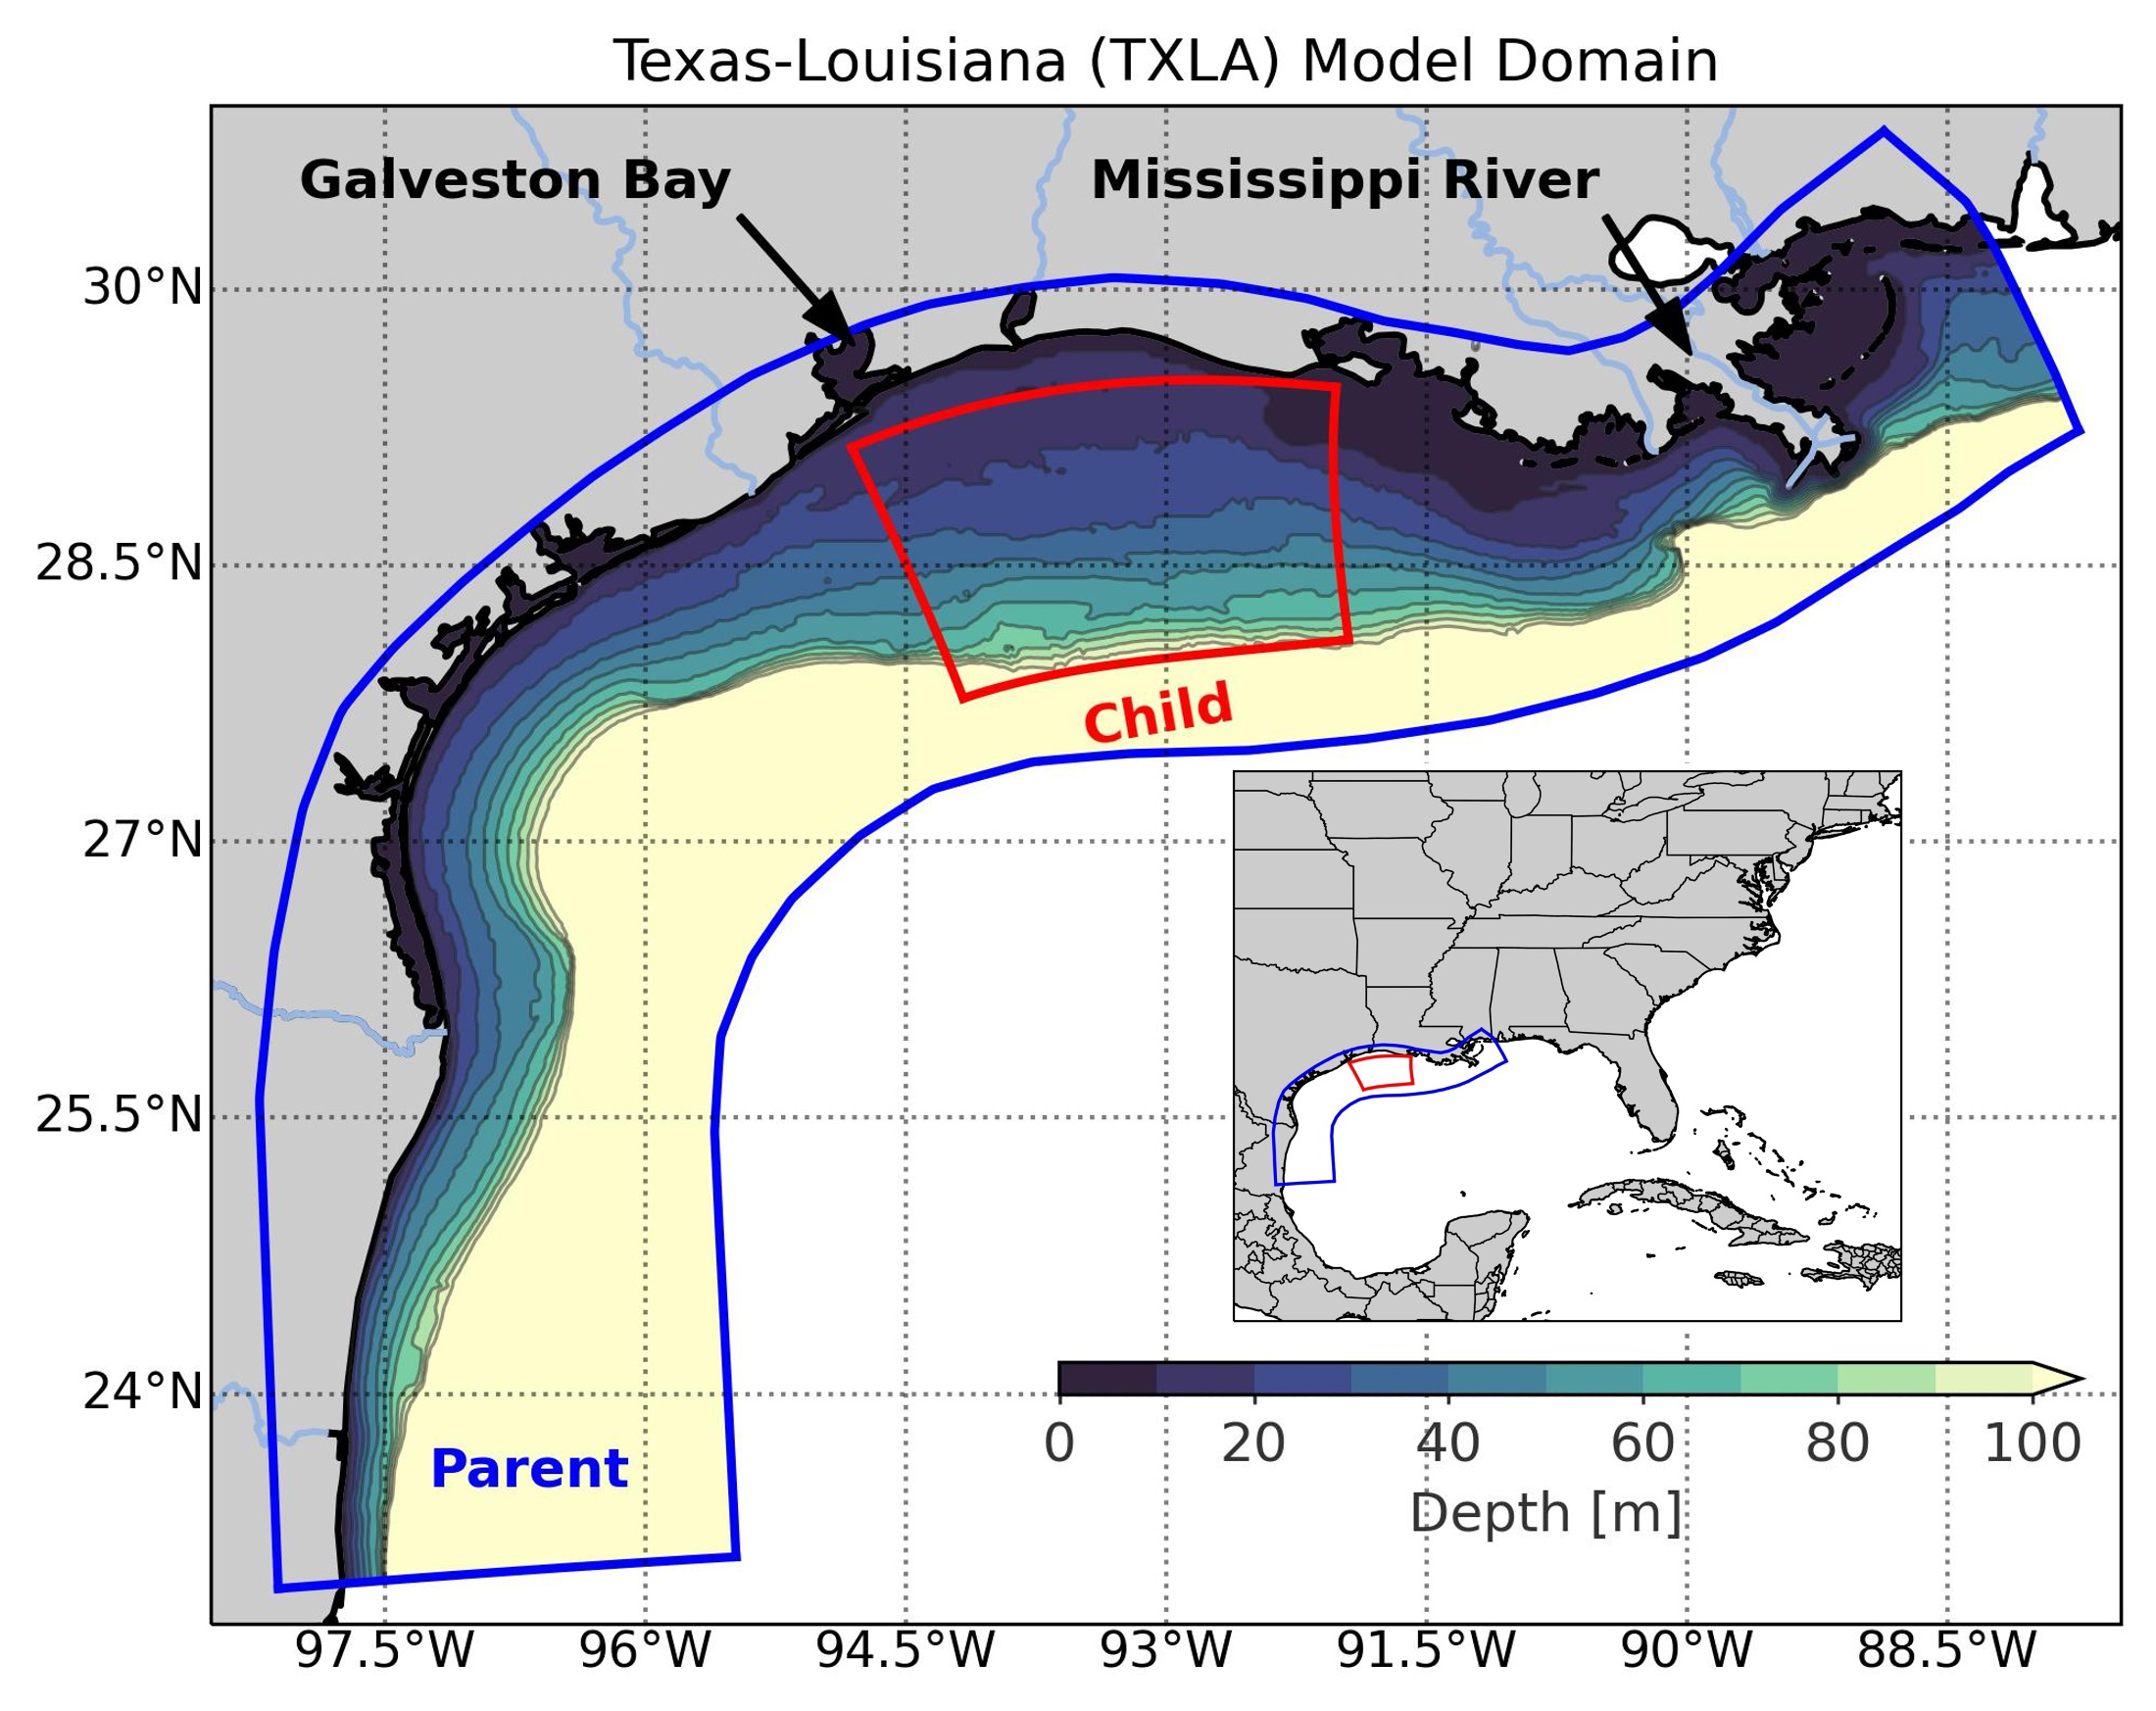
\includegraphics[width=0.9\textwidth]{figures/james_2023/Figure1_domain.jpg}}
    \caption{TXLA parent (coarse) and child (fine) model domain outlined with the blue and red lines, respectively. The colorbar displays the model bathymetry with a basemap located above the colorbar.}
    \label{fig:domain_overview}
\end{figure}

A third-order upwind scheme and a fourth-order centered scheme are used for momentum advection and Multidimensional Positive Definite Advection (MPDATA) is used for tracer advection \citep{Smolarkiewicz_1998}. The $k-\omega$ scheme is used for vertical mixing \citep{umlauf2003extending, Warner_2005} and horizontal mixing is parameterized along geopotential surfaces with constant horizontal viscosity (5.0 m$^2$s$^{-1}$) and diffusivity (1.0 m$^2$s$^{-1}$) values, both of which are scaled to the grid size. The model uses a baroclinic timestep of 75 s and a barotropic timestep of 1.875 s. The model provides hourly output and neglects tides because they are weak over the region \citep{DiMarco_1998}. The model is one-way nested into Global HYCOM Reanalysis to provide open boundary forcing and uses ERA-Interim datasets to provide surface forcing \citep{Dee_2011}. Additionally, the model uses streamflow data from nine rivers to provide freshwater forcing: Sabine, San Antonio, Trinity, Brazos, Calcasieu, Lavaca, Nueces, including the Mississippi and Atchafalaya, which provides the bulk of the discharge. The streamflow salinity is set to zero at all rivers and streamflow temperature is estimated using the bulk approach described by \citep{Stefan_1993}.

The nested model is configured to be two-way such that variables are exchanged across the open boundary. The bathymetry and vertical grid parameters of the child domain are the same as the parent's because the child domain was created from the parent domain. The bathymetry of the child domain was obtained by linearly interpolating the bathymetry of the parent domain. The ratio of the nesting is five to one, resulting in a mean horizontal resolution in the child model of 315 m. The surface fluxes, open boundaries and initial conditions were also obtained from the parent model by interpolating the parent model outputs to the child grid. By doing so, the models can reduce initialization shocks typically seen at the beginning of the simulation. A comparison between the parent and child grids along the open boundaries (i.e., contact points) showed that the fluxes in and out of the boundaries were internally conserved. 

The model has been used in several recent studies focusing on small-scale processes and dynamics in the nGoM \citep{Kobashi_2020,Qu_2021, Qu_2022_NIW, qu2022rapid, Xomchuk_2020}. For this study, we focus our analysis to the location of the child grid (Fig. \ref{fig:domain_overview}). The region is located west of the M/A river discharge points, which contribute to the generation of a baroclinic current over the shelf. The region is often saturated with eddies during summer (Fig. \ref{fig:surface_snapshots} e-f) due to formation of baroclinic instabilities \citep{Hetland_2017,Zhang_2012_numerical}. A diurnal land-sea breeze in near-resonance with the local inertial period forces near-inertial motions (e.g., waves and oscillations) that are perturbed by surface and river forcing \citep{zhang2009near}. The volume-integrated flow is strongly time dependent and serves as an excellent test case to investigate the accuracy of the offline methods in a realistic simulation. Previous studies focusing on submesoscale processes in the nGoM \citep{Barkan_2017,Luo_2016} have primarily focused east of the M/A discharge points in the aftermath of the 2010 \textit{Deepwater Horizon} oil spill. The wave-mean flow interactions in our study region can enhance mixing and lead to the rapid vertical exchange of biogeochemical tracers (e.g., oxygen), which becomes more pronounced as the horizontal resolution increases \citep{qu2022rapid}. We anticipate significant numerical mixing due to strong salinity gradients (Fig. \ref{fig:surface_snapshots} a-d), particularly near the northeastern boundary of the child domain where the Atchafalaya plume is more prevalent. 

\subsection{Simulation overview}

We performed two numerical simulations: one of the native TXLA model without nesting (hereinafter the ``coarse" simulation), and the second with nesting turned on (hereinafter the ``fine" simulation). Both simulations are analyzed from June 3 to July 13, 2010. Due to file corruption issues during the restart process of the fine simulation, we removed the following times (in UTC) from both the coarse and fine grid simulations when directly comparing the simulations: June 17 22:30 to June 18 19:30, June 19 14:30 to 19:30, and July 9 18:30. 

There are several notable mixing events driven by a combination of surface salt fluxes, wind stress, and freshwater input that otherwise contrast with periods of low physical mixing, allowing us to study numerical mixing under a variety of different environmental conditions. Over the inner shelf during the study period, contributions to density variations from variation in the temperature field are small relative to those from salinity variations. We focus our analysis to metrics that influence numerical mixing, in particular different metrics from the velocity gradient tensor normalized by the Coriolis parameter such as vertical relative vorticity $\zeta/f$, horizontal divergence $\delta/f$, horizontal strain rate $\alpha/f$, and the horizontal salinity gradient magnitude $|\nabla_H s|$. They are defined as:
\begin{equation}
    \zeta/f = \bigg(\frac{\partial v}{\partial x} - \frac{\partial u}{\partial y}\bigg)/f \quad ,
\end{equation}
\begin{equation}
    \delta/f = \bigg(\frac{\partial u}{\partial x} + \frac{\partial v}{\partial y}\bigg)/f \quad ,
\end{equation}
\begin{equation}
    \alpha/f = \sqrt{\bigg(\frac{\partial u}{\partial x} - \frac{\partial v}{\partial y}\bigg)^2+\bigg(\frac{\partial v}{\partial x} + \frac{\partial u}{\partial y}\bigg)^2}/f \quad ,
\end{equation}
\begin{equation}
    |\nabla_H s| = \sqrt{\bigg(\frac{\partial s}{\partial x} \bigg) ^2 + \bigg(\frac{\partial s}{\partial y} \bigg)^2} \quad .
\end{equation}
To isolate the effects of nesting on model processes, all variables discussed hereinafter from the coarse grid are subsetted offline to the location of the child grid and compared directly with the child grid of the fine simulation. Fig. \ref{fig:surface_snapshots} displays a sample of surface fields for the coarse and fine simulations of salinity, $|\nabla_H s|$, $\zeta/f$, $\delta/f$, and $\alpha/f$ during a time where numerous eddies are seen over the shelf. These eddies are considered to be submesoscale because they exhibit $\mathcal{O}(1)$ surface Rossby numbers, as approximated by $\zeta/f$ \citet{Barkan_2017, Kobashi_2020, McWilliams_2016}. The salinity of the fine simulation exhibits subtle differences near the northeastern boundary, however the effects of nesting are more striking in the vorticity. Several frontal eddies with anticyclonic cores and cyclonic filaments are resolved by both simulations. The cyclonic filaments are often associated with frontal convergence \citep{Kobashi_2020, qu2022rapid} and salinity gradients orders of magnitude stronger than those found in the anticyclonic cores where the the salinity is more homogeneous. The horizontal strain rate is enhanced throughout the fine simulation, which acts to sharpen the horizontal salinity gradients and enhance frontogenesis \citep{Hoskins_1972}.

\begin{figure} 
 \centerline{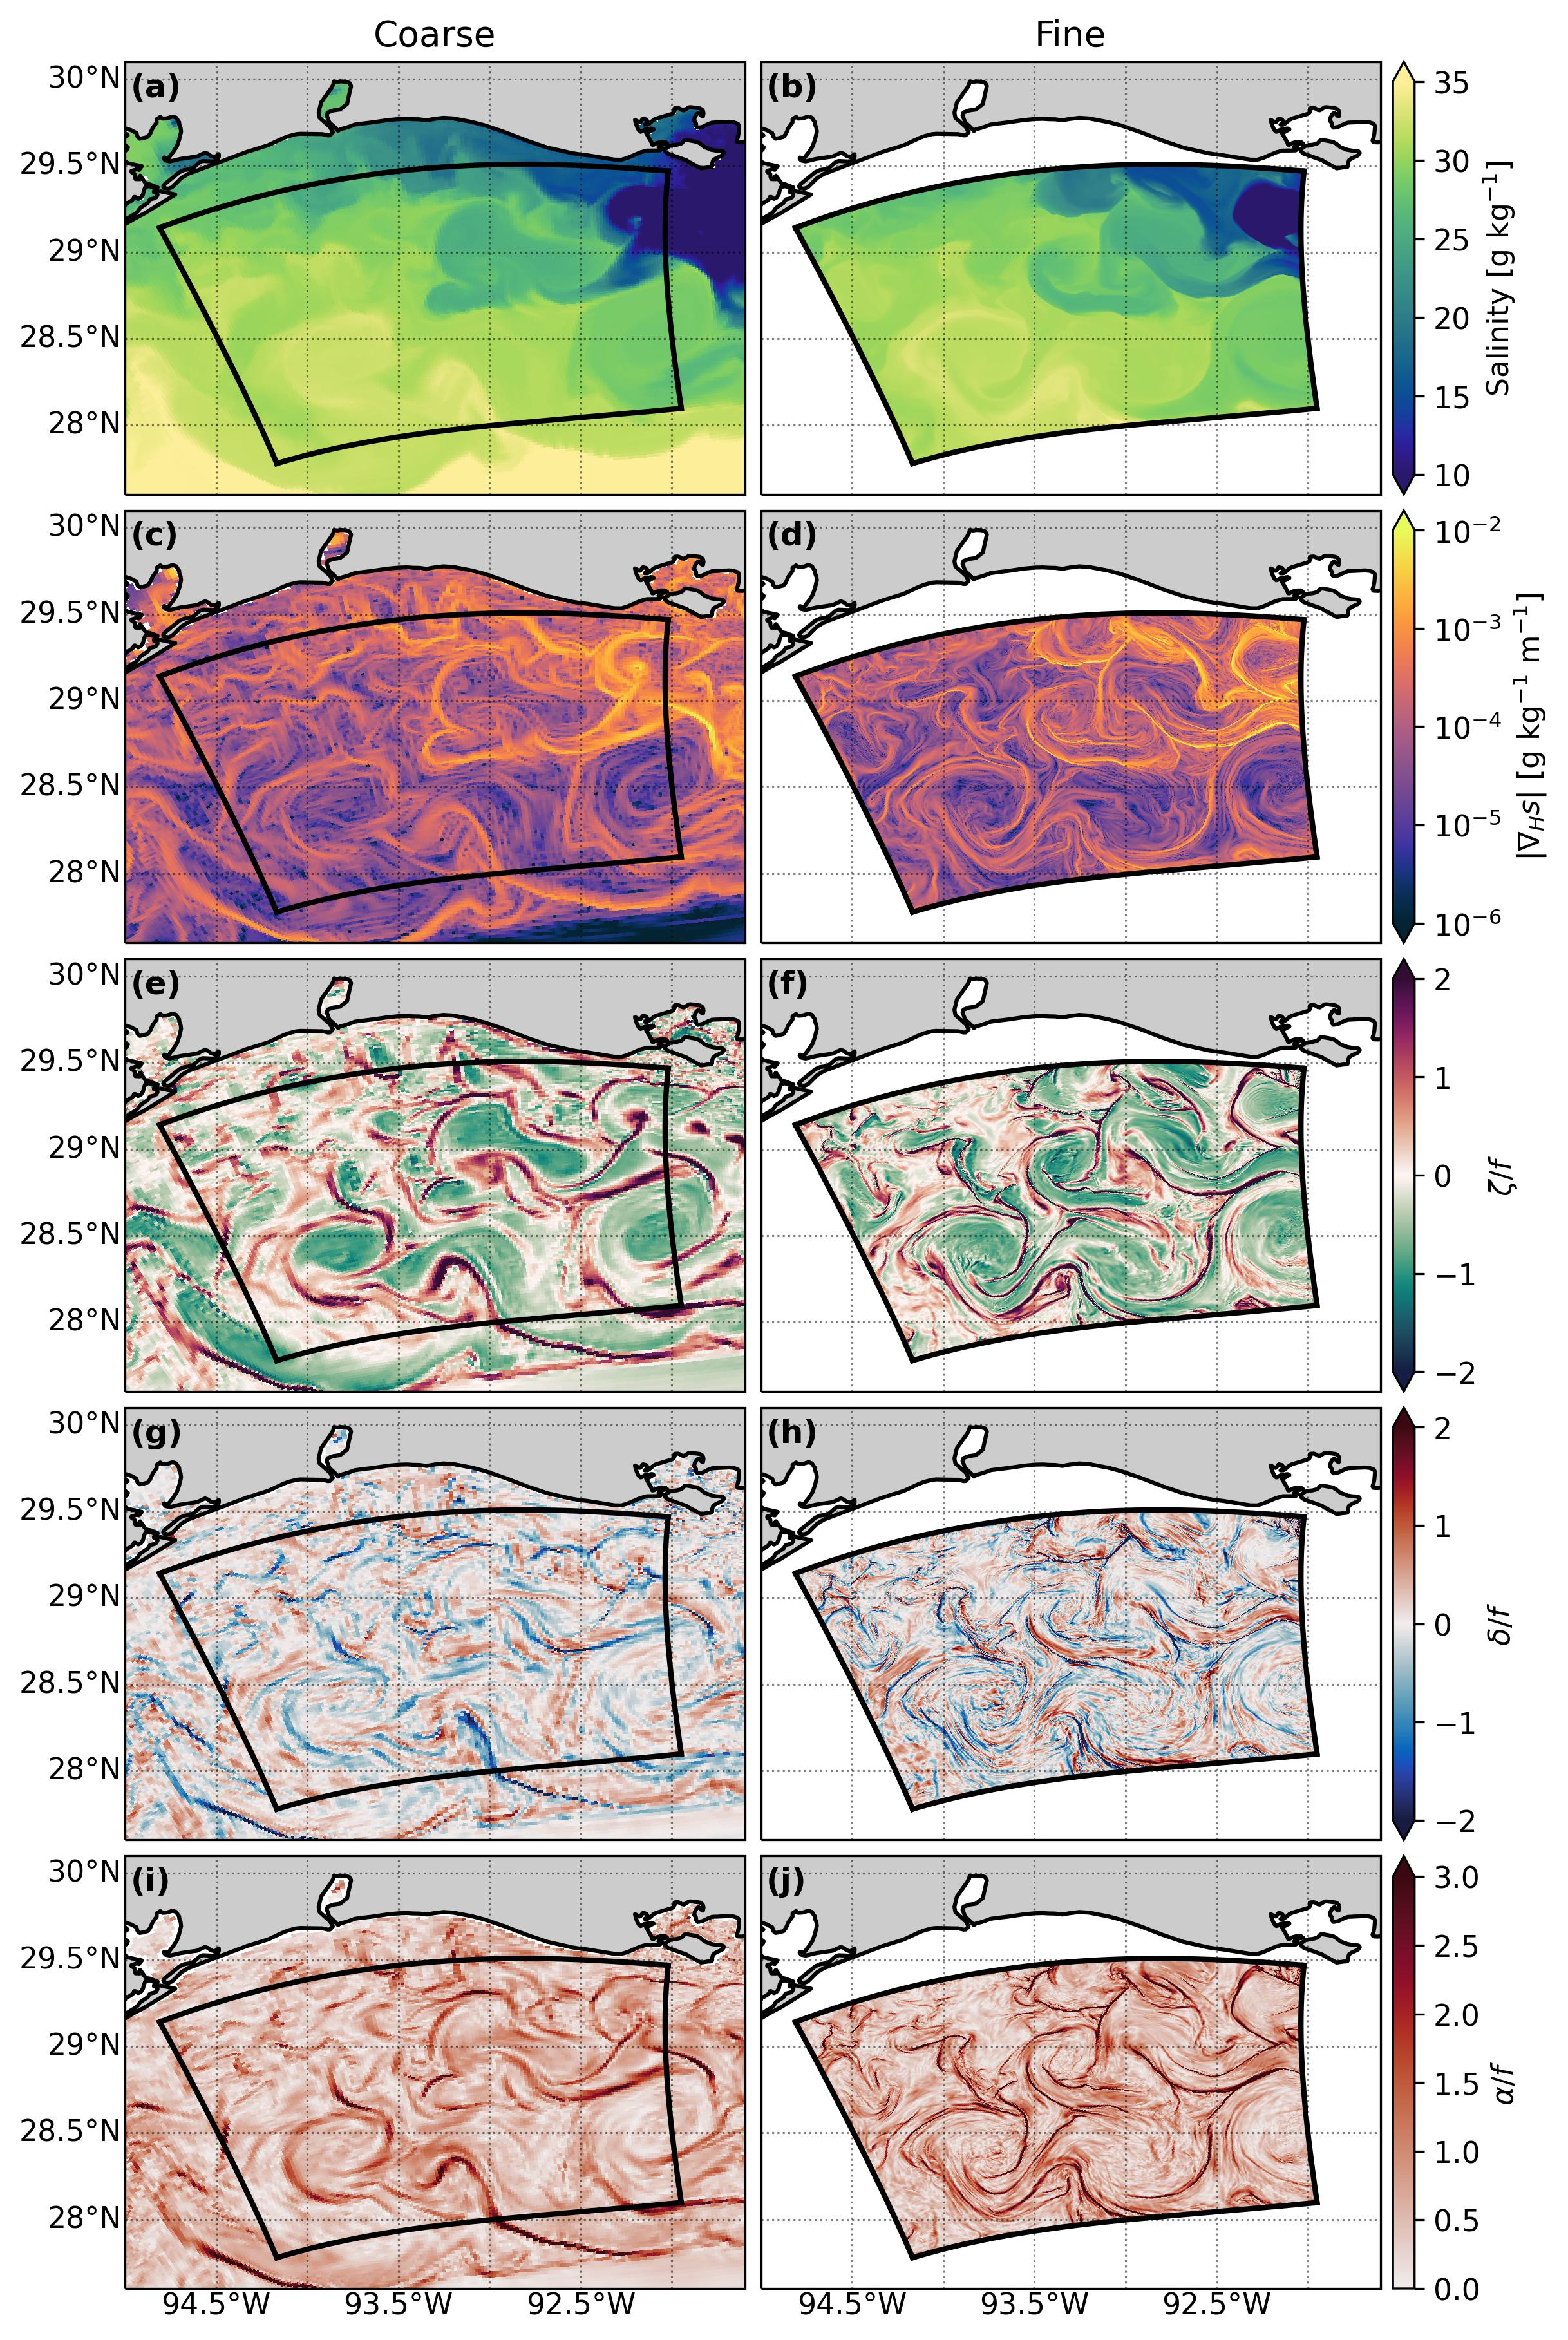
\includegraphics[width = 0.85\linewidth]{figures/james_2023/Figure2_snapshot.jpg}}
  \caption{Surface fields on June 20, 2010 12:30 UTC for the coarse (left column) and fine (right column) simulations of salinity (a-b), horizontal salinity gradient magnitude $|\nabla_H s|$ (c-d), relative vertical vorticity $\zeta/f$ (e-f), horizontal divergence $\delta/f$ (g-h), and horizontal strain rate $\alpha/f$ (i-j). Note that all velocity gradient tensor quantities are normalized by the Coriolis parameter $f$ and all variables are defined in text.}
  \label{fig:surface_snapshots}
\end{figure} 

To better understand the impacts of nesting on surface processes, Fig. \ref{fig:surface_pdfs} displays probability density functions (PDFs) of the various properties discussed above. Fig. \ref{fig:surface_pdfs} also displays the latter three quantities sorted by $\zeta/f>1$, which correspond to $\mathcal{O}(1)$ surface Rossby numbers associated with submesoscale fronts. The associated median and median-skewness of the velocity gradient tensor quantities and $|\nabla_H s|$ are shown in Table \ref{tab:1}. The relative vorticity is skewed cyclonically (positively) with a negative median for both simulations, with the median of the fine simulation decreasing by 159$\%$ and skewness increasing by 31\%. The divergence for both simulations have positive medians (i.e., divergence) and negative skewnesses, with the fine simulation increasing over 260\% and the skewness decreasing by 34\%. The strain for both models follows a $\chi$ distribution, consistent with the results of \citet{Shcherbina_2013}. The salinity gradient magnitude of the fine simulation has a slightly smaller median and skewness compared to the coarse simulation. When sorted by $\zeta/f>1$, the latter three quantities have significantly higher probabilities towards the tails of their distributions. This makes intuitive sense because the submesoscale fronts are associated with strong horizontal salinity gradients, elevated convergence/divergence, and elevated strain \citep{McWilliams_2016}. Interestingly, PDFs of $|\nabla_H s|$ remain essentially unchanged between the coarse and fine simulations, with slightly stronger gradients at the tail of the fine distribution, suggesting that changes to the velocity gradients do not necessarily result in similar changes to the salinity gradients. 

A possible explanation for the relatively unchanged salinity gradients in the nested model is due to the horizontal mixing scheme. ROMS scales grid-dependent horizontal diffusivities as
\begin{equation} \label{eq:kappa_H}
    \kappa_H = \frac{\kappa_{0}}{\max \sqrt{dA}}\sqrt{dA},
\end{equation}
where $\kappa_0$ is a prescribed background turbulent diffusivity (specified previously) and $dA$ is the lateral grid cell area. The maximum grid cell area is unique to each model grid, resulting in $\kappa_H$ being twice as large on average in the fine simulation compared to the coarse. As we will show in Section \ref{sec:results}, this increases the magnitude of the horizontal mixing and turbulent diffusion significantly, which may prevent the horizontal salinity gradients from sharpening as expected. 

\begin{figure}[ht] 
 \centerline{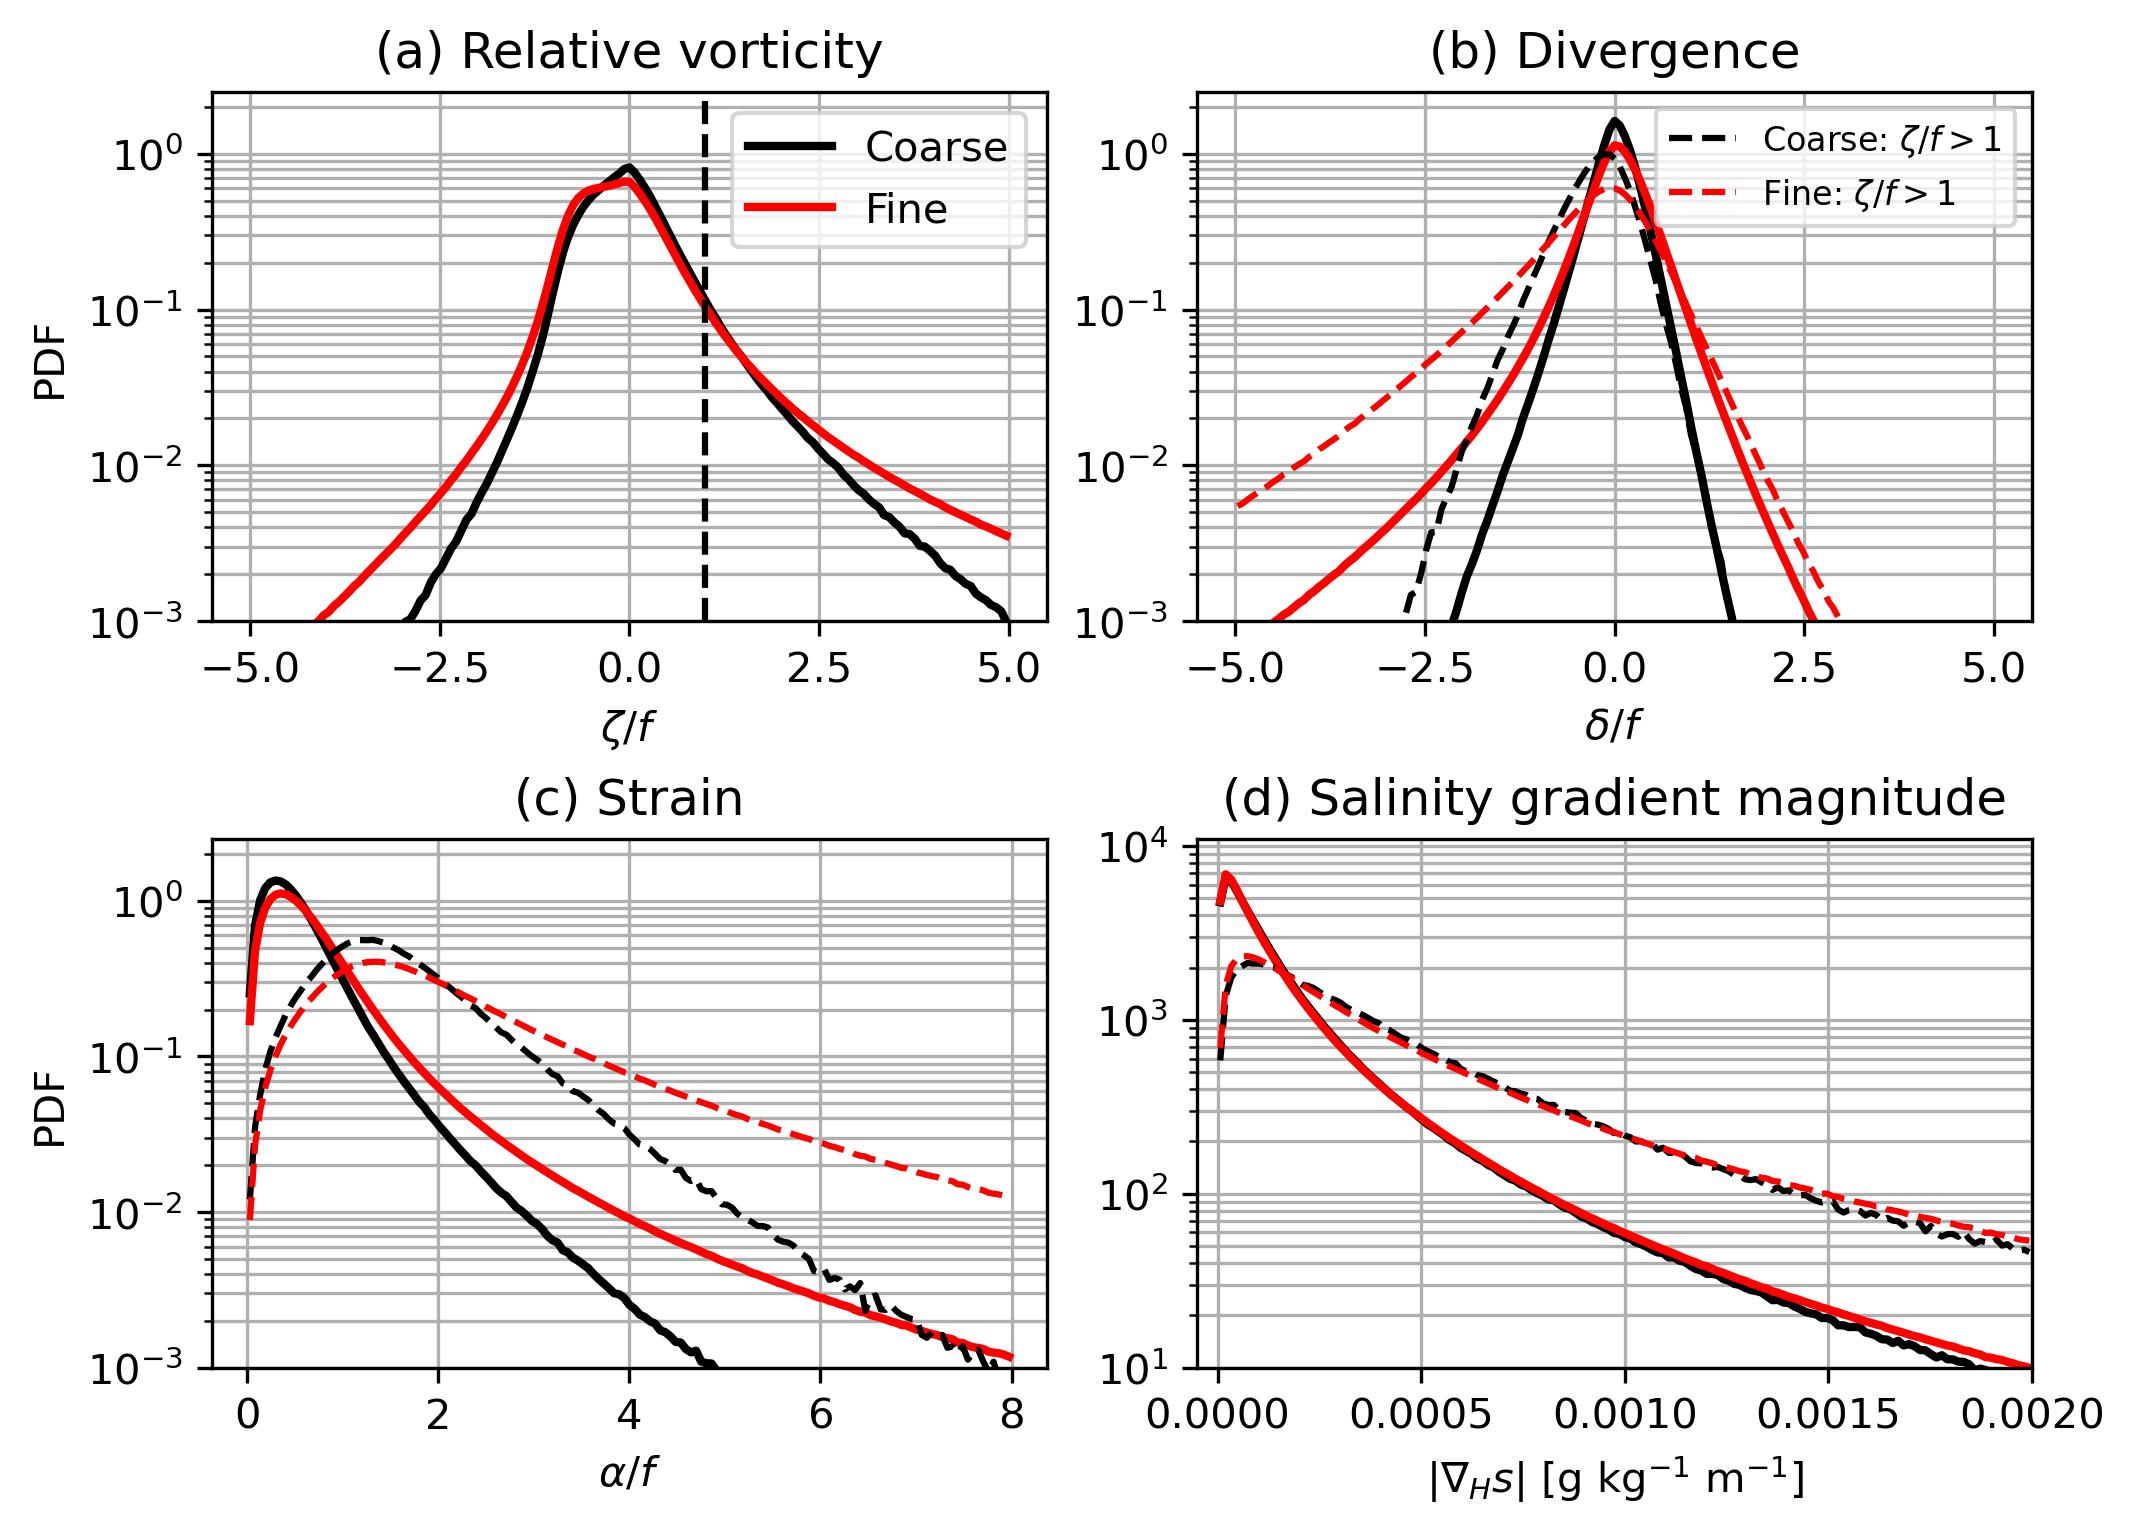
\includegraphics[width = \linewidth]{figures/james_2023/Figure3_surface_pdfs.jpg}}
  \caption{Probability density functions (PDFs) of surface $\zeta/f$ (a), $\delta/f$ (b), $\alpha/f$ (c), and $|\nabla_H s|$ (d) for the entire simulation period as defined in text. Dashed lines display $\delta/f$, $\alpha/f$, and $|\nabla_H s|$ sorted by $\zeta/f>1$ corresponding to the model fronts. The black dashed line in (a) demonstrates where $\zeta/f=1$. Each PDF was constructed discretely using 150 equal-spaced bins by first computing histograms and then normalized so the PDFs integrate to one.}
  \label{fig:surface_pdfs}
\end{figure}

 \begin{table}[h]
    \caption{Median and Pearson's median skewness for the surface and whole water column $\zeta/f$, $\delta/f$, $\alpha/f$, and $|\nabla_H s|$ for the coarse and fine simulations. Median quantities are denoted by an overline, and skewness quantities are denoted by a tilde. Median and skewness of the whole water column were computed by subsampling the coarse simulation every three $\xi, \eta \, (x,y)$ points and the fine simulation every 15 $\xi, \eta$ points. Note $|\nabla_H s|$ medians have units of g kg$^{-1}$ m$^{-1}$.}
    \centering
        \begin{tabular}{c c c c c c c c c}
        \hline
         Simulation & $\overline{\zeta/f}$ & $\widetilde{\zeta/f}$  & $\overline{\delta/f}$ &
         $\widetilde{\delta/f}$ &
         $\overline{\alpha/f}$  &
         $\widetilde{\alpha/f}$ & 
         $(\overline{|\nabla_H s|})*10^4$  &
         $\widetilde{|\nabla_H s|}$ \\
        \hline
         Coarse: Surf. & -0.054 & 0.296 & 0.009 & -0.154 & 0.470 & 0.757 & 1.000 & 0.926 \\
         Fine: Surf. & -0.140 & 0.399 & 0.0346 & -0.206 & 0.576 & 0.756 & 0.989 & 0.805 \\
         Coarse: Whole & -0.002 & 0.092 & 0.002 & -0.049 & 0.405 & 0.767 & 0.905 & 0.884 \\
         Fine: Whole &  -0.026 & 0.144 & 0.008 & -0.064 & 0.497 & 0.801 & 1.02 & 0.839 \\
        \hline
         \end{tabular} 
         \label{tab:1}
 \end{table}
 
Trends remain similar for the entire water column (Fig. \ref{fig:whole_pdfs}), however the distributions of $\zeta/f$ and $\delta/f$ are slightly more Gaussian. $\alpha/f$ still follows a $\chi$ distribution, but is significantly weaker relative to the surface distribution.  $|\nabla_H s|$ changes modestly compared to the velocity gradients, with the coarse simulation having slightly larger salinity gradients near the tails of the distribution. 

\begin{figure}[ht] 
 \centerline{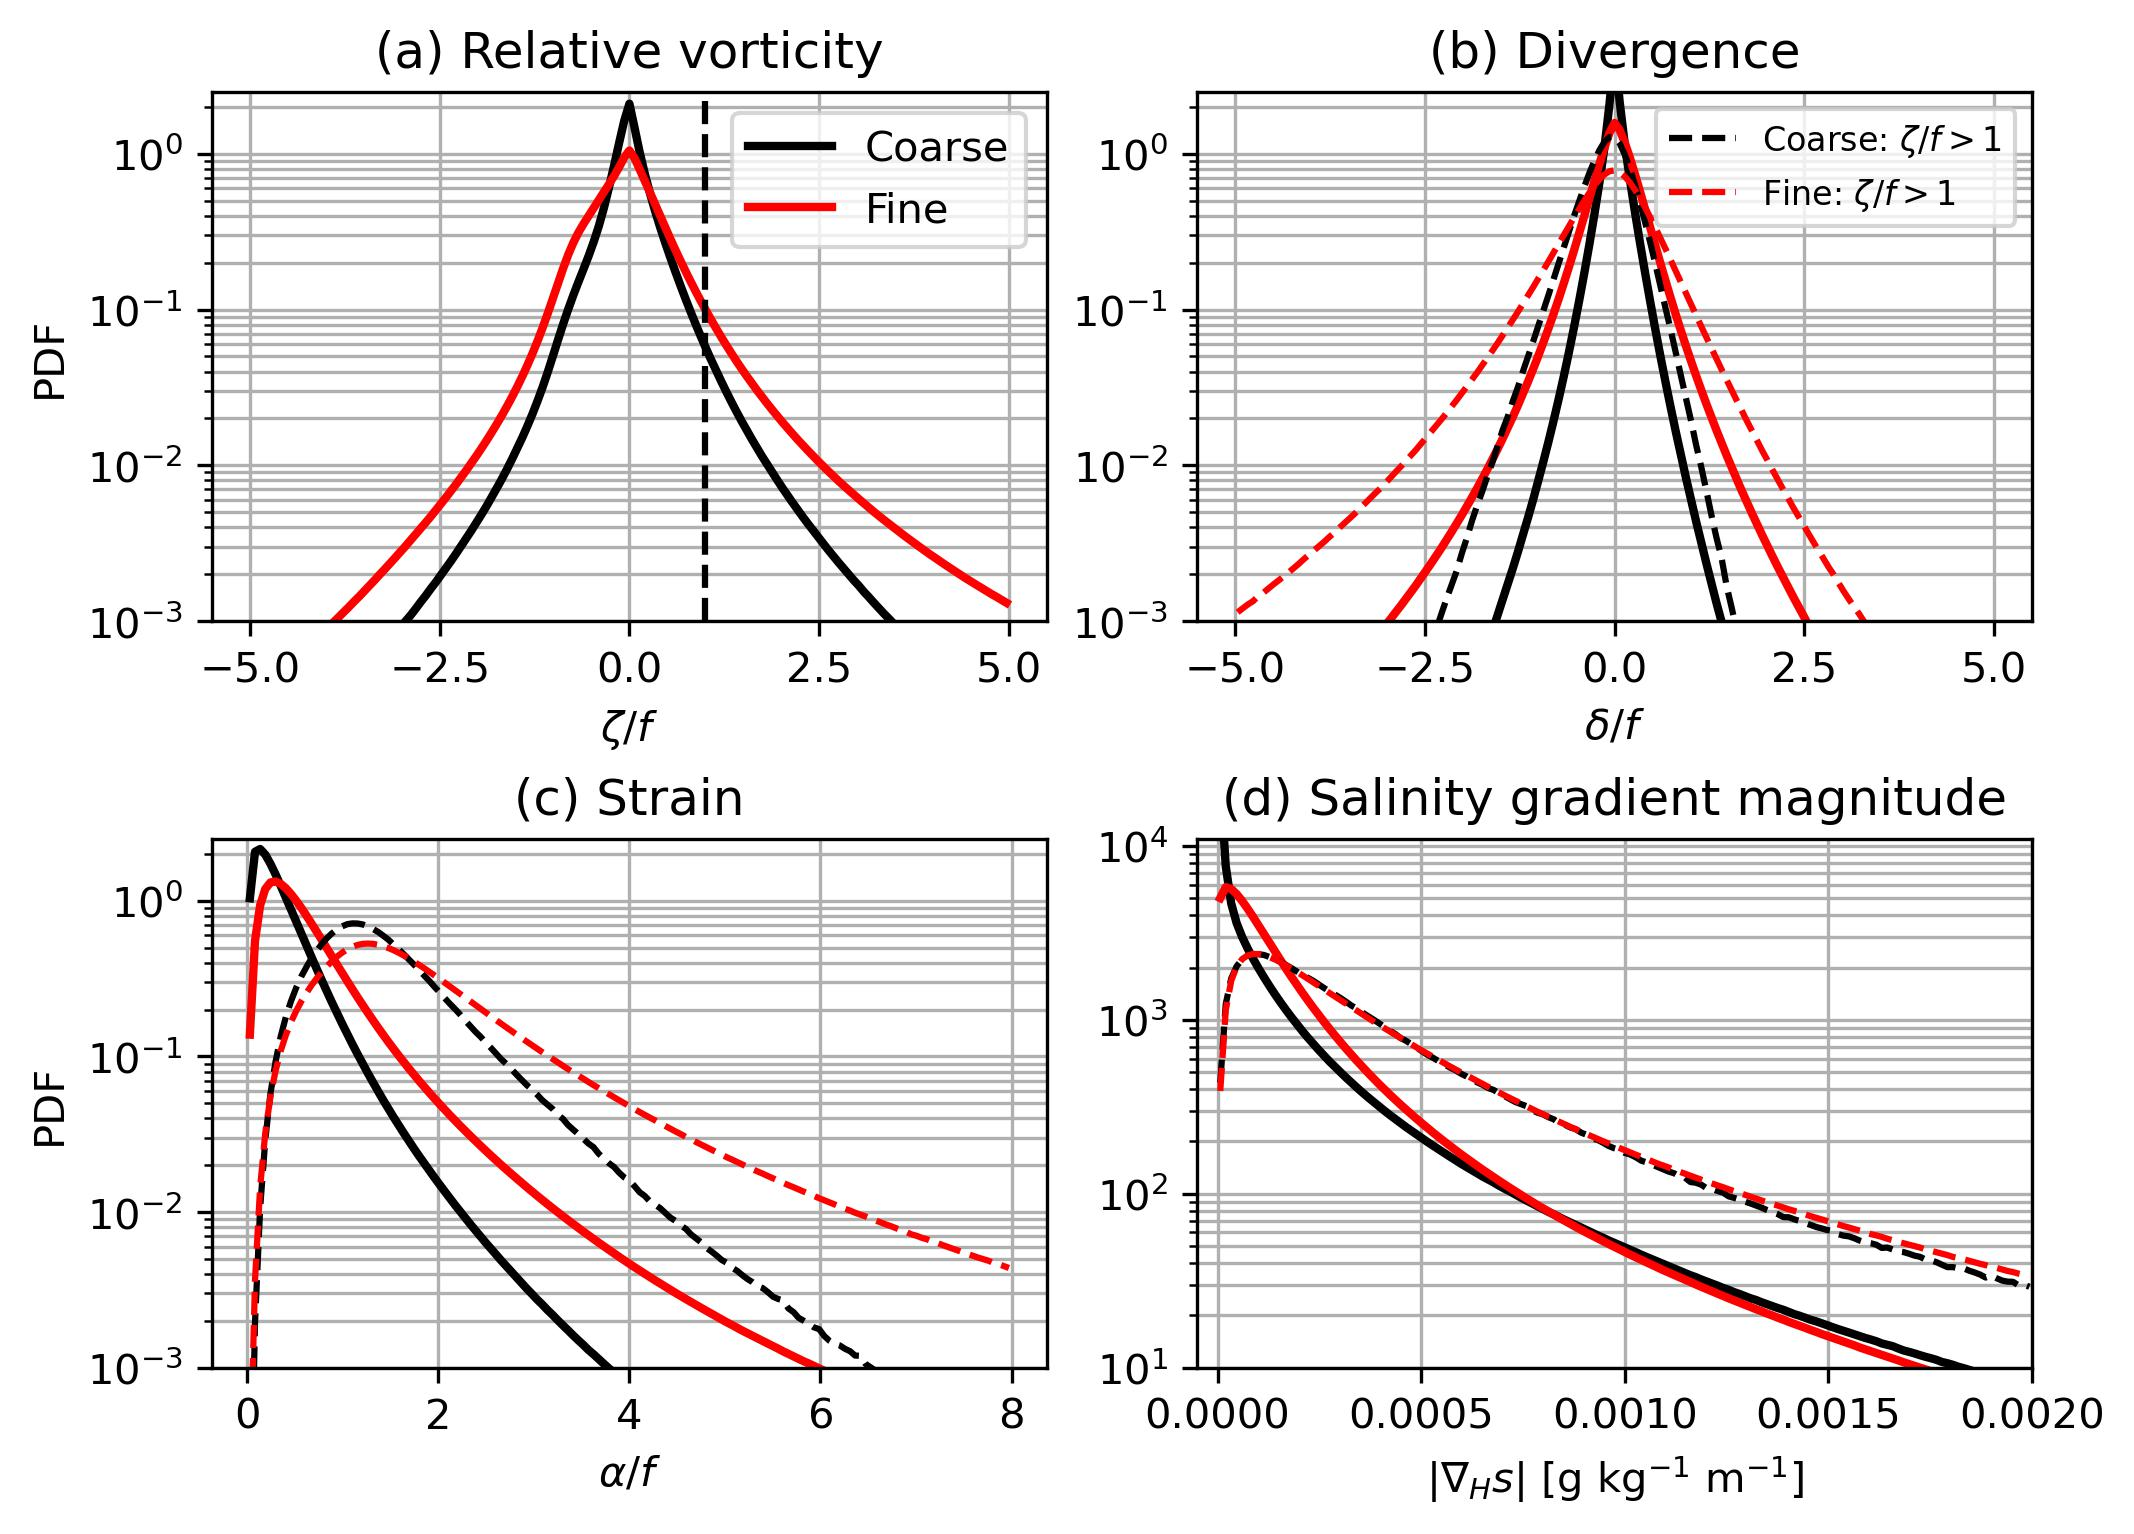
\includegraphics[width = \linewidth]{figures/james_2023/Figure4_whole_pdfs.jpg}}
  \caption{Same as Fig. \ref{fig:surface_pdfs}, but for the entire water column.}
  \label{fig:whole_pdfs}
\end{figure}

\subsection{Implementation of the online method for numerical mixing}

The online numerical mixing $\mathcal{M}_{num, on}$ is calculated locally following \citet{Burchard_2008}:   
\begin{equation}\label{Eq:mnum_online}
    \mathcal{M}_{num, on} = \frac{A\{ s^2 \}-\left(A \{s \} \right)^2}{\Delta t} \quad ,
\end{equation}
where $A$ is the advection operator (i.e., MPDATA) and $\Delta t$ is the model time step, which yields the numerical mixing in each grid cell. A discretized version of Eq. \ref{Eq:mnum_online} may be found in \citet{Burchard_2008}. $\mathcal{M}_{num, on}$ is computed using $s$ as the representative tracer instead of $s^{\prime}$ because $s^{\prime}$ requires calculating $\overline{s}$ for the location of the child grid during the model run. An analysis (not shown) of Eq. \ref{Eq:mnum_online} for a first order upwind scheme suggests that $\mathcal{M}_{num,on}$ should be identical whether $s$ or $s^\prime$ is used as the tracer. However, this is not necessarily the case for higher-order, nonlinear advection schemes that employ more sophisticated numerical algorithms. Therefore, it is unclear whether the online method should converge to $\mathcal{M}_{num, s^{\prime^2}}$ in addition to $\mathcal{M}_{num, s^2}$ if offline discretization errors are small. 

Although we will use the relative agreement between on- and offline methods as the basis to assess this, other sources of spurious mixing such as spurious convection due to high grid cell Reynolds numbers \citep{ilicak2016quantifying, Ilicak_2012}, cabbeling, and numerical diffusion may potentially contaminate both on- and offline methods. Generally, we do not expect these sources to be significant based on the results of \citet{Wang_2021}. We do not expect spurious convection to be significant because ROMS employs a third-order upstream advection scheme that enforces small grid-scale Reynolds numbers \citep{Ilicak_2012,shchepetkin2005regional}. Cabbeling is also not likely to be an issue, as work by \citet{barkan2017submesoscalepart2} slightly east of our study area suggested it is less significant in the M/A plume compared to other oceanic regions. However, we cannot say \textit{a priori} whether numerical diffusion will be significant. We will revisit these comments in Sections \ref{sec:results}-\ref{sec:discussion}. The numerical implementation of the offline method is shown in \ref{Appendix:offline_method}.

\section{Results} \label{sec:results}

\subsection{Spatial structure of the numerical and physical mixing}

To motivate our analysis of the physical and numerical mixing, Fig. \ref{fig:cross_section} displays cross-sections of $\mathcal{M}_{num, on}$ and $\chi^s$ split into horizontal and vertical components when a strong cross-shelf density gradient is generated by freshwater input for the coarse and fine simulations. A nearshore and offshore pycnocline are observed, where the nearshore pycnocline near 29$^\circ$N is associated with freshwater input from the Atchafalaya River and the offshore near pycnocline is associated with freshwater input from the Mississippi River \citep{Kobashi_2020}. The numerical mixing, although noisy, is approximately 2.75 times larger when averaged over the cross section in the coarse simulation compared to the physical mixing and may be orders of magnitude larger locally. The negative mixing is due to the anti-diffusive properties of MPDATA, which acts to reduce the total mixing but does not have a physical interpretation. The numerical mixing is concentrated primarily where the isopycnals are pinched in the pycnoclines, generally corresponding to strong horizontal salinity gradients. Stronger salinity gradients are located shoreward of 29.25$^{\circ}$N, however the numerical mixing is small relative to the offshore pycnocline, likely due to increased grid resolution. Previous studies have shown that numerical mixing is related to the horizontal salinity gradients \citep{hofmeister2011realistic, Kalra_2019, Klingbeil_2014,Wang_2021} and we investigate this more in Section \ref{sec:discussion}.

\begin{figure}
 \centerline{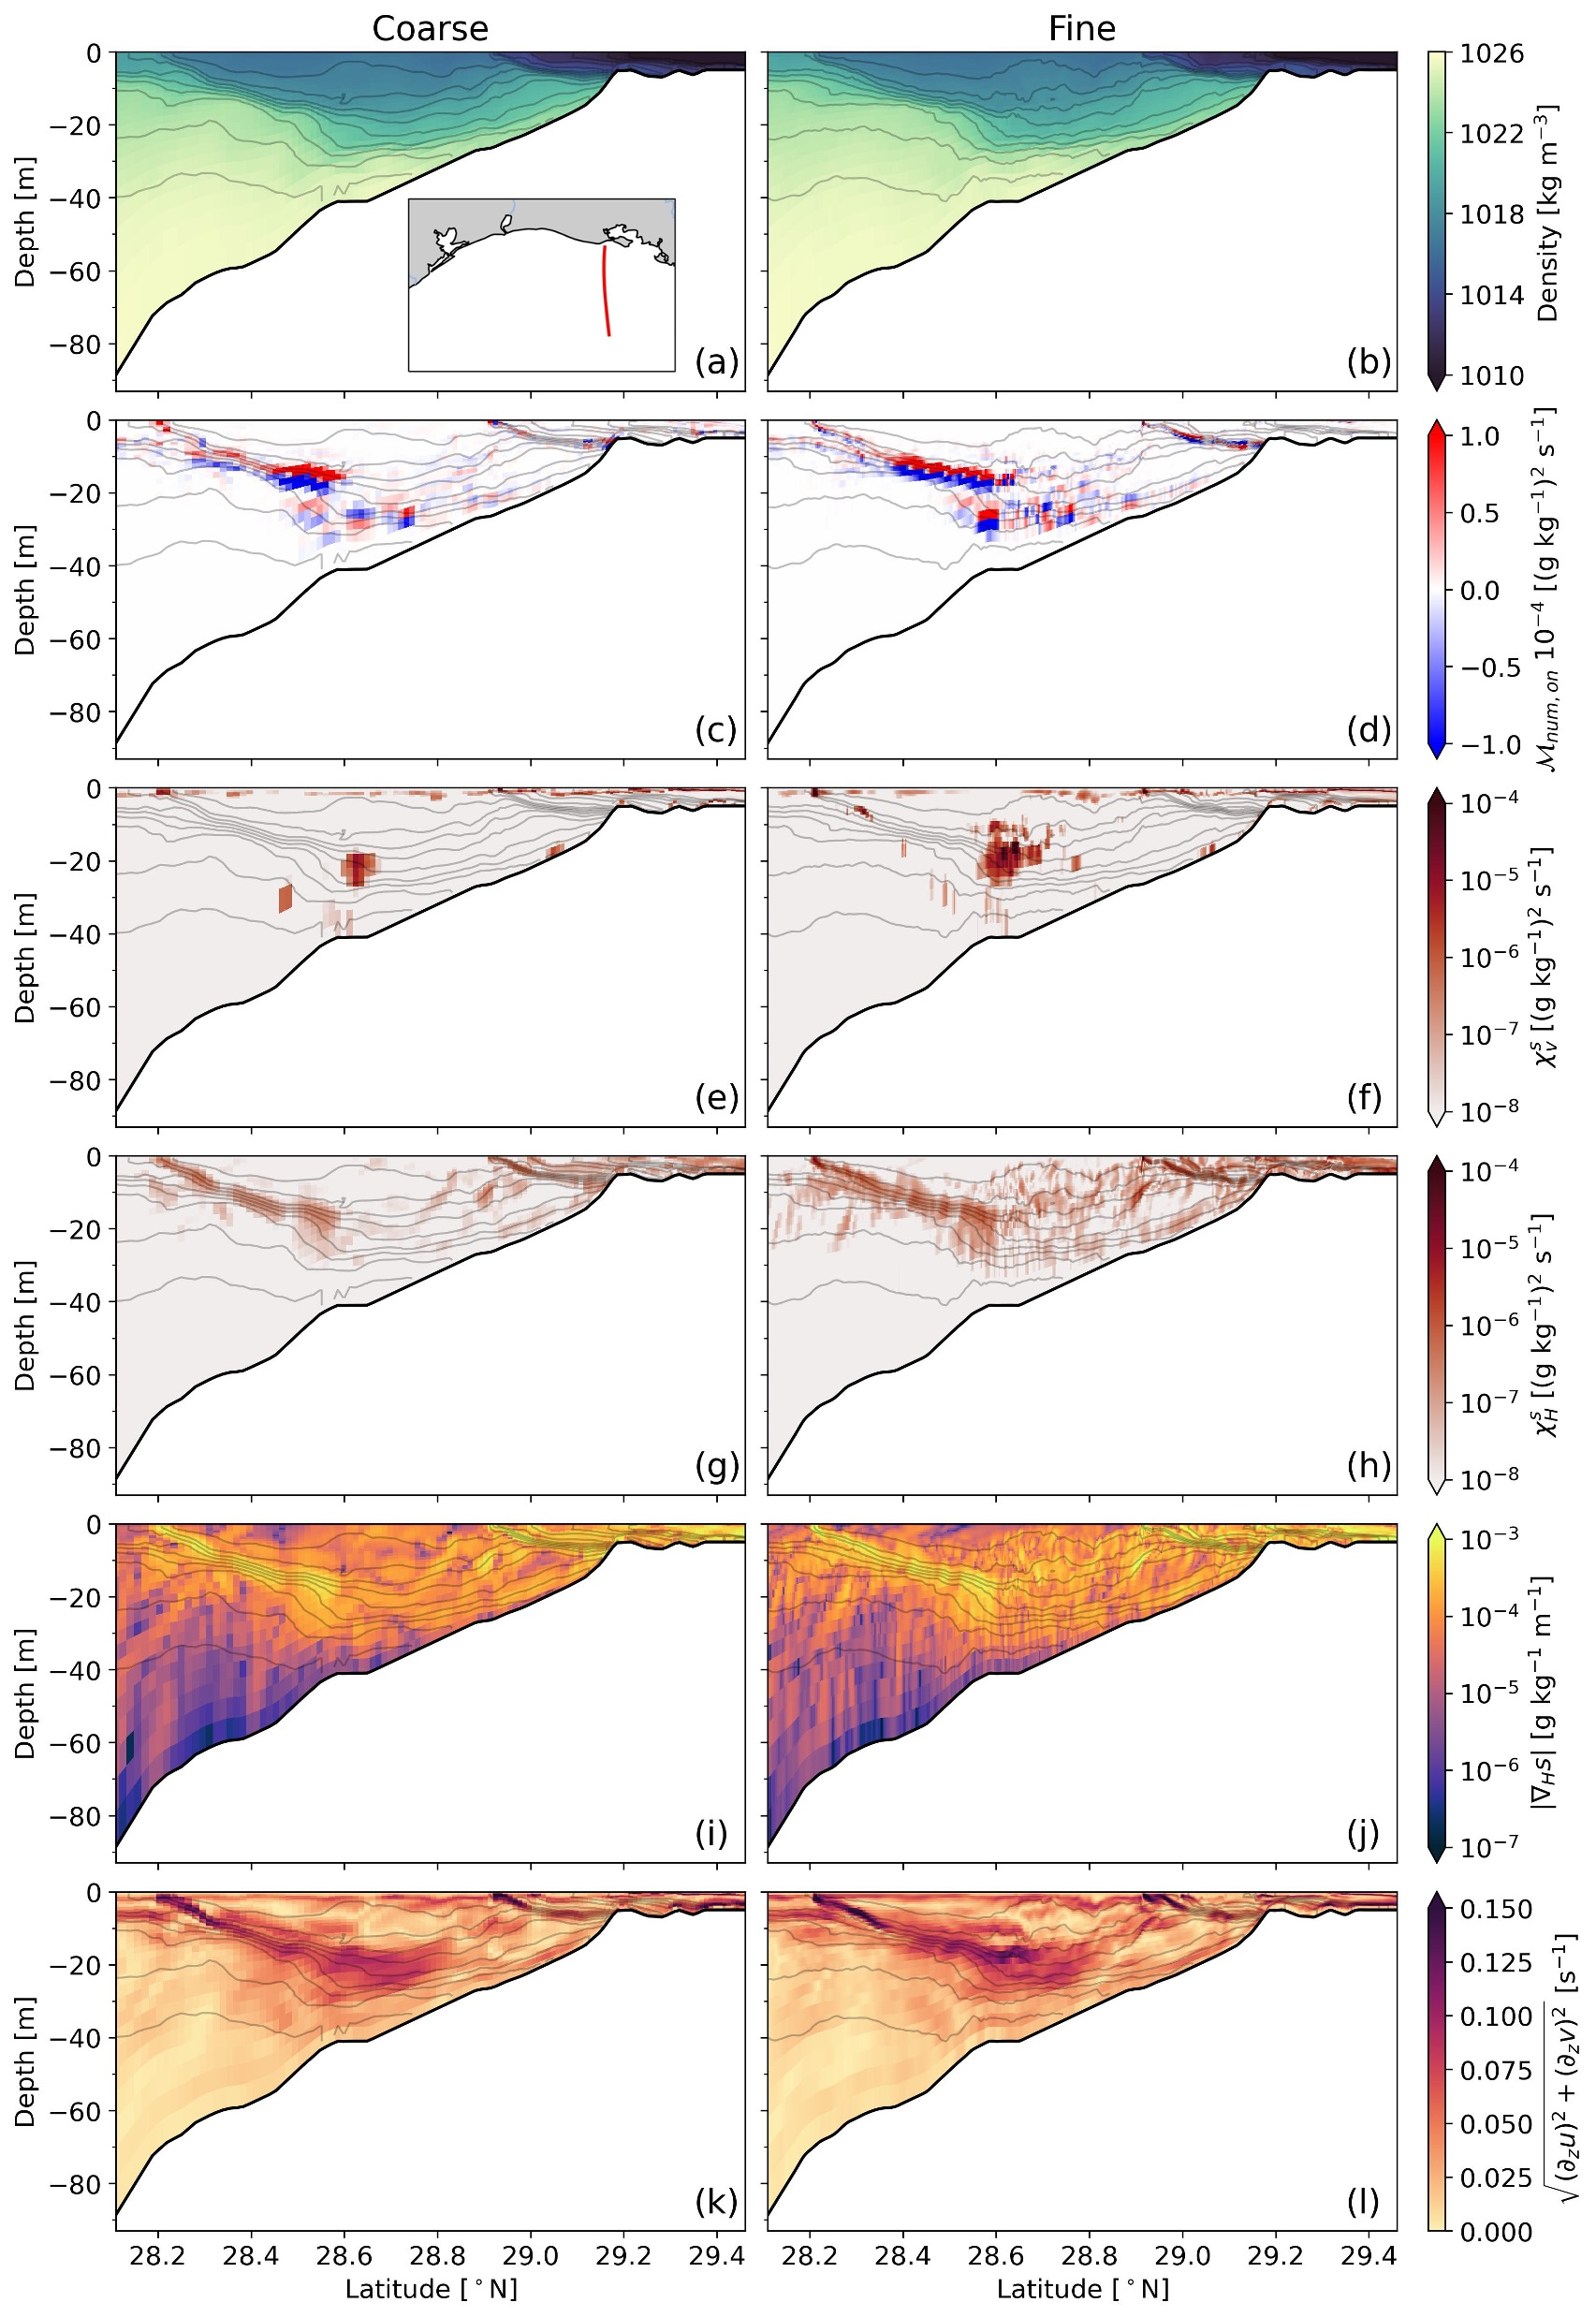
\includegraphics[width = 0.85\linewidth]{figures/james_2023/Figure5_cross_section.jpg}}
  \caption{Cross-sections for the coarse (left) and fine (right) simulations examining mixing and related properties where a strong cross-shelf density gradient is present on June 8, 2010 00:30 UTC. Density (a-b), $\mathcal{M}_{num, on}$ (c-d), $\chi_v^s$ (e-f), $\chi_H^s$ (g-h), $|\nabla_H s|$ (i-j), and magnitude of vertical shear $\sqrt{(\partial_z u)^2+(\partial_z v)^2}$ (k-l). Isopycnals are displayed with gray lines every kg m$^{-3}$ for the range shown in the colorbar. Note that the numerical mixing is on a linear scale and the physical mixing is on a log scale.}
  \label{fig:cross_section}
\end{figure}

The physical mixing exhibits different spatial trends when broken into horizontal ($\chi_H^s$) and vertical $\chi_v^s$ components. This is due to two reasons: different parameterizations for the horizontal and vertical turbulent diffusivities and different distributions of the horizontal and vertical salinity gradients. $\chi_v^s$ is concentrated at the surface and in the middle of cross-section. The areas of high physical mixing roughly correspond to where the vertical shear and turbulent diffusivity are strong (and large vertical velocity variance). Similar to the numerical mixing, $\chi_H^s$ is strongly correlated with $|\nabla_H s|$ and comprises 9.1$\%$ of the total physical mixing ($\chi_H^s+\chi_v^s$) when averaged over the cross section. 

Model nesting produces several notable differences, although the general trends remain the same. There are several locations where the numerical mixing in the fine simulation is stronger than the coarse simulation. The physical mixing averaged over the cross-section in the fine simulation is larger than the coarse simulation, with $\chi_H^s$ now comprising 24$\%$ of the total physical mixing. As discussed in Section 3, this is primarily due to an increase in the magnitude of $\kappa_H$ in the fine simulation. The spatially-averaged numerical mixing decreases by $51$\%, with the mean numerical mixing being positive for both simulations. In this particular cross-section, the decrease in average numerical mixing appears to be due to a more symmetric distribution of positive and negative values, which is evident in probability density functions and estimates of skewness over the cross-section. Eq. \ref{Eq:mnum_online} is limited in this application because it does not separate the horizontal and vertical contributions of tracer advection to numerical mixing. Horizontal and vertical tracer advection are often computed with different subroutines in ocean models, which could allow $\mathcal{M}_{num, on}$ to be decomposed into components. Such a decomposition could be used to assess whether refinement of the horizontal or vertical grid resolution is required to reduce numerical mixing.

To examine the broader spatial variability, Fig. \ref{fig:depth_integrated} displays depth- and time-integrated $\chi^s$ and $\mathcal{M}_{num, on}$, the ratio of integrated $\chi_H^s$ to $\chi_v^s$, and the ratio of integrated $\mathcal{M}_{num, on}$ to $\chi^s$. Both $\chi_v^s$ and $\mathcal{M}_{num, on}$ are strongest near the northeastern boundary due to a large influx of brackish water from the M/A river plume. $\chi_H^s$ is more significant near the southwestern boundary. This is unsurprising because the vertical salinity gradients will be weaker relative to the horizontal further offshore where the plume stratification is weaker (in contrast to the northeastern boundary). The integrated $\mathcal{M}_{num, on}$ in the coarse simulation is significantly noisier, with a small patch of negative values concentrated near the northeastern boundary. As a consequence, this will decrease the total mixing and may spuriously alter the timescales of mixing processes associated with submesoscale fronts, although more analysis is needed to confirm this. The integrated $\mathcal{M}_{num, on}$ exceeds $\chi^s$ for a significant portion of the domain in the coarse simulation, with the greatest discrepancy occurring near the southwestern boundary where $\chi^s$ is weaker. 

There is a marked enhancement of integrated $\chi^s$ in the fine simulation. This is especially true for the ratio of $\chi_H^s$ to $\chi_v^s$. As discussed previously, we believe this is due to an increase in $\kappa_H$ of the fine simulation. A newly resolved patch of $\chi^s$ in the fine simulation spanning almost half the latitudinal extent of the domain is seen east of $93^{\circ}$W. $\mathcal{M}_{num, on}$ is reduced throughout the domain of the fine simulation. Additionally, the ratio of $\mathcal{M}_{num, on}$ to $\chi^s$ substantially decreases in the fine simulation, with the numerical mixing exceeding the physical mixing in several patches near the southwestern boundary.

\begin{figure}
 \centerline{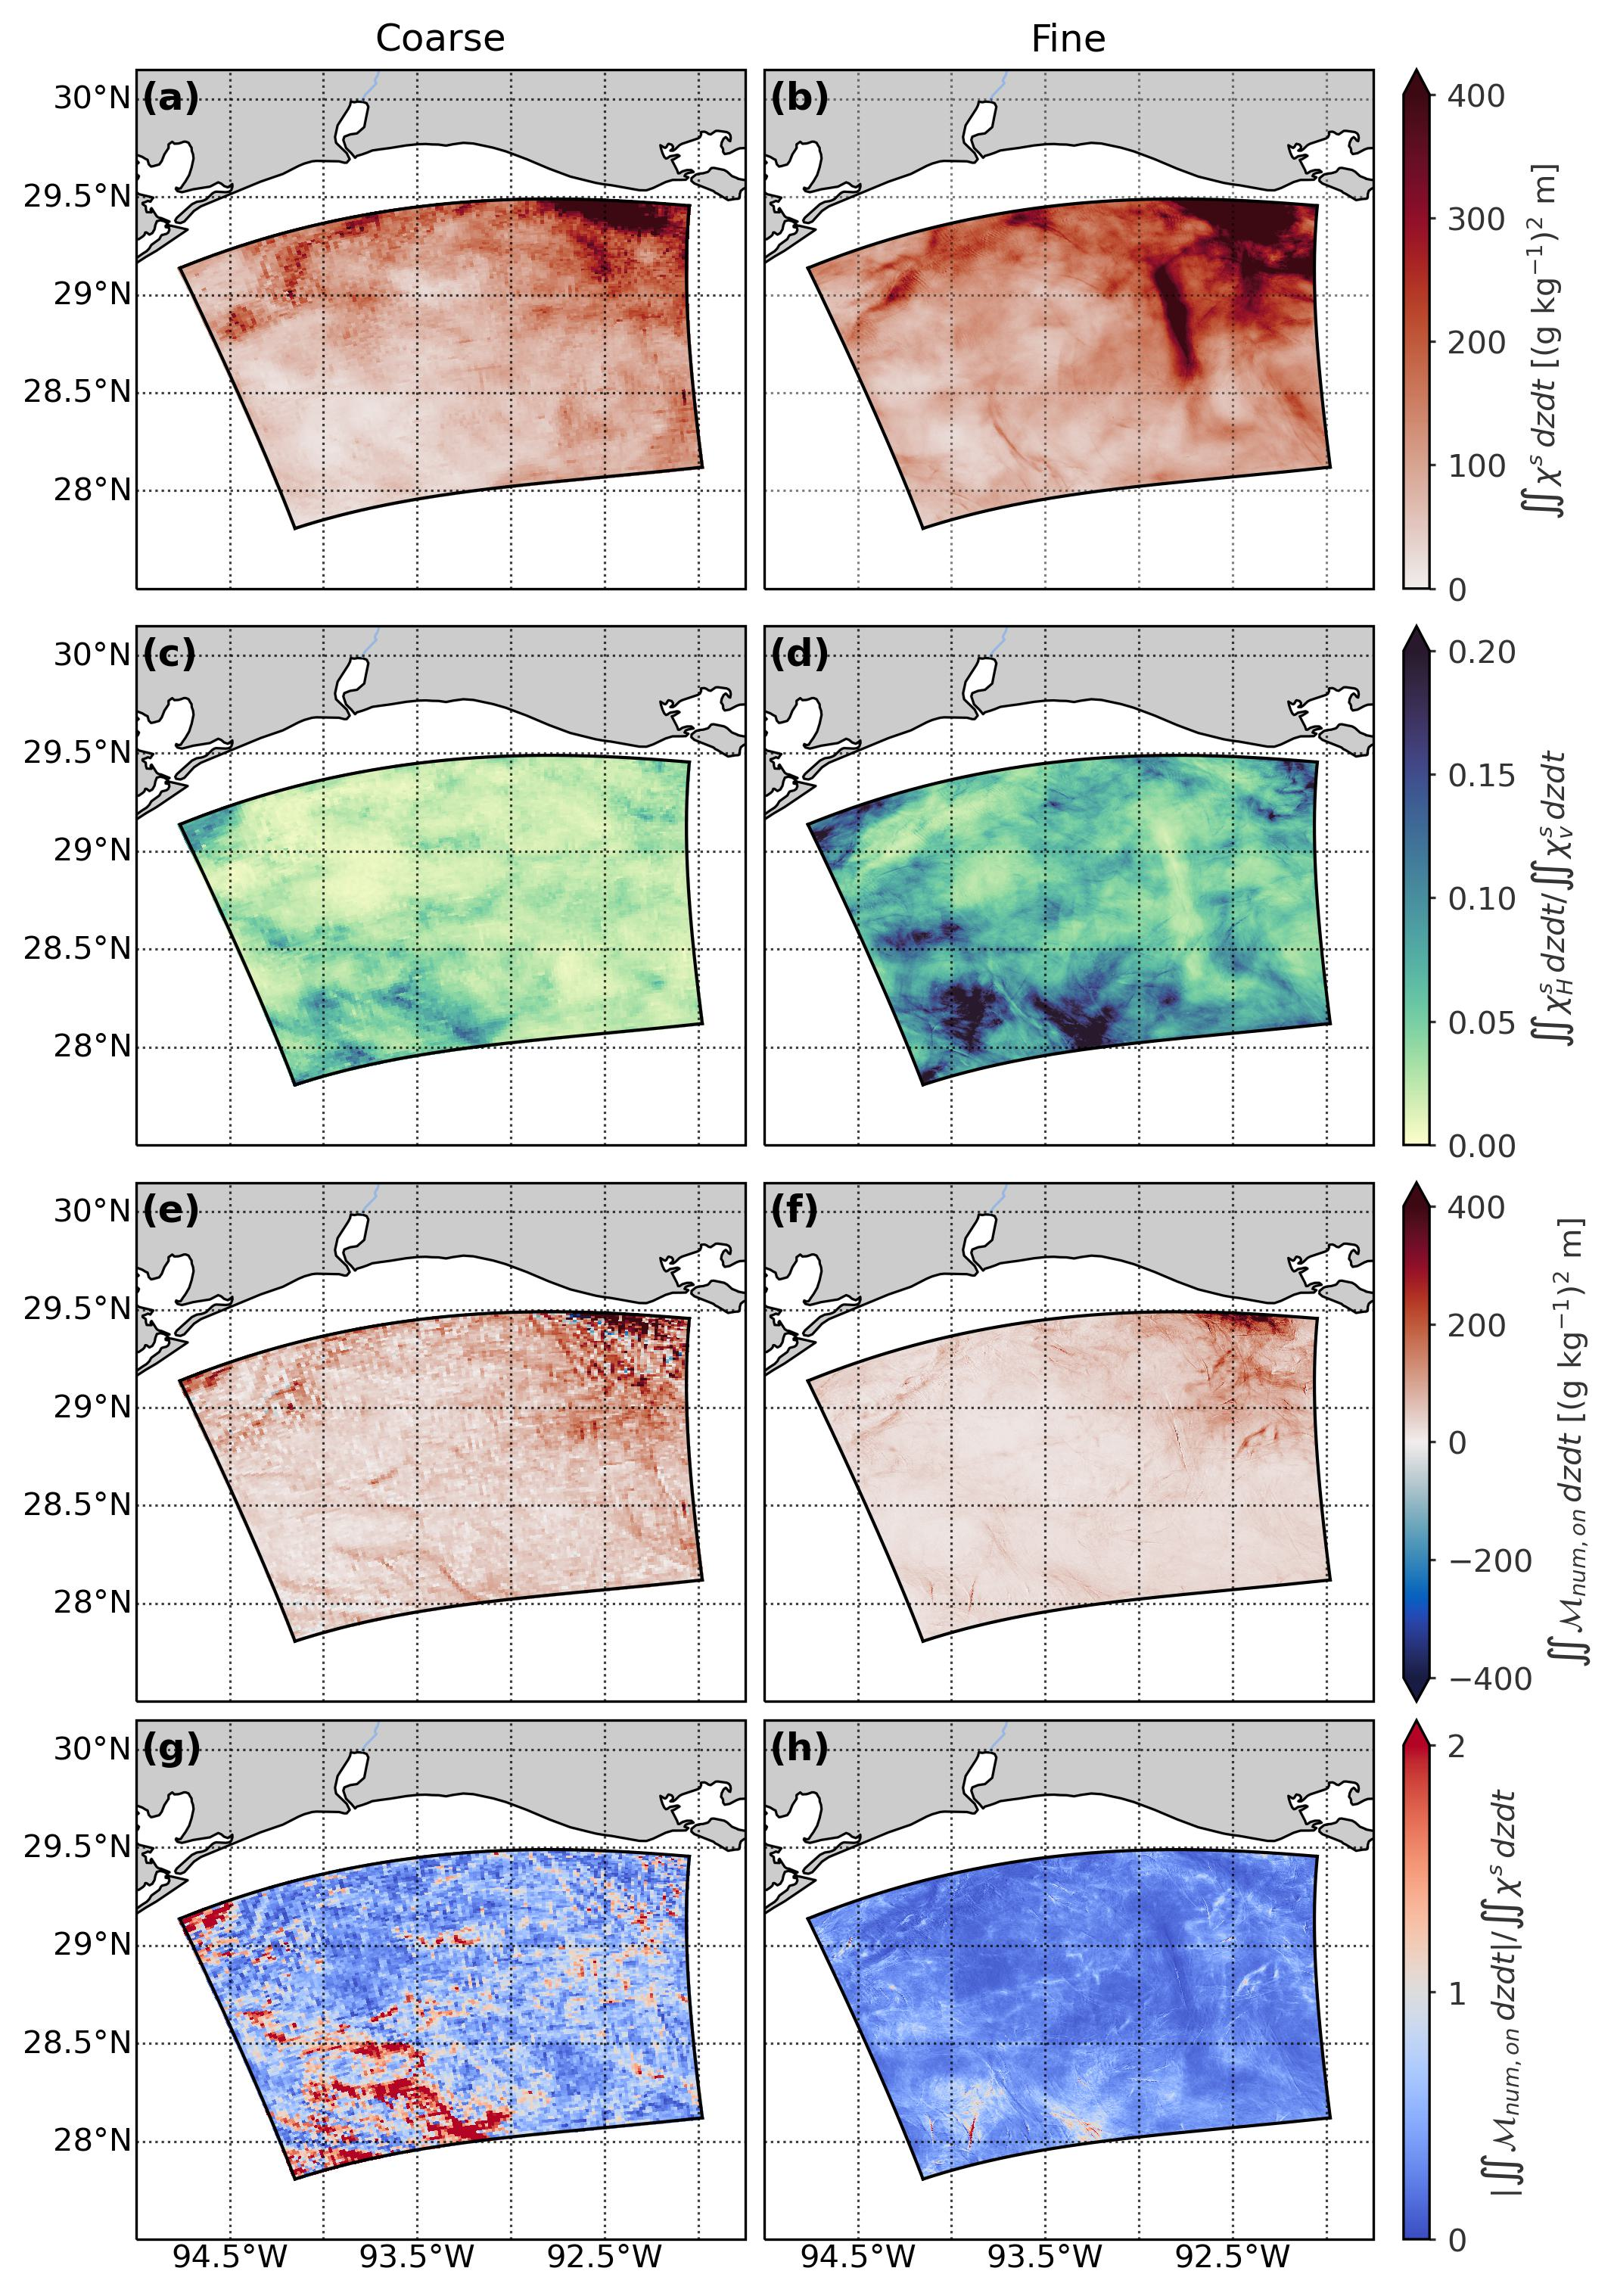
\includegraphics[width = 0.85\linewidth]{figures/james_2023/Figure6_dzdt_int.jpg}}
  \caption{Various depth and time-integrated mixing quantities for the coarse and fine simulations. Depth- and time-integrated total physical mixing $\chi^s$ (a-b). Ratio of depth- and time-integrated $\chi_H^s$ to $\chi_v^s$ (c-d), where bluer colors indicate more horizontal physical mixing and greener colors indicate less horizontal physical mixing. Depth- and time-integrated $\mathcal{M}_{num, on}$ (e-f). Ratio of depth- and time-integrated $\mathcal{M}_{num,on}$ and $\chi^s$ (g-h), where red colors indicate more numerical mixing and blue colors indicate less numerical mixing.}
  \label{fig:depth_integrated}
\end{figure}

\subsection{Temporal variability}

Here, we explore the volume-integrated $s^2$ and $s^{\prime^2}$ budgets and compare the accuracy of the numerical mixing estimated from the $s^{\prime^2}$ budget to the online method. Fig. \ref{fig:budget_comparison} shows a time series for the coarse simulation of surface wind forcing, the terms in Eqs. \ref{eq:salt2_vint} and \ref{eq:svar_int}, and a comparison between the different methods for quantifying volume-integrated numerical mixing. All wind forcing was spatially averaged over the location of the child grid. The land-sea breeze can generally be seen throughout the simulation, with several exceptions (e.g., June 30 and July 7) due to transient wind events such as storms. 

\begin{figure}
 \centerline{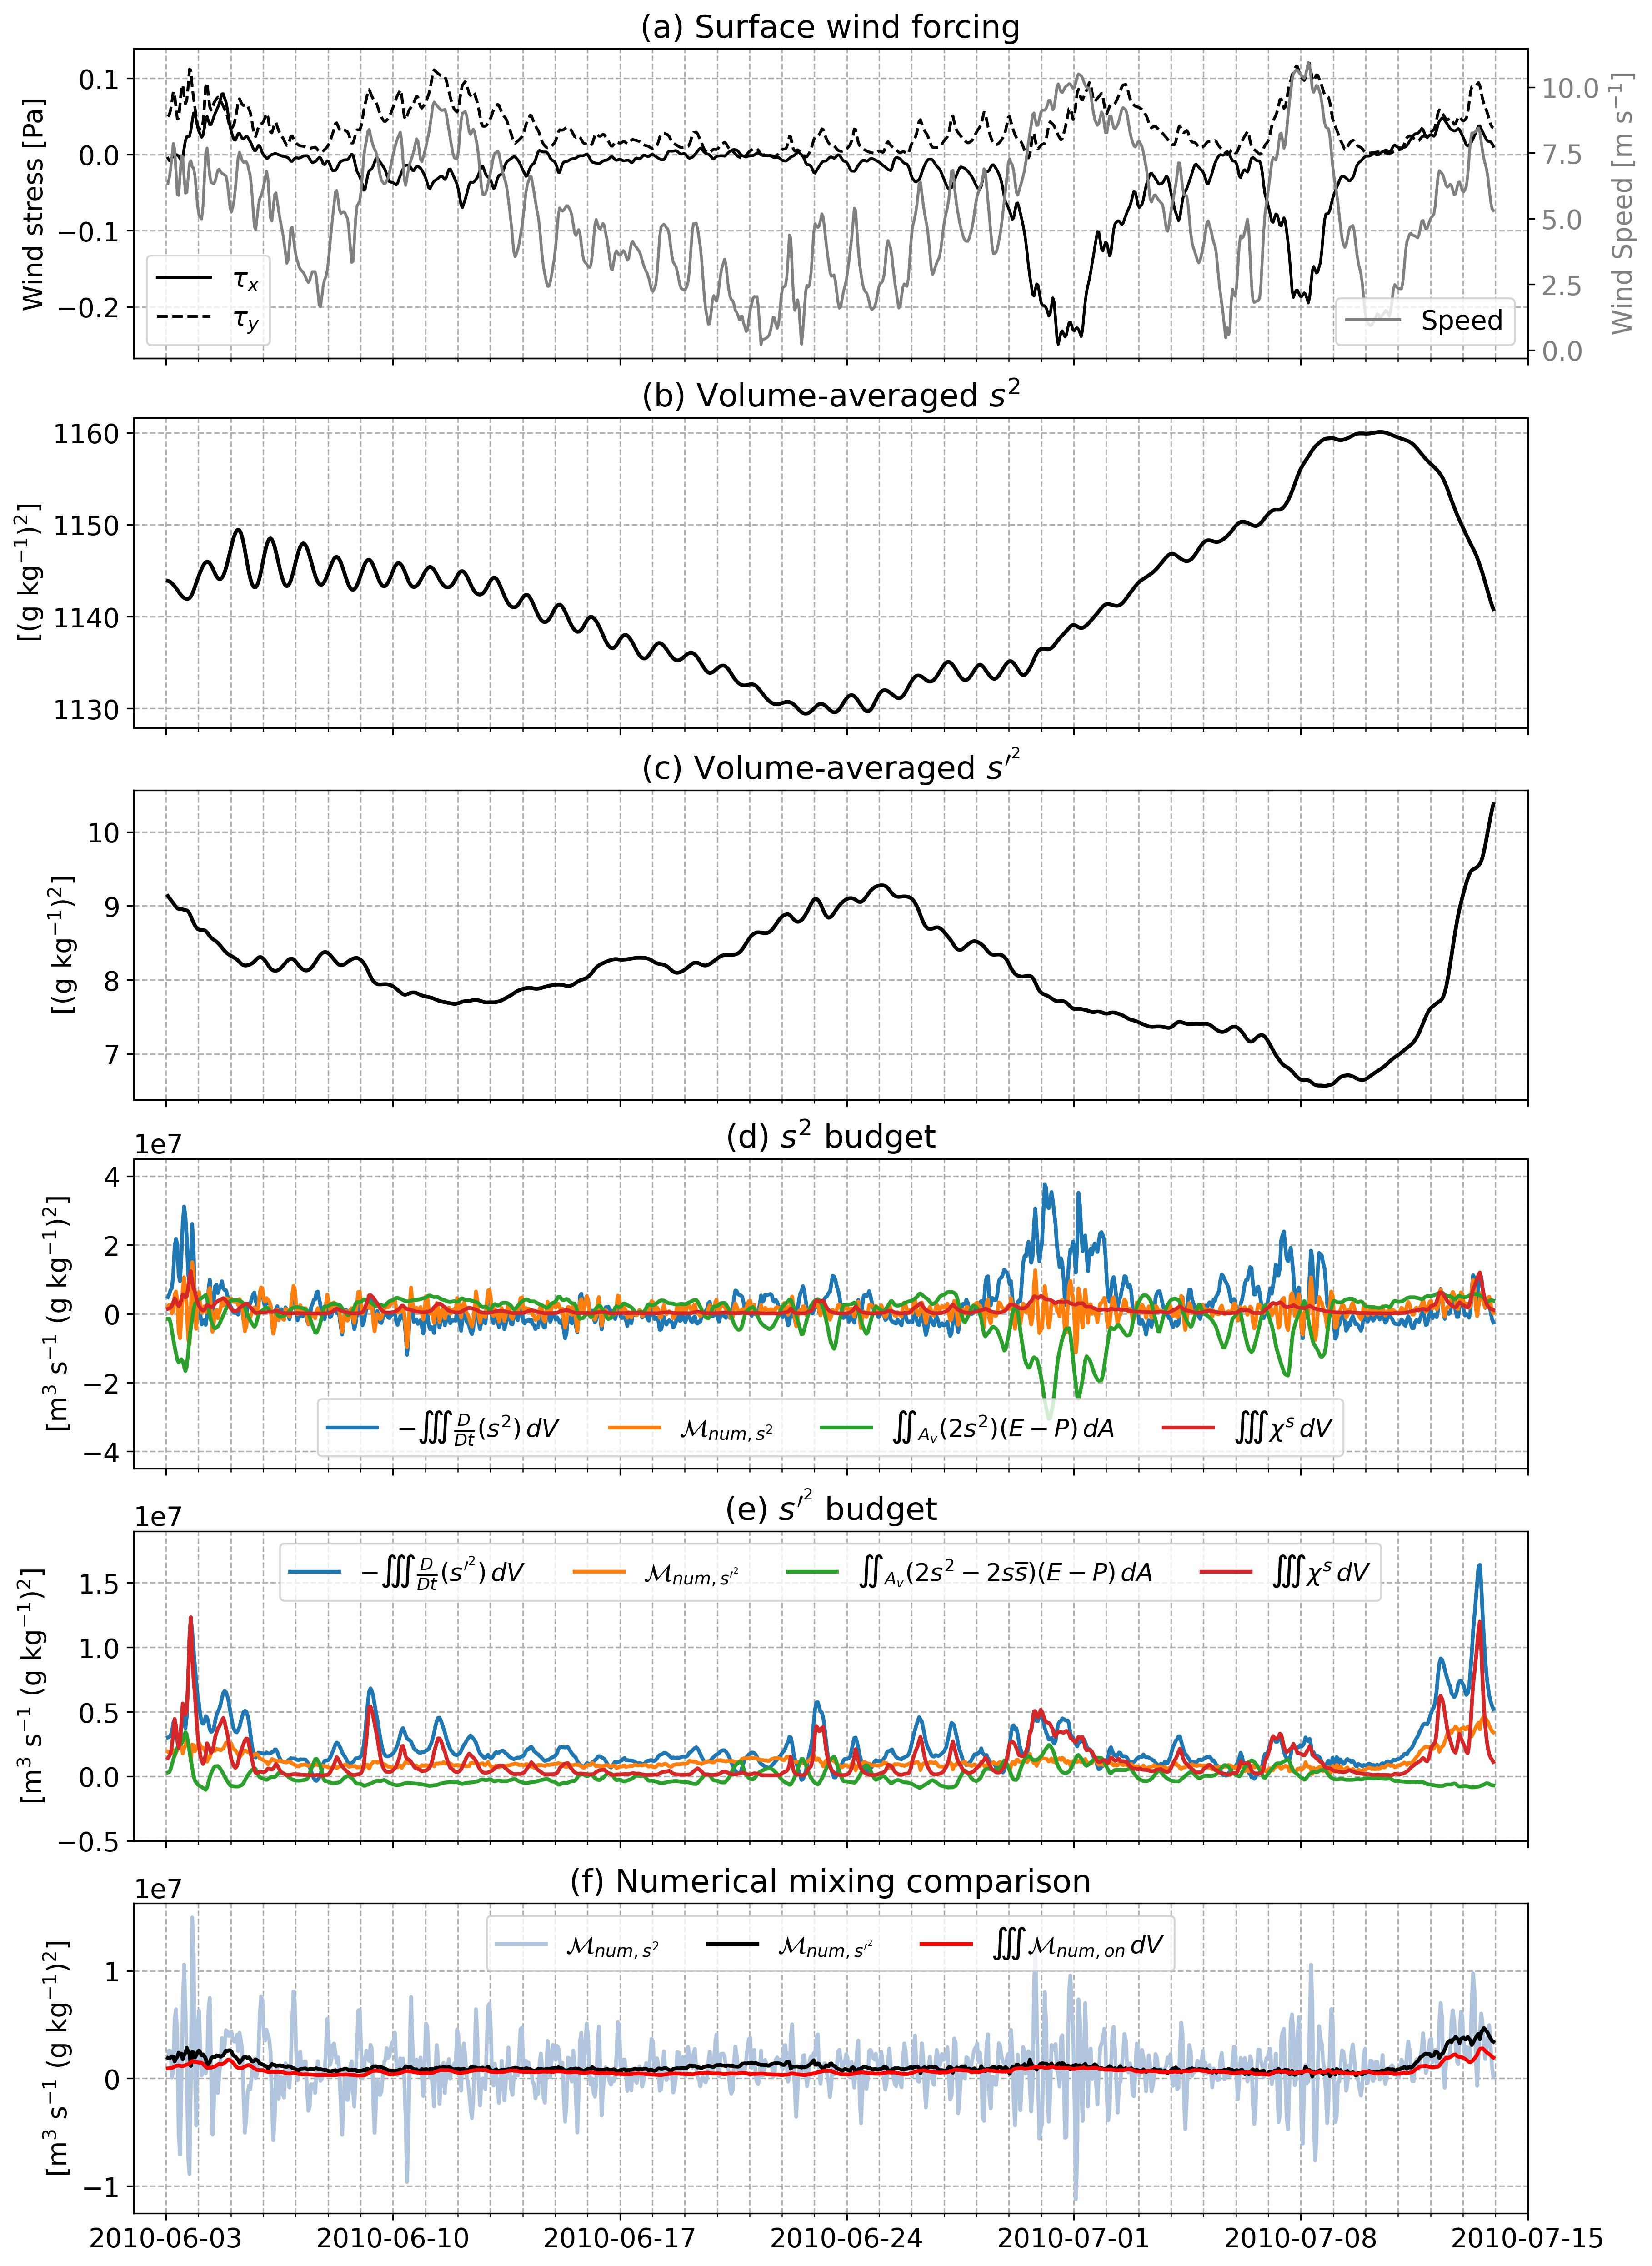
\includegraphics[width = 0.85\linewidth]{figures/james_2023/Figure7_budgets.jpg}}
  \caption{Time series from the coarse simulation averaged over the location of the child grid for east-west wind stress $\tau_x$, north-south wind stress $\tau_y$, and wind speed (a). Volume-averaged $s^2$ (b), volume-averaged $s^{\prime^2}$ (c), volume-integrated $s^2$ budget (d) and $s^{\prime^2}$ budget (e), and comparison between the offline numerical mixing and the online numerical mixing (f). The tendency and advection terms of Eqs. \ref{eq:salt2_vint} and \ref{eq:svar_int} have been combined using the material derivative $\iiint_V \frac{Dc}{Dt} \, dV$, where $c$ denotes the tracer. The horizontal $s^2$ and s$^{\prime^2}$ diffusion terms were omitted from (d) and (e) because they are more than an order of magnitude smaller than the other terms, but are included in their respective numerical mixing calculations.}
  \label{fig:budget_comparison}
\end{figure}

Time series of volume-averaged $s^2$ and $s^{\prime^2}$ (Fig. \ref{fig:budget_comparison} a-b) demonstrate that $s^2\gg s^{\prime^2}$ and that the budgets exhibit a different time dependency. The volume-averaged $s^{\prime^2}$ rarely exceeds $10$ (g kg$^{-1}$)$^2$ and exhibits reduced inertial variability throughout the simulation. The oscillations displayed in the $s^2$ and $s^{\prime^2}$ budgets correspond strongly to the local inertial period ($\sim$ 24 hours) because they are modulated by other variables prone to inertial variability such as the horizontal velocities. Higher frequency oscillations are generated by competition between transient changes in the surface wind field and freshwater input from the M/A rivers. 

For $s^2$ and $s^{\prime^2}$, the advection and tendency terms are highly correlated and have been combined to reduce clutter. Mathematically, this is expressed using the volume integral of their material derivatives and is written as 
\begin{equation}
    \iiint_V \frac{Dc}{Dt} \, dV = \iiint_V \frac{\partial c}{\partial t} \, dV + \iint_{A_l} \mathbf{u}c \cdot \hat{\mathbf{n}} \, dA \quad ,
\end{equation}
 where $c$ is the tracer. Stronger winds are generally associated with larger tendency and advection terms for $s^2$ and $s^{\prime^2}$, which is reflected in their respective material derivatives. The difference between the material derivatives and surface fluxes for $s^2$ and $s^{\prime^2}$ elucidates the influence that removing the volume average salinity has on the dynamics of $s^{\prime^2}$ (Fig. \ref{fig:budget_comparison} c-d). $\iiint \frac{D}{Dt}(s^2) \, dV$ is significantly noisier than $\iiint \frac{D}{Dt}(s^{\prime^2}) \, dV$, which we hypothesize is due the larger numerical error associated with the tendency term, and to a lesser extent, the advection term. The tendency term in the $s^2$ budget is nearly an order of magnitude larger than the $s^{\prime^2}$ budget and will experience larger error because both tendency terms are calculated using the same numerical scheme (i.e., centered finite differences). This error should be reduced by increasing the model output frequency, which we investigate in Section \ref{sec:discussion}. Surface $s^2$ fluxes exert a much larger influence on the $s^2$ budget for much of the simulation, with the physical mixing term often remaining the smallest. The opposite is true for the $s^{\prime^2}$ budget, where the term balance often experiences competition between the physical mixing and the material derivative.  

Estimates of numerical mixing depend strongly on whether $s^2$ or $s^{\prime^2}$ is used, with both offline methods demonstrating significant error with respect to time. $\mathcal{M}_{num, s^2}$ is significantly noisier than $\mathcal{M}_{num, s^{\prime^2}}$ and may exceed the other methods by over an order of magnitude despite the online method being derived in terms of $s$ and $s^2$. Consequently, the $s^2$ budget should not be used for offline quantification of numerical mixing because $\mathcal{M}_{num, s^2}$ does not converge to $\mathcal{M}_{num, s^{\prime^2}}$ for hourly output. $\mathcal{M}_{num, on}$ and $\mathcal{M}_{num, s^{\prime^2}}$ are positive definite, with $\mathcal{M}_{num, s^{\prime^2}}$ almost always overestimating $\mathcal{M}_{num, on}$. The accuracy of $\mathcal{M}_{num, s^{\prime^2}}$ relative to $\mathcal{M}_{num, on}$ is strongly time dependent and the time-averaged $\mathcal{M}_{num, s^{\prime^2}}$ is 60\% larger than the time-averaged $\mathcal{M}_{num, on}$. From June 17-24, the time-averaged $\mathcal{M}_{num, on}$ is 141\% larger than the time-averaged $\mathcal{M}_{num, s^{\prime^2}}$. From July 1-8, however, it is only 12\% larger. These results suggest the offline method is not suitable for accurate quantification of numerical mixing in our model. However, it is unclear whether convergence between $\mathcal{M}_{num, s^2}$, $\mathcal{M}_{num, s^{\prime^2}}$, and $\mathcal{M}_{num,on}$ can be achieved by increasing the output frequency. We discuss possible causes for this, including potential impacts of model output frequency, discretization errors, and other sources of spurious mixing that may contaminate the on- and offline methods in Section \ref{sec:discussion}.  

The effects of the extra terms on the behaviour of the $s^2$ budget are further explored in Fig. \ref{fig:s2_extra_terms}. The volume-averaged salinity changes by less than 1 g kg$^{-1}$ over the simulation and experiences a strong inertial signal until the end of June, after which the inertial signal weakens or vanishes for several days at a time. The differences between the $s^2$ and $s^{\prime^2}$ budgets are generally dominated by competition between $(\partial_t \overline{s}^2)V$ and cross-advective flux $2 \overline{s} \iint (\mathbf{u}s^\prime) \cdot \, dA$ ($r = 0.95$, $p \ll 0.05$). Physically, this relationship shows that in the presence of stratification, the differences between the volume-integrated $s^2$ and $s^{\prime^2}$ budgets is partially modulated by the size of the control volume $V$ ($\partial_t \overline{s}^2$ is small relative to $V$) and the advection of the salinity perturbations through the lateral boundaries. The residual of $(\partial_t \overline{s}^2)V+2 \overline{s} \iint (\mathbf{u}s^\prime) \cdot \hat{\mathbf{n}} \, dA$ is balanced out by the differences in surface fluxes $\iint (2 \overline{s}^2 + 2 \overline{s} s^\prime)(E-P) \, dA$ and the volume-averaged salinity squared times the advection of the flow through the lateral boundaries $\overline{s}^2 \iint \mathbf{u} \cdot \hat{\mathbf{n}} \, dA$. The horizontal cross diffusion term $2 \overline{s} \iiint \nabla_H \cdot (\kappa_H \nabla_H s^{\prime}) \, dV$ remains on average several orders of magnitude smaller than the other terms in the $s^2$ and $s^{\prime^2}$ budgets. This is because the horizontal diffusion terms are small for our model due to prescribed value of $\kappa_H$. Ultimately, all of the extra terms in the $s^2$ budget are linked to $\overline{s}$, with $(\partial_t \overline{s}^2)V$ decreasing in magnitude when amplitude of the inertial variability of $\overline{s}$ decreases. The $\overline{s}^2$ advection term is not as sensitive to the changes in the inertial variability of $\overline{s}$ and oscillates between first and second order, becoming more important at the end of June as $\overline{s}$ begins to increase.

\begin{figure}
 \centerline{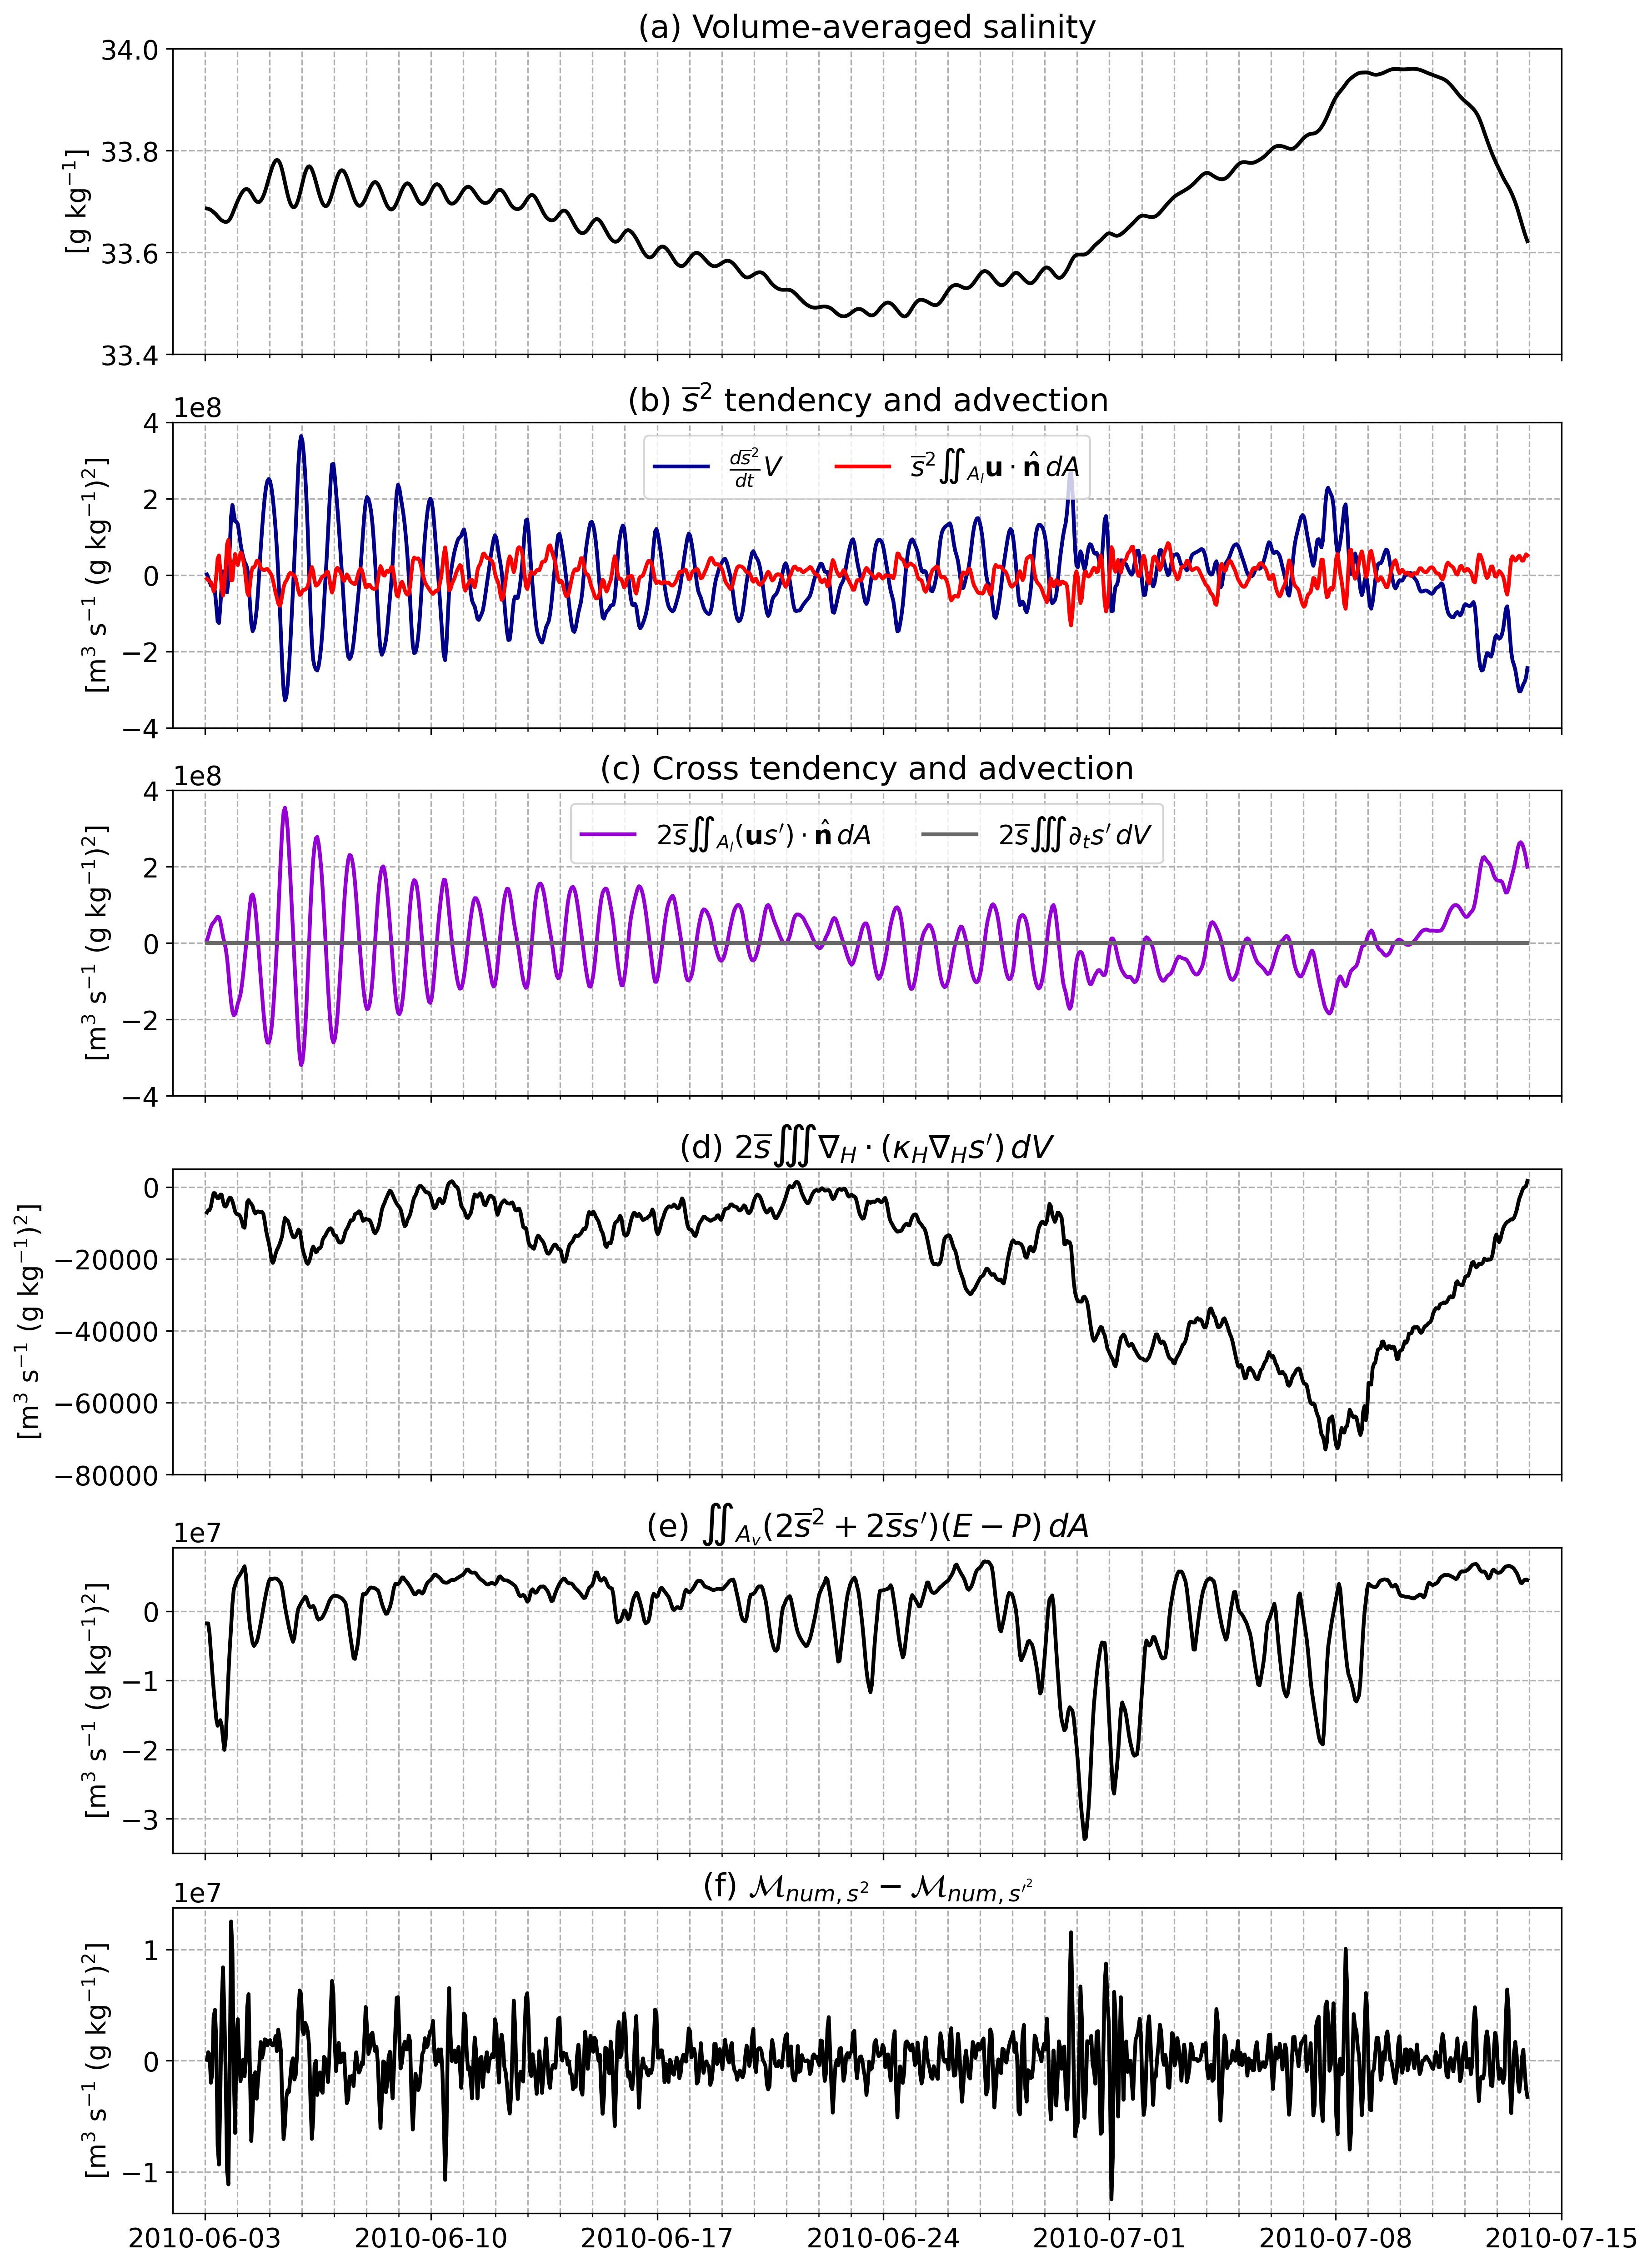
\includegraphics[width = 0.85\linewidth]{figures/james_2023/Figure8_extra_terms.jpg}}
  \caption{Time series from the coarse simulation of the volume-averaged salinity (a) and the balance of the volume-integrated extra terms in the $s^2$ equation given by Eq. \ref{eq:differences}. $\overline{s}^2$ tendency and advection (b), $2 \overline{s} s^\prime$ tendency and advection (c), turbulent horizontal cross diffusion (d), extra $s^2$ surface fluxes (e), and differences between the $s^2$ and $s^{\prime^2}$ numerical mixing $\mathcal{M}_{num, s^2}-\mathcal{M}_{num, s^{\prime^2}}$ (f). $\mathcal{M}_{num, s^2}-\mathcal{M}_{num, s^{\prime^2}}$ yields a large residual that should decrease as model output frequency increases.}
  \label{fig:s2_extra_terms}
\end{figure}

To investigate the bulk impacts of nesting on mixing, Fig. \ref{fig:volume-integrated} displays time series volume-integrated $\chi^s$, $\chi_H^s$, and ratios of fine to coarse $\chi^s$, $\mathcal{M}_{num, on}$, total mixing, and the ratio of $\chi^s$ and $\mathcal{M}_{num, on}$ for both simulations. For the coarse simulation, $\chi_H^s$ comprises 2.3$\%$ of the total physical mixing in the coarse simulation and 5.8$\%$ in the fine simulation. In the coarse simulation, the volume-integrated and time-averaged ratio of numerical to total mixing is 50$\%$. For the fine simulation, this ratio decreases to 32$\%$ because the physical mixing increases and the numerical mixing decreases. The time-averaged physical mixing in the fine simulation is 42$\%$ larger than the coarse simulation and is almost always larger instantaneously, with the greatest disparity occurring during the wind-driven mixing event near July 6 where the fine simulation physical mixing is a factor of four larger than the coarse simulation.  The time-averaged numerical mixing in the fine simulation is 35$\%$ smaller on average relative to the coarse simulation and only grows larger than the coarse numerical mixing at several times. The total mixing in the fine simulation is 14$\%$ larger on average than the coarse simulation, but exhibits large temporal variability and may be twice as large or reduced by a third compared to the coarse simulation. During the first three weeks of June, the total mixing in the fine simulation may be more of less than the coarse simulation due to reduced numerical mixing, but for the remainder of the simulation the relative increase in physical mixing generally exceeds the decrease in numerical mixing. A striking comparison is the ratio of numerical to physical mixing. The numerical mixing is larger than the physical mixing in the coarse simulation for a significant portion of the simulation due to the strong inertial variability in the physical mixing, at several times over half an order of magnitude larger. However, this ratio is significantly reduced in the fine simulation. 

\begin{figure}
 \centerline{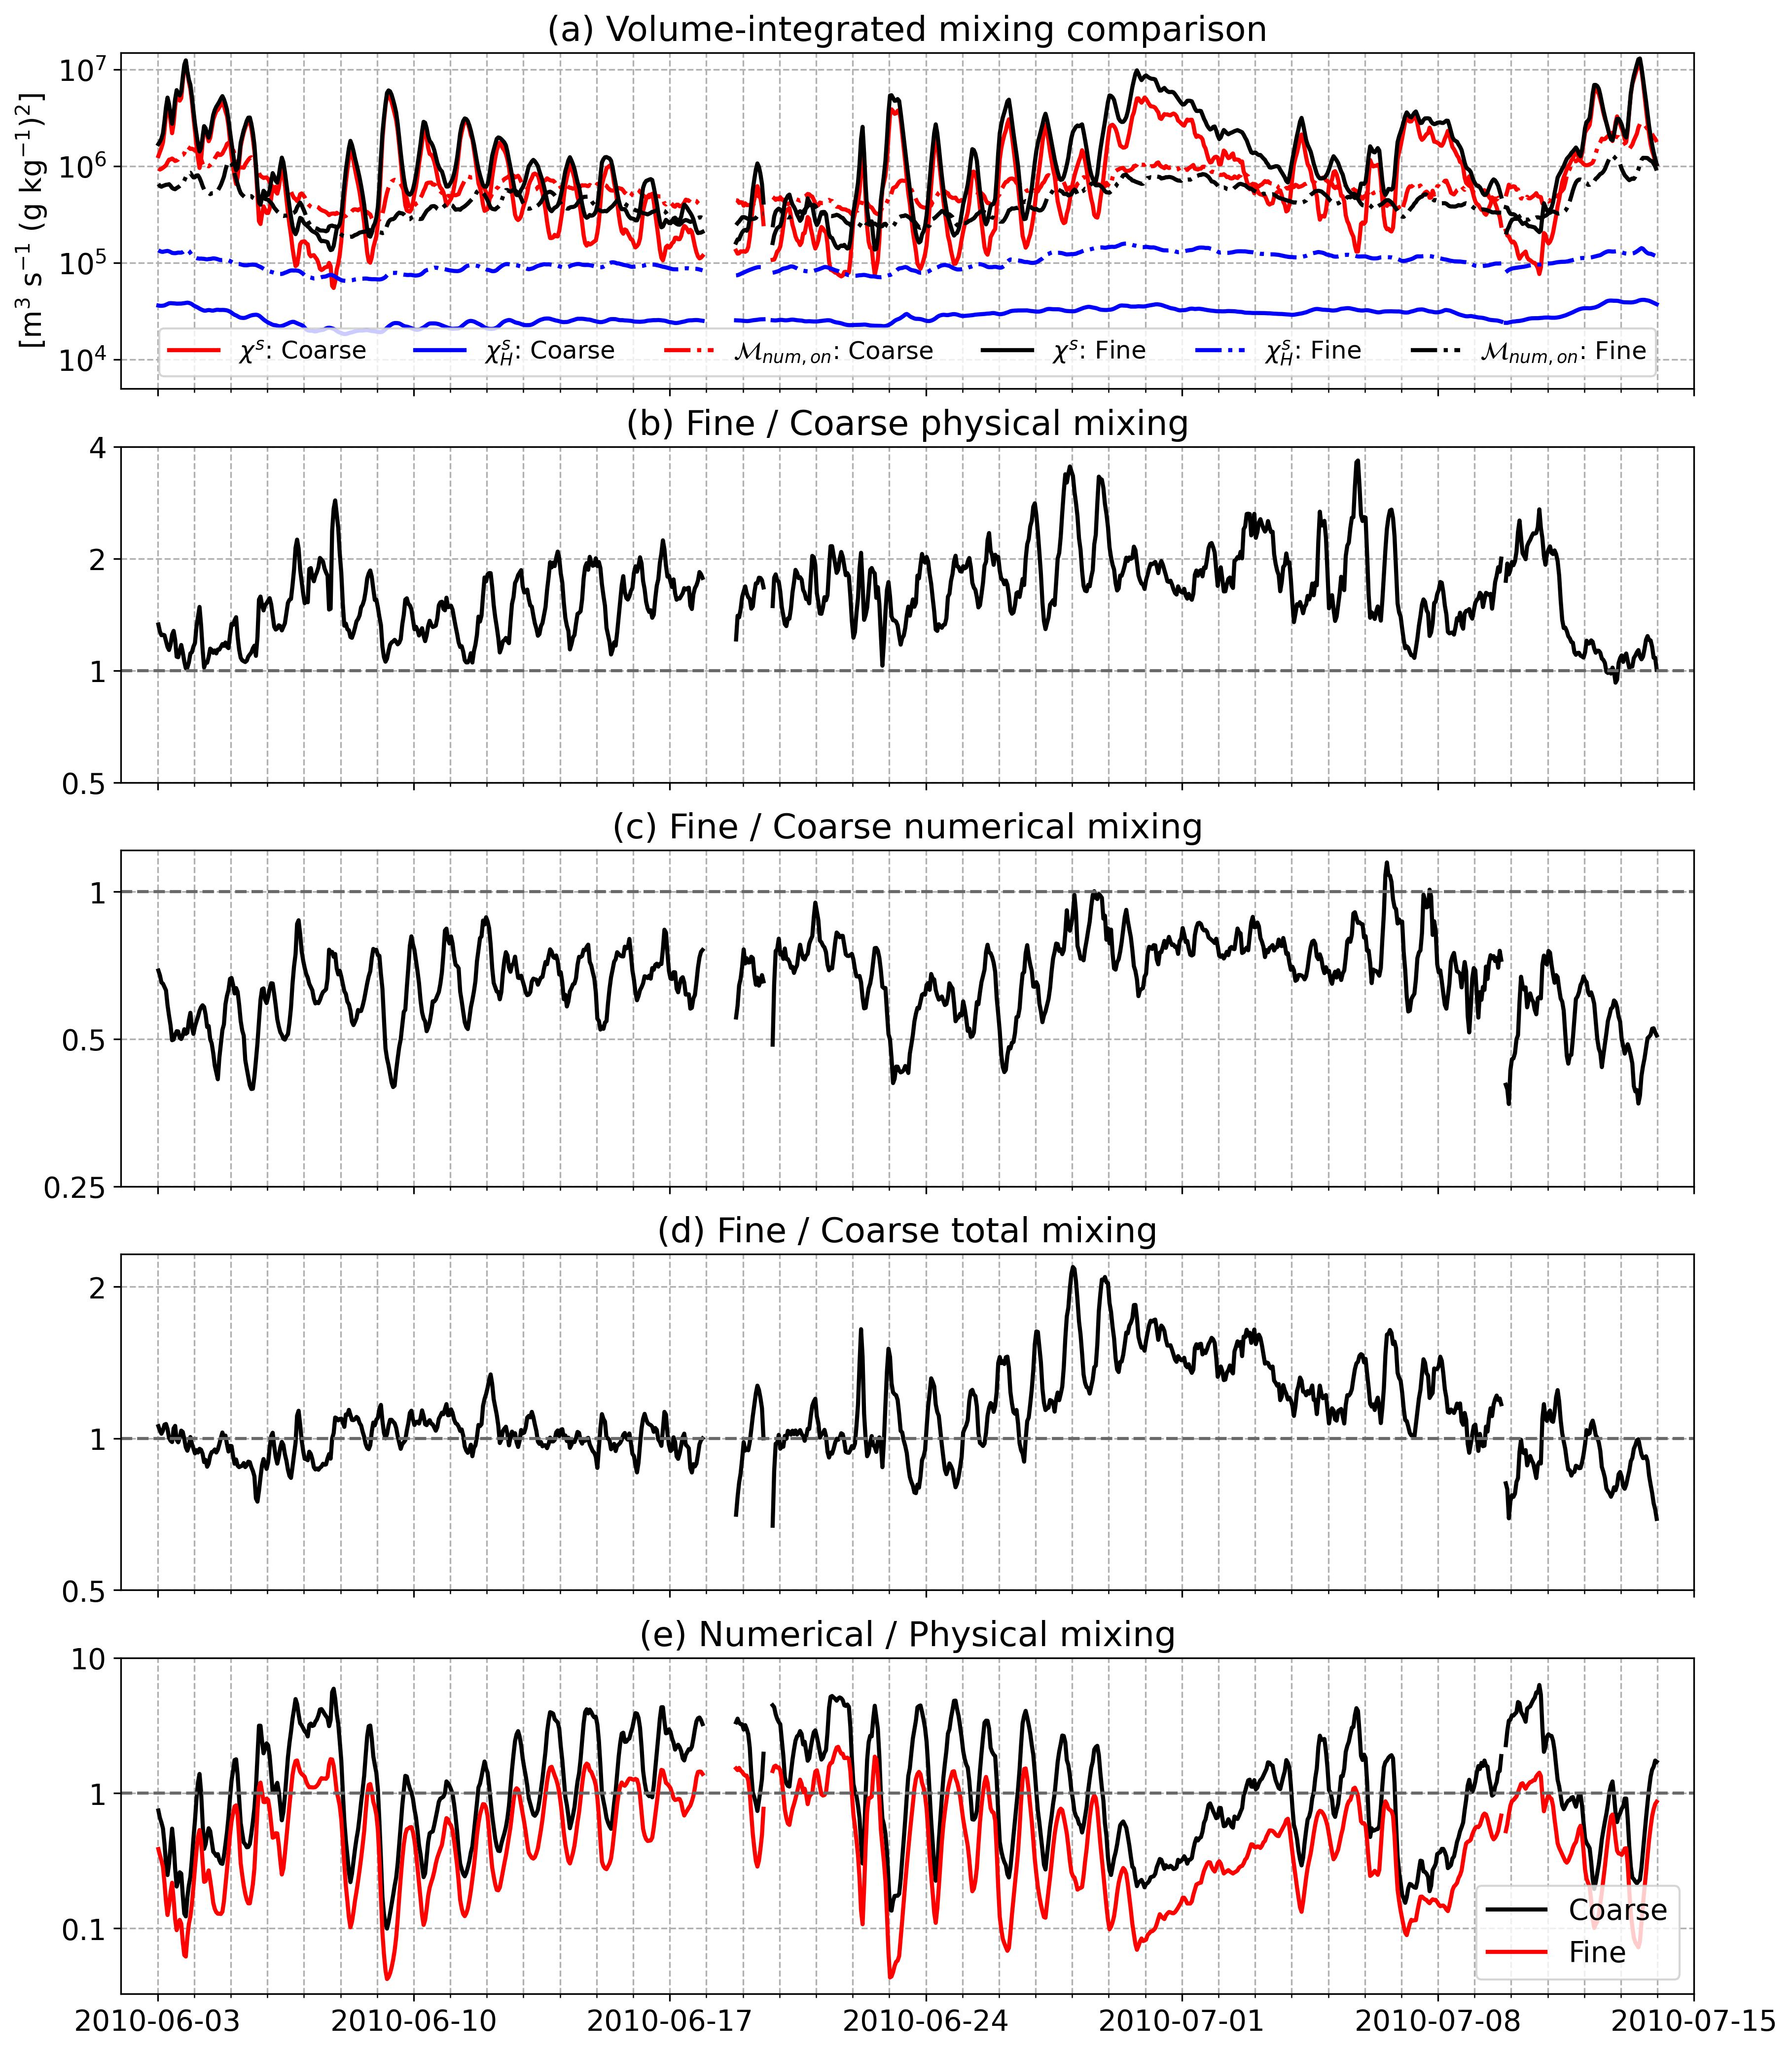
\includegraphics[width = 0.9\linewidth]{figures/james_2023/Figure9_vintegrated.jpg}}
  \caption{Time series of volume-integrated $\chi^s$, $\chi_H^s$,  and $\mathcal{M}_{num, on}$ for the coarse and fine simulations (a). All plots below are derived from these values, displaying fine/coarse physical mixing (b), fine/coarse numerical mixing (c), fine/coarse total mixing (d), and numerical/physical mixing for both models (e). Missing values seen in the time series correspond to output lost during the restart process of the fine simulation and were removed from the parent simulation offline for direct comparison. Note each plot is on a log scale of base 10 or base 2.}
  \label{fig:volume-integrated}
\end{figure}

\section{Discussion} \label{sec:discussion}

We find that numerical mixing constitutes a significant fraction of the total mixing -- the sum of physical and numerical mixing -- and exceeds the physical mixing for much of the simulation due to strong lateral salinity gradients generated by freshwater input from the Mississippi and Atchafalaya rivers.

Our analysis of the offline tracer budgets suggests the $s^2$ budget may overestimate the online numerical mixing by over an order of magnitude (Fig. \ref{fig:budget_comparison}). Building on the work of \citet{Wang_2021}, we hypothesized that the differences are primarily due to errors associated with the tendency term of each tracer and can be reduced by increasing the model output frequency. To test our hypothesis and examine whether $\mathcal{M}_{num, s^2}$ will converge to $\mathcal{M}_{num, s^{\prime^2}}$, we performed two additional numerical simulations of the coarse model with output frequencies of 30- and 10 minutes (twice and six times finer than the native resolution, respectively). The results of the simulations are summarized in Fig. \ref{fig:mixing_time_series} and discussed in Sections \ref{sec:s2_online_conv}-\ref{sec:sprime2_online_conv}.

\begin{figure}[h]
 \centerline{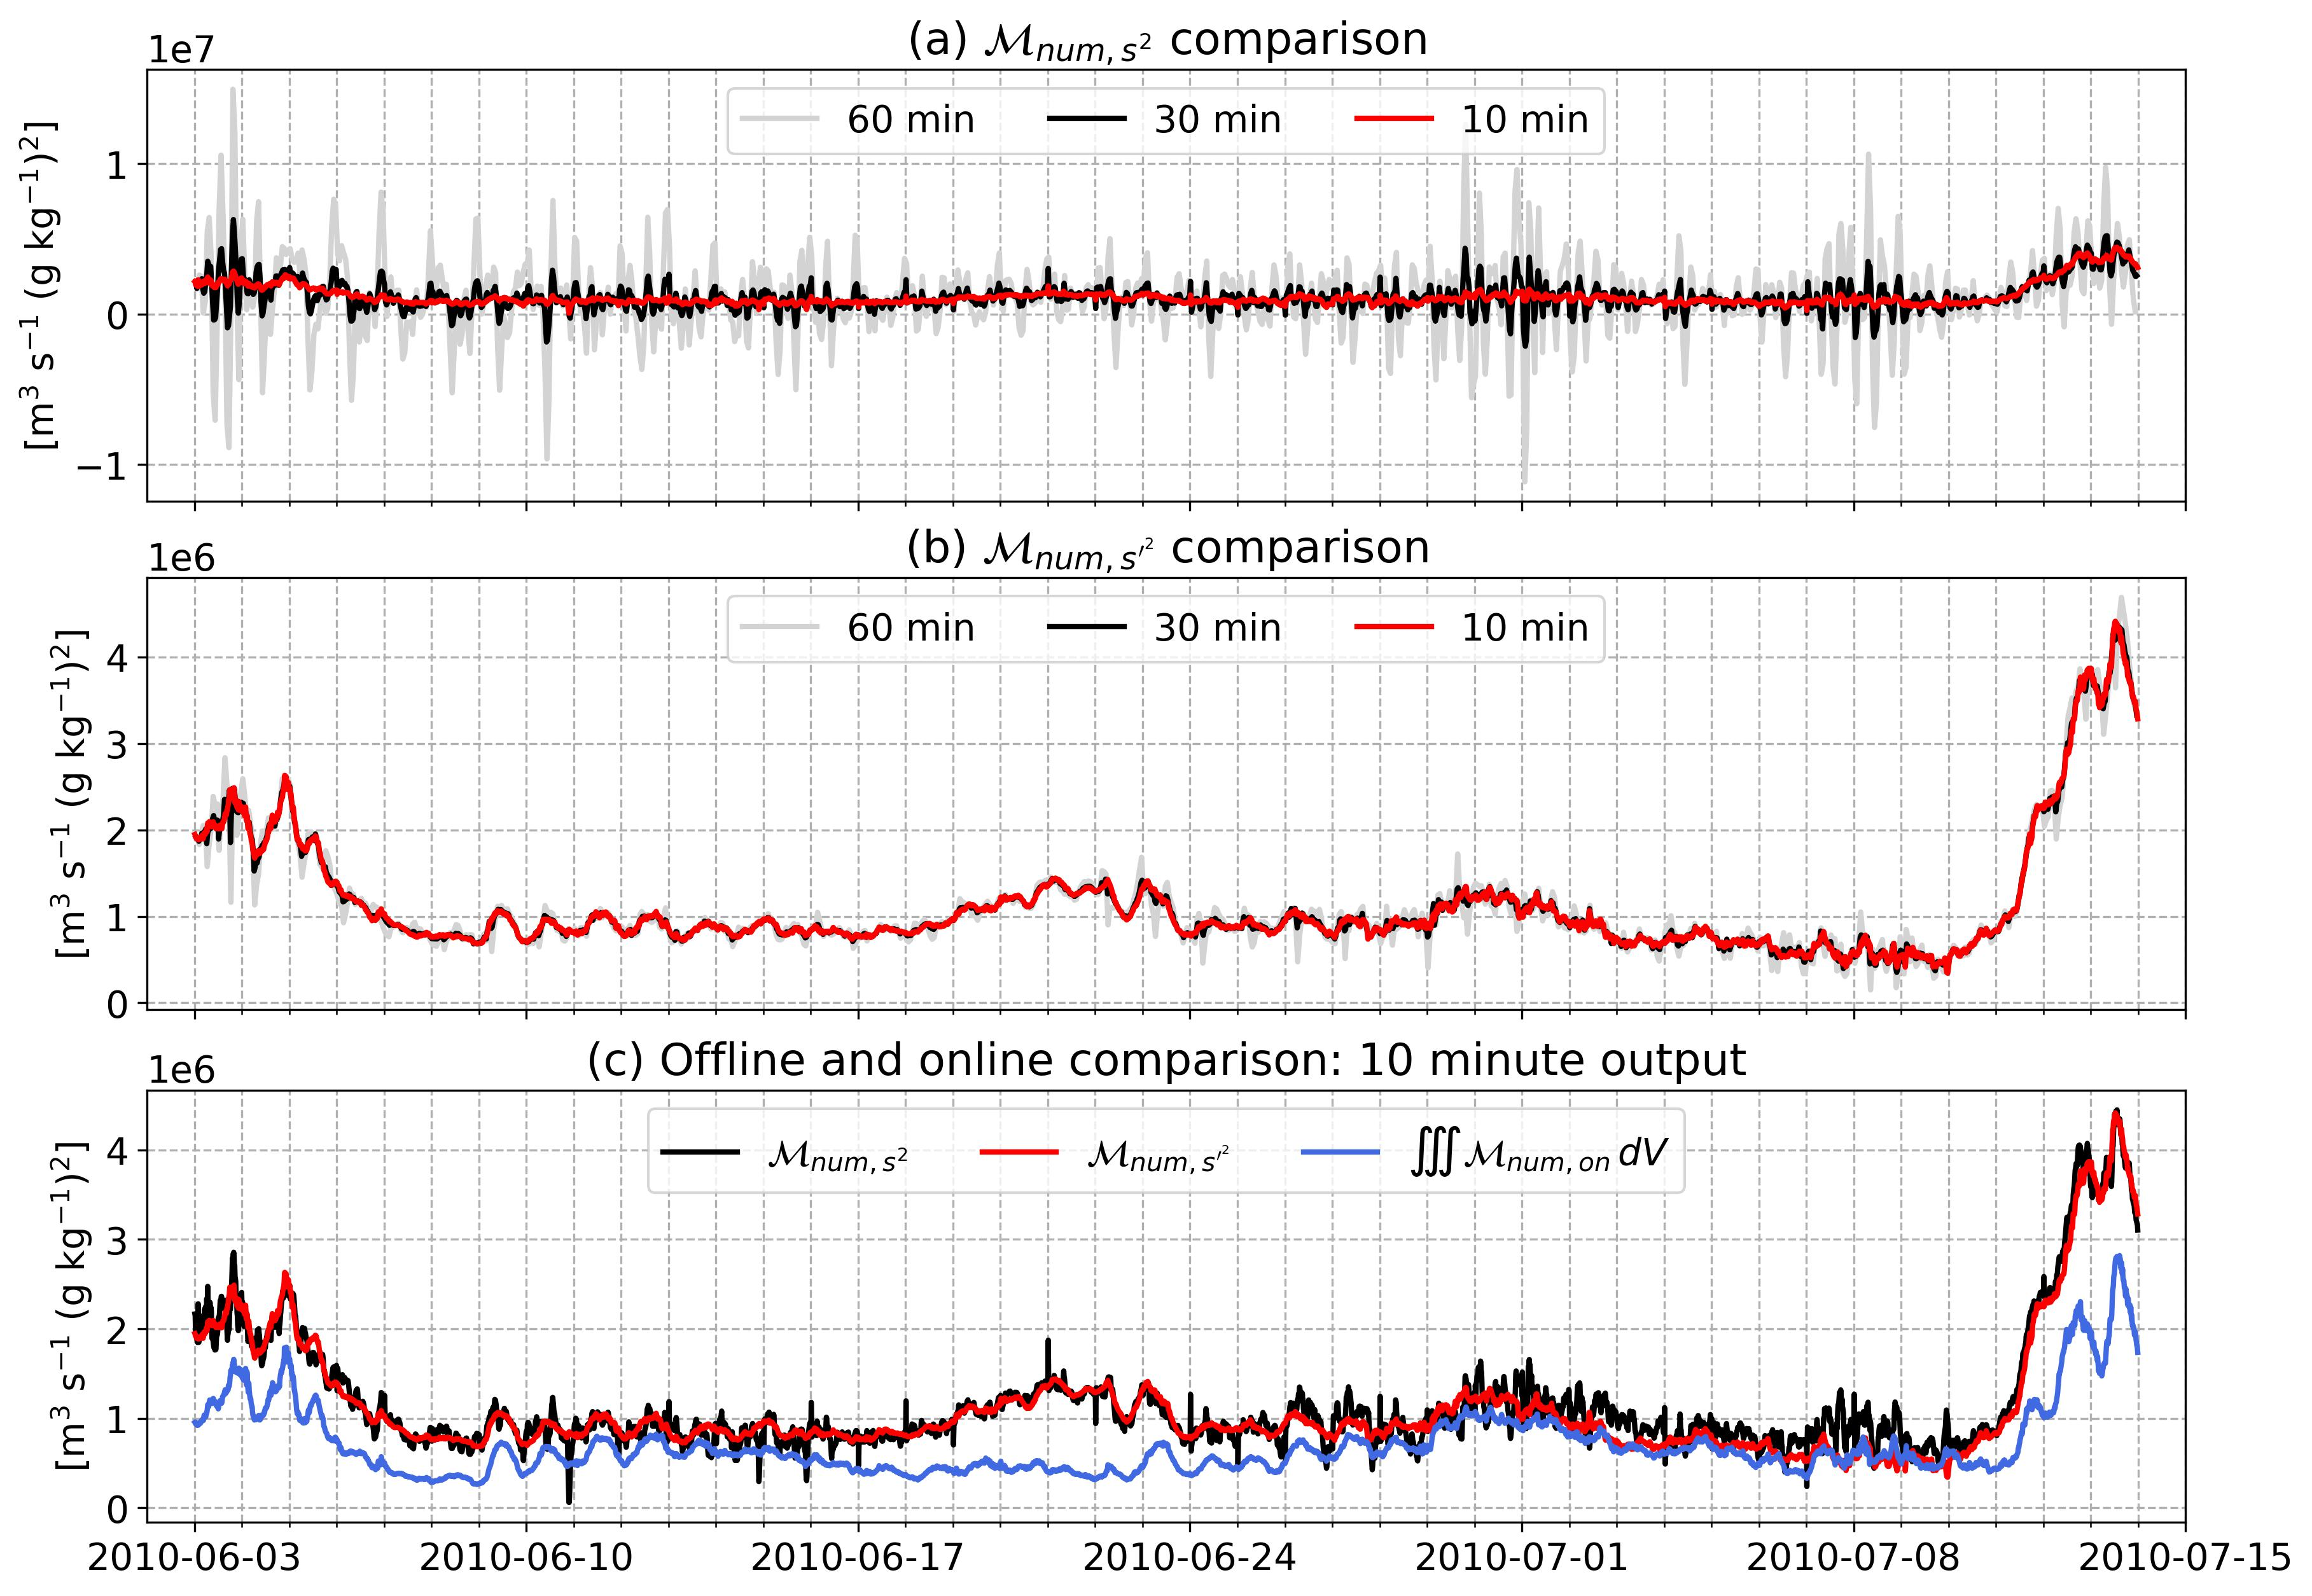
\includegraphics[width = \linewidth]{figures/james_2023/Figure10_output_freq.jpg}}
  \caption{Time series for the coarse simulation for model output frequencies of 60 minutes, 30 minutes, and 10 minutes of $\mathcal{M}_{num, s^2}$ (a) and $\mathcal{M}_{num, s^{\prime^2}}$ (b). Comparison of 10 minute output $\mathcal{M}_{num, s^2}$, $\mathcal{M}_{num, s^{\prime^2}}$, and volume-integrated $\mathcal{M}_{num, on}$  (c).}
  \label{fig:mixing_time_series}
\end{figure}

Additionally, the local and volume-integrated numerical mixing constitute significant fractions of the total mixing, even when the model resolution is increased to $\mathcal{O}(300)$ m in a two-way nested simulation. Despite the time-averaged spatially-integrated numerical mixing decreasing in the fine simulation by 35\%, Fig. \ref{fig:cross_section} suggests that numerical mixing may be occasionally enhanced at the grid-scale. Numerical mixing is dependent on a number of factors, including the magnitude of the horizontal salinity gradients, grid resolution, model timestep, and the representation of dynamical processes. \citet{Wang_2021} suggested that numerical mixing is proportional to the square of the horizontal salinity gradients, however they did not demonstrate that this relationship is robust for higher order and more complex advection schemes. We find, based on Figs.~\ref{fig:surface_pdfs} and~\ref{fig:whole_pdfs} that, on average, the salinity gradients do not increase significantly in the fine simulation, but there are more instances of high values of relative vorticity, divergence, and strain. Even when considering the increased horizontal mixing in the fine simulation, the results suggest that different physical processes have emerged in the fine simulation. We discuss the relationship between horizontal resolution, numerical mixing, and model processes in Section \ref{sec:salinity_gradient_mag}. 

\subsection{Convergence between $\mathcal{M}_{num, s^2}$ and $\mathcal{M}_{num, s^{\prime^2}}$}
\label{sec:s2_online_conv}

As the output frequency increases, $\mathcal{M}_{num,s^2}$ beings to converge towards $\mathcal{M}_{num,s^{\prime^2}}$ but still remains noisy, with the two in much better agreement for the 10 minute output simulation. However, we find this insufficient because 10 minute output is impractical for long-term coastal ocean simulations at this time. To test our hypothesis that the higher inaccuracy associated with $\mathcal{M}_{num, s^2}$ is primarily due to errors associated with the tendency term $\iiint_V \partial_t s^2 \, dV$, we down-sampled the 10 minute output of the $s^2$ budget to match the 30 minute output. After rearranging Eq. \ref{eq:salt2_vint}, the residual term balance can be written as 
\begin{equation} \label{eq:downsampled_termbalance}
    \begin{split}
    \Delta \mathcal{M}_{num, s^2} = -\Delta \textrm{Tendency}-\Delta \textrm{Advection}+\Delta \textrm{Surface $s^2$ flux}-\Delta \textrm{Physical mixing} \\
    + \Delta \textrm{Horz. diff.} \quad ,
    \end{split}
\end{equation}
where $\Delta = \gamma_{30}-\gamma_{10}$, with $\gamma$ denoting the terms in the volume-integrated $s^2$ budget and the subscripts referring to the model output frequency in minutes. The difference in the estimate of numerical mixing due to differences in model output frequency is given by $\Delta \mathcal{M}_{num, s^2}$. 

We computed the covariance between each term in Eq. \ref{eq:downsampled_termbalance} and $\Delta \mathcal{M}_{num, s^2}$ divided by the variance of $\Delta \mathcal{M}_{num, s^2}$ to test the significance of each term, which we denote by the variable $q$. This provides an estimate of the fraction of the variance in $\Delta \mathcal{M}_{num, s^2}$ explained by each term. For $-\Delta$Tendency, $q = 1.271$ and for $-\Delta$Advection, $q = -0.270$, indicating that $\Delta$Tendency will over-predict $\Delta \mathcal{M}_{num, s^2}$, whereas $-\Delta$Advection will compensate for this over-prediction. When combined, $q = 1.001$, indicating that $\Delta$Physical Mixing, $\Delta$Surface flux, and $\Delta$Horz. Diff. do not significantly contribute to $\Delta \mathcal{M}_{num, s^2}$, which is because they are orders of magnitude smaller relative to $\Delta$Tendency and $\Delta$Advection. $\Delta$Advection is also significant, but to a lesser extent than $\Delta$Tendency because the horizontal velocities are highly unsteady and therefore sensitive to model output frequency. The physical mixing is computed online and remains more periodic relative to $\Delta$Tendency and $\Delta$Advection, so it is less sensitive to model output frequency. Likewise, the freshwater flux $(E-P)$ has an temporal resolution of several hours that is linearly interpolated prior to the calculation of $\Delta$Surface flux, so it is unsurprising it remains insignificant. $\Delta$Horz. diff. does not change signficantly because the horizontal $s^2$ diffusion is well under an order of magnitude smaller than the other terms in the volume-integrated $s^2$ budget. These results were consistent with scatter plots of $\Delta \mathcal{M}_{num, s^2}$ and the RHS terms of Eq. \ref{eq:downsampled_termbalance} (not shown). 

\subsection{Convergence between $\mathcal{M}_{num,s^{\prime^2}}$ and $\mathcal{M}_{num,on}$}
\label{sec:sprime2_online_conv}

For 10 minute output, $\mathcal{M}_{num,s^{\prime^2}}$ becomes slightly less noisy but the general structure remains unchanged and unconditional convergence (i.e., for all times) is not achieved. Interestingly, convergence does not substantially improve as output frequency increases, especially during the last week of the simulation when the largest physical and numerical mixing occurs (Fig. \ref{fig:budget_comparison} d). 

There are a number of factors that could cause the difference between on- and offline estimates of numerical mixing, and many of them are difficult to quantify. First, we cannot say with certainty that $\mathcal{M}_{num, on}$ will yield identical results whether $s$ or $s^{\prime}$ is computed locally despite our analysis with a 1D upwind scheme. Another source of error is our use of lower-order accurate discretizations for offline analysis of the tracer variance budgets (see \ref{Appendix:offline_method}). For example, ROMS has implemented several higher order internal time-stepping schemes for tracers since its inception (e.g., third-order Adams-Bashforth), whereas we use a first order centered finite difference for time derivatives in the $s^2$ and $s^{\prime^2}$ budgets. Likewise, we used volume-conserving fluxes in the calculation of the $s^2$ and $s^{\prime^2}$ boundary advection instead of reconstructing the MPDATA scheme offline. These discretization errors may be further compounded by our use of average files compared to snapshots.

The reason for this is the offline method is intended to focus on practicality. Recreating a model's complex numerical schemes offline may be more cumbersome than coding the online method into the source code and rerunning it if computational resources are not a concern. Other sources of error are the numerical diffusion of $s^2$ and $s^{\prime^2}$ through the lateral boundaries of the control volume or the generation of spurious convection. Quantification of numerical diffusion would require estimating a numerical diffusion coefficient and as we have shown, we cannot guarantee an offline calculation will be robust. The situation is similar regarding the quantification of spurious convection. 

The online method should be used as the reference due to the lack of convergence and influence of discretization errors associated with the offline method. We can say that increasing the model output frequency will marginally improve the offline estimates, and that the $s^{\prime^2}$ budget will generally yield more accurate estimates of the numerical mixing than the $s^2$ budget, especially at low output frequency. In our case, $\mathcal{M}_{num, s^{\prime^2}}$ almost always overestimates $\mathcal{M}_{num, on}$ and qualitatively captures the temporal variability well. However, there is no guarantee this will be the case for other ocean models. Therefore, we cannot recommend the offline method for generic analysis of numerical mixing because it does not converge even at impractically-high output frequencies and we are unable to identify the exact reasons for the lack of convergence. These issues may be compounded for larger-scale ocean models. The proper output variables would have to be chosen before running the simulation and the output frequency will be decreased for larger-scale models. Future research could potentially improve the offline method by using more higher-order numerical schemes for the tendency and advection terms, but this would have to be tested on a per-model basis and referenced against an online benchmark for validation.

\subsection{Relating numerical mixing to $|\nabla_H s|$ and other processes} \label{sec:salinity_gradient_mag}

As shown in Fig. \ref{fig:cross_section}, numerical mixing may be over an order of magnitude larger than the physical mixing in regions with strong density gradients, generally corresponding to areas of larger $|\nabla_H s|$. \citet{Smolarkiewicz_1983} showed that after discretizing a one-dimensional advection equation with a first-order upwind scheme, the numerical mixing $\mathcal{M}_{num, up}$ is
\begin{equation} \label{eq:mnum_approx}
    \mathcal{M}_{num, up} = |u|\Delta x (1-C) \bigg(\frac{\partial s}{\partial x} \bigg)^2 \sim |u|\Delta x \bigg(\frac{\partial s}{\partial x} \bigg)^2 \quad ,
\end{equation}
where $|u|$ is the magnitude of the constant horizontal velocity, $\Delta x$ is the horizontal grid resolution, $C=\frac{u \Delta t}{\Delta x}$ is the Courant number with online time step $\Delta t$. After rearranging, it can be shown that the right-hand-side of Eq. \ref{eq:mnum_approx} is formulated such that the numerical mixing is equal to an implicit diffusion coefficient $|u|\Delta x-u^2 \Delta t$ multiplied by the square of the horizontal salinity gradients. As \citet{Wang_2021} notes, when the Courant number is less than one, the numerical mixing is approximately proportional to the square of the horizontal salinity gradients. \citet{Wang_2021} applied this equation to a realistic simulation of the Changjiang River plume using two tracer advection schemes (MPDATA and Third-order Upstream-biased Horizontal Scheme) and suggested that this relationship holds true qualitatively (their Figs. 8-9). 

We further investigate the relationship between $\mathcal{M}_{num, on}$ and $(\nabla_H s)^2 = (\partial_x s)^2+(\partial_y s)^2$ in Fig. \ref{fig:mnum_sgrad}, which shows weighted histograms of the absolute value of $\mathcal{M}_{num, on}$ and $(\nabla_H s)^2$ in log$_{10}$ space, weighted by grid cell volume $dV$, for the coarse and fine simulations. We performed a weighted linear regression analysis to test the robustness of the two-dimensional form of Eq. \ref{eq:mnum_approx}. There is a clear log-log relationship between $\mathcal{M}_{num, on}$ and $(\nabla_H s)^2$ ($r^2=0.55$ for coarse simulation, $r^2=0.39$ for the fine simulation). To test for a power law dependence, we conducted an empirical linear fit of $\mathcal{M}_{num, on}$ and $(\nabla_H s)^2$ in log$_{10}$ space, which slightly improved the fit ($r^2=0.60$ for coarse simulation, $r^2=0.46$ for the fine simulation). The relatively high $r^2$ suggest that the horizontal salinity gradients could be used to roughly approximate the numerical mixing, even for higher order and more complex advection schemes.

\begin{figure}
 \centerline{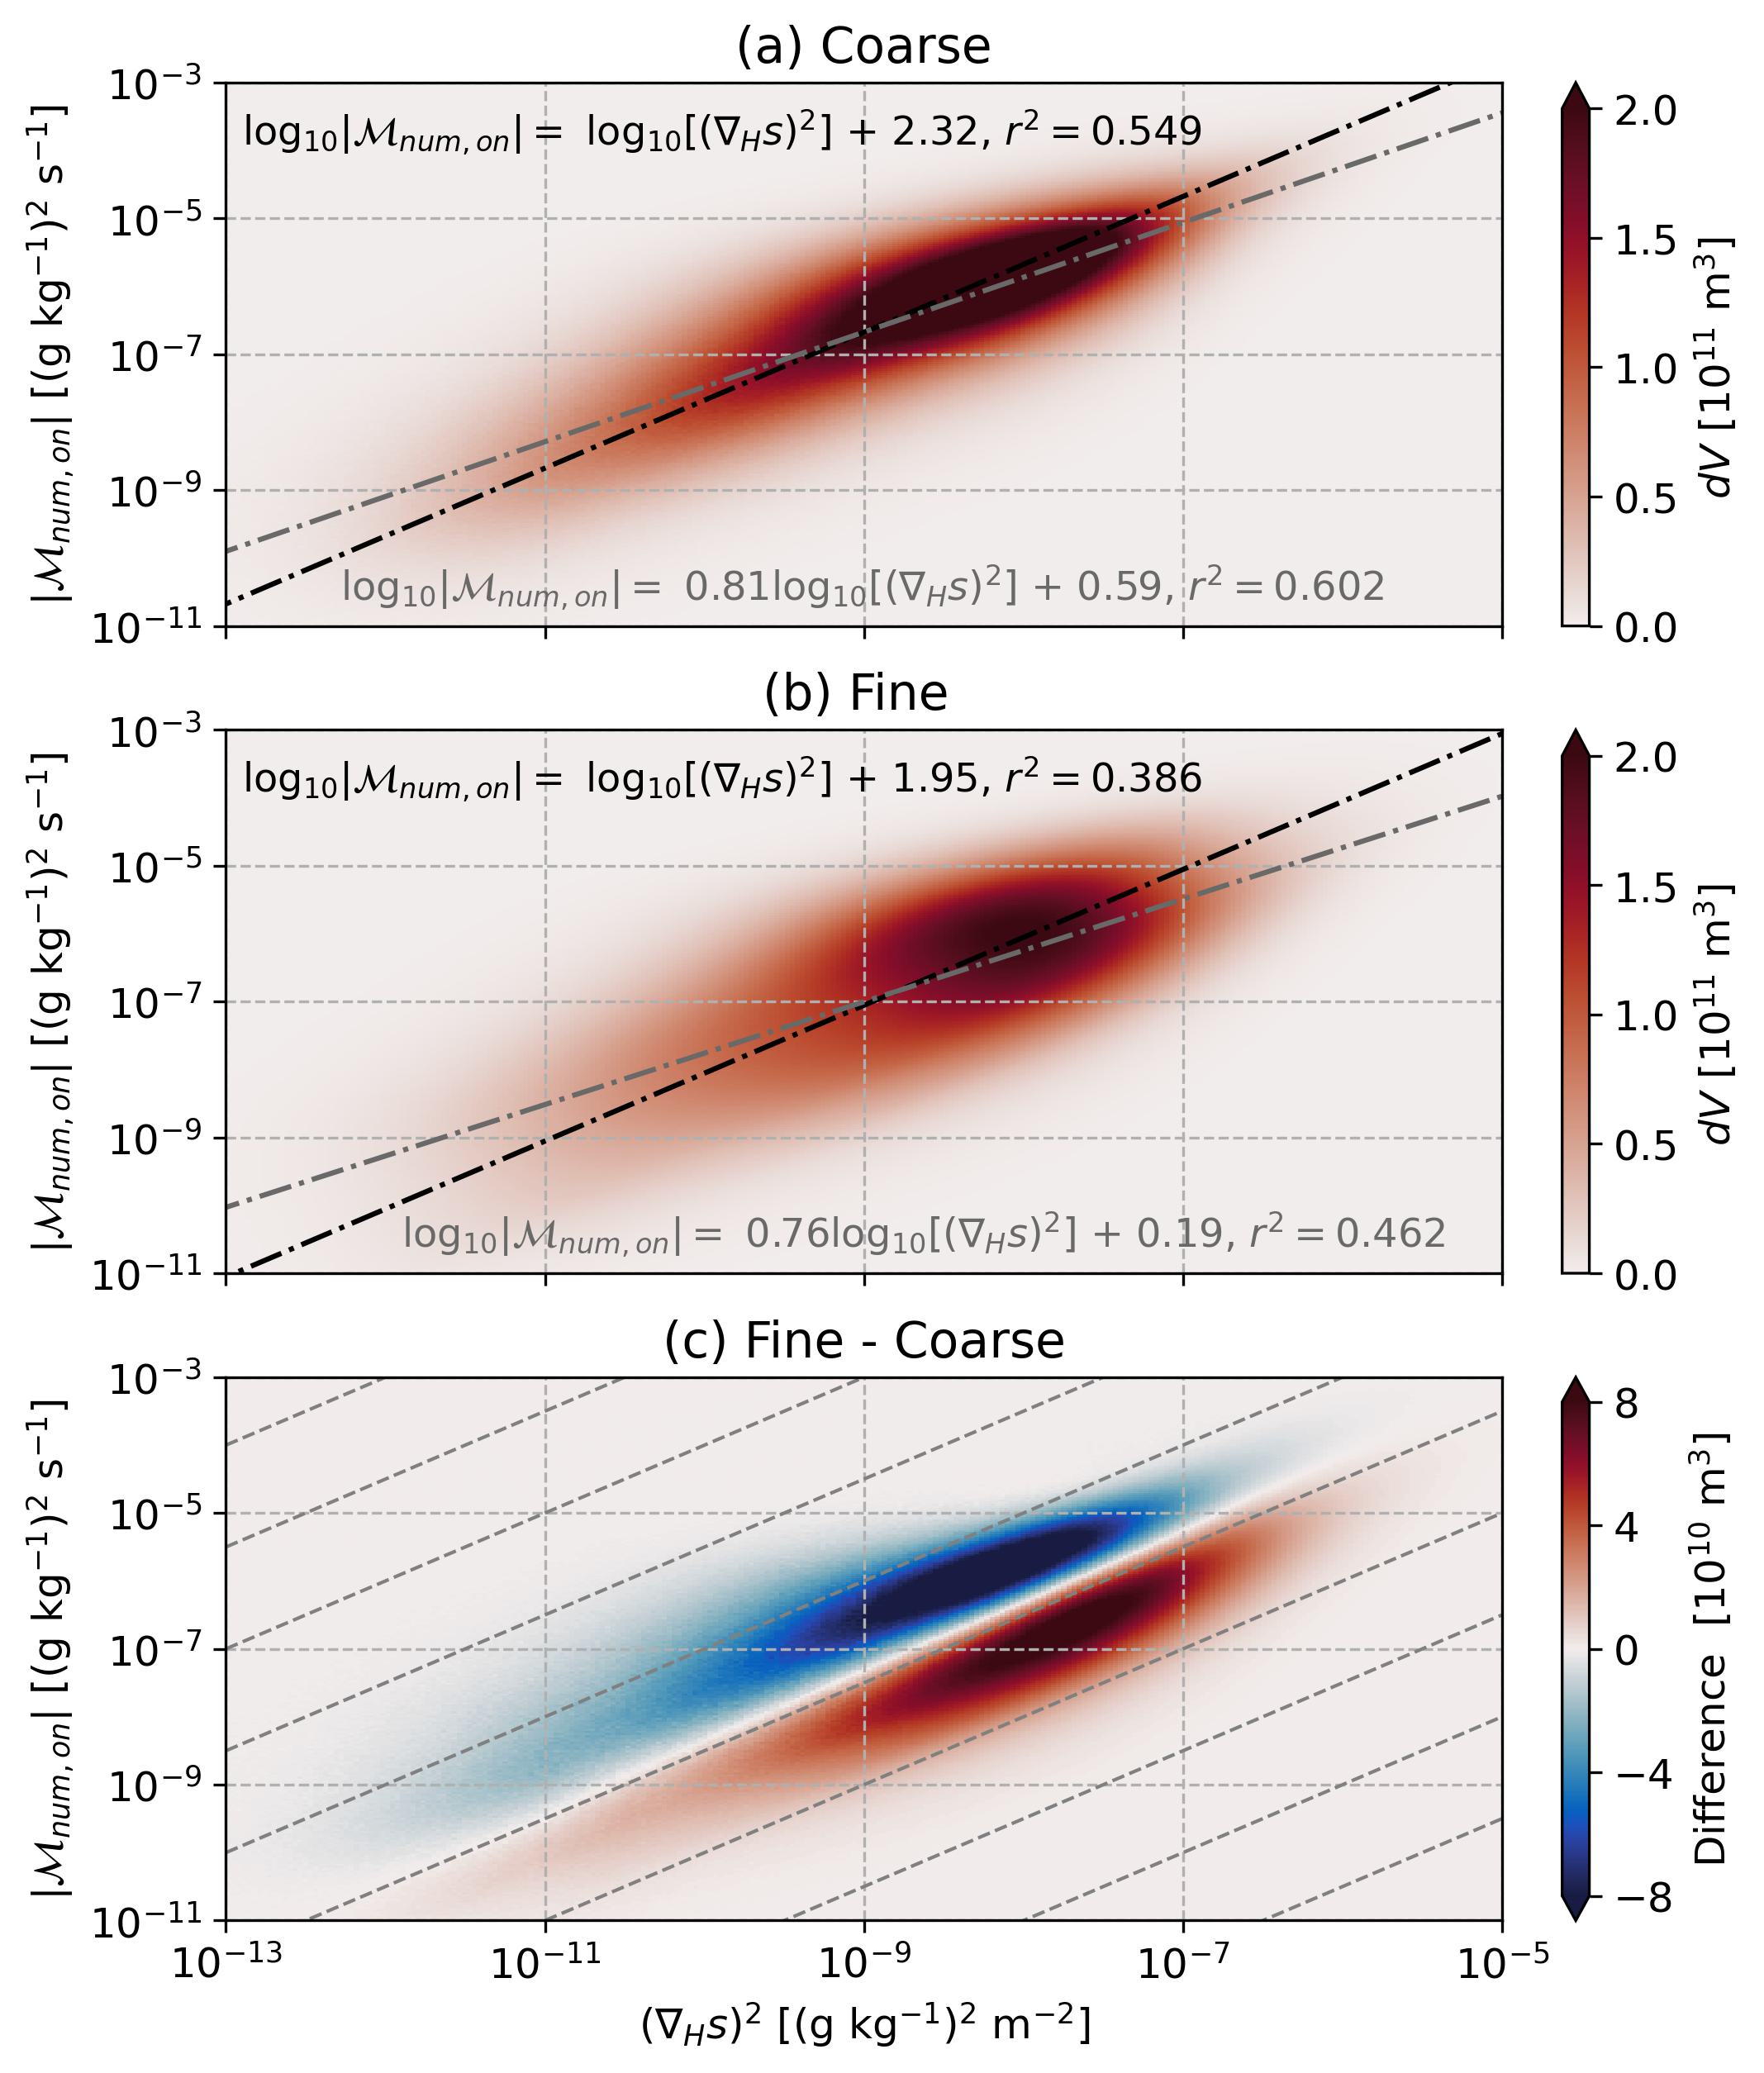
\includegraphics[width =0.9\linewidth]{figures/james_2023/Figure11_sgradmag_histogram.jpg}}
  \caption{Histograms of the horizontal salinity gradient squared $(\nabla_H s)^2$ and absolute value of online numerical mixing $|\mathcal{M}_{num, on}|$ weighted by grid cell volume $dV$ for the coarse (a) and fine (b) simulations, and their differences (c). The thick dashed lines in (a)-(b) display weighted linear regression results for the approximate two-dimensional form of Eq. \ref{eq:mnum_approx} (black) and an empirical fit in log-log space (gray). The regressions and weighted coefficients of determination were obtained by subsampling the coarse grid model every three $\xi,\eta$ points and the fine simulation every 15 points for the entire simulation period. The thick dashed gray lines in (c) indicate a slope of 1.}
  \label{fig:mnum_sgrad}
\end{figure}

As $(\nabla_H s)^2$ increases, more of the domain volume is concentrated at larger values of $\mathcal{M}_{num, on}$. The relationship begins to taper off at $(\nabla_H s)^2 \sim \mathcal{O}(10^{-6})$ g$^2$ kg$^{-2}$ m$^{-2}$, corresponding to salinity gradients associated with surface fronts and the pycnocline in the M/A river plume. These fronts have strong salinity gradients and numerical mixing, but they occupy a small portion of the water column, hence the decrease in grid cell volume. Weaker salinity gradients are associated with longer length and time scales and are correlated with weaker numerical mixing. 

The differences between the coarse and fine simulations demonstrate that the fine simulation has weaker numerical mixing distributed at stronger salinity gradients than the coarse simulation. In other words, for a given salinity gradient, the fine simulation will experience less numerical mixing on average compared to the coarse simulation. The dividing line separating the positive and negative changes to $dV$ between the simulations has a slope of nearly one, suggesting that the change in numerical mixing is proportional to $(\nabla_H s)^2$. The coefficient of determination is lower in the fine simulation because the numerical mixing depends not only on $|\nabla_H s|$, but the components of grid resolution $dV$, water velocities, and the model timestep. In the fine simulation, $\Delta x$ and $\Delta y$ decreased by a factor of five, but the time-averaged volume-integrated numerical mixing decreases by only 35$\%$, suggesting a nonlinear relationship between numerical mixing, the square of the horizontal salinity gradients, and horizontal grid resolution. Although identifying the exact dynamical feedbacks that cause this non-linearity to arise is beyond the scope of this paper, an analysis (not shown) of the instability angle $\phi_{{Ri}_b}$ derived in \citet{Thomas_2013} (their Eq. 8) suggests that the fine simulation is more susceptible to symmetric and inertial instabilities than the coarse simulation. Coupled with the sharp changes of the velocity gradient tensor but insignificant changes to $|\nabla_H s|$ in Figs. \ref{fig:surface_pdfs}-\ref{fig:whole_pdfs}, this is consistent with the idea that different dynamical processes emerge as the resolution is increased, which complicates the relationship between horizontal resolution and numerical mixing. However, had $|\nabla_H s|$ increased significantly, this would have increased the numerical mixing in the fine simulation.

\section{Summary and conclusions} \label{sec:conclusions}

We have studied physical and numerical mixing in a numerical model of the Texas-Louisiana (TXLA) continental shelf using a combination of on- and offline methods based on salinity variance. Physical mixing is defined as the dissipation of salinity variance associated with numerical closure schemes and numerical mixing is defined as the mixing generated by the discretization of salinity advection. Salinity variance can be defined in terms of salinity squared $s^2$ and volume-mean salinity variance $s^{\prime^2}$. Previous research \citep{Burchard_2019, MacCready_2018, Qu_2022_box} has shown the residuals of the $s^2$ and $s^{\prime^2}$ budgets can be used to estimate numerical mixing. However, the robustness of the offline method in realistic simulations has only been assessed qualitatively by \citet{Wang_2021}. The online method, which locally calculates numerical mixing $\mathcal{M}_{num, on}$ as the difference between the advected salinity squared and the square of the advected salinity divided by the model timestep \citep{Burchard_2008}. $\mathcal{M}_{num, on}$ is used to evaluate the accuracy of the offline method. 

We find the residuals of the $s^2$ and $s^{\prime^2}$ budgets, $\mathcal{M}_{num, s^2}$ and $\mathcal{M}_{num, s^{\prime^2}}$, do not converge to the online method. This is true even as the model output frequency is increased to 10 minutes, an impractical output frequency for long-term realistic coastal models at this time. The $s^2$ budget at hourly output may miscalculate numerical mixing by over an order of magnitude. During the study period, $s^2\gg s^{\prime^2}$, which causes the resulting tendency and advection terms in the $s^2$ budget to be over an order of magnitude larger than the $s^{\prime^2}$ budget. We derive the $s^2$ budget in terms of volume-averaged salinity $\overline{s}$ and salinity perturbation $s^\prime$ to relate $\mathcal{M}_{num, s^2}$ and $\mathcal{M}_{num, s^{\prime^2}}$ and investigate the consequences of this scaling. We find the $s^2$ budget experiences larger truncation error compared to the $s^{\prime^2}$ budget when using identical numerical schemes. $\mathcal{M}_{num, s^2}$ begins to converge to $\mathcal{M}_{num, s^{\prime^2}}$ as output frequency increases but is still noisy at 10 minute output. The scaling of $s^2$ and $s^{\prime^2}$ over the shelf is quite different than previous estuarine models \citep{Li_2018, Li_2021, Warner_2020}, where $s^{\prime^2}$ may be similar in scale to $s^2$ since estuary domains include a transition from fresh river water to background coastal salinities. 

The time-averaged $\mathcal{M}_{num, s^{\prime^2}}$ is 60\% larger than the time-averaged $\mathcal{M}_{num, on}$. Although $\mathcal{M}_{num, s^{\prime^2}}$ is much less sensitive to model output frequency, it does not converge to $\mathcal{M}_{num, on}$ for all times and cannot be considered robust. There are many sources of uncertainty that could contaminate the on- and offline methods. For example, a mismatch between our model's in- and external schemes for calculating time derivatives or additional sources of spurious mixing such as grid-scale noise in velocity. 

Consequently, we cannot recommend the offline method for generic quantification of numerical mixing. Although \citet{Wang_2021} qualitatively showed success in estimating numerical mixing offline, we find offline mixing estimates to be inaccurate, and only useful in providing a rough sense and scale of the numerical mixing. Despite this, the offline method qualitatively captures the larger signals in the temporal variability well and might be informative to researchers who are unable to use an online method. We also feel the approach might be useful in comparing different scenarios where the primary questions are about the relative magnitude of numerical mixing. This is particularly relevant for estuarine and coastal models already using a high model output frequency and spatial resolution, but less so for larger-scale models that employ a lower output frequency. 

It is also clear that sources of uncertainty need to be evaluated on a per-model basis, so offline calculation cannot be generally recommended as a primary approach. Given the strong advection and weak physical mixing during summer in the nGoM, we think that our domain is particularly challenging for accurate offline calculation of numerical mixing, and is a good demonstration of the weaknesses of the offline approach. Other regions with relatively stronger physical mixing, e.g., partially mixed estuaries, may be more suitable to the offline approach. However,  a comprehensive understanding of when an offline approach may be feasible is outside the scope of the present study, and so for now we feel the offline approach must be treated as suspect for a particular region until demonstrated otherwise.

Regarding the online analysis, the numerical mixing remains significant relative to the physical mixing even for a submesoscale-resolving coastal ocean model. We find the volume-integrated numerical mixing comprises 57$\%$ of the bulk physical mixing. Instantaneously, the volume-integrated numerical mixing may exceed the physical mixing by almost half an order of magnitude, motivating us to use a two-way nested model with five times the native horizontal grid resolution to examine the sensitivity of numerical mixing to horizontal resolution. We find that the time-averaged volume-integrated numerical mixing decreases by approximately 35$\%$ in the fine simulation, suggesting a nonlinear relationship between horizontal resolution and numerical mixing. Building on the work of \citet{Wang_2021}, we use weighted property histograms to show that numerical mixing is approximately proportional to the square of the horizontal salinity gradients $(\nabla_H s)^2$. As horizontal resolution increases, this relationship weakens because newly resolved dynamical processes emerge, which are evident in histograms of the velocity gradient tensor and $|\nabla_H s|$.  
The salinity field and flow structure for the control volume examined here are dominated by interactions between a rich field of submesoscale eddies, sharp fronts, and strong near-inertial currents. It is encouraging that increasing the horizontal grid resolution decreases the numerical mixing and increases the physical mixing, but at significant computational expense. Another key question resulting from this work is how do changes in numerical and physical mixing at the grid-scale affect the evolution of the mean flow and tracer fields for estuarine and coastal models? We expect numerical mixing to be significant in other realistic simulations of coastal flows, which is particularly relevant for researchers focusing on submesoscale processes, where the impacts of grid-scale numerical mixing are more likely to be pronounced.

\section{Data availability statement} 
All TXLA model output used in this study is publicly available at \url{https://hafen.geos.tamu.edu/thredds/catalog/catalog.html} under the ``TXLA ROMS nested model for SUNRISE/2010" subdirectory. The corresponding analysis code is available at \url{https://doi.org/10.5281/zenodo.7566722}. The calculations were performed in Python ver. 3.9 using the xarray \citep{hoyer_stephan_2021_5771208}, xgcm \citep{abernathey_ryan_p_2022_6643579}, and xroms \citep{xroms} packages. More information about specific packages used for analysis can be found in the code repository. 

% \newpage
% \section{References}
% % % %%% Manually add references after each section
% \bibliographystyle{apalike}
% \begingroup
% \renewcommand{\section}[2]{}%
% \bibliography{references.bib}
% \endgroup % Include the Section2.tex file --- Chapter 1
% !TEX root = ../TAMU_Thesis_Main.tex

%%%%%%%%%%%%%%%%%%%%%%%%%%%%%%%%%%%%%%%%%%%%%%%%%%%%%%%%%%%%%%%%%%%%%%
%%                           SECTION III
%%%%%%%%%%%%%%%%%%%%%%%%%%%%%%%%%%%%%%%%%%%%%%%%%%%%%%%%%%%%%%%%%%%%%

\chapter[footnote={This manuscript is \textit{under review} for the \textit{Journal of Advances in Modeling Earth System}. Reprinted with permission from the American Geophysical Union under the terms of the CC BY license. Full citation:  Schlichting, D., Hetland, R. D., \& Jones, C. S. (2024). Numerical mixing suppresses submesoscale baroclinic instabilities over sloping bathymetry. Authorea Preprints. \url{ https://essopenarchive.org/doi/full/10.22541/essoar.170983234.49281676}}]{Numerical mixing suppresses submesoscale baroclinic instabilities over sloping bathymetry}

\section{Abstract}
In this work, the impacts of spurious numerical salinity mixing ($\mathcal{M}_{num}$) on the larger-scale flow and tracer fields are characterized using idealized simulations. The idealized model is motivated by realistic simulations of the Texas-Louisiana shelf and features oscillatory near-inertial wind forcing. $\mathcal{M}_{num}$ can exceed the physical mixing from the turbulence closure ($\mathcal{M}_{phy}$) in frontal zones and within the mixed layer. This suggests simulated mixing processes in frontal zones may be driven largely by $\mathcal{M}_{num}$. Near-inertial alongshore wind stress amplitude is varied to identify a base case that maximizes the ratio of $\mathcal{M}_{num}$ to $\mathcal{M}_{phy}$. We then we test the sensitivity of the base case with three tracer advection schemes (MPDATA, U3HC4, and HSIMT) and conduct ensemble runs with perturbed bathymetry. Instability growth is evaluated with several analysis methods: volume-integrated eddy kinetic energy ($EKE$) and available potential energy ($APE$), surface and bottom isohaline variability, and alongshore-averaged salinity sections. While all schemes have similar total mixing, HSIMT simulations have over double the volume-integrated $\mathcal{M}_{num}$ and 20\% less $\mathcal{M}_{phy}$ relative to other schemes, which suppresses the release of $APE$ and reduces the $EKE$ by roughly 25\%. HSIMT instabilities are confined shoreward relative to the other schemes. This results in reduced isohaline variability and steeper isopycnals, evidence that enhanced numerical mixing suppresses instability growth.

\section{Plain Language Summary}
Mixing plays a fundamental role in maintaining the general circulation of the ocean by dissipating energy and redistributing tracers, or fluid properties used to track aspects of ocean circulation. Numerical ocean models often parameterize physical mixing processes because their resolution is too coarse to resolve them. Numerical models are also prone to numerical mixing, a type of spurious mixing arising from the discretization of tracer transport by currents. Recent studies have shown numerical mixing can exceed the physical mixing in high resolution models. Here, we study where numerical salinity mixing is significant in the water column and how it impacts the larger-scale circulation and tracer fields in a 500 m resolution, idealized model of the Texas-Louisiana shelf. We find that numerical mixing dominates physical mixing in frontal zones associated with small-scale eddies. To study the impacts of that mixing, we perform an ensemble by varying the numerical scheme for tracer transport. We find that the scheme with excessive numerical mixing suppresses the eddies and prevents the release of their primary energy source. Future studies may use these results as a blueprint to better understand how numerical mixing impacts specific processes near frontal zones and therefore affects model fidelity. 

\section{Introduction} \label{sec:intro}
Mixing, or the irreversible loss of scalar variance by turbulent processes, is a fundamental ocean process because it redistributes tracers and dissipates energy. Recent studies have focused on characterizing numerical mixing -- defined as the spurious mixing generated by the discretization of tracer advection -- because it can be a significant fraction of, or even exceed, the physical mixing. Physical mixing is defined in this study as the destruction of tracer variance prescribed by turbulence closure schemes \citep{Burchard_2008, MacCready_2018}, whereas numerical mixing is generally associated with imperfect discretization of tracer advection. Significant numerical mixing relative to physical mixing has been demonstrated for high resolution estuarine models \citep{Ralston_2017, Rennau_2009, Wang_2021}, submesoscale resolving regional models \citep{Schlichting23}, and a wide range of global models \citep{Griffies_2000, Holmes_2021, Ilicak_2012, megann2018estimating}.

It has been known for decades that spurious mixing can degrade the fidelity of numerical ocean models, driving the model toward unrealistic ocean states. A prominent early example of this was discovered by George Veronis, who showed that the Laplacian diffusion implemented in an ocean circulation model caused unphysical upwelling in western boundary currents \citep{veronis1975role}. The problem resulted from the misalignment of the diffusion tensor and isopycnals, which aliased the prescribed horizontal diffusion as diapycnal diffusion over steeply sloped isopycnals \citep{Griffies_2000} and caused false upwelling near western boundary currents. The ``Veronis effect'' was not mitigated until ocean models employed a rotated diffusion tensor \citep{redi1982oceanic} to minimize spurious diapycnal mixing. Numerical mixing is one source of spurious mixing; there are several others in modern ocean models \cite[see][]{megann2022assessment}. 

While it is often thought of as a source of error in coarse-resolution simulations, numerical mixing can be used in high-resolution simulations as a way to eliminate grid-scale kinetic energy and tracer variance. For example, odd-ordered advection schemes that are numerically dissipative are commonly used in coastal and large eddy simulation (LES) applications \citep{leonard1993positivity, roman2010large, shchepetkin1998quasi,wu2010advection}. In these cases, numerical mixing can be used to improve model stability and fidelity by preventing energy cascading to small scales from gathering at the grid-scale, thereby dominating the solution and creating an unphysical ocean state.

Unlike physical mixing, numerical mixing is not easily controlled by model parameters. This is because numerical mixing is sensitive to many components of the model setup such as the advection scheme \citep{fofonova2021plume,Kalra_2019, Wang_2021}  and grid resolution \citep{Holmes_2021,Ralston_2017,Schlichting23}. It also depends on the resolved flow velocity and tracer gradients \citep{Schlichting23, Holmes_2021, Wang_2021}. Numerical mixing can be negative for advection schemes that attempt to reduce diffusion (e.g., flux-corrected or flux-limited schemes). In this case, tracers may be redistributed up-gradient and spuriously create grid-scale tracer variance. The nonlinear nature of the problem makes it difficult to quantify the larger-scale impacts of numerical mixing without targeted numerical experiments \citep{fofonova2021plume, Kalra_2019}, though it is generally thought that numerical mixing impacts the larger-scale flow and tracer fields differently than the physical mixing in primitive equation models. This is different from implicit LES models, where part of the turbulence cascade is resolved and numerical mixing (in the form of viscous dissipation) reproduces qualitative features of the theoretical and prescribed mixing \citep{domaradzki2003effective, thornber2007implicit}, since the near grid-scale turbulent mixing in these cases is more isotropic. 

It is unclear whether numerical mixing reduces the accuracy of very high resolution primitive equation ocean models capable of permitting or resolving submesoscale processes, since at the resolved scales, the physical mixing is not isotropic. Submesoscales are characterized by $\mathcal{O}(1)$ Rossby and Richardson numbers, a dual cascade of energy, and large vertical motions \citep{McWilliams_2016, taylor2023submesoscale}. Thus, we can expect there to be substantial differences in the character of numerical mixing at these energetic scales, compared to less energetic mesoscales. Submesoscales are important for many oceanographic processes, for example, 1) they restratify the mixed layer and thus play an important role in structuring the ocean's heat budget \citep{boccaletti2007mixed, su2018ocean}, 2) their ageostrophic motions can create a ventilation pathway for bottom trapped material \citep{qu2022rapid} and exchange tracers across the mixed layer base \citep{balwada2021vertical}, and 3) their convergent motions (i.e., fronts) congregate marine organisms and biogenic surfactants \citep{mcwilliams2019survey, ruiz2019effects}. Therefore, it is critical to understand and quantify numerical mixing at sub-kilometer scales as regional coastal models and limited domain open ocean models push towards submesoscale-resolving resolution.

\citet{Schlichting23} quantified volume-integrated numerical and physical mixing of salinity (defined respectively as $\mathcal{M}_{num}$ and $\mathcal{M}_{phy}$ in Section \ref{sec:analysis_tools}) in a submesoscale-resolving simulation of the Texas-Louisiana (TXLA) shelf. They found numerical mixing constitutes about half the total ($\mathcal{M}_{tot} = \mathcal{M}_{num} + \mathcal{M}_{phy}$) mixing and that numerical mixing is correlated with the magnitude of the horizontal salinity gradients $|\nabla_h s| = \left((\partial_x s)^2 + (\partial_y s)^2 \right)^{1/2}$, implying that numerical mixing is significant at fronts associated with submesoscale eddies. These eddies are often found during summer as weakly upcoast winds superimposed with a diurnal land sea breeze cause freshwater from the Mississippi/Atchafalaya river plume to pool over the shelf \citep{Hetland_2017}, which generates strong inertial currents \citep{Kobashi_2020, qu2022rapid}. An example with the two-way nested TXLA model is shown in Fig. \ref{fig:txla_snap} to motivate further analysis.

\begin{figure}
    \begin{center}
    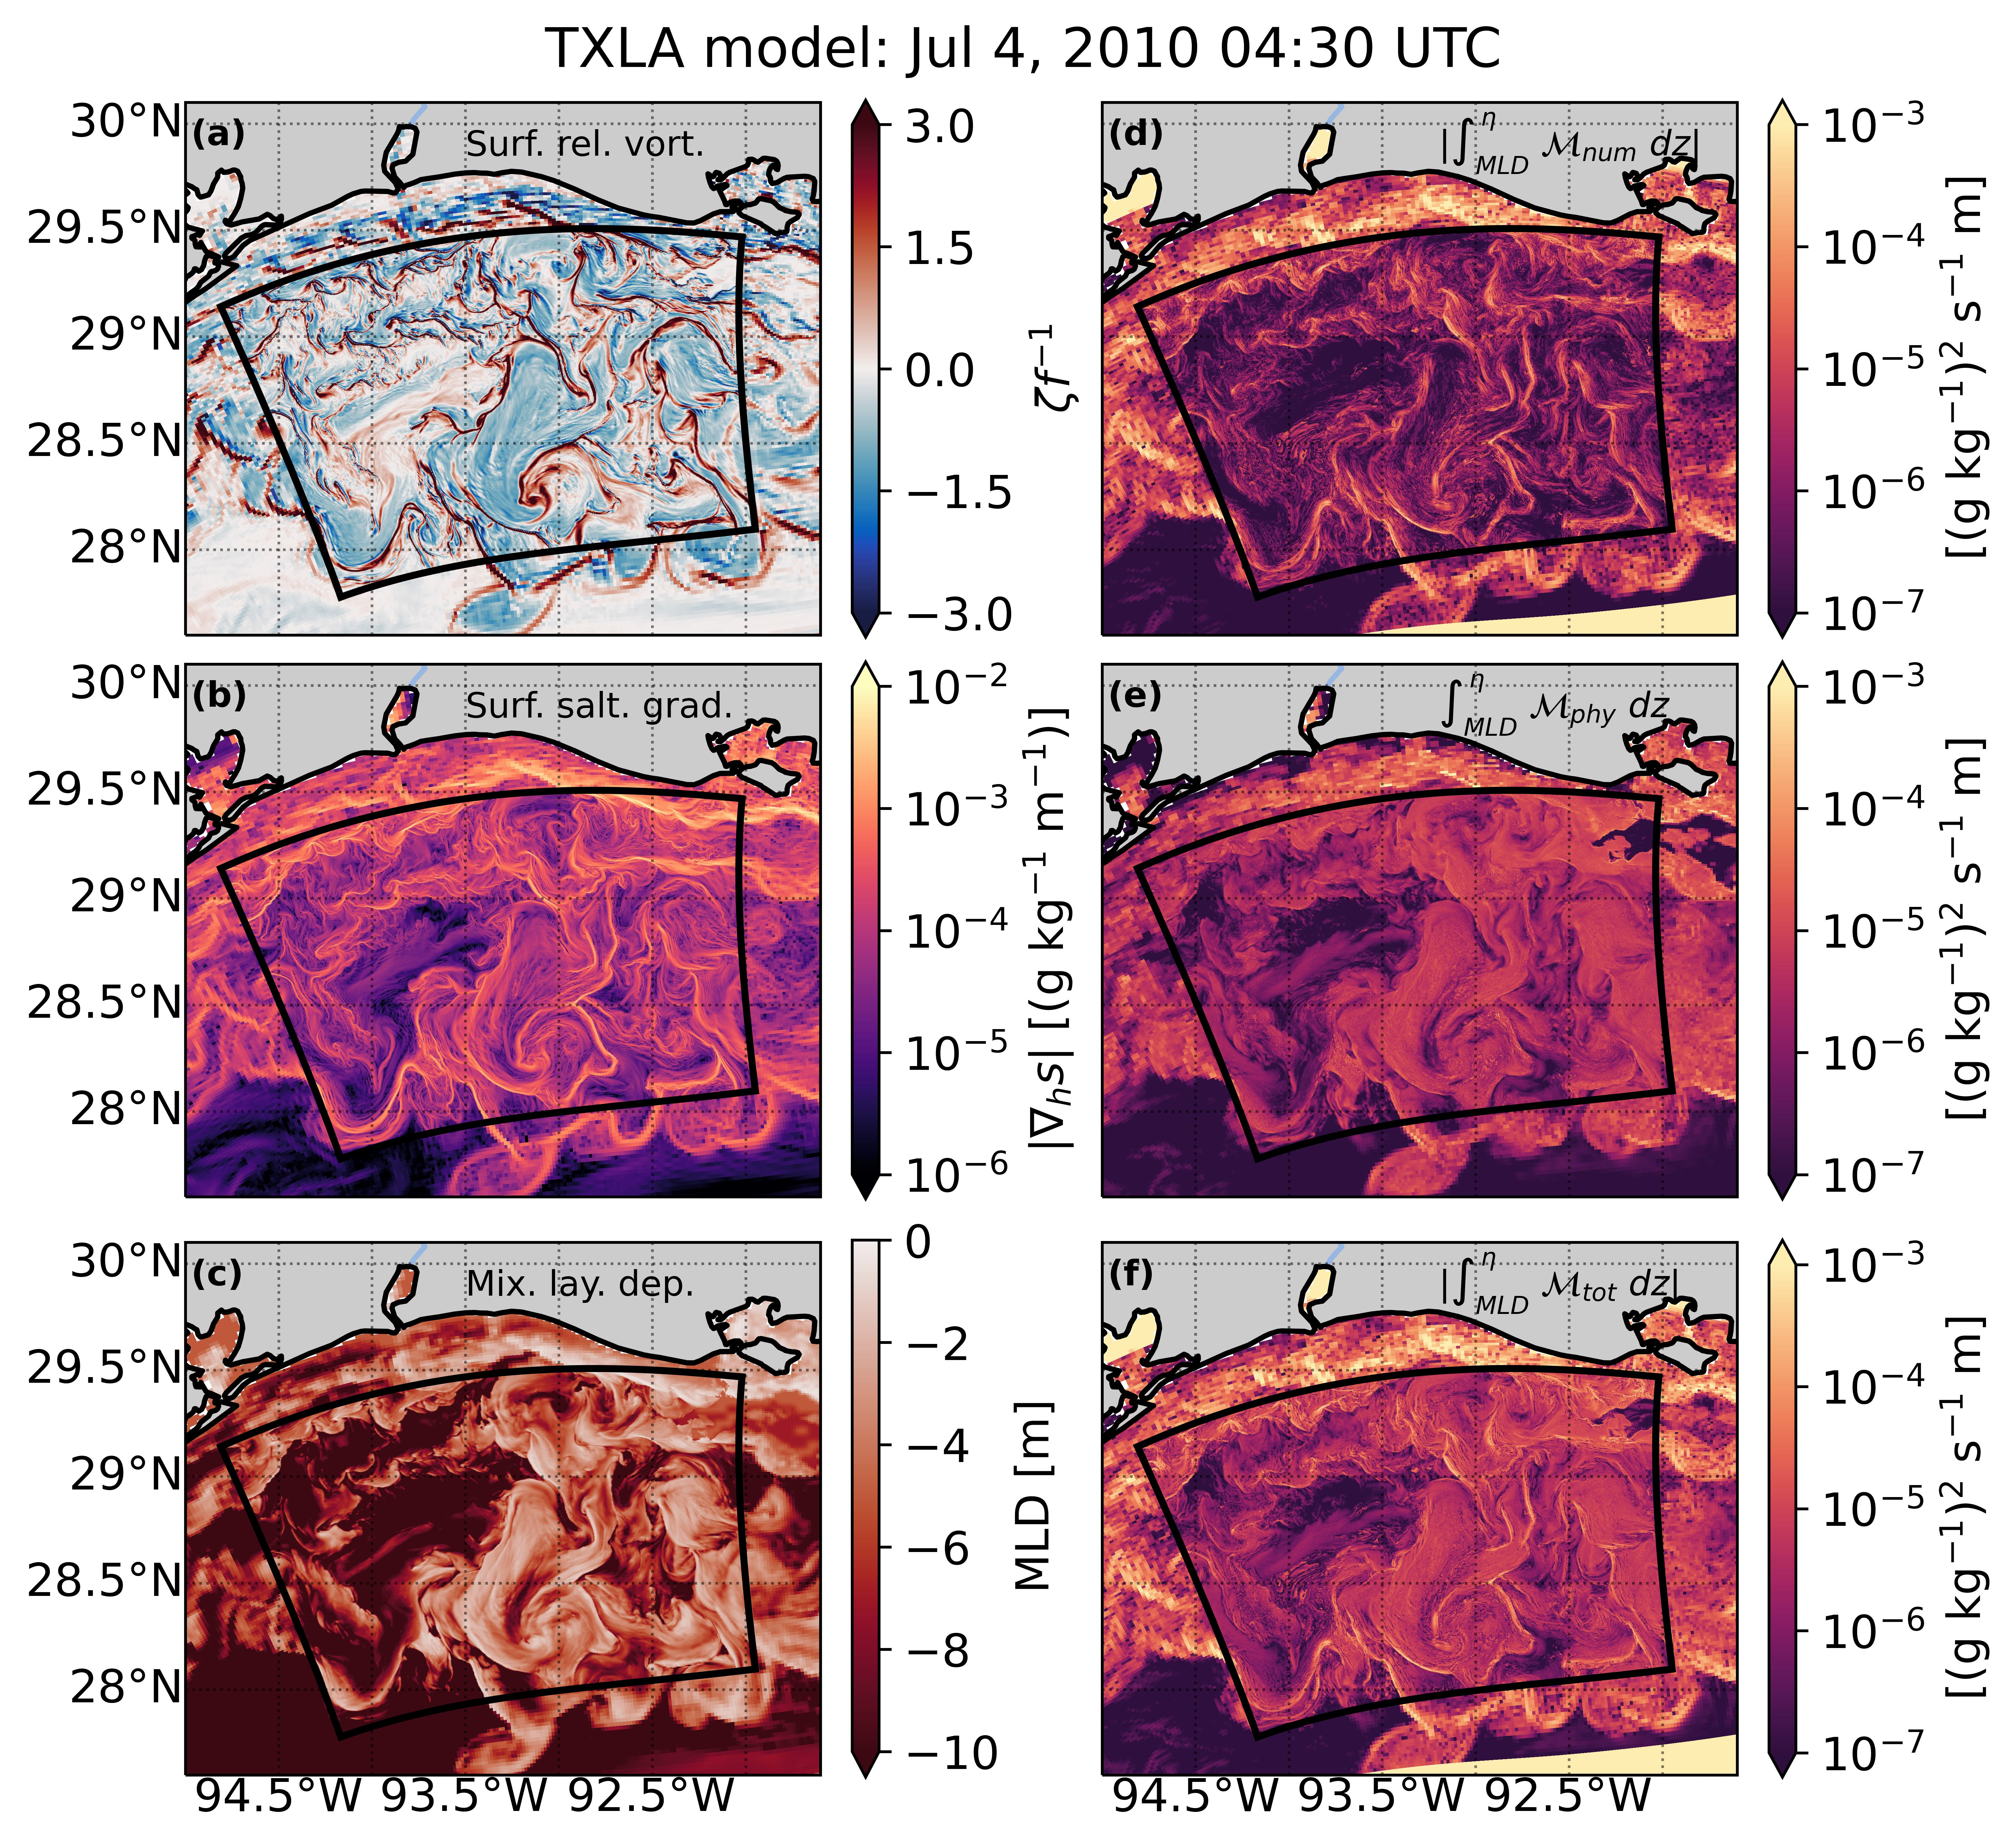
\includegraphics[width = \linewidth]{figures/shelfstrat_2024/txla_snap_int_mld.jpg}\\
    \caption{TXLA model surface $\zeta f^{-1}$ (a), $|\nabla_h s|$ (b), and mixed layer depth (MLD) (c) on July 4, 2010 04:30 UTC. The child domain is marked by the black box. $\mathcal{M}_{num}$ (d), $\mathcal{M}_{phy}$ (e), and $\mathcal{M}_{tot}$ (f) depth-integrated from the base of the mixed layer to the free surface. Note the absolute values are shown in (d) and (f) to account for negative numerical mixing. Here, bulk $\mathcal{M}_{num}/\mathcal{M}_{tot}=24$\% in the child domain. $\mathcal{M}_{num}$ is elevated near the southern boundary of the parent domain and within several bays/estuaries due to coarse grid resolution and close proximity to the open boundary. The colorbars are saturated to emphasize fronts.} \label{fig:txla_snap}
     \end{center} 
\end{figure}

The fronts, marked by normalized relative vorticity $\zeta f^{-1} > 1$, where $\zeta = \partial_x v - \partial_y u$ and $f$ is the Coriolis parameter, are characterized by sharp horizontal salinity gradients. Numerical mixing is depth-integrated from the base of the mixed layer to the free surface and compared with the physical- and total mixing. The mixed layer depth (MLD) is defined using the standard vertical density difference cutoff of 0.03 kg m$^{-3}$ \citep{de2004mixed}. As discussed previously, numerical mixing is significant at fronts due to large horizontal salinity gradients. For the child model domain in Fig. \ref{fig:txla_snap}, numerical mixing constitutes about 24\% of the total mixing. Other definitions of MLD may be used \cite[see][]{thomson2003estimating}, but these do not change the general result that the ratio of numerical- to physical mixing grows as the lower limit of integration shoals. For example, depth-integrating over the top one m of the water column to the free surface increases this ratio to 52\%. When the eddies are less perturbed by regional forcing \citep[e.g., Fig. 2 of][]{Schlichting23}, this ratio can exceed 75\%. This implies that even as the horizontal resolution is pushed towards submesoscale resolving, mixing processes in the frontal zone may be numerically driven. More broadly, this reinforces the idea that numerical mixing can dominate in regions where physical mixing is weak \citep{Kalra_2019, Wang_2021}.

The primary goal of this paper is to characterize and quantify the numerical mixing in a submesoscale eddy-resolving model, and to gain insight into how this numerical mixing impacts the larger-scale ocean state. It is difficult to address this with a realistic model due in part to the large computational cost, but also the difficulty in quantifying the difference in model states with different numerical mixing in a complex, realistic model. We therefore use an idealized model based on \citet{Hetland_2017} that captures many of the characteristics of the submesoscale eddy field seen in the realistic model. We use three different advection schemes as a way to modify the numerical mixing across different simulations. We then assess the impact of these different advection schemes through alongshore means in the idealized model -- an analysis that is not possible in the realistic model. Our primary finding is that numerical mixing suppresses the release of available potential energy, impacting the eddy field and the offshore extent of the fresh water front.


\section{Numerical models} \label{sec:model_setup}
Both models are implementations of the Regional Ocean Modeling System \citep[ROMS,][]{shchepetkin2005regional} configured as part of the Coupled-Ocean-Atmosphere-Waves-Sediment-Transport model \citep[COAWST, ver. 3.7,][]{Warner_2010}.

\subsection{Realistic ROMS model}
The two-way nested TXLA model setup is described in \citet{Schlichting23}. The sub-domain marked with a black box in Fig.~\ref{fig:txla_snap} is the higher-resolution child model (which is nested in a coarser resolution parent model): in this paper we exclusively use the child model. Only details necessary to compare with the idealized model are provided. The horizontal resolution of the child model spans from approximately 255 m close to the coast to 357 m near the offshore boundary with a mean resolution of 315 m. The model uses 30 vertical layers with functions (vtransform=2, vstretching=4) and stretching parameters ($\theta_s = 5,\theta_b=0.4$). The vertical resolution in the top m of the water column ranges from 13 cm close to the coast to 73 cm near the southern boundary, with a mean resolution of 38 cm. 
The lowest vertical resolution is about 36 m over the continental slope. As discussed above, this model exhibits significant numerical mixing near the ocean surface. To elucidate the causes and effects of this numerical mixing, we created an idealized model in a similar regime to the realistic model. 
 
\subsection{Idealized ROMS model}
The model configuration follows \citet{Hetland_2017} and is based on a water mass analysis of summer conditions over the TXLA shelf (see his Fig. 5). ROMS is configured as a reentrant shelf with periodic alongshore boundary conditions and a wall at the coast (Fig. \ref{fig:ideal_ics}). The domain is 97 km in the along- and across-shore directions with a horizontal resolution of 500 m. The vertical grid parameters are the same as the realistic model. The minimum water depth is five m at the coast and approximately 103 m at the offshore boundary with a bottom slope of 0.001. Over the initially stratified region, the vertical resolution is about 16 cm in the top one m of the water column and one m over the entire water column, with the coarsest vertical resolution being 6.8 m close to the bottom. A small amount of random noise equal to 1\% of the local depth is added to the bathymetry to force instabilities. The offshore boundary conditions for the free surface and depth-averaged currents use a Chapman-Flather combination \citep{chapman1985numerical,flather1976tidal}. The three-dimensional variables use a no gradient condition at the offshore boundary. While a no-gradient boundary condition is unrealistic, we analyze the near-inertial wind ensemble runs described in Section \ref{sec:results} before eddies interact with the offshore boundary. 

\begin{figure}[t]
    \begin{center}
    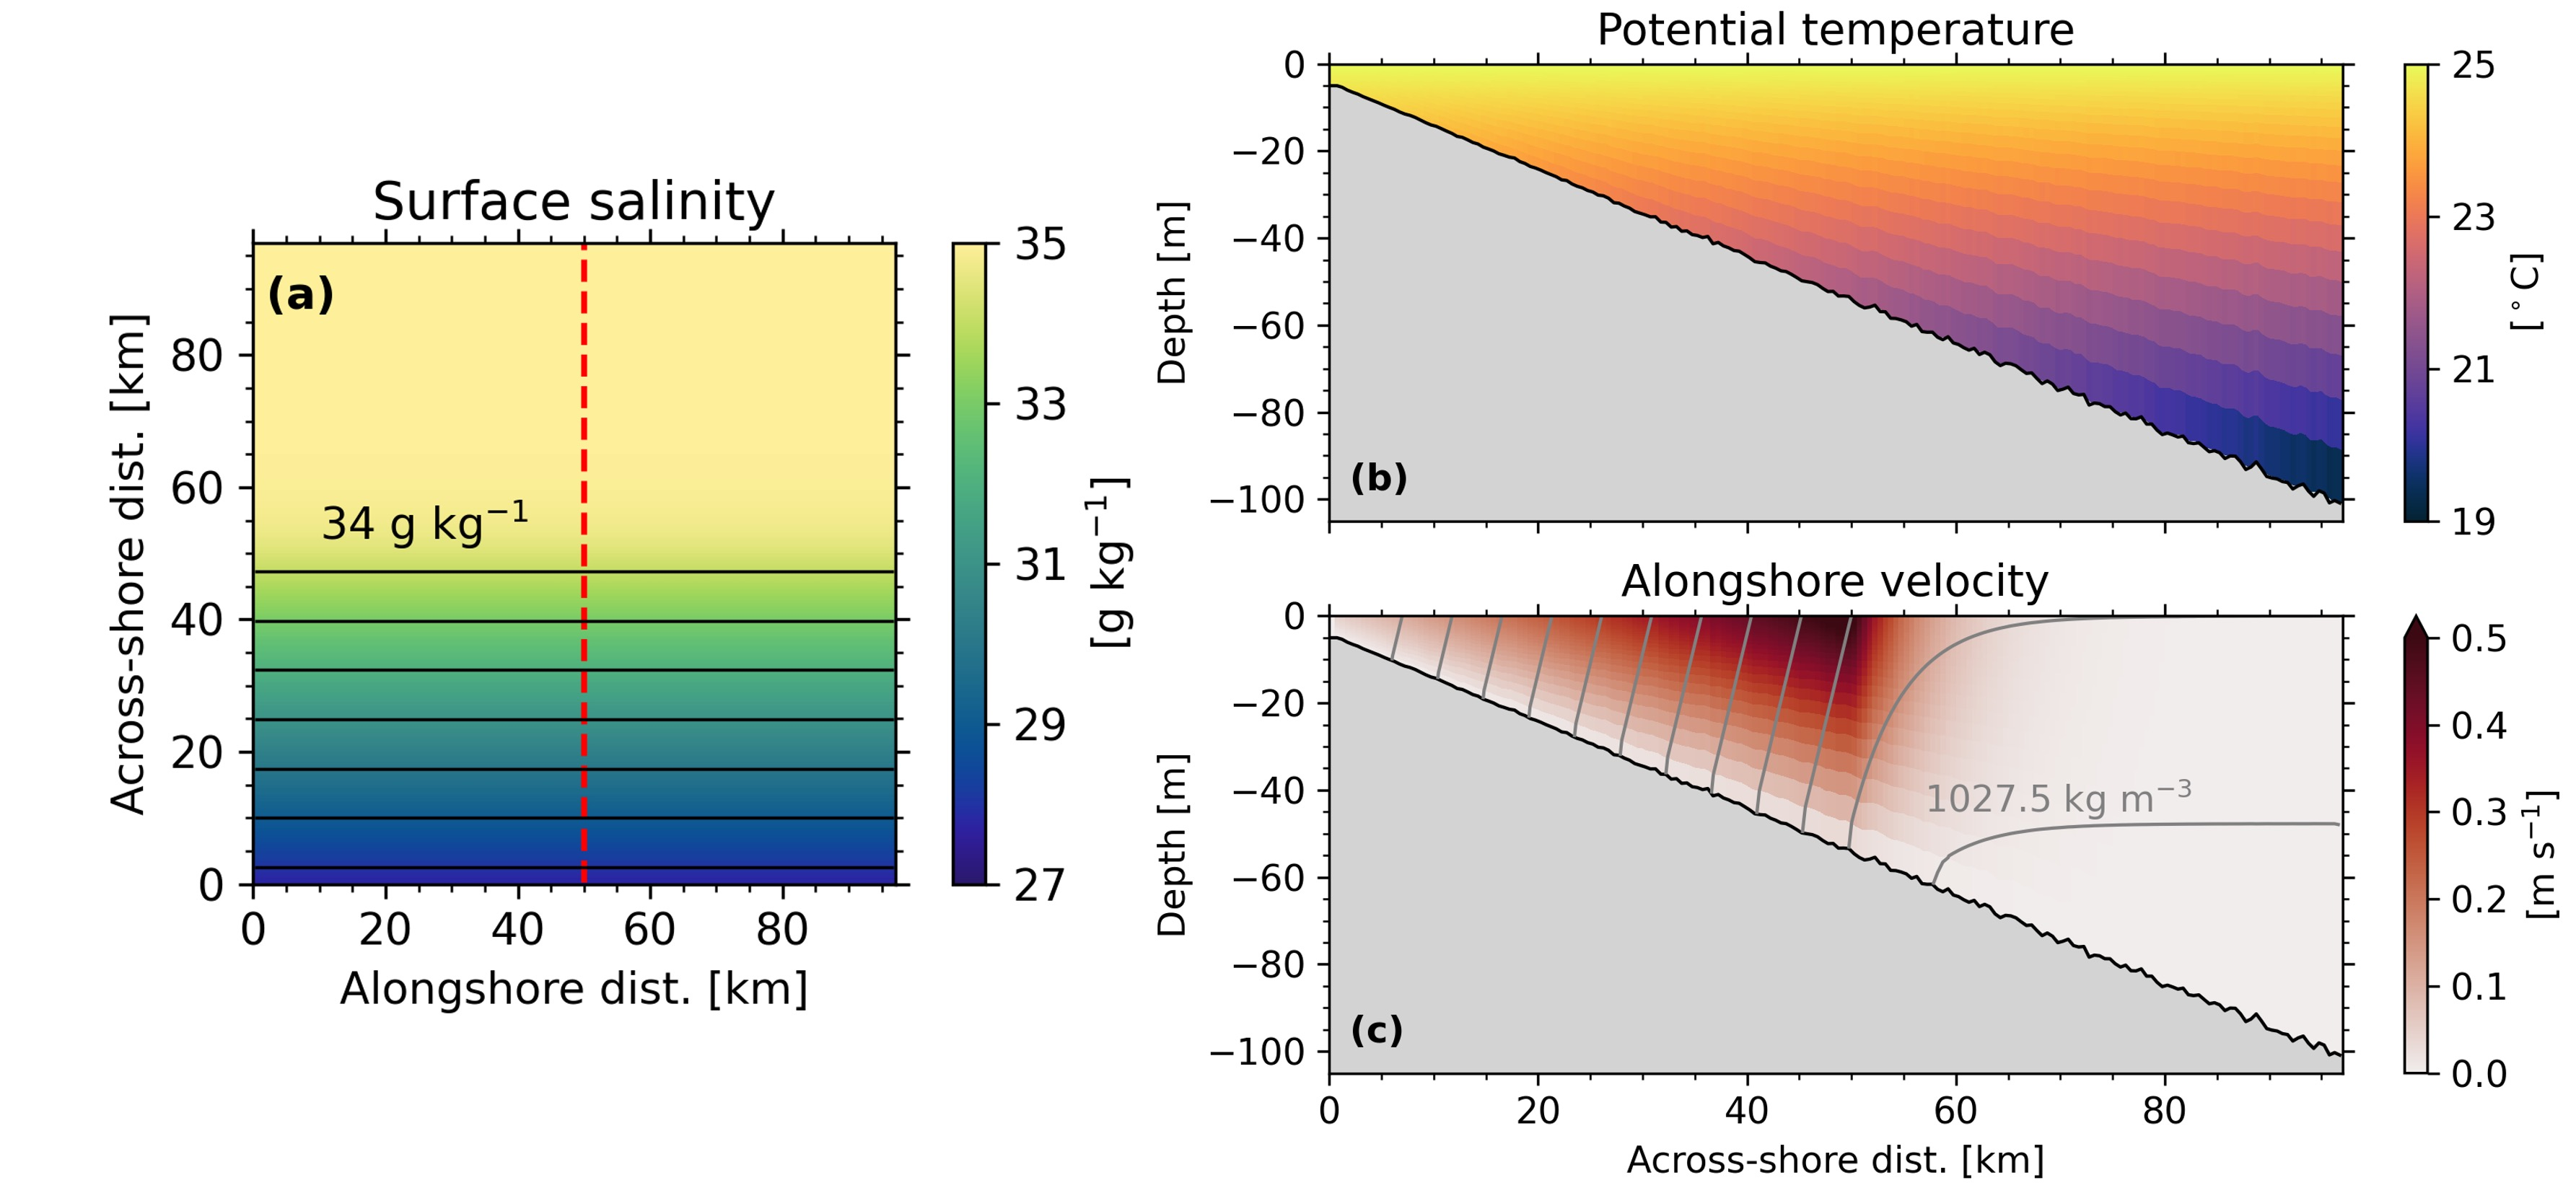
\includegraphics[width = \linewidth]{figures/shelfstrat_2024/initial_conditions_1.jpg} \\
    \caption{Idealized model initial conditions. Plan view of surface salinity (a) with isohalines overlaid every g kg$^{-1}$ and cross-sections of potential temperature (b) and alongshore velocity (c) with isopycnals overlayed every 0.5 kg m$^{-3}$. The cross-sections are shown at the red dashed line in (a).} \label{fig:ideal_ics}
     \end{center}
\end{figure}

The model is run on an $f$ plane with the Coriolis parameter $f$ set to $10^{-4}$ s$^{-1}$ ($\sim$ 43.5$^\circ$N) such that the inertial period is about 17.4 hours. Multidimensional Positive Definite Advection (MPDATA) is used for tracer advection \citep{Smolarkiewicz_1998} for all runs until specified otherwise. The $k-\epsilon$ turbulence closure scheme is used to parameterize the vertical mixing \citep{umlauf2003generic, Warner_2005}. No explicit lateral mixing scheme is prescribed. The model initial conditions (Fig. \ref{fig:ideal_ics}) are specified in terms of two non-dimensional parameters: the Richardson Number ($Ri=N^2f^2M^{-4}$) and slope Burger number $S=Nf^{-1}\alpha$. $N$ is the buoyancy frequency, $M^2$ is the magnitude of the lateral buoyancy gradients $|\left(\nabla_h b \right)^2|$, and $\alpha$ is the bottom slope. The resulting values of Ri and S are 1.0 and 0.1, respectively. The initial salinity varies only in the horizontal with a constant across-shore gradient inshore of 50 m depth with $M^2=10^{-6}$s$^{-2}$. The initial temperature field varies only in the vertical with $N^2 = 10^{-4}$s$^{-2}$. Density $\rho$ uses a linear equation of state:
\begin{equation} \label{eqn:EOS}
    \rho = 1027 \left[1+7.6 \times 10^{-4}(s-35)-1.7 \times 10^{-4} (\theta-25) \right] \, , 
\end{equation}
where $s$ is the salinity and $\theta$ is the temperature.
The alongshore flow is initialized with geostrophic vertical shear and no flow at the bottom. The bottom boundary layer uses a logarithmic velocity profile with a bottom roughness of 0.003 m.

\section{Analysis methods} \label{sec:analysis_tools}

\subsection{Energetics}
Volume-integrated energetics are used to explore how baroclinic instability affects the stratification and eddy kinetic energy. A Reynolds decomposition $\mathbf{u}=\overline{\mathbf{u}}+\mathbf{u}^\prime$ is used to divide the flow into a mean $\overline{\mathbf{u}}$ and fluctuating $\mathbf{u}^\prime$ component, with $\mathbf{u}$ denoting the horizontal velocity vector. Due to the periodic boundary condition, we follow \citet{Hetland_2017} and define $\overline{\mathbf{u}}$ with an alongshore mean:
\begin{equation}
    \overline{\mathbf{u}}=\frac{1}{L} \int_0^L \mathbf{u} \, dx
\end{equation}
such that $\mathbf{u}^\prime$ is the perturbation from the alongshore mean. The total kinetic energy ($TKE$), mean kinetic energy ($MKE$), and eddy kinetic energy ($EKE$) are defined as \citep{cushman2011introduction}:
\begin{equation} \label{eqn:tke}
    TKE = \frac{1}{2}(u^2+v^2) ,
\end{equation}
\begin{equation} \label{eqn:mke}
    MKE = \frac{1}{2}(\overline{u}^2+\overline{v}^2) ,
\end{equation}
\begin{equation} \label{eqn:eke}
    EKE = \frac{1}{2}(u^{\prime^2}+v^{\prime^2}) .
\end{equation}
Note that \citet{Hetland_2017} defined $MKE$ as a function of $\overline{u}$ only and thus $EKE$ was calculated as $\frac{1}{2}(u^{\prime^2}+v^{2})$. This is because the alongshore mean of the across-shore velocity $\overline{v}$ is initially zero and negligible without wind forcing. However, this is not the case when oscillatory alongshore wind forcing is added, so we calculate $v^\prime$ with reference to an alongshore mean. Volume-integrated versions of Eqs. \ref{eqn:tke}-\ref{eqn:eke} over the initially stratified region will be used to determine when to analyze mixing and to get an understanding of how wind forcing affects instability development. They are normalized by the initial $MKE$ ($MKE_0$) so the initial $TKE$ and $MKE$ are one. Thus, 
\begin{equation}
    TKE_n = \frac{\iiint TKE \, dV}{\iiint MKE_0 \, dV},
\end{equation}
\begin{equation}
    MKE_n = \frac{\iiint M
    KE \, dV}{\iiint MKE_0 \, dV},
\end{equation}
\begin{equation}
    EKE_n = \frac{\iiint EKE \, dV}{\iiint MKE_0 \, dV}.
\end{equation}

\subsection{Volume-averaged salinity variance}
\citet{Li_2018} showed that salinity variance can be used to characterize the stratification within a control volume. The salinity variance is also defined using a Reynolds decomposition. We split the salinity into a volume-averaged ($\overline{s}$) and fluctuating ($s_{tot}^\prime$) component such that the total variance is written as  
\begin{equation}
        s_{tot}^{\prime^2} = (s-\overline{s})^2, \, \, \xrightarrow{} \overline{s} = \frac{1}{V} \iiint s \, dV.  
\end{equation}

This can be decomposed into vertical ($s_v^{\prime^2}$) and horizontal ($s_h^{\prime^2}$) components. For example, $s_v^{\prime^2} = (s-\Tilde{s})^2$ is defined with the vertically-averaged salinity $\Tilde{s}$. After some manipulation, it follows that the volume-averaged total salinity variance can be decomposed as:
\begin{equation} \label{eqn:vavg_svar}
        \frac{1}{V} \iiint s_{tot}^{\prime^2} \, dV = \frac{1}{V} \iiint s_{h}^{\prime^2} \, dV + \frac{1}{V} \iiint s_{v}^{\prime^2} dV. 
\end{equation}
Eq. \ref{eqn:vavg_svar} is the volume-averaged version of Eq. 8 from \citet{Li_2018}. $s_h^{\prime^2}$ can be calculated by quantifying $s_{tot}^{\prime^2}$ and $s_{v}^{\prime^2}$ individually and subtracting the two. Previous studies have reported estimates of $\iiint s_{tot}^{\prime^2} \, dV$ \citep{Wang_2018, Burchard_2019}. However, this can be difficult to physically interpret because it scales with $V$. Volume-averaging alleviates this and allows for direct comparison with other estuaries and coastal regions.  

\subsection{Quantification of mixing}
Physical mixing is defined as the dissipation of salinity variance \citep{Burchard_2008, MacCready_2018}:
\begin{equation}
        \mathcal{M}_{phy} = 2 \kappa_v \left(\partial_z s \right)^2, 
\end{equation}
where $\kappa_v$ is the vertical salinity diffusivity. 

Numerical salinity mixing is calculated following \cite{Burchard_2008}:
\begin{equation} \label{eq:mnum}
        \mathcal{M}_{num} = \frac{A\{ s^2 \}-\left(A \{s \} \right)^2}{\Delta t} \quad ,
\end{equation}
where $A$ is the advection operator (i.e., MPDATA) and $\Delta t$ is the online timestep. While \citet{Klingbeil_2014} improves the \citet{Burchard_2008} algorithm, it is not coded into the ROMS source code. $\mathcal{M}_{num}$ and $\mathcal{M}_{phy}$ are calculated online so errors associated with offline analysis do not contaminate the calculations \citep{Schlichting23}.

\subsection{2D Frontogenesis function}
Future studies may benefit from understanding how $\mathcal{M}_{num}$ changes as horizontal tracer gradients are sharpened by frontogenesis and weakened by frontoloysis. One way to conceptualize this is with the frontogenesis function $FGF$ \citep{hoskins1982mathematical, mcwilliams2021oceanic}. In two-dimensions, this describes whether advective processes are sharpening ($FGF>0$) or weakening ($FGF<0$) horizontal buoyancy gradients. $FGF$ is defined as the dot product of the tracer gradients with their Lagrangian rate of change. While typically expressed in terms of lateral buoyancy gradients, we write $FGF$ in terms of salinity because surface stratification is provided only by salinity:
\begin{equation} \label{eqn:fgf_2d}
        FGF = \frac{1}{2}\frac{D}{Dt} \left(\nabla_h s \right)^2,
\end{equation}
where $\frac{D}{Dt} = \partial_t(.) + \mathbf{u}_h \cdot \nabla_h (.)$ is the material derivative excluding the vertical term. 

Eq. \ref{eqn:fgf_2d} can be normalized so that it may compared directly with other dynamical properties. For example, \citet{barkan2019role} showed that divergence $\delta  = (\partial_x u + \partial_y v)$ is a dominant parameter driving submesoscale frontogenesis. $FGF$ can be normalized by $f$ such that it may be compared to a rotational timescale. $FGF$ can be further normalized by $\nabla_h s$, which we define as the normalized frontogenesis function $nFGF$:
\begin{equation} \label{eqn:fgf_norm}
    nFGF = \frac{1}{2f \left(\nabla_h s \right)^2}\frac{D}{Dt} \left(\nabla_h s \right)^2,
\end{equation}
which is $\mathcal{O}(1)$ when submesoscale frontogenesis and frontolysis occurs. Thus, Eq. \ref{eqn:fgf_norm} describes the time rate of change of the distance between two isohalines relative to the Coriolis parameter. In other words, the normalized rate of cross-frontal convergence and divergence. For example, $nFGF=1$ indicates horizontal salinity gradients will collapse over one rotational timescale. $nFGF = -1$ indicates a front will expand over a rotational timescale. 

\section{Results} \label{sec:results}
\subsection{Unforced- and base case}
We start with a brief description of the near-inertial wind ensemble then compare the temporal evolution of the instabilities between the unforced- and base case. An overview of how wind forcing affects properties related to mixing in other ensemble members are provided in the appendix because they are not directly related to the primary objective of this study. A total of 15 ensemble members, each with different wind forcing, were run for 20 days (Fig. \ref{fig:wind_ensembles}). Each member is named according to the amplitude of the near-inertial (0.92$f$) alongshore wind stress $\tau_0^x$. The spatially-uniform wind stress $\tau^x$ is calculated as
\begin{equation}
    \tau^x = \tau_0^x \sin(0.92 f t) \, , 
\end{equation}
where $t$ is time. The first three days are set to zero so wind forcing starts as the instabilities begin forming (Fig. \ref{fig:time_series_base}). The wind stress is prescribed to mimic the near-resonance between the diurnal winds over the TXLA shelf and the regional inertial frequency \citep{Qu_2022_NIW}. The same bathymetry is used in all ensemble members.

\begin{figure}[t!]
    \begin{center}
    \includegraphics[width = 0.9\linewidth]{figures/shelfstrat_2024/time_series_shelf_overview_vavg.jpg}\\
    \caption{Comparison between the base- and unforced case. (a) Alongshore wind stress $\tau_x$ prescribed at each surface grid cell. (b) Normalized, volume-integrated energetics as defined in text. (c) Volume-averaged $\mathcal{M}_{num}$ and $\mathcal{M}_{phy}$. The absolute value is taken to account for negative volume-integrated $\mathcal{M}_{num}$ before the instabilities form. As in (c), but depth-integrated from the base of the mixed layer to the free surface (d) and from the top one m to the free surface (e). (f) Volume-averaged salinity variance decomposition as defined in Eq. \ref{eqn:vavg_svar}. The shaded areas indicate time used for computation of bulk values.}\label{fig:time_series_base}
     \end{center}
\end{figure} 

The base case (0.1 Pa ensemble member, Fig. \ref{fig:time_series_base}) was identified as the ensemble member with the maximum ratio of volume-integrated $\mathcal{M}_{num}$ to $\mathcal{M}_{phy}$ (Fig. \ref{fig:wind_ensembles} d). The base case features a $\tau_x$ amplitude that is slightly more energetic than the magnitude of the diurnal wind stress amplitude in the realistic simulation. However, as we show later (Fig. \ref{fig:jpdf}), the representation of frontogenesis and frontolysis is statistically similar to the realistic model. By selecting the ensemble member with maximum $\mathcal{M}_{num}$ to $\mathcal{M}_{phy}$, we assume it is easier to identify the larger-scale impacts of $\mathcal{M}_{num}$ on the solution with the tracer advection experiments. All quantities hereafter are analyzed inshore of the initially stratified region, indicated by the black contours in Fig. \ref{fig:ideal_ics} (a). 

Normalized volume-integrated energetics for the case with no wind forcing are shown by dashed-dotted lines in Fig. \ref{fig:time_series_base} (b). As indicated by $EKE_n$ and consistent with \citet{Hetland_2017}, the eddy field in the unforced case forms as an organized disturbance after day three. By day ten, the instabilities are mature and never interact with offshore boundary. The $TKE$ and $MKE$ decrease as the instabilities develop due to the bottom friction, which provides a forward cascade of energy via dissipation in the bottom boundary layer. 

Volume-averaged $\mathcal{M}_{phy}$ and $\mathcal{M}_{num}$ are shown for three depth ranges: 1) The entire water column (Fig. \ref{fig:time_series_base} c), 2) from the base of the mixed layer to the free surface (Fig. \ref{fig:time_series_base} d), and the top one m to the free surface (Fig. \ref{fig:time_series_base} e). All quantities are volume-averaged so changes to $V$ for the different depth ranges are taken into account. For all depth ranges, both mixing quantities increase as the instabilities form, but exhibit different temporal variability. However, bulk values are computed with volume-integrals because we are interested in the integrated effects that changing the wind forcing has on mixing. From days 7.5-15, the ratio of bulk $\mathcal{M}_{num}$ to $\mathcal{M}_{phy}$ is 6.5\%. For the entire water column, $\mathcal{M}_{phy}$ increases until the instabilities are mature then reaches near steady-state as they penetrate further into the water column and relax the mean flow. $\mathcal{M}_{num}$ maximizes near day seven then decreases for the remainder of the simulation as $|\nabla_h s|$ weakens.

Volume-averaging from the base of the mixed layer increases the ratio of bulk $\mathcal{M}_{num}$ to $\mathcal{M}_{phy}$ to 24.9\%, indicating that numerical mixing becomes more important in the mixed layer. From days 8-11, $\mathcal{M}_{num}$ declines by over an order of magnitude before returning to previous levels. This variability is not seen in time series of $\mathcal{M}_{num}$ for the ensemble members with wind forcing, which all reach a near periodic state in days 8-11. Identifying the exact cause of this decrease is beyond the scope of this paper. $\mathcal{M}_{phy}$ reaches steady state on day ten as with the entire water column. Over the top one m of the water column, $\mathcal{M}_{num}$ rapidly increases as the eddies develop and is comparable to $\mathcal{M}_{phy}$ for froms Days 7.5-15, then gradually declines as the fronts are dissipated by bottom friction. The ratio of bulk $\mathcal{M}_{num}$ to $\mathcal{M}_{phy}$ increases to 104.8\%. These results validate the arguments suggested in Section \ref{sec:intro}; that is, even in a 500 m resolution idealized model, mixing processes near the frontal zone may be driven by $\mathcal{M}_{num}$. 

Energetics and mixing rates are related to the volume-averaged salinity variance. Until day four, $s_{tot}^{\prime^2}$ consists only of $s_{h}^{\prime^2}$ due to the initial conditions, as shown in Fig. \ref{fig:time_series_base} (f).  $s_{tot}^{\prime^2}$ slightly increases until the instabilities mature on day ten as the isopycnal slope is reduced.  $s_{h}^{\prime^2}$ is gradually converted to $s_{v}^{\prime^2}$ via differential advection of horizontal salinity gradients \citep{Li_2018} and restratification by mixed layer instabilities \citep{boccaletti2007mixed}. As the eddies are dissipated by bottom friction, the water column is mixed horizontally such that $s_{h}^{\prime^2}$ decreases. In the estuarine community, this process is referred to as tidal straining \citep{simpson1990tidal}. The key difference in our model is this process is forced by submesoscale baroclinic instabilities -- not tidal forcing. $s_{tot}^{\prime^2}$ is $\mathcal{O}(3 \text{(g kg}{^{-1}})^{2})$, less than half that of the TXLA child model domain (Fig. 7 of \citet{Schlichting23}) and about an order of magnitude less than partially mixed estuaries such as the Hudson or Changjiang \citep{Li_2018, Warner_2020}. This is due to the small salinity range used to specify the initial conditions $s = [\sim 28,35]$, whereas over the TXLA shelf $s = [0,\sim 37]$. 

The solid lines in Fig. \ref{fig:time_series_base} represent the same quantities discussed above for the base case, which has a wind stress amplitude of 0.1 Pa. The winds energize the velocity field, as shown by the normalized energetics (Fig. \ref{fig:time_series_base} b). Winds also increase $\mathcal{M}_{phy}$ and $\mathcal{M}_{num}$ for all vertical limits of integration. The exception is $\mathcal{M}_{phy}$ vertically integrated over the top one m because the mean vertical salinity gradient is decreased by the winds (e.g., Fig.  \ref{fig:wind_ensembles}). The nonlinear superinertial oscillations shown in the volume-averaged mixing quantities are qualitatively related to deepening of the mixed layer (not shown) and not discussed further. The ratio of bulk $\mathcal{M}_{num}$ to $\mathcal{M}_{phy}$ over the whole water column, base of the mixed layer, and top one m are as follows: 15.4\%, 49.3\%, and 210.8\%. 

Additionally, $s_{tot}^{\prime^2}$ and $s_{v}^{\prime^2}$ are lower than the unforced case because $\mathcal{M}_{phy}$ destroys vertical salinity variance by definition. However, $s_{h}^{\prime^2}$ remains comparable to the unforced case. The wind-forced eddies extend further beyond the initially stratified region and features sharper fronts relative to the unforced case (as approximated by $|\nabla_h s|$, Fig. \ref{fig:wind_ensembles} b).

To qualitatively demonstrate the base case eddies are comparable with the realistic model, Fig. \ref{fig:base_case_plan} shows plan view plots of $\zeta f^{-1}$, $|\nabla_h s|$, $\delta f^{-1}$, and $nFGF$ on day 15 at the surface. Snapshots of $\zeta f^{-1}$ in the realistic model when eddies are well developed are found readily in previous studies \citep{Hetland_2017, Kobashi_2020, Qu_2022_NIW}. As with the realistic model, $|\mathcal{M}_{num}|$ is strongest at fronts by several orders of magnitude and is associated with sharp $|\nabla_h s|$. As \citet{barkan2019role} suggests, $nFGF$ is negatively correlated with $\delta f^{-1}$. That is, frontogenesis is associated with convergent flows and frontolysis is associated with divergent flows.

\begin{figure}[t!]
    \begin{center}
    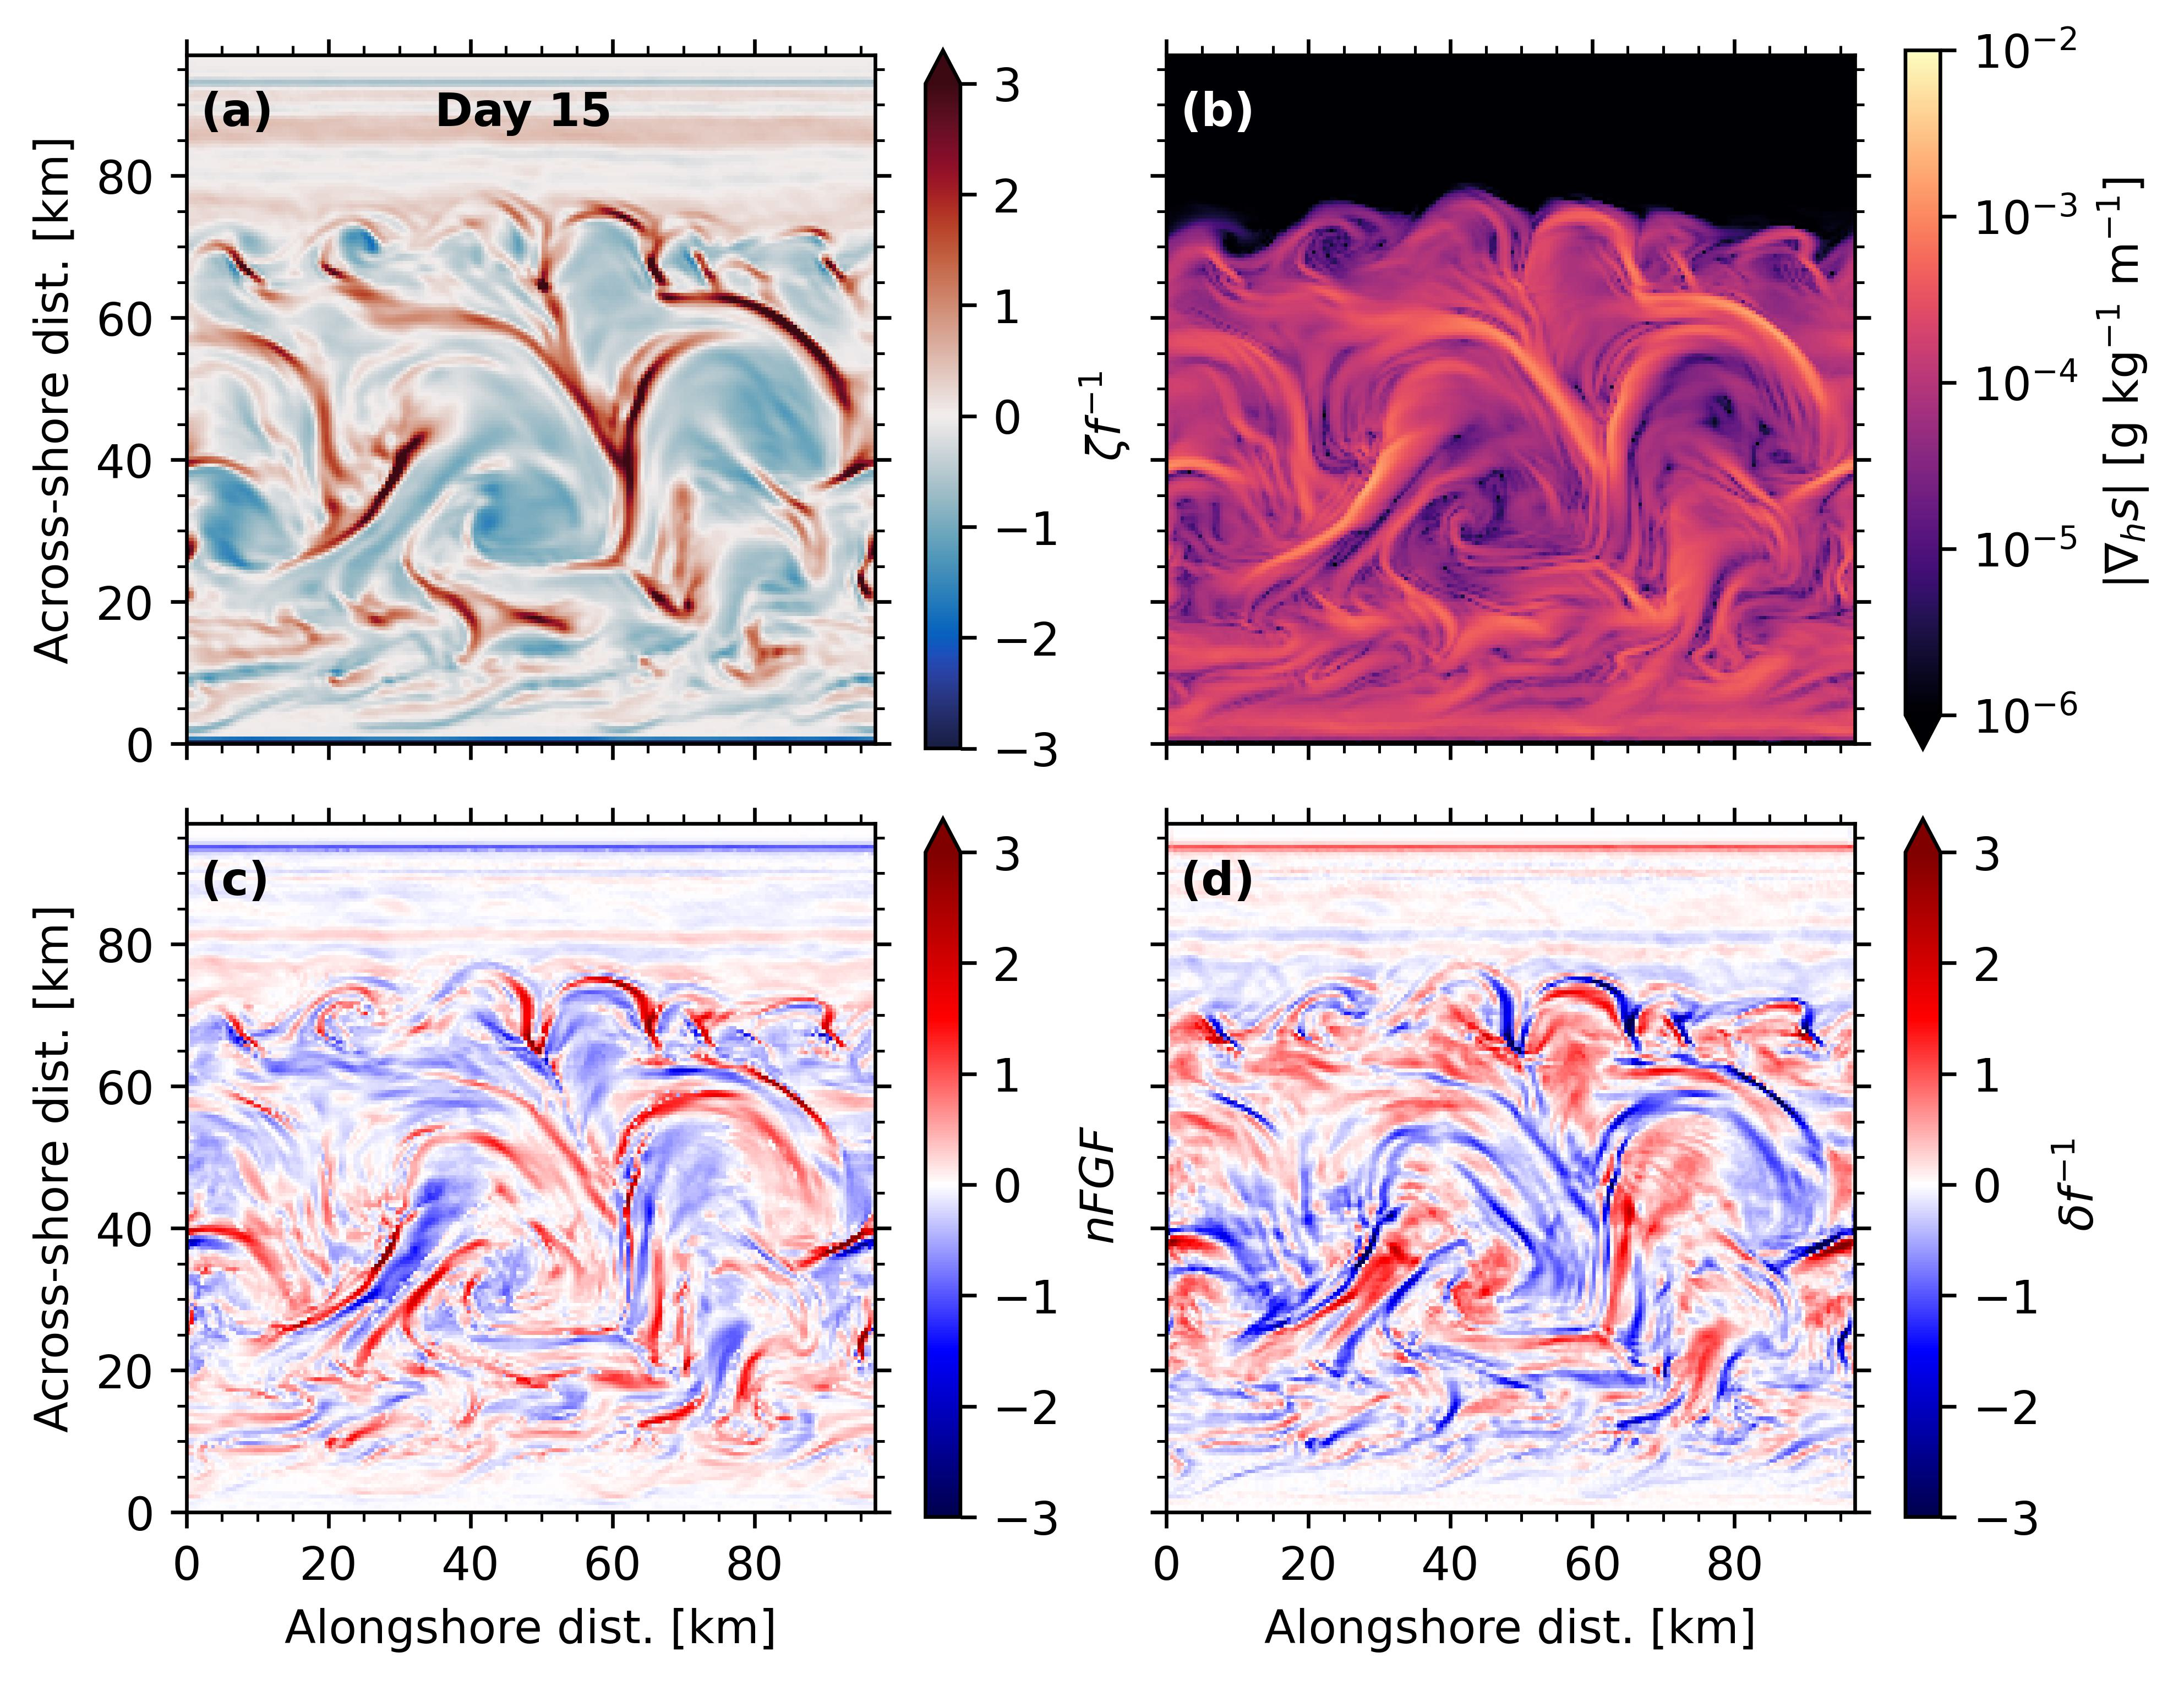
\includegraphics[width = \linewidth]{figures/shelfstrat_2024/surface_properties_day15.jpg}\\
    \caption{Plan view plots of surface $\zeta f^{-1}$ (a), $|\nabla_h s|$ (b), $nFGF$ (c), and $\delta f^{-1}$ (d) for the base case on day 15 as defined in text. $|\nabla_h s|$ values in (b) offshore of the instabilities are set to $10^{-6}$ g kg$^{-1}$ m$^{-1}$ to saturate the colorbar because they are poorly defined.}
    \label{fig:base_case_plan}
     \end{center}
\end{figure}

A statistical comparison between the realistic model and base case is shown with joint probability density functions (JPDFs) of $\mathcal{M}_{num}$ and $nFGF$ in the surface layer in Fig. \ref{fig:jpdf}. The absolute value of $\mathcal{M}_{num}$ is taken to account for negative values. The cyan line marks the maximum probability of $\mathcal{M}_{num}$ in each $nFGF$ bin sorted by active fronts ($\zeta f^{-1}>1$). The yellow line displays all cells in the surface layer. The TXLA model JPDF was constructed using a week of model output where the eddies are relatively unperturbed by various forcing (compare Fig. \ref{fig:txla_snap} to Fig. 2 of \citet{Schlichting23}). 

\begin{figure}[t!]
    \begin{center}
    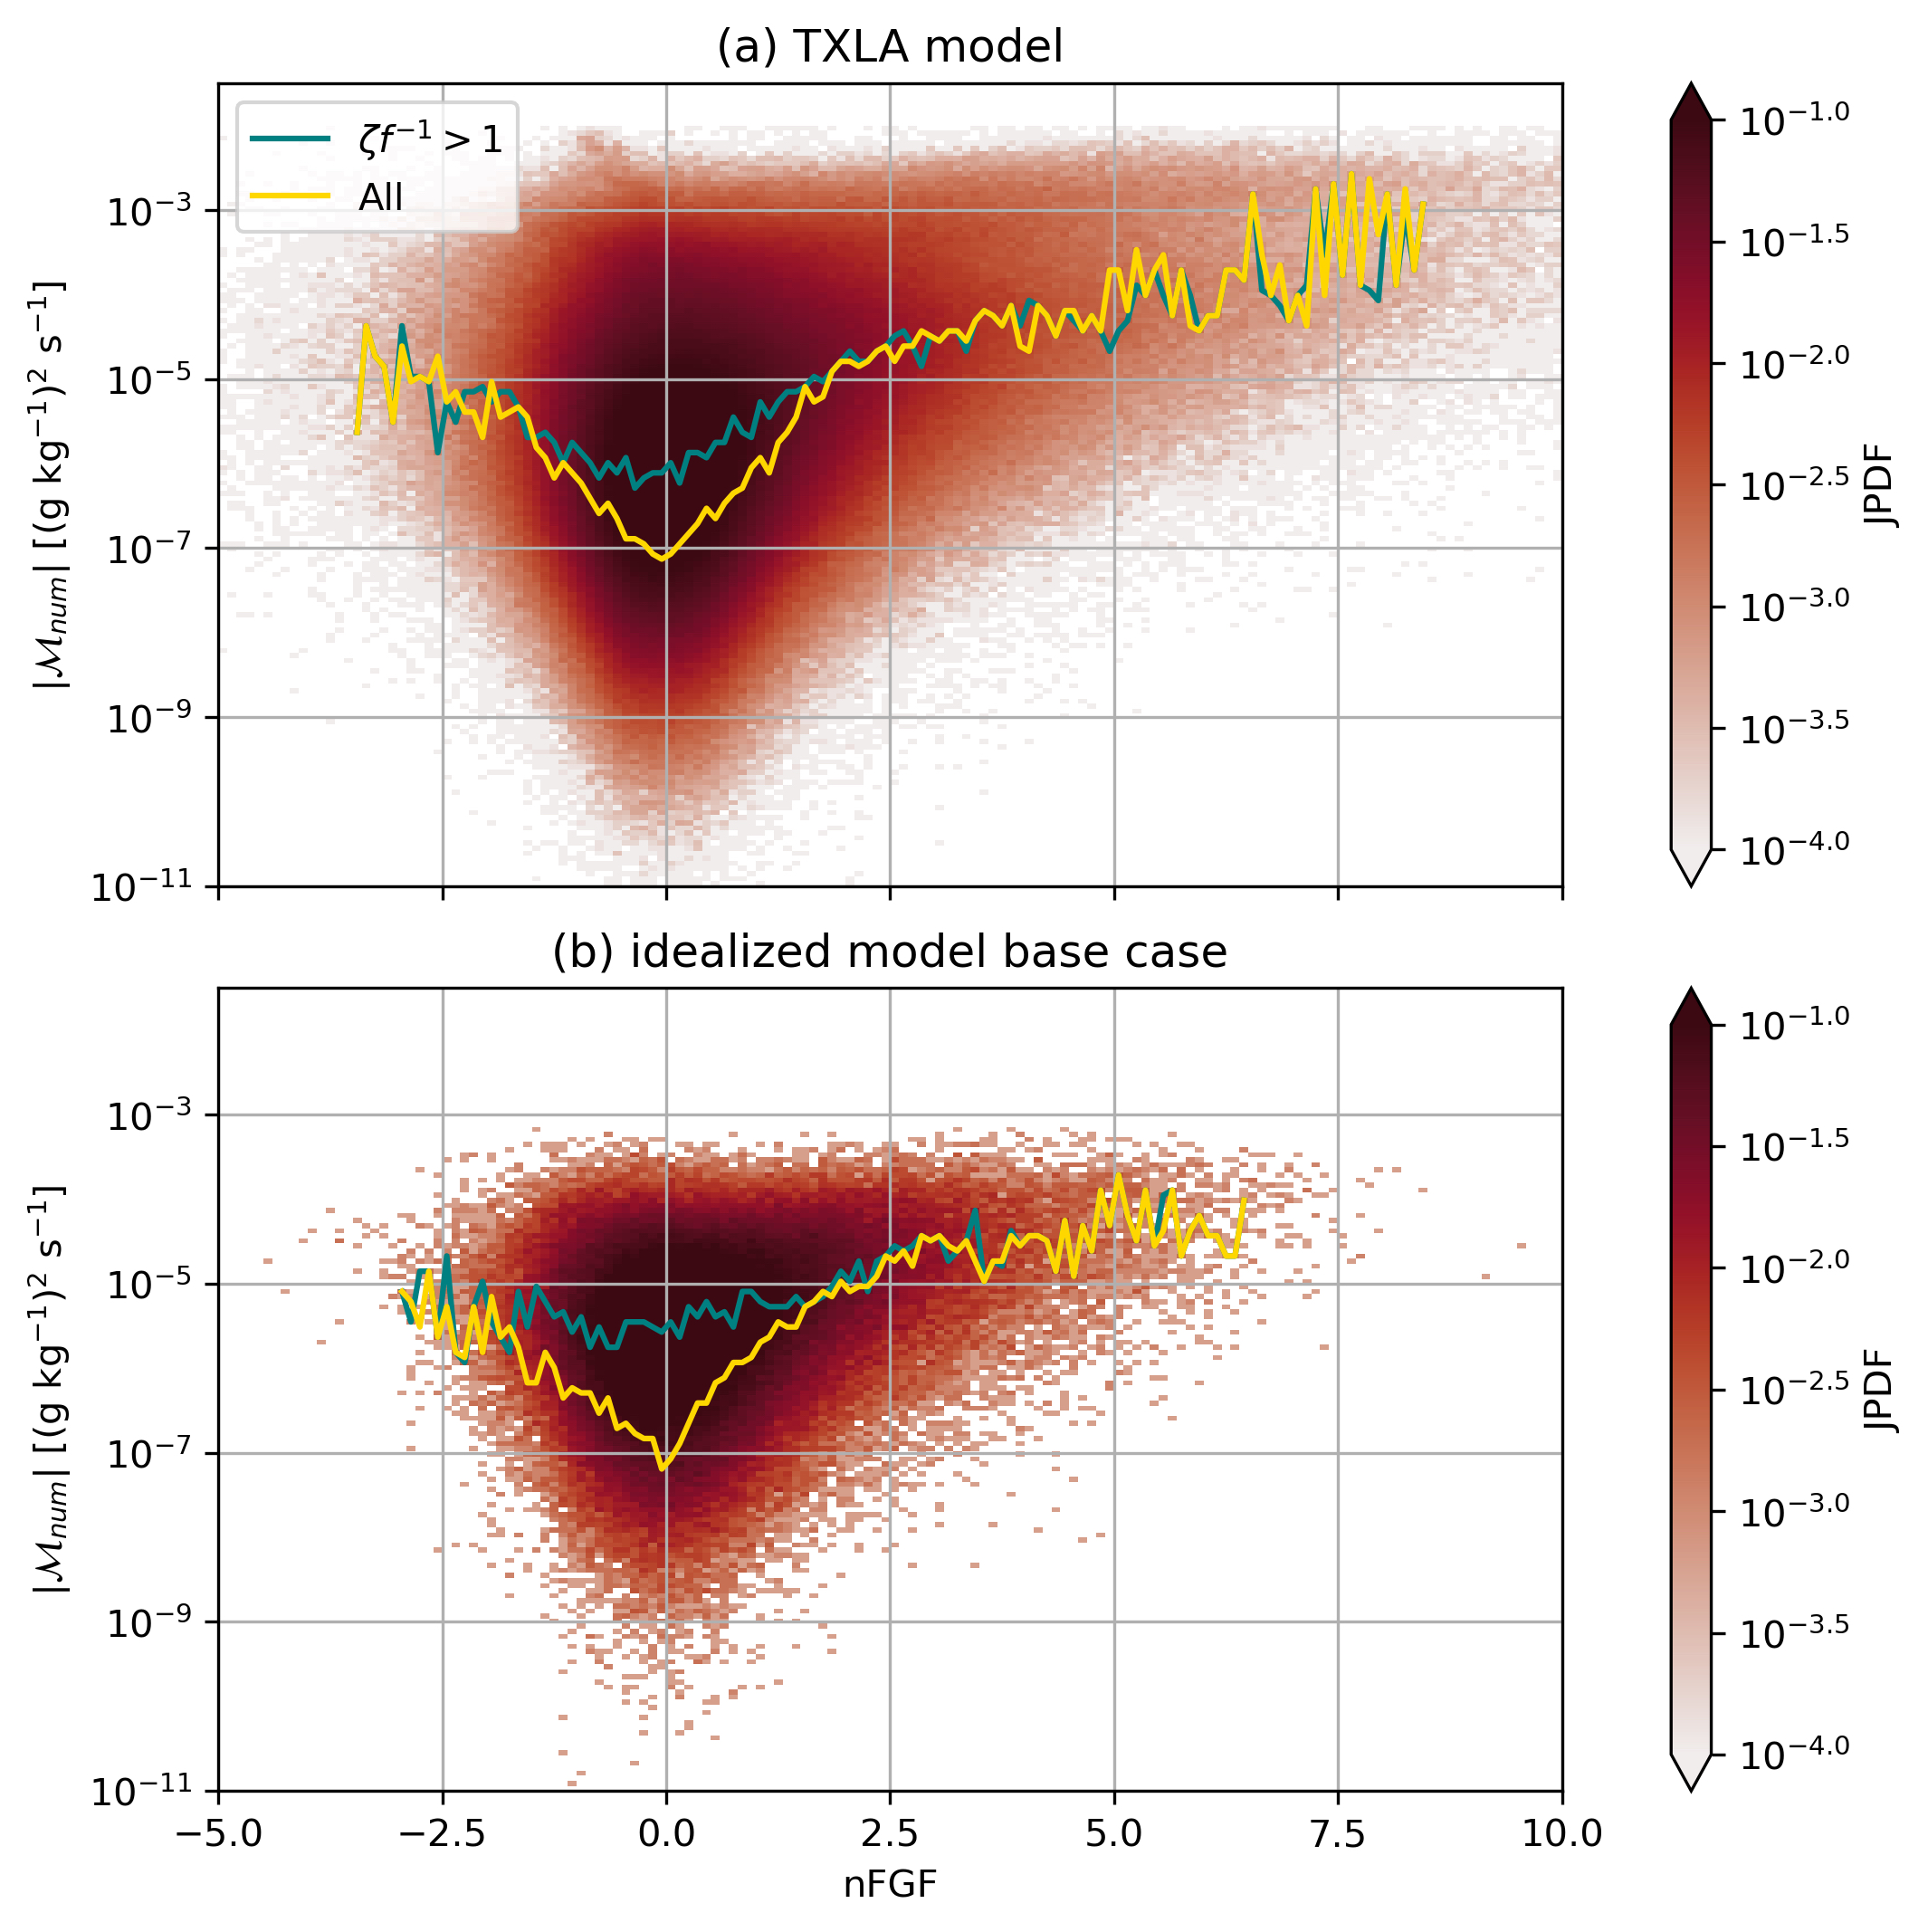
\includegraphics[width = 0.9\linewidth]{figures/shelfstrat_2024/txla_shelfstrat_jpdf.jpg}\\
    \caption{Joint probability density function (JPDF) of surface $|\mathcal{M}_{num}|$ and $nFGF$  for the realistic model from June 20-26, 2010 (a). The cyan line highlights the maximum value of the JPDF in each $nFGF$ bin sorted by active fronts ($\zeta/f>1$)  and the yellow line marks the same calculation but the entire surface layer. (b) Same as (a), but for the base case from days 7.5-15 inshore of the initially stratified region.  In (b), we removed the first three across-shore boundary points near the coastal wall due to strong convergence and divergence regions generated by the winds.}\label{fig:jpdf}
     \end{center}
\end{figure}

Several conclusions are drawn from Fig. \ref{fig:jpdf}: 1) the strongest occurrences of frontogenesis produce the sharpest horizontal salinity gradients and thus the strongest $\mathcal{M}_{num}$, 2) numerical mixing experiences the largest variability when frontogenesis and frontolysis are weak (i.e., $nFGF \sim [-1,1]$), which constitutes the majority of grid cells in the surface layer, 3) frontogenesis and frontolysis in the base case is representative of the realistic model, and 4) $nFGF$ is skewed towards frontogenesis. An interesting result is that $\mathcal{M}_{num}$ is significant even for strongly frontolytic processes. This reinforces the idea that lateral tracer gradients are a dominant parameter modulating $\mathcal{M}_{num}$, even if those gradients are being instantaneously weakened. In addition, the base case features smaller $\mathcal{M}_{num}$ and $nFGF$ ranges due to coarser lateral resolution and a smaller salinity range (see Section \ref{sec:model_setup}). The impacts of lateral resolution on $\mathcal{M}_{num}$ are further elucidated by cyan lines, where weak frontogenesis and frontolysis feature $\mathcal{M}_{num}$ maximum in each $nFGF$ bin (Fig. \ref{fig:jpdf} b) about half an order of magnitude stronger than the same range for the realistic model (Fig. \ref{fig:jpdf} a). In addition, the maximum $\mathcal{M}_{num}$ in each $nFGF$ bin for the entire surface layer converges to same quantity sorted by fronts when $|nFGF| \sim 2$. While determining a proper scaling between $\zeta f^{-1}$ and $nFGF$ or $\delta f^{-1}$ is beyond the scope of this paper, it makes intuitive sense for strong fronts and eddies to be present in regions of strong frontogenesis and frontolysis. 

\subsection{Tracer advection experiments} \label{sec:tadv_exp}
Next, we study the sensitivity of the base case with three tracer advection schemes available in the COAWST source code. The schemes used are MPDATA \citep{smolarkiewicz1984fully, Smolarkiewicz_1998}, third-order upwind in the horizontal with a vertical fourth-order centered scheme \citep[U3HC4,][]{shchepetkin1998quasi}, and third high-order spatial interpolation at the middle temporal level with a total variation diminishing scheme \cite[HSIMT,][]{wu2010advection, wu2023evaluation}. MPDATA is second order accurate but features anti-diffusive properties. \citep{Kalra_2019} also studied the sensitivity of $\mathcal{M}_{num}$ and $\mathcal{M}_{phy}$ in four idealized test cases using COAWST with the same schemes. An overview of the schemes can be found in their Section 2.2 and references therein.

We conduct 30 day ensemble runs of the base case by varying the model bathymetry to ensure differences between advection schemes are robust. That is, 1\% random noise added to the bathymetry is regenerated for each ensemble member. 95\% confidence intervals of volume-integrated, ensemble-averaged energetics and mixing quantities are provided to characterize the variability (denoted with an overbar). All quantities in Fig. \ref{fig:tadv_vol_int} are smoothed with a 16 hour rolling mean (denoted with angle brackets) to remove the primary oscillations caused by the wind and improve readability. We used a larger across-shore domain (194 km) so the eddies never interact with boundary. Volume integration was performed from the coast to 97 km across-shore, which represents the boundary of the original domain. In addition, the eddies from several ensemble members approximately reach this location by Day 30 (Fig. \ref{fig:isohalines}). We deemed eight ensemble members sufficient to capture variability caused by changing the bathymetry noise, as shown by the confidence intervals of each quantity shown in Fig. \ref{fig:tadv_vol_int}. 

\begin{figure}[t!]
    \begin{center} 
    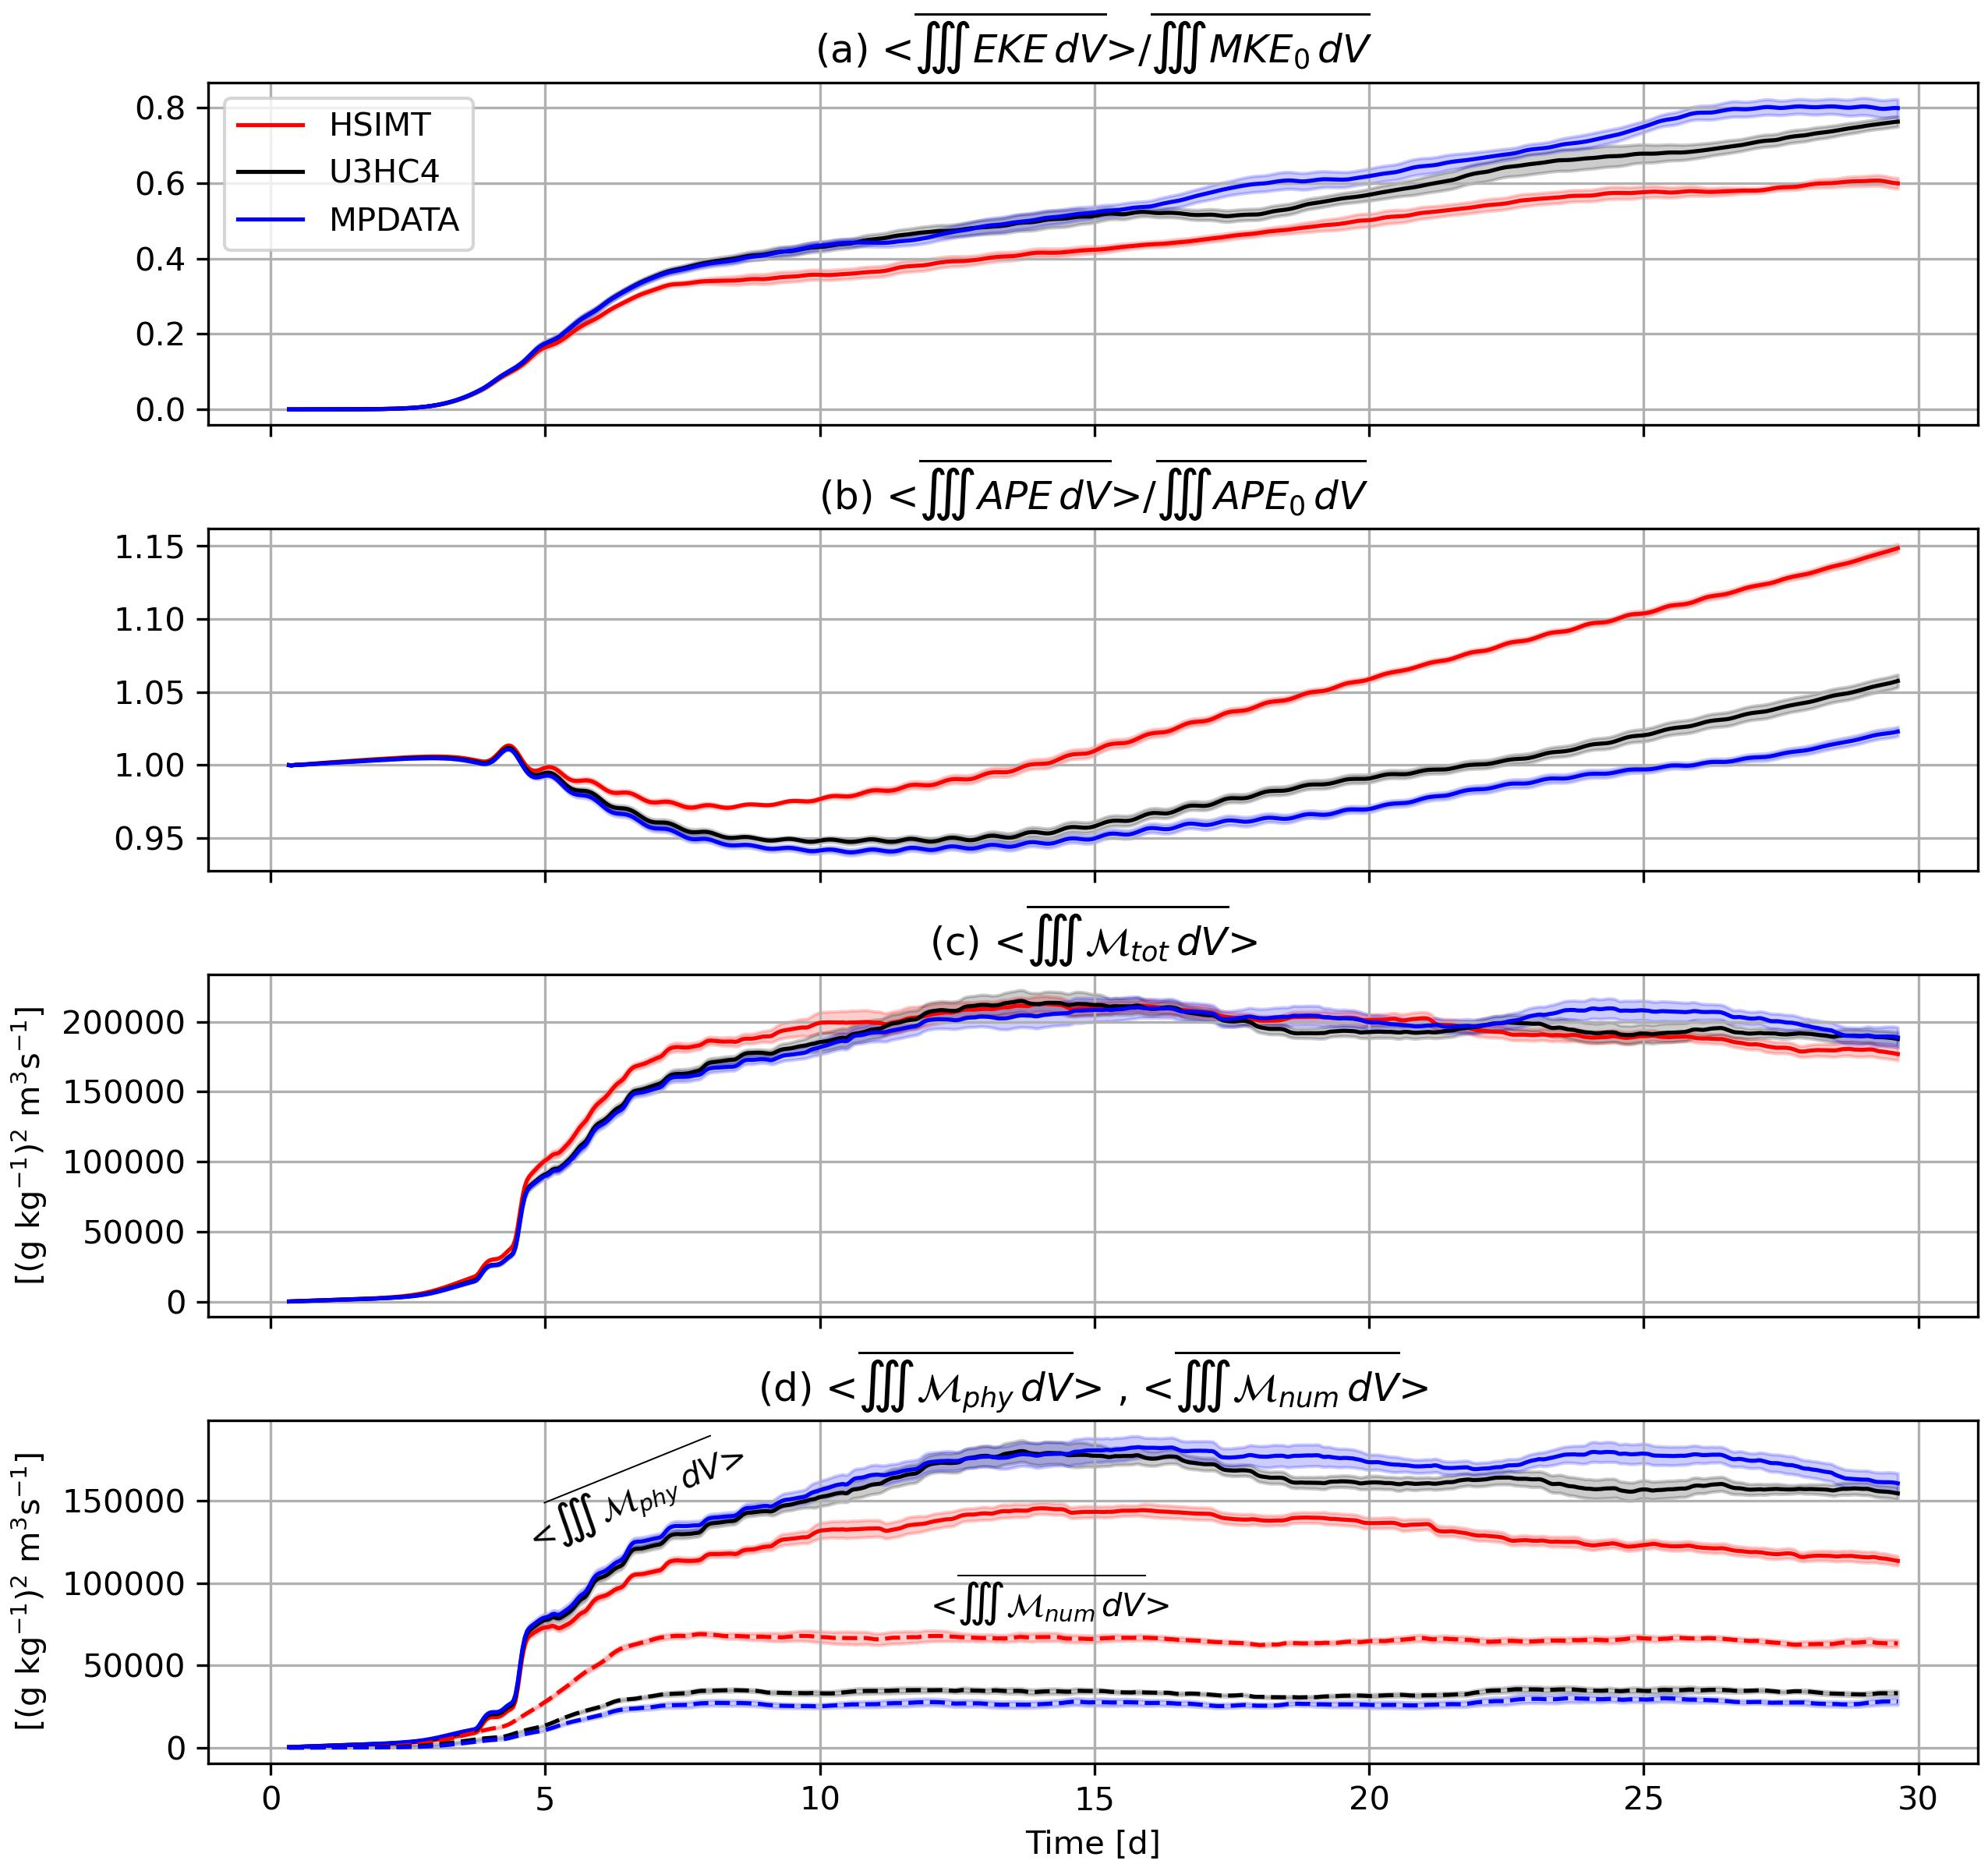
\includegraphics[width = 0.9\linewidth]{figures/shelfstrat_2024/tadvection_vol_int_ens.jpg}\\
    \caption{Time series of $EKE_{n,ens}$ (a), $APE_{n,ens}$ (b), $\mathcal{M}_{tot, ens}$ (c), and $\mathcal{M}_{phy,ens}$ and $\mathcal{M}_{num,ens}$ (d) as defined in text. The angle brackets denote a 16 hour rolling mean and the overline denotes an ensemble average. The shaded areas represent values within the 95\% confidence intervals about the ensemble means. In (d), $\mathcal{M}_{phy,ens}$ is shown with solid lines and $\mathcal{M}_{num,ens}$ is shown with dashed lines.} \label{fig:tadv_vol_int}
     \end{center} 
\end{figure}

We start with analysis of the double-averaged, volume-integrated $EKE$: 
\begin{equation}
    EKE_{n,ens} = \langle \overline{\iiint EKE \, dV }\rangle \left[\overline{\iiint MKE_0 \, dV}\right]^{-1}.
\end{equation}

Differences between schemes are detectable shortly after the eddies begin forming. HSIMT features the lowest $EKE_{n,ens}$ throughout the simulation. By Day 30, HSIMT's ensemble-averaged $EKE_{n,ens}$ is nearly 25\% less than the other schemes. The confidence intervals of $EKE_{n,ens}$ between U3HC4 and MPDATA overlap for much of the simulation, requiring further analysis to identify whether the numerical schemes are significantly different. 

Following \citet{Hetland_2017}, we compare the tracer advection schemes using the available potential energy ($APE$), which is defined as 
\begin{equation}
    APE = -\rho_0 b^\prime z \, , 
\end{equation}

where $b^\prime = b-b_{ref}$ is the buoyancy anomaly with reference buoyancy $b_{ref}$. Here, $b = -g(\rho_{0}-\rho)\rho_0^{-1}$ with $\rho_0=1025$ kg m$^{-3}$. $b_{ref}$ is defined using the temperature-dependent part of Eq. \ref{eqn:EOS} so the across-shore buoyancy gradient is zero. $APE$ also has contributions from the sea surface height anomalies, however, these were determined to be negligible \cite[not shown, see Appendix B of][]{Hetland_2017}. %\citep<Regional Ocean Modeling Systems, ROMS,>[]{shchepetkin2005regional}

$APE$ can be directly related to the isopycnal slope \citep{brink2016continental1, brink2016continental2}. As baroclinic instabilities relax the mean flow, the slope of the initially tilted isopycnals is reduced \citep{Hetland_2017, zhang2018study}. A less developed eddy field will feature steeper isopycnals in the initially stratified region and more $APE$, corresponding to bottom isohalines (and isopycnals) more similar to the initial conditions. A more developed eddy field will feature bottom isohalines that have moved closer to the coast and less $APE$. Regarding the surface salinity structure, a more developed eddy field will feature isohalines that extend further offshore. This can be visualized qualitatively in Fig. \ref{fig:isohalines}, which depicts the ensemble members with the highest $EKE_n$ on Day 30 for each advection scheme.
\begin{figure}[t!]
    \begin{center}
    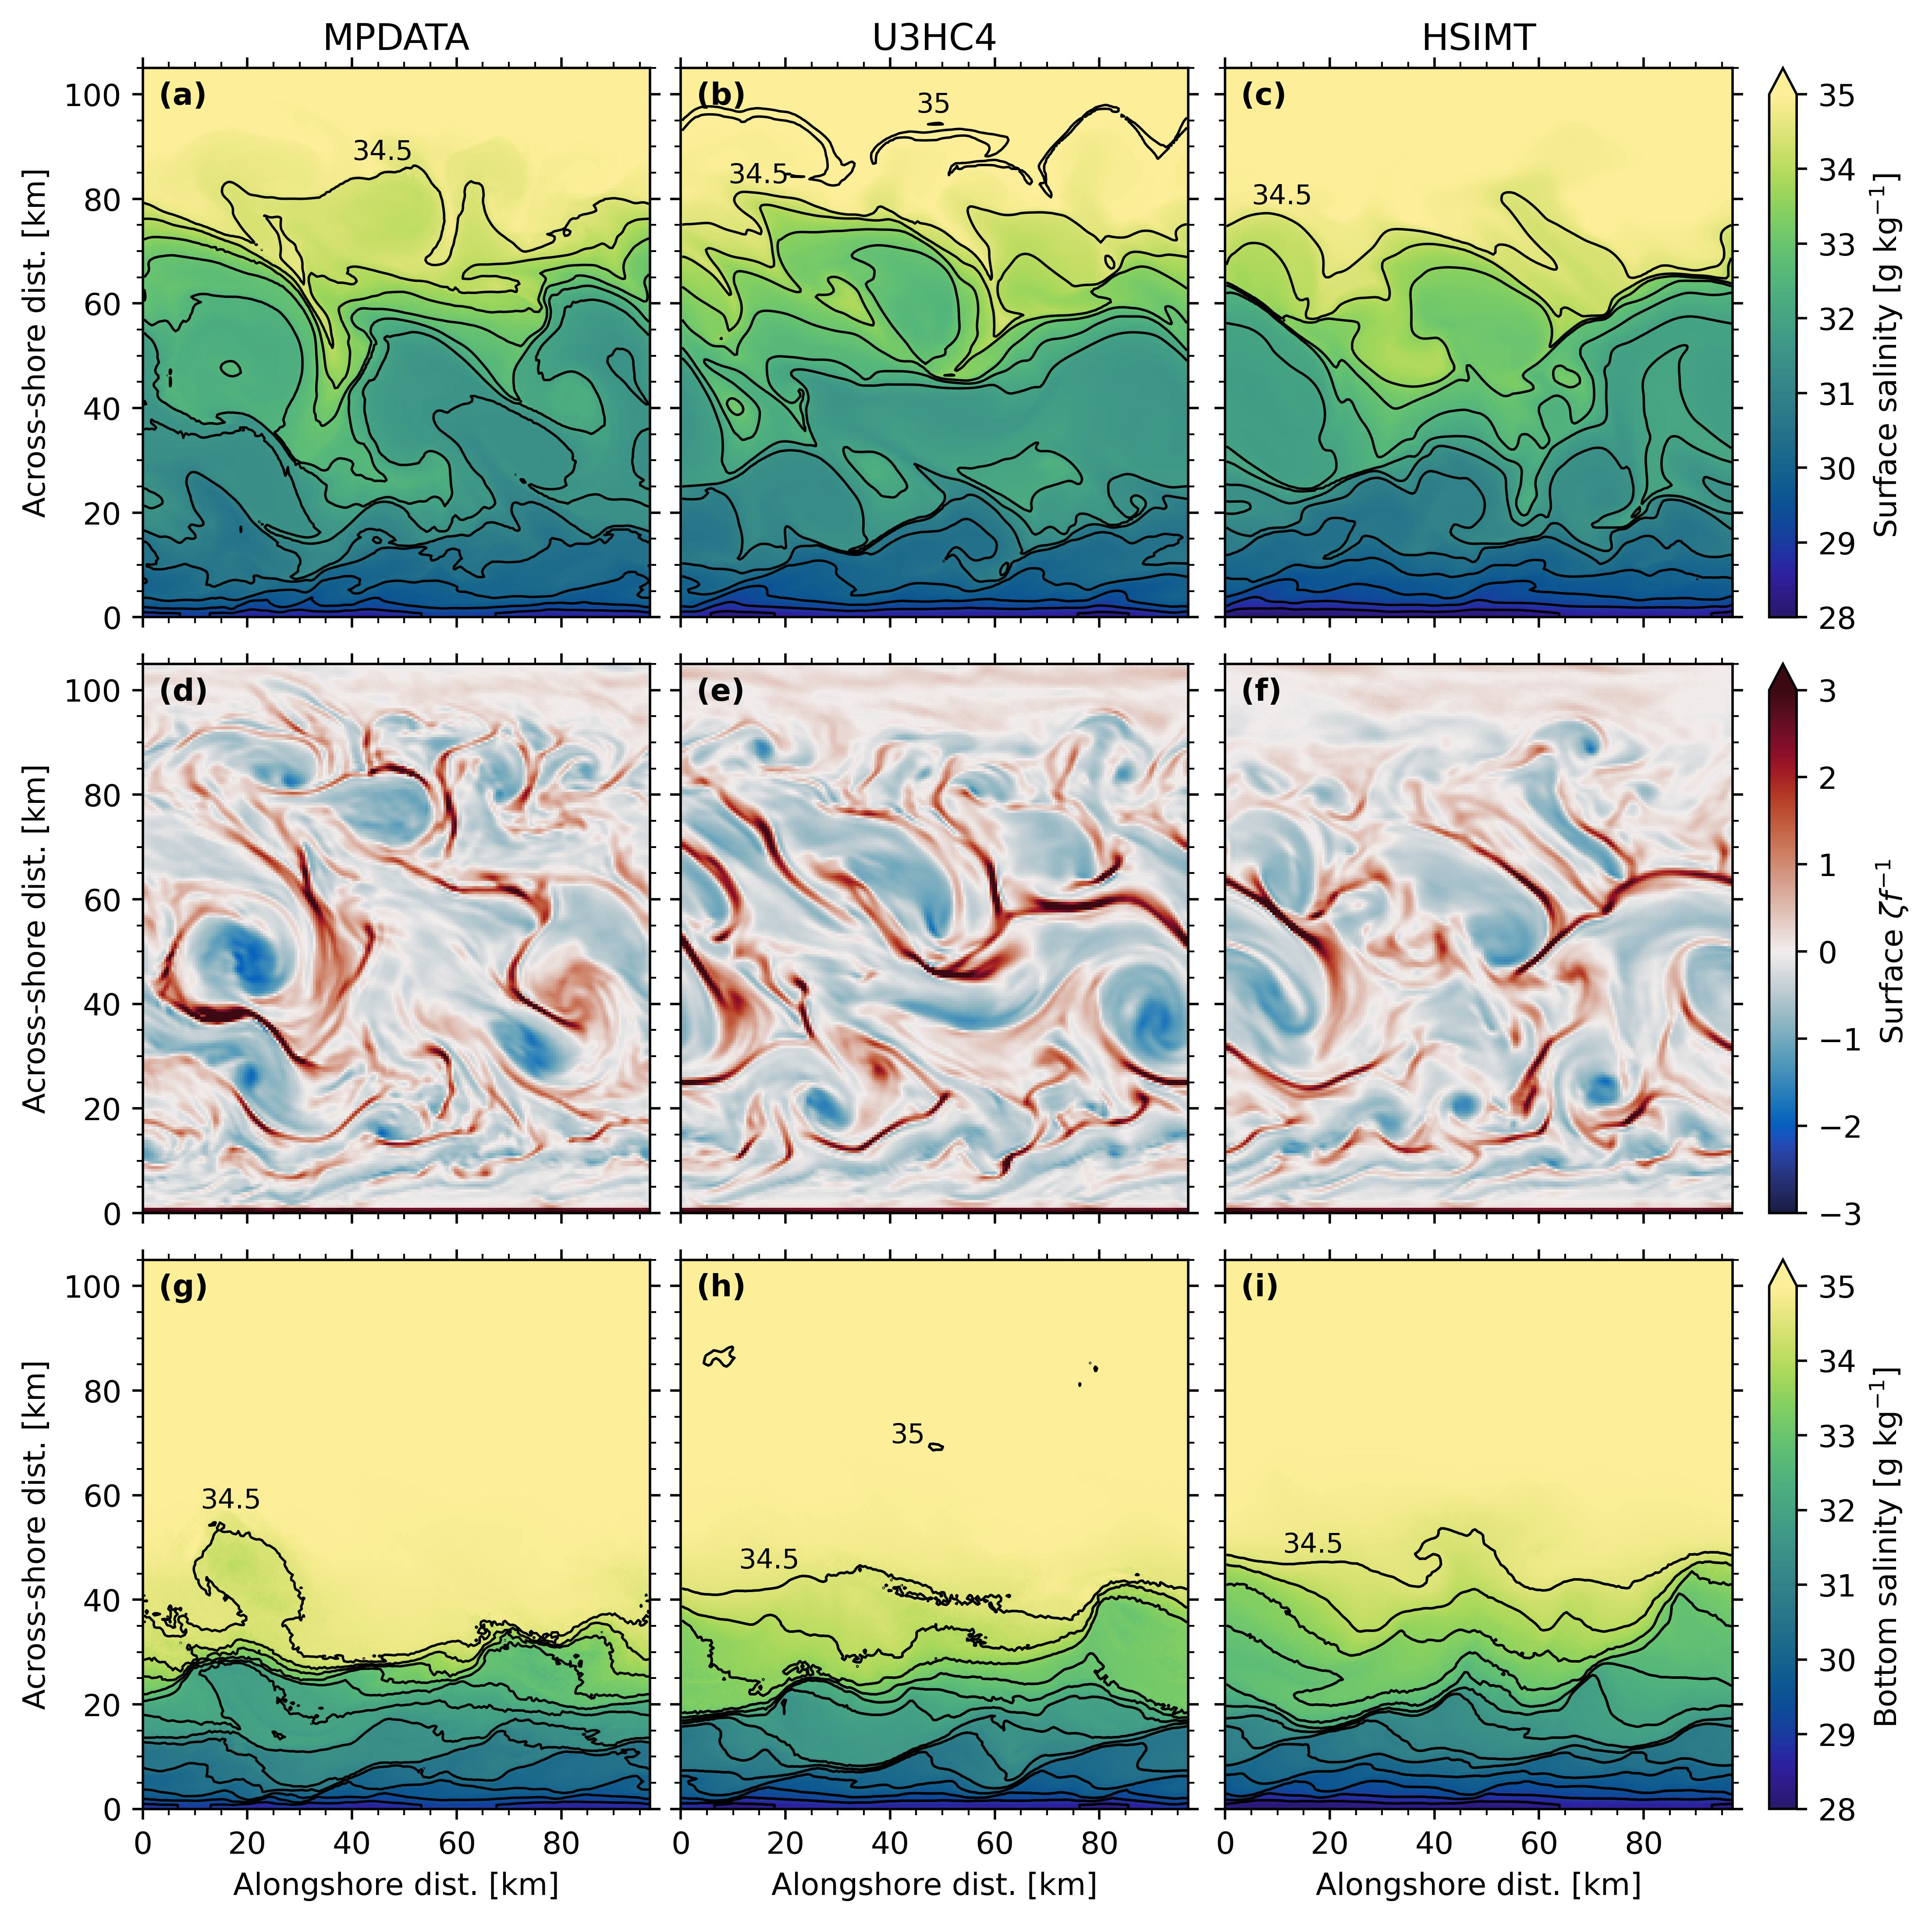
\includegraphics[width = 0.9\linewidth]{figures/shelfstrat_2024/shelf_dx_500_tadv_dt_30_day_30.jpg}\\
    \caption{Snapshots of surface salinity (a-c), surface $\zeta f^{-1}$ (d-f), and bottom salinity (g-i) on Day 30. Each column represents a different tracer advection scheme ensemble member with the largest $EKE_n$ on Day 30. Isohalines are shown every 0.5 g kg$^{-1}$ over the range of the colorbar in (a-c) and (g-i). The 35 g kg$^{-1}$ contours in the U3HC4 ensemble member are spurious.} \label{fig:isohalines}
     \end{center} 
\end{figure}

The volume-integrated double-averaged $APE$ is normalized by its initial value $APE_0$:
\begin{equation}
    APE_{n, ens} = \langle \overline{\iiint APE \, dV} \rangle \left[\overline{\iiint APE_0 \,dV}\right]^{-1}.
\end{equation}
$APE_{n, ens}$ is shown in Fig. \ref{fig:tadv_vol_int} (b) for each scheme and is consistent with arguments posed above. By day five, HSIMT has more $APE_{n, ens}$ than the other schemes and this grows with respect to time. U3HC4 has more $APE_{n, ens}$ than MPDATA for the entire simulation, although these differences remain marginal until day 15. The $APE_{n, ens}$ for all schemes decreases below their initial values, plateaus, then eventually rise above their initial values. The $APE_{n, ens}$ decreases as the isopycnal slope is reduced in the initially stratified region. Later increases in $APE_{n, ens}$ are caused by wind-induced mixing offshore of the eddy field where the isopycnal slope is controlled by temperature. There, wind mixing increases the isopycnal slope, which compensates for the $APE_{n, ens}$ decrease in the initially stratified region. If volume-integration were performed inshore of the initially stratified region, $APE_{n, ens}$ would continuously decline below its initial values (not shown). 

While the $EKE_{n, ens}$ remains similar between U3HC4 and MPDATA, differences in their bottom salinity structure (Fig. \ref{fig:isohalines} g-i) qualitatively support the idea that higher numerical mixing in U3HC4 reduces the amount of energy that can be extracted from the horizontal density gradient. That is, MPDATA isohalines are more pinched coast to the coast than U3HC4. Differences in the surface salinity structure also validate this argument (Fig. \ref{fig:isohalines} a-c) , with MPDATA experiencing the furthest offshore development of the 34.5 g kg$^{-1}$ isohaline. U3HC4 features spurious 35 g kg$^{-1}$ isohalines throughout the water column because the scheme is non-monotonic.  The argument that MPDATA and U3HC4 produce more-developed eddies is further supported with surface $\zeta f^{-1}$ (Fig. \ref{fig:isohalines}). In the end, the differences between U3HC4 and MPDATA are marginal. U3HC4 locally produces the sharpest fronts, but PDFs of $\zeta f^{-1}$ (not shown) are nearly identical.

Bulk values and ratios of the decomposed, ensemble-averaged integrated mixing quantities are shown in Tab. \ref{tab:mixing_tadv}. For example, the double-averaged, integrated total mixing is written as:
\begin{equation}
    \mathcal{M}_{tot,ens} = \langle \overline{\iiint \mathcal{M}_{tot} \, dV } \rangle
\end{equation}
and likewise for the physical $\mathcal{M}_{phy, ens}$ and numerical mixing $\mathcal{M}_{num,ens}$. HSIMT runs have substantially more numerical mixing than the other schemes and moderately less physical mixing. $\mathcal{M}_{phy,ens}$ constitutes 86\% of $\mathcal{M}_{tot,ens}$ for MPDATA, 83\% for U3HC4, and 66\% for HSIMT. $\mathcal{M}_{tot,ens}$ is very similar between the different advection schemes. 

\begin{table}[t]
\caption{Sensitivity of ensemble-averaged mixing quantities to the tracer advection scheme. Ratios of bulk (denoted by $\Sigma$) volume-integrated physical, numerical, and total mixing inshore of 97 km from Days 7.5-30. Note these are \textit{not} smoothed with a 16 hour rolling mean. Bulk values have units of 10$^7$(g kg)$^2$ m$^3$s$^{-1}$.} \label{tab:mixing_tadv}
\begin{center}
\begin{tabular}{cccccc}
\hline
Scheme & $\Sigma \mathcal{M}_{phy,ens}$& $\Sigma \mathcal{M}_{num,ens}$& $\Sigma \mathcal{M}_{tot,ens}$& $\mathcal{M}_{phy,ens}/\mathcal{M}_{tot,ens}$ & $\mathcal{M}_{num,ens}/\mathcal{M}_{tot,ens}$\\
\hline
MPDATA& 9.90& 1.59& 11.49& 0.86& 0.14  \\ 
U3HC4& 9.39& 1.98& 11.37& 0.83& 0.17 \\
HSIMT& 7.66& 3.88& 11.54& 0.66& 0.34 \\
\hline
\end{tabular}
\end{center}
\end{table}

Instantaneously, $\mathcal{M}_{num,ens}$ is larger in HSIMT runs relative to other schemes at all times. These results suggest that as instabilities form, the increased $\mathcal{M}_{num,ens}$ suppresses instability growth by preventing the release of $APE$. Weaker eddies decrease the relative amount of $\mathcal{M}_{phy,ens}$ because they do not penetrate as deeply into the water column. Therefore, the impacts of $\mathcal{M}_{num,ens}$ on the larger-scale flow are similar to larger-scale models and \textit{not} like an implicit LES discussed in Section 1. In other words, the solution is sensitive to the type of mixing that occurs, even if the $\mathcal{M}_{tot,ens}$ is similar between different advection schemes.

Finally, we provide quantitative estimates of the differences in salinity structure between the advection schemes. This is done using cross-sections of alongshore- and ensemble-averaged salinity ($\overline{\overline{s}}$) on days 7.5 and 30 for MPDATA and the relative differences $\Delta \overline{\overline{s}}$ with other schemes are shown in Fig. \ref{fig:cs_salt}. This allows us to examine whether the differences in salinity structure shown in Fig. \ref{fig:isohalines} are robust and not due to analysis of the highest $EKE$ ensemble members. Alongshore- and ensemble-averaged isopycnals are also overlaid every 0.5 kg m$^{-3}$. The 1027 kg m$^{-3}$ isopycnal approximately represents the boundaries of the salinity stratified region (Fig. \ref{fig:cs_salt} a).

\begin{figure}[t!]
    \begin{center}
    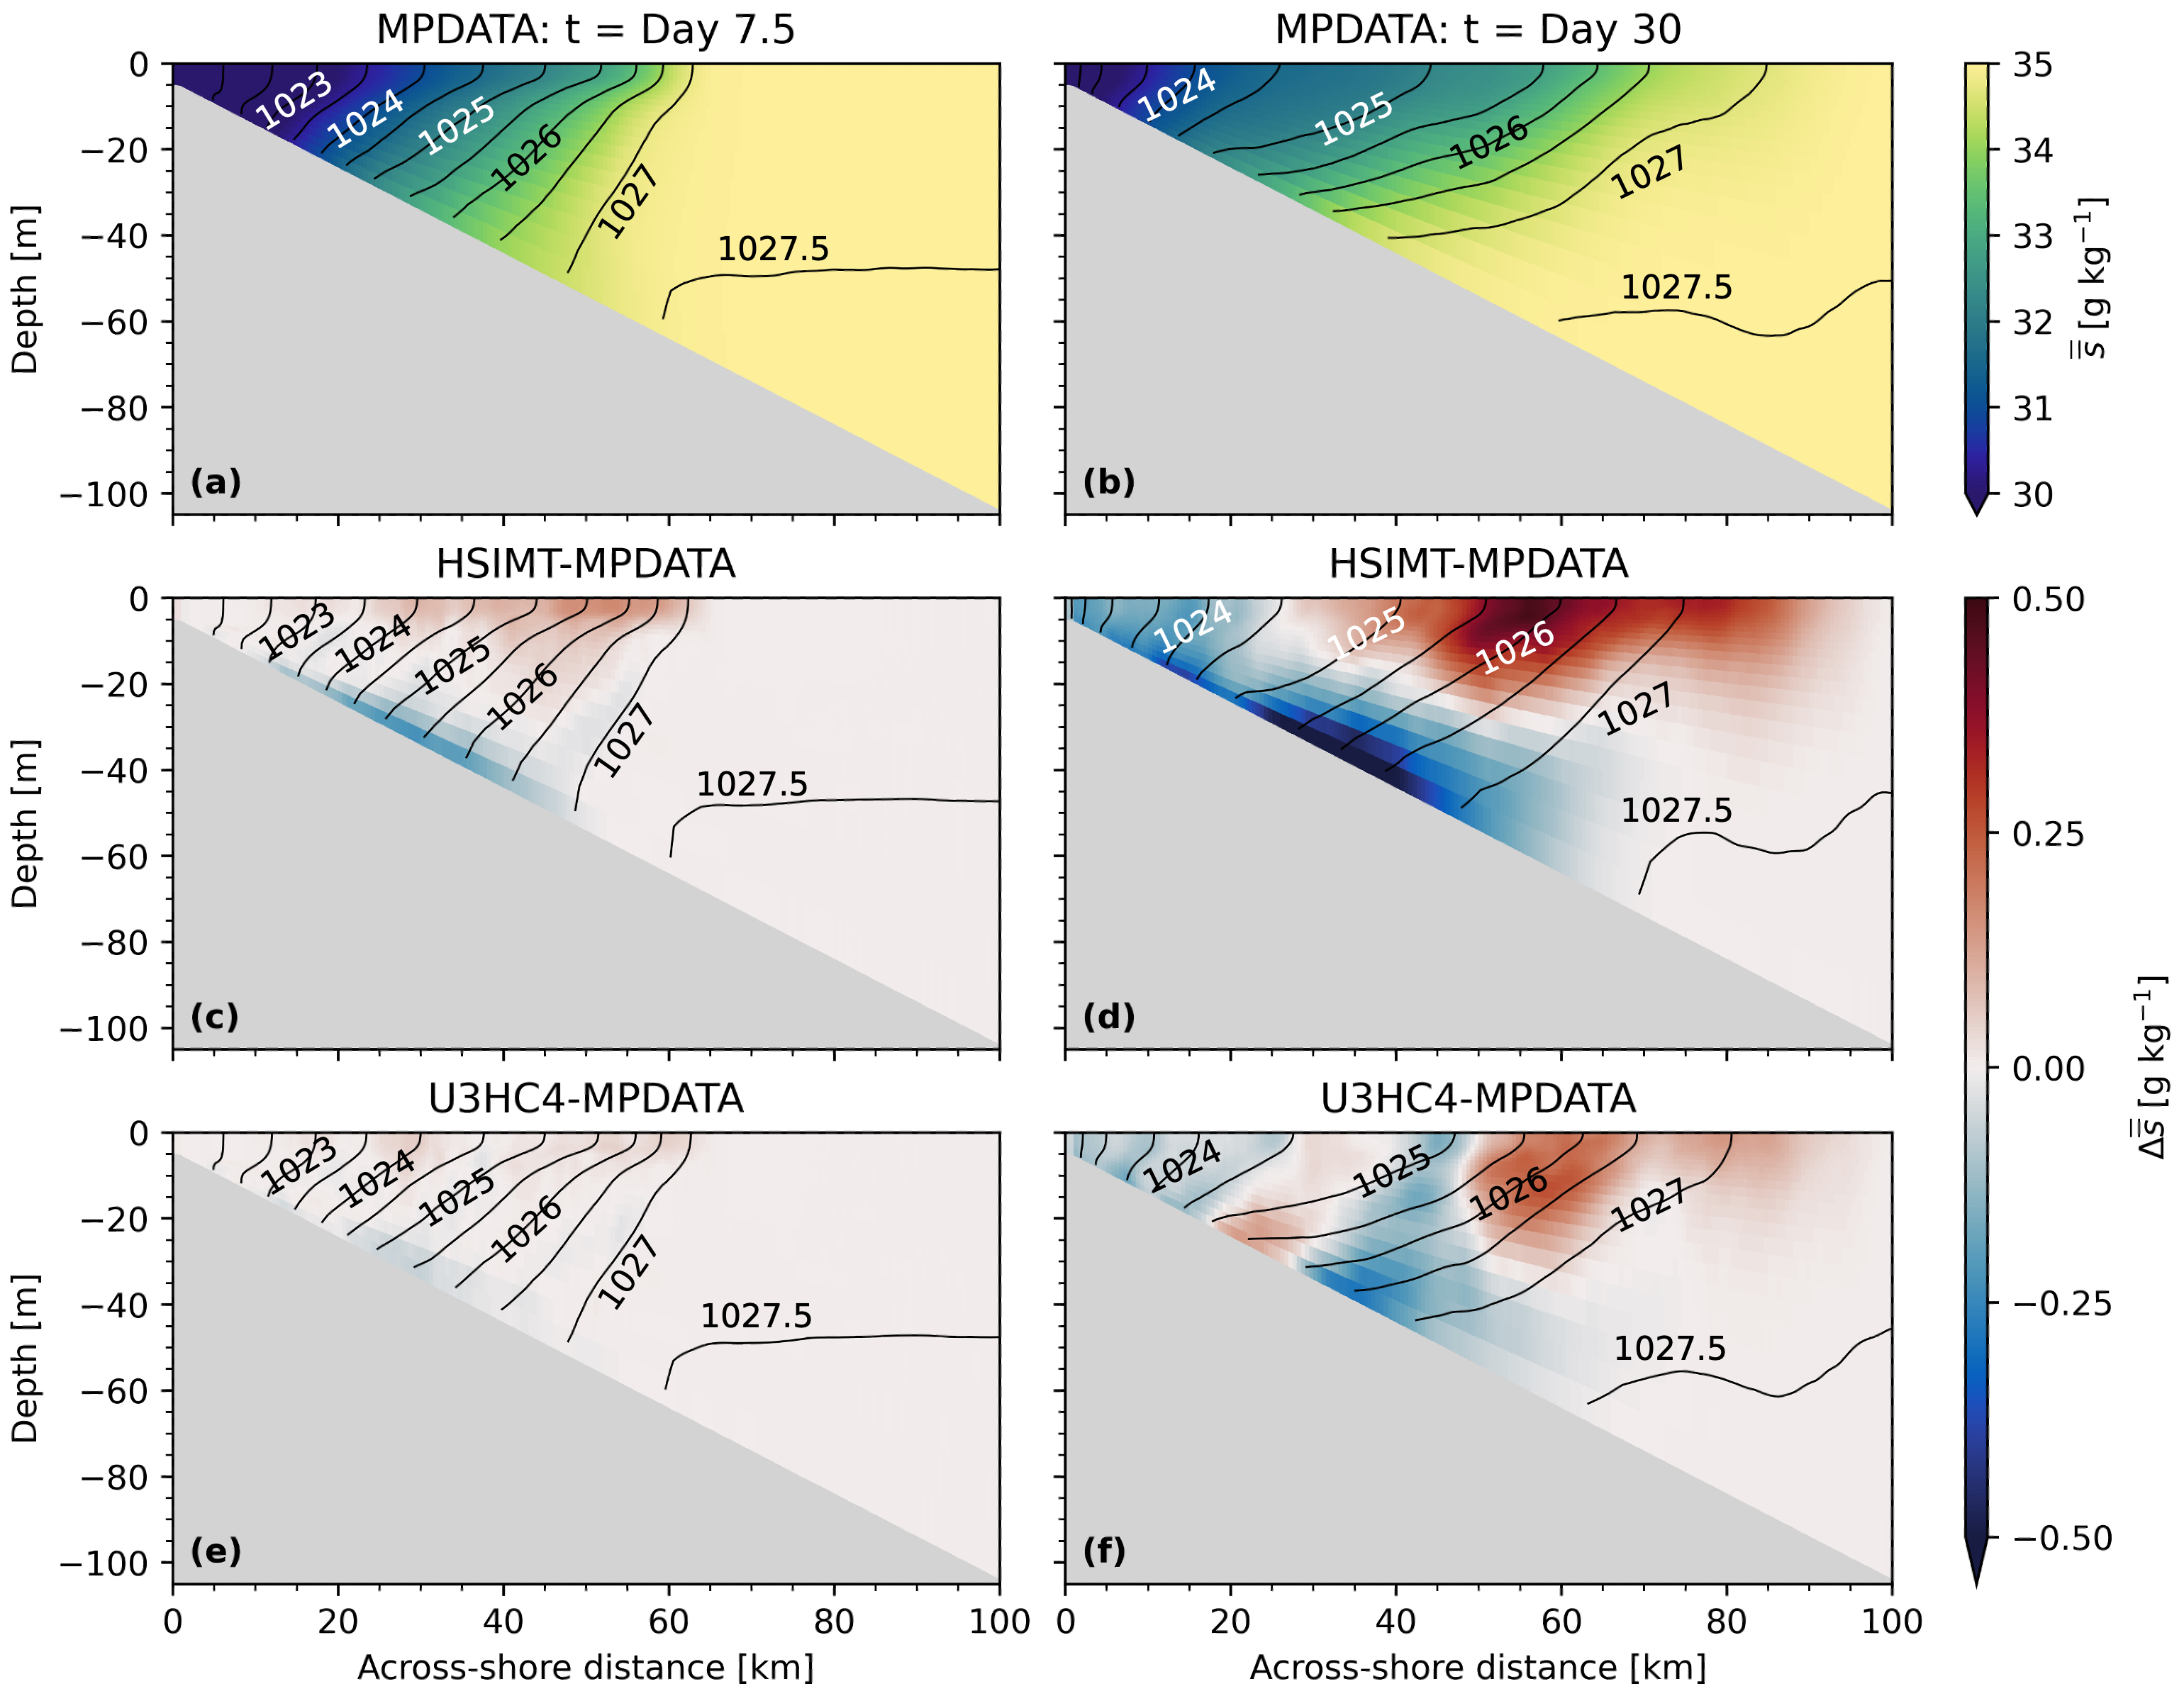
\includegraphics[width = \linewidth]{figures/shelfstrat_2024/tadv_cs_salt_isopyc.jpg}\\
    \caption{Cross-sections of alongshore- and ensemble- averaged salinity (indicated by double overline) for MPDATA on Days 7.5 (a) and 30 (b). Relative differences between the same quantities for HSIMT (c-d) and U3HC4 (e-f). Isopycnals are overlaid every 0.5 kg m$^{-3}$ for each scheme. Note the bathymetry noise is smoothed by the averaging, so the isopycnals do not appear to reach the seafloor.} \label{fig:cs_salt}
     \end{center} 
\end{figure}

On day 7.5, $\Delta \overline{\overline{s}}$ between HSIMT and MPDATA is small, with a two layer structure that is fresher near the bottom and saltier from the middle of the water column to the surface (Fig. \ref{fig:cs_salt} c).  The differences between U3HC4 and MPDATA are lesser, and $\Delta \overline{\overline{s}}$ is slightly fresher towards the bottom inshore of the initially stratified region and saltier near the surface (Fig. \ref{fig:cs_salt} e). Differences in isopycnal structure between schemes are marginal on day 7.5, but by day 30, the mean isopycnal slope has reduced for all advection schemes. The surface position of the 1027 kg m$^{-3}$ isopycnal is approximately 10 km further offshore in the MPDATA case than in the HSIMT case and five km further offshore in the  MPDATA case than in the U3HC4, consistent with previous arguments. 

On day 30, $\Delta\overline{\overline{s}}$ between HSIMT and MPDATA is saltier by up 0.5 g kg$^{-1}$ in the upper half of the water column offshore of 30 km. In the lower half of the water column, $\Delta\overline{\overline{s}}$ is fresher by over -0.75 g kg$^{-1}$ close to the bottom. Inshore of 30 km, $\Delta \overline{\overline{s}}$ is persistently fresher. Regarding U3HC4, $\Delta \overline{\overline{s}}$ is smaller in magnitude than HSIMT nearly everywhere except for a saltier band that extends diagonally through the water column from 15-40 km.

\section{Discussion} \label{sec:discussion}

Previous studies suggest numerical mixing impacts the larger-scale flow and tracer structure differently than physical mixing in simulations of estuarine and coastal flows using primitive equation models \citep{fofonova2021plume, Kalra_2019, karna2016evaluation, Ralston_2017}. However, these studies come with one of the following caveats or challenges: 1) mixing is not quantified directly or online \citep{fofonova2021plume, karna2016evaluation}, 2) the domains are highly idealized \citep{fofonova2021plume, Kalra_2019}, and 3) quantitative relationships between numerical mixing and model skill in realistic domains requires an extensive array of field observations \citep{karna2016evaluation, Ralston_2017}. The current study is novel because we explicitly quantify the numerical mixing in an idealized domain that is able to realize a complex ocean state that resembles conditions in a realistic simulation. While the base case is not fully realistic due to the idealized bathymetry and lack of river forcing, eddy structure (Fig. \ref{fig:base_case_plan}) and frontogenesis/frontolysis (Fig. \ref{fig:jpdf}) are representative of the realistic model. The idealized domain allows for a large ensemble of simulations, as well as clear metrics for comparisons across the ensemble through alongshore averages.

A primary result of our study is that excessive numerical mixing can damp the release of $APE$ by suppressing submesoscale baroclinic instabilities. To demonstrate this, we varied numerical mixing through the choice of advection scheme, each with different numerical mixing, in order to relate an alongshore average state to the magnitude of numerical mixing. Even though simulations using all of the different advection schemes are submesoscale eddy-resolving, in that they all have qualitatively similar energetic eddy fields, $\mathcal{M}_{num}$ impacts the larger-scale flow and tracer fields in such a way that simulations with higher numerical mixing have higher integrated $APE$ and lower integrated $EKE$, indicating the suppression of baroclinic instabilities that release $APE$. Thus, numerical mixing is quite distinct from, e.g., models that use numerical mixing only to remove energy at the grid scale in a downward cascade toward small scales, discussed in Section 1. In other words, though the numerical mixing is primarily at the fronts, the submesoscale eddies themselves are altered such that their impact on altering the initial state is reduced.

$\mathcal{M}_{num}$ dominates $\mathcal{M}_{phy}$ in frontal zones due to their sharp lateral salinity gradients, consistent with previous studies \citep{Kalra_2019, Holmes_2021, Ralston_2017, Wang_2021}. Our analysis of $nFGF$ in the surface layer of both models suggest the strongest $\mathcal{M}_{num}$ occurs in intense regions of frontogenesis and frontolysis. However, frontogenesis produces stronger $\mathcal{M}_{num}$ than frontolysis because the horizontal gradients are actively being sharpened. $\mathcal{M}_{num}$ is significant within the mixed layer and dominates at shallow depths (e.g., the top one m of the water column) where $\mathcal{M}_{phy}$ is weak because of weak vertical tracer gradients. These results suggest mixing processes within frontal zones may be predominantly driven by $\mathcal{M}_{num}$. Future studies may use our results as a blueprint to investigate the impacts of $\mathcal{M}_{num}$ on specific processes such as symmetric instability \citep{dong2021scale} or the subduction of surface waters due to inertially-modulated frontal convergence \citep{qu2022rapid}.

A limitation of this study is that we had to vary the tracer advection scheme to understand the impacts of $\mathcal{M}_{num}$. An implicit assumption is that MPDATA simulations are taken to be the ``truth'' because they produce the most developed instabilities, however, this should be treated with caution because analytical solutions are unavailable. \citet{Kalra_2019} examined the same advection schemes in a suite of idealized experiments and did not not observe excessive $\mathcal{M}_{num}$ with HSIMT. Since our model is idealized, it is unclear if the trends observed in this study will translate to realistic numerical simulations. In addition, although U3HC4 produced a similar eddy field to MPDATA, spurious water formation may be problematic for estuarine and coastal flows where significant lateral freshwater forcing is present. 

Another limitation of this study is that we did not add explicit horizontal mixing, which has been shown to reduce $\mathcal{M}_{num}$ \citep{Griffies_2000,Holmes_2021,Ilicak_2012}. It is worth noting that HSIMT run times were 40\% faster on average than MPDATA and 32\% faster than U3HC4, although the simulations were not optimized for computational efficiency. The relative differences in computational efficiency between these schemes has been suggested previously \citep{wu2010advection, wu2023evaluation} but requires more investigation. Thus, future studies may tune the lateral mixing scheme to leverage HSIMT's increased computational efficiency in realistic simulations if unacceptable levels of numerical mixing are found. 

\section{Conclusions} \label{sec:conclusions}

The primary finding of this study is that excessive numerical salinity mixing partially suppresses submesoscale baroclinic instabilities. We showed this with an idealized ROMS model of the TXLA shelf developed by \citet{Hetland_2017} in a modified domain with oscillatory near-inertial wind forcing. Use of the idealized model was motivated by results from an $\mathcal{O}(300 \, \text{m})$ realistic simulation \citep{Schlichting23}. In both models, numerical mixing dominates physical mixing in frontal zones and remains significant within the mixed layer, consistent with previous studies. Our focus was understanding the impacts of numerical mixing on the larger-scale ocean state and tracer fields. Future work with front refined simulations may use these results as a template to investigate how specific frontal processes such as symmetric instability or inertially-modulated frontogenesis are affected by numerical mixing.  

First, we identified and analyzed a base case relative to a case with no wind forcing. The base case was selected from an ensemble with variable oscillatory, near-inertial wind stress amplitude. Joint probability density functions of the normalized frontogenesis function and numerical mixing indicate the sharpening and destruction of horizontal salinity gradients in the base case well represents the realistic model. The base case also had the maximum ratio of numerical to physical mixing relative to the other ensemble members, which made the impacts of numerical mixing easier to identify. 

Then, we tested the sensitivity of the base case with three tracer advection schemes (MPDATA, U3HC4, and HSIMT) to examine how changing mixing rates affect instability growth. We performed ensemble runs with variable bathymetry to ensure differences between schemes were robust. Instability development was evaluated with several analysis methods: volume-integrated $EKE$, $APE$, surface and bottom isohaline position, and alongshore averaged salinity and density sections. While the bulk total mixing remained similar between each schene, HSIMT runs featured over double the numerical mixing and $\sim$20\% less physical mixing. HSIMT runs featured weaker $EKE$, higher $APE$, reduced offshore spreading/variability of surface isohalines relative to the initially stratified region, and increased isopycnal slope. Numerical mixing prevented the release of $APE$, which suppressed the growth of instabilities. MPDATA featured a slightly more developed eddy field relative to U3HC4 but required the longest run times. U3HC4 runs featured spurious water formation as a result of the schemes non-monotonicity. While insignificant for the U3HC4 runs, the inaccuracies caused by spurious numerical mixing are likely to be more problematic in simulations that include freshwater fluxes, where negative salinity water could be created. These schemes should be tested in future studies with realistic simulations so their benefits and drawbacks may be better understood. 

\section*{Data availability statement}
Model analysis was done in Python ver 3.9 and the accompanying code is available at \url{https://zenodo.org/records/10735283}. Output for the realistic TXLA model are available at \url{https://hafen.geos.tamu.edu/thredds/catalog/catalog.html}. Output from the idealized simulations is available upon request.

\section*{Acknowledgements}
This material is based upon work done in the Study for Exascale Advances in a High-resolution Ocean using ROMS Coupled to E3SM (SEAHORCE) project, supported by the U.S. Department of Energy (DOE), Office of Science, Office of Advanced Scientific Computing Research, and Office of Biological and Environmental Research, Scientific Discovery through Advanced Computing (SciDAC) program. D.S. was funded by NSF grant OCE-1851470. R.H. were funded by the ICoM project, a U.S. DOE grant. Texas A\&M high performance research computing resources were used to produce all numerical simulations. D.S. thanks Ping Chang for helpful discussions while preparing this manuscript. We thank the anonymous reviewers whose comments improved this manuscript. 

 % Include the Section3.tex file --- Chapter 2
% !TEX root = ../TAMU_Thesis_Main.tex

%%%%%%%%%%%%%%%%%%%%%%%%%%%%%%%%%%%%%%%%%%%%%%%%%%%%%%%%%%%%%%%%%%%%%%%
%%%                           SECTION IV
%%%%%%%%%%%%%%%%%%%%%%%%%%%%%%%%%%%%%%%%%%%%%%%%%%%%%%%%%%%%%%%%%%%%%%


\chapter{Towards the assessment of submesoscale processes in regionally refined MPAS-O simulations of the Gulf of Mexico}

\section{Abstract}
Submesoscale oceanic processes (submesoscales) are posited to be important for the global climate system. However, computational constraints limit the global ocean component of the U.S. Department of Energy's Exascale Earth System Model, the Model for Prediction Across Scales-Ocean (MPAS-O), from globally resolving submesoscales in fully coupled simulations for the foreseeable future. This work presents the development of an unprecedented 2.8 km resolution regionally refined mesh in the Gulf of Mexico (GoM), which is intended to assess the representation of coastal submesoscales and Mississippi/Atchafalaya (M/A) River plume over the Texas-Louisiana (TXLA) shelf and the broader GoM. We document the horizontal and vertical mesh design processes, improvements made to river spreading, and tuning of key subgrid-scale parameterizations. Model results are compared with the validated TXLA shelf model. We ran simulations using low (GoM3r1) and medium (GoM3r2) vertical resolution meshes for two years (2000-2001). A key result is that MPAS-O experiences stability issues at comparable vertical resolution to the TXLA model. While both simulations permit submesoscale seasonal variability in the broader GoM, they poorly represent submesoscales over the TXLA shelf and do not produce an eddy field during summer. GoM3r1 does not the represent surface structure of the M/A plume due to the coarse resolution. GoM3r2 demonstrates some qualitative agreement with the TXLA model, with salty biases near Atchafalaya Bay and fresher biases over the southern TX coast. We anticipate improved performance upon resolution of stability issues and further improvement of river spreading.

\section{Introduction}
Coastal regions are under increasing environmental stressors due to anthropogenic climate change and human activities. For example, rising sea levels, increasing storm intensity, and marine pollution have profound impacts on the well-being of society and will cause billions of dollars in economic damages in coming decades \citep{RN23}. Consequently, the U.S. Department of Energy (DOE) has directed significant effort towards developing the Energy Exascale Earth System Model (E3SM), allowing us to improve our understanding of Earth's climate \citep{golaz2022doe}. E3SM component meshes possess multiresolution capabilities \citep{ringler2008multiresolution}, which allow for regional refinement over a prescribed area. An advantage of multiresolution capabilities relative to other ESMs that use structured grids \citep[e.g., the Community Earth System Model, ][]{danabasoglu2020community} is that a regionally refined mesh can represent similar dynamics as a globally uniform high resolution configuration in the region of interest but with 10-20\% of the computational cost \citep{tang2023fully}. 

One of the most pressing challenges facing E3SM development is parameterizing and representing submesoscale ocean processes (submesoscales) within the Model for Prediction Across Scales-Ocean \citep[MPAS-O,][]{ringler2013multi}. The defining dynamical characteristic of submesoscales is their $\mathcal{O}$(1) Rossby number, which results in large vertical motions relative to their mesoscale counterparts. Several reviews \citep{McWilliams_2016,mcwilliams2019survey,taylor2023submesoscale} highlight various mechanisms by which submesoscales can influence regional and global climates, although new processes are still being discovered. 

For example, over the Texas-Louisiana (TXLA) continental shelf in the northern Gulf of Mexico (nGoM), summertime stratification of nutrient-rich brackish water from the Mississippi/Atchafalaya (M/A) river plume and saltier ocean water contributes to the formation of bottom hypoxia, annually forming one of largest dead zones in the world \citep{bianchi2010science, ruiz2021small}. A diurnal land-sea breeze in near-resonance with the regional inertial period interacts with density fronts associated with the plume’s submesoscale eddy field \citep{Hetland_2017, Kobashi_2020}. The resulting convergence and divergence at the fronts leads to a slantwise circulation where surface water is subducted along isopycnals and bottom water is ventilated \citep{qu2022rapid}. The slantwise vertical circulation was discovered in triple-nested, nonhydrostatic TXLA model simulations configured as part of the Coastal and Regional Ocean COmmunity Model (\url{https://www.croco-ocean.org/}), which is based on the Regional Ocean Modeling Systems \citep[ROMS, ]{shchepetkin2005regional}. While the larger-scale biogeochemical impacts of this process remains unclear, it is one example of an unaccounted process in E3SM. 

E3SM’s utility for forecasting changes to coastal regions is severely constrained by grid resolution, a dominant parameter controlling earth system model error and bias. However, increasing grid resolution is not guaranteed to increase model fidelity because larger-scale models may lack appropriate, grid-scale aware parameterizations, or they may use parameterizations that are ill-posed for modeling coastal processes. Furthermore, even with its regional mesh refinement capabilities, global MPAS-O simulations are unlikely to achieve the $\mathcal{O}$(1 km) horizontal resolution required to resolve many coastal ocean processes in the next decade. \cite{hoch2020mpas} assessed MPAS-O fidelity for two regionally refined meshes with 8 km resolution over the coastal United States (CUSP8) and North Atlantic (NA8). However, these simulations were run in ``stand alone'', which used constant data-derived, atmospheric forcing and were uncoupled from the E3SM atmosphere, sea ice, river transport, and land models. The current high resolution mesh used in fully-coupled simulations (RRS18to6) features a minimum resolution of 6 km near the poles that is relaxed to 18 km near the equator \citep[see Fig. 2 of ][]{caldwell2019doe}, making it insufficient to resolve the first baroclinic deformation radius in many coastal regions. 

Thus, there is a pressing need to assess MPAS-O's representation of submesoscale coastal processes so the model's strengths and limitations can be identified as E3SM simulations push towards higher resolutions. The primary objective of this work is to report preliminary efforts to produce regionally refined simulations of the nGoM using MPAS-O. We present the development of a submesoscale permitting, regionally refined mesh that has a 2.8 km resolution within the GoM and a courser resolution elsewhere (Fig. \ref{fig:mesh_overview} c). The results of this study can be used to help guide the development of future submesoscale-permitting coastal E3SM simulations. Our case study approach is motivated by several factors.

\begin{figure}[t!]
\centerline{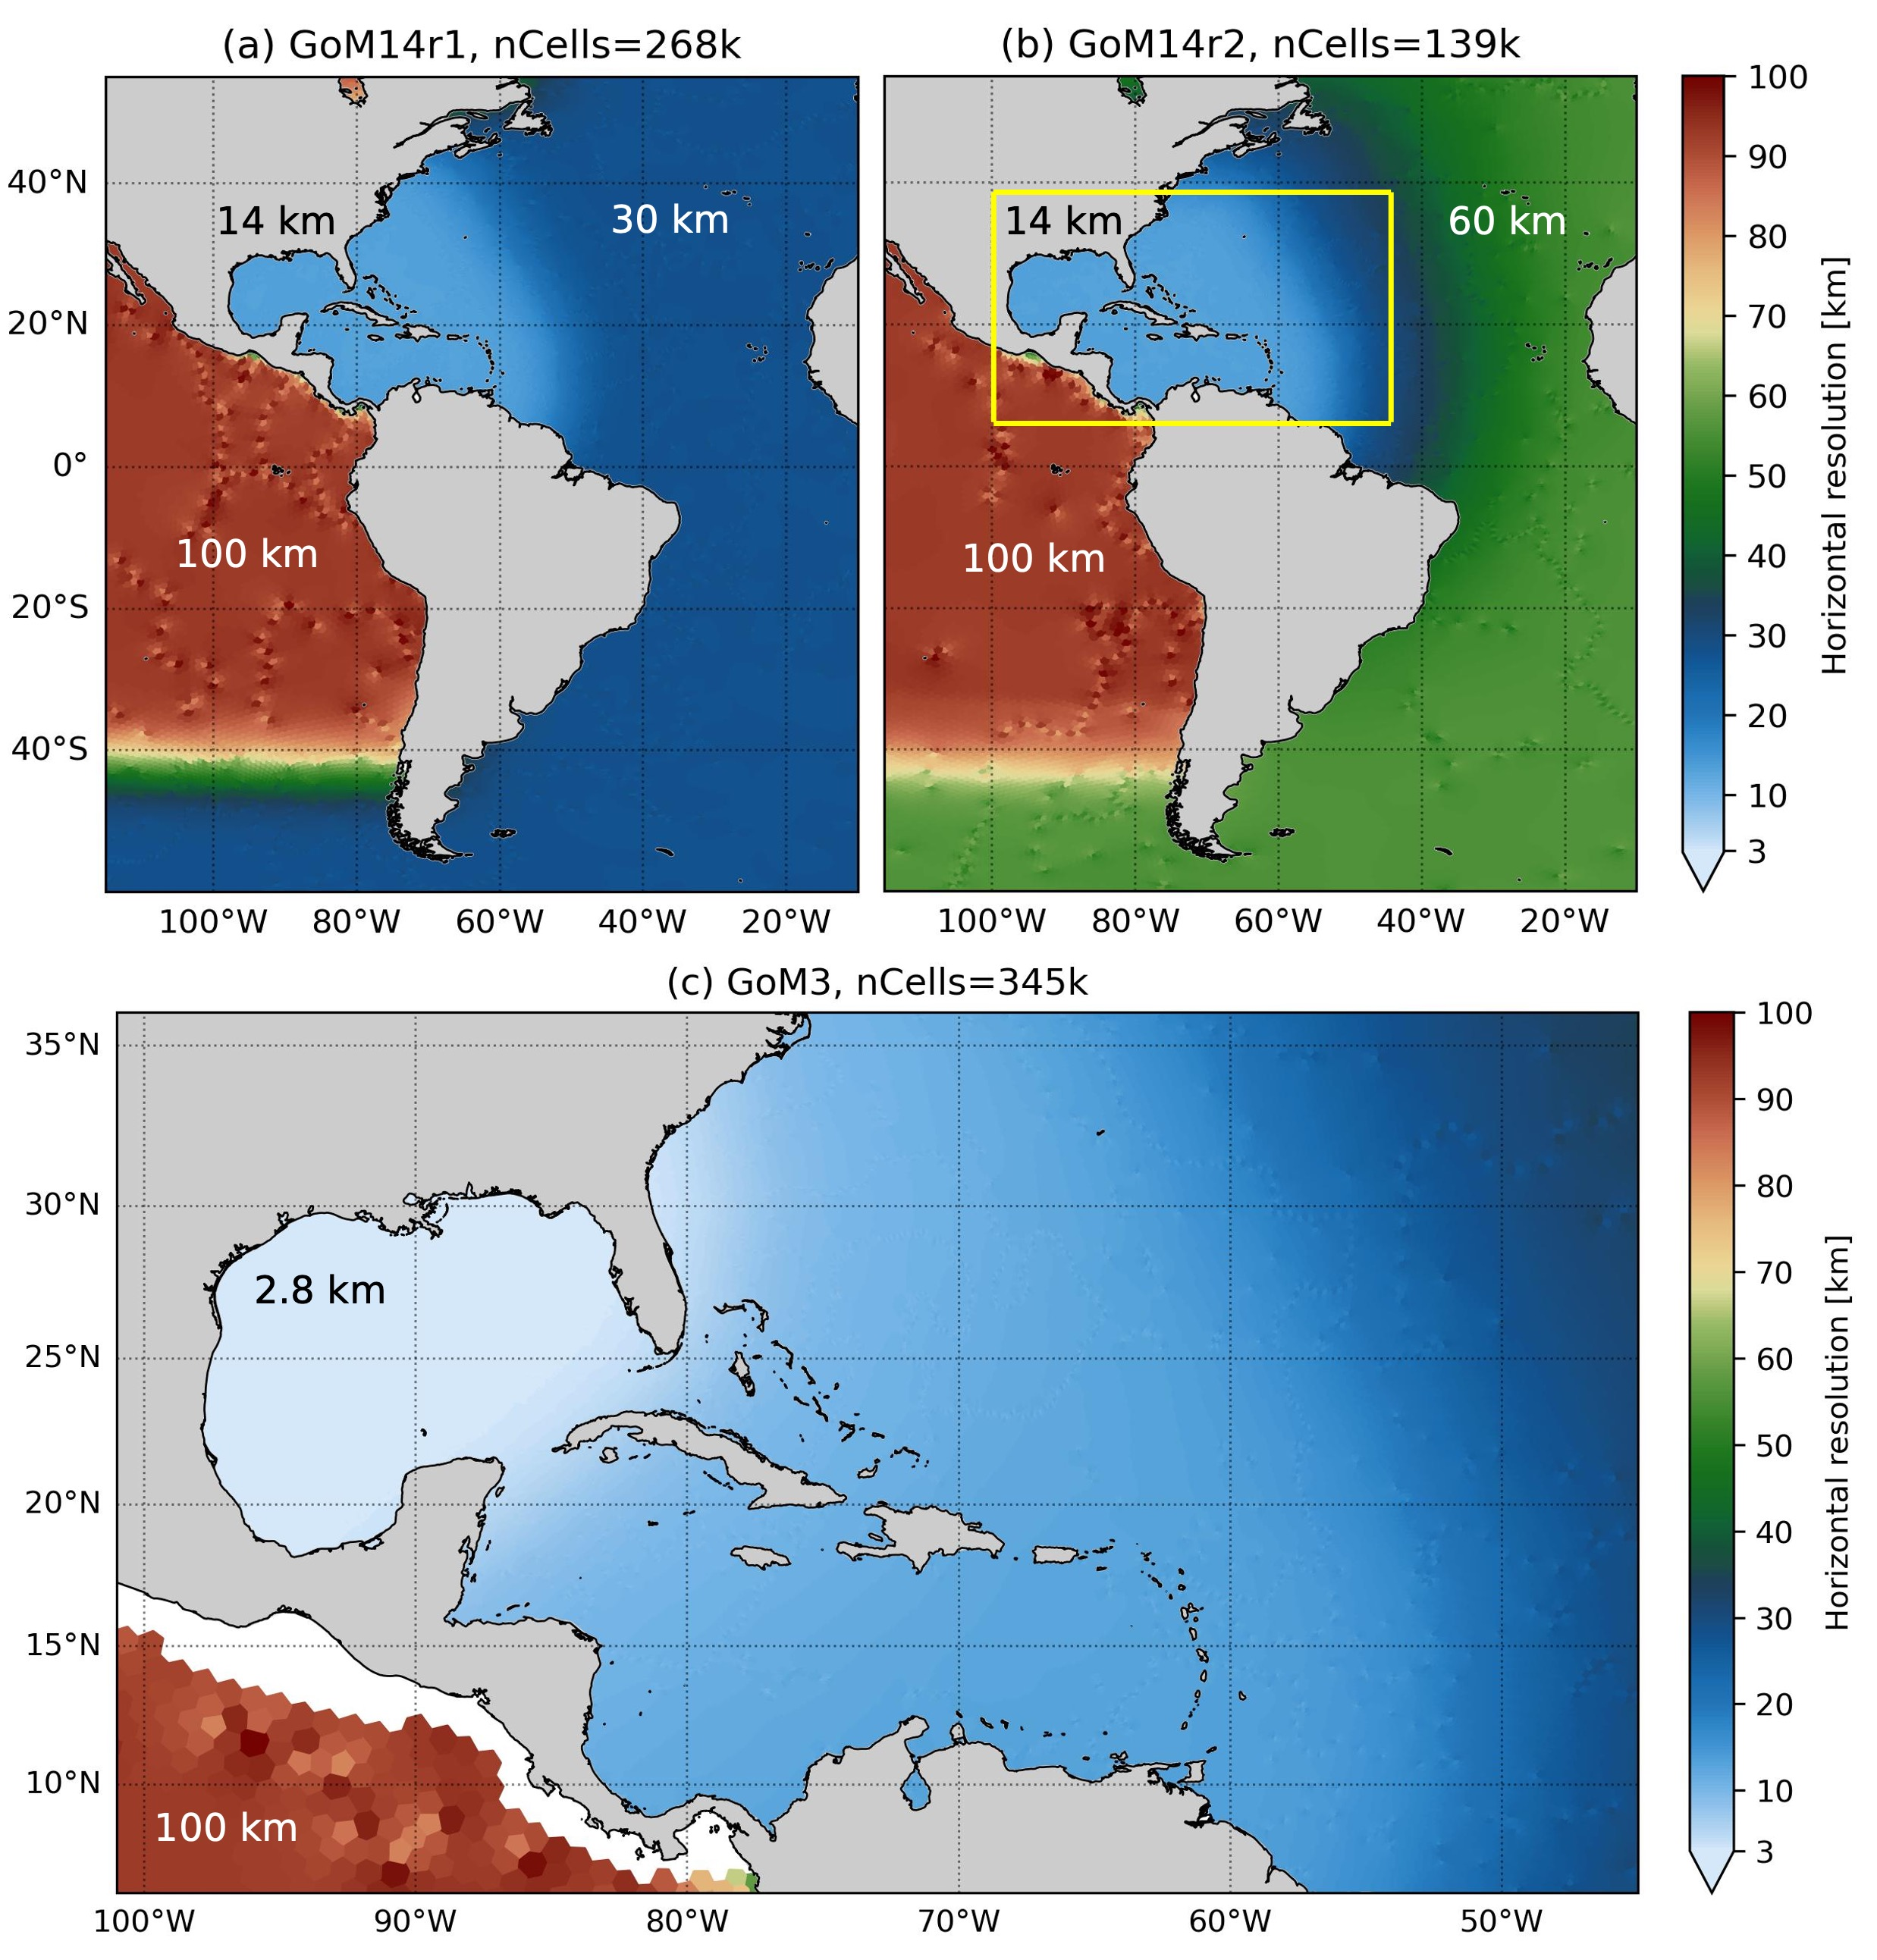
\includegraphics[width = \textwidth]{figures/scgsr/gom_resolutions.jpg}}
    \caption{Horizontal grid cell resolution for GoM14r1 (a), GoM14r2 (b), and GoM3 simulations (c). The broader Pacific and Indian Oceans (not shown) are set to a horizontal resolution of 100 km.}
    \label{fig:mesh_overview}
\end{figure}

First, the TXLA shelf has been the subject of intense observational and modeling efforts due to seasonal occurrences in hypoxia and the 2010 \textit{Deepwater Horizon} oil spill \citep{bianchi2010science,  dukhovskoy2021development, Zhang_2012_forecast}, which allows for an accurate assessment of the fidelity of MPAS-O in representing GoM coastal processes. The MPAS-O simulations developed here are directly compared with the validated ROMS-based TXLA model, which has been run at submesocale eddy-permitting resolution ($\mathcal{O}$(1.5 km)) in early iterations used for hypoxia studies \citep{ruiz2021small, Zhang_2012_numerical}, submesoscale eddy-resolving resolution ($\mathcal{O}$(300 m)) in a two-way nested iteration to aid observational campaigns focused on submesoscale fronts \citep{Qu_2022_NIW, Schlichting23}, and front-refined resolution simulations ($\mathcal{O}$(100 m)) used to understand processes identified from the observations \citep{qu2022rapid}. Second, circulation patterns over the shelf exhibit pronounced seasonal variability, allowing us to assess MPAS-O's representation of submesoscales under variable forcing, a challenging test case. Third, the TXLA shelf features a wind-driven inner shelf circulation inshore of the 50 m isobath, whereas interactions between the plume and loop current (LC) eddies influence the outer shelf circulation \citep{zhang2014wind}. Therefore, the location and gradient of the transition region to a lower grid resolution outside the GoM deserves special consideration so that a realistic loop current is produced.

In the following, we describe the mesh generation process, changes to river forcing, and tuning of key subgrid-scale parameterizations that were shown to have a significant impact on the permitted submesoscales' characteristics. We present preliminary analysis of the GoM3 meshes and compare the representation of surface fronts and the M/A River plume structure with existing TXLA model output. We discuss the strengths and limitations of the current MPAS-O code base that may be used to inform future capability development and regionally refined applications. Finally, we conclude with a discussion of MPAS-O's utility for coastal refined simulations relative to a model nesting approach and discuss future work.

\section{Submesoscale variability in the GoM}
Here we will give a brief overview of the life cycle and seasonal variability of submesoscales over the TXLA shelf and broader GoM to contextualize model results. As reviewed in previous studies \citep{McWilliams_2016, taylor2023submesoscale}, the lateral density (buoyancy) gradient is a key variable that modulates submesoscale generation. Over the TXLA shelf, lateral density gradients are dominated by salinity variations due to freshwater input from the M/A rivers \citep{Hetland_2017}. While, over the broader GoM, density gradients are modulated by both mesoscale eddies shed from the LC and freshwater input from the M/A Rivers \citep{bracco2019mesoscale, liu2021submesoscale}. Submeoscales extract energy from the mixed layer by releasing potential energy stored in the lateral density gradients. The strength of these submesoscales is then closely related to the mixed layer depth because a deeper mixed layer allows for more potential energy to be released \citep{boccaletti2007mixed, fox2008parameterization}. In the open ocean, submesoscales tend to follow a seasonal cycle where they are stronger in winter due to a deeper mixed layer and weaker in summer \footnote{The mixed layer depth is shallower on average in summer due to increased radiative heating.} \citep{callies2015seasonality}. 

In the TXLA shelf region, submesoscales are primarily generated by mixed layer instabilities and surface frontogenesis, or the sharpening of horizontal density gradients \citep{hoskins1982mathematical, mcwilliams2021oceanic}. Frontogenesis is thought to be a primary generation mechanism in the Louisiana Bight west of Southwest Pass and M. River jet east of Bird's Foot \citep{Barkan_2017, wang2021structure}, whereas baroclinic mixed layer instabilities dominate submesoscale generation west of Atchafalaya Bay \citep{Hetland_2017, Schlichting23}. During summer months (JJA), M/A river discharge relaxes relative to spring and a weakly up-coast diurnal land-sea breeze causes freshwater to pool over the shelf, which creates baroclinic instabilities that develop into a rich submesoscale eddy field \citep{Hetland_2017, Kobashi_2020, Schlichting23}. During nonsummer months, downwelling-favorable winds, higher relative river discharge, and cold front passages reduce the stratification created during summer and produce a bottom-advected plume that suppresses eddy formation \citep{hetland2012integrated, zhang2014wind}.

In the broader GoM, \citet{barkan2017submesoscalepart2} showed river discharge can enhance or suppress submesoscales forming near LC eddies over the northern continental shelves. River discharge can energize LC eddy (LCE) fronts by providing a source of brackish water, or suppress them by increasing near-surface stratification. River discharge rates are generally lower during winter (DJF), so submesoscales are generally thought to be more prevalent in the winter than summer. In addition, "submesoscale soup" forms year-round in the eastern GoM and over the Florida shelf, consisting of chaotic fronts, filaments, and eddies \citep{Barkan_2017, liu2021submesoscale}. Given the seasonal differences and the strong freshwater river plume control in both regions, our analysis of the MPAS-O simulations will mostly focus on the surface structure of the M/A river plume and basic estimates of seasonal variability over the TXLA shelf and broader GoM. 

\section{Model setup} \label{sec:coupled_setup}
\subsection{TXLA ROMS model}
The iterations of the TXLA ROMS model are described in previous studies \citep{Kobashi_2020, qu2022rapid, Schlichting23}. Here, we review the dynamical core, discretization methods, subgrid-scale parameterizations, and model forcing so they can be compared with the coupled MPAS-O simulations. The simulations here use the Coupled Ocean-Atmosphere-Wave-Sediment Transport Model \citep{Warner_2010} version of ROMS.

ROMS uses the incompressible, hydrostatic and Boussinesq approximations to solve the primitive equations on a structured, curvilinear Arakawa C-grid \citep{Arakawa_1977, shchepetkin2005regional}. ROMS uses a split explicit time stepping scheme with several numerical methods available for the stepping the baroclinic and barotropic modes. In the simulations presented here, the baroclinic mode is stepped with a third order Adams Bashforth scheme and the barotropic mode is stepped with a third order Adams Moulton-Leapfrog scheme. The tracers are stepped with a trapezoidal leapfrog scheme. Momentum advection is computed using a third order upwind scheme and tracer advection is computed with the multidimensional positive definite advection transport algorithm \citep{Smolarkiewicz_1998}. The simulations here use an 80 s baroclinic timestep and a two s barotropic timestep. 

The TXLA model domain in shown in Fig. 1 of \cite{Schlichting23}, with horizontal resolution varying from 0.6 km close to the coast to 3.7 km near the outer continental slopes. Inshore of 100 m depth, the model resolution is approximately 1.5 km for the analysis region in this paper, which is the location of the child grid used in a nested application \citep{Schlichting23}. The model uses terrain following vertical coordinates with 30 vertical layers stretched near the surface to better resolve the surface boundary layer. The mean vertical resolution in the top one m of the water column (where the M/A plume is most prominent) is approximately 38 cm in the region of interest. The minimum water depth $h_{min}$ is 5 m. 

The TXLA model uses the $k-\omega$ vertical mixing scheme, a two equation model configured as part of the Generic Length Scale library \citep{umlauf2003extending, Warner_2005}. The model uses a geopotential aligned horizontal mixing scheme with constant values scaled to the grid size \citep[see Section 3.2 of ][]{Schlichting23}. The open boundary is forced by Gulf of Mexico HYCOM as described in \citep{Zhang_2012_forecast}. ERA-interim datasets are used to provide surface fluxes \citep{Dee_2011} and river forcing is provided daily by USGS streamflow data for nine regional rivers. Although model snapshots are saved hourly, they are subsampled each day so sampling frequency matches MPAS-O output. Further ROMS documentation is available at \url{https://github.com/kshedstrom/roms_manual/blob/master/roms_manual.pdf}.

\subsection{The model for prediction across scales-ocean (MPAS-O)}
MPAS-O solves a mimetic finite volume discretization of the primitive equations, which makes use of the incompressible, hydrostatic, and Boussinesq approximations to solve prognostic equations for momentum, thickness (volume), and tracers. A key difference relative to ROMS is that MPAS-O solves a vector invariant form of the momentum equations presented in vorticity-kinetic energy form such that momentum advection is expressed as the sum of the gradient of the kinetic energy and the vector product of velocity and vorticity. This approach is required to guarantee the consistent and compatible evolution of mass, velocity, and potential vorticity for arbitrarily structured Arakawa C-grids \citep{Arakawa_1977, ringler2010unified}. The simulations presented here used a second order Adams-Bashforth split explicit time stepping method. Tracer advection is computed with a monotonic, third order flux-corrected transport scheme described in \cite{skamarock2011conservative}. 

Mesh generation is performed using the JIGSAW library \citep{engwirda2017jigsaw}. As \cite{hoch2020mpas} summarizes, JIGSAW incrementally creates an unstructured mesh by first creating a conforming Voronoi/Delaunay tessellation, which is optimized using Optimal Delaunay Tessellation techniques. As a result, the final mesh can consist of triangular and polygonal cells that guarantee a locally orthogonal C-grid staggering that satisfies the requirements detailed in \cite{ringler2010unified}. The simulations presented here use a geopotential-aligned $z^*$ vertical coordinate that oscillates with the sea surface height, designed within an Arbitrary Lagrangian-Eulerian framework \citep{Petersen_2015, griffies2020primer}. 

The vertical mixing scheme is the K-Profile Parameterization \citep[KPP, ][]{large1994oceanic, van2018kpp} configured as part of the CVMix library (\url{https://cvmix.github.io/}). The Gent-McWilliams (GM) thickness advection scheme \citep{gent1990isopycnal} is used to parameterize horizontal transport by mesoscale eddies. The GM scheme is applied to grid cells larger than 30 km and linearly tapered to zero by 20 km. GM is used in conjunction with an isoneutral-aligned diffusion tensor described by \citep{redi1982oceanic} that is tapered similarly to GM. Coefficients used for the GM ($\kappa_{GM}$) and Redi ($\kappa_{redi}$) schemes for all GoM simulations are shown in Tab. \ref{tab:mpaso_sims}. Harmonic ($\nu_2$) and biharmonic ($\nu_4$) lateral viscosity are applied to the momentum equations and scaled to the grid size as 
\begin{equation}
    \nu_2 = \nabla_0^4 \, [\textrm{m}^2 \textrm{s}^{-1}] \frac{\Delta x}{30 \, [\textrm{km}]} \, ,
\end{equation}
\begin{equation}
    \nu_4 = \nabla_0^4 \, [\textrm{m}^4 \textrm{s}^{-2}] \left(\frac{\Delta x}{30 \, [\textrm{km}]}\right)^3 \, ,  
\end{equation}
where $\nabla_0^2$ and $\nabla_0^4$ are the background coefficients for $\nu_2$ and $\nu_4$, respectively, and $\Delta x$ is the horizontal cell width. No explicit horizontal diffusion is applied to the tracers. 

\begin{table}[t] 
\caption{Key parameters used in the GoM refined simulations as defined in text. $^*$ The mean value of $\nabla_0^4$ used in the GoM3r1 simulation is 2.35e10 [m$^4$s$^{-2}$]. $^+$ The mean value of $\nabla_0^4$ used in the GoM3r2 simulation is 3.25e10 [m$^4$s$^{-2}$].} \label{tab:mpaso_sims}
\begin{center}
\begin{tabular}{ccccc}
\hline
Variable & GoM14r1 & GoM14r2 & GoM3r1 & GoM3r2 \\
nCells [$10^5$] & 2.68 & 1.39 & 3.45 & 3.45 \\
$h_{min}$ [m] & 20 & 20 & 20 & 10 \\
$z_{lay}$ [m] & 64 & 64 & 64 & 128 \\
$z_{min}$ [m] & 10 & 10 & 10 & 2 \\
DT [min:s] & 10:00 & 10:00 & 02:30 & 02:30 \\
BTR\_DT [min:s] & 00:15 & 00:15 & 00:07.5 & 00.07.5 \\
$\nabla_2^0$ [m$^2$s$^{-1}$] & 462 & 462 & 66.7 & 66.7 \\
$\nabla_4^0$ 10$^{10}$[m$^4$s$^{-2}$] & 1.2 & 1.2 & 2.0-3.5$^*$ & 2.0-4.5$^+$ \\
$\kappa_{GM}$ [m$^2$s$^{-1}$] & 600 & 600 & 300 & 300 \\
$\kappa_{redi}$ [m$^2$s$^{-1}$] & 400 & 400 & 300 & 300 \\
\hline
\end{tabular}
\end{center}
\end{table}

In addition, the simulations are forced by Japanese 55-year reanalysis \citep[JRA-55, ][]{kobayashi2015jra}, which provides surface momentum, heat, and freshwater fluxes and river runoff fluxes at 0.25$^\circ$ resolution every three hours. Tidal forcing is not included because it is still under development for baroclinic applications \citep{barton2022global}. We do not anticipate this to be a significant source of bias for representation of the M/A river plume because tides are weak over the region \citep{DiMarco_1998} and excluded from the TXLA model. The coupled GoM simulations are described in the next section. Further MPAS-O documentation may be found in \cite{petersen2018mpas}.

\subsection{MPAS meshes and coupled simulations}
A primary factor governing our design of the MPAS meshes and coupled simulations is the target simulation length of 11 years (2000-2011), which allows for an estimate of submesoscale variability in the broader GoM and TXLA shelf. We focused on 2000-2010 because we have existing TXLA model output to compare to and there is strong interannual variability among various forcing mechanisms \citep[see Tab. 2 of ][]{forrest2011multivariable}. We configured the GoM simulations as an E3SM ``G case" such that MPAS-O is coupled with an active version of MPAS Sea Ice \citep{petersen2019evaluation, turner2022mpas}, while all other components are driven by data. The outer TXLA shelf circulation is modulated by interactions with LCEs, which are shed stochastically from the LC in roughly three to 17 month intervals \citep{oey2005loop}. High fidelity representation of the LC requires realistic representation of the Atlantic Meridional Overturning Circulation (AMOC). As reviewed by \cite{richardson2005caribbean}, the LC structure is determined by the northward flowing transport via the Caribbean current, which is forced by the North Brazilian and Equatorial currents. These larger-scale currents are affected by the representation of sea ice in the Southern Ocean on subdecadal timescales, thereby necessitating the use of MPAS Sea Ice.

We targeted a 3 km resolution within the GoM, which is slightly higher resolution than models (e.g. GoM-HYCOM, 1/25$^\circ$, \url{https://www.hycom.org/data/goml0pt04}) that typically provide open boundary forcing for shelf-scale regional models. Previous studies that focused on submesoscale variability in the GoM used 1.5 km resolution or higher \citep{barkan2017submesoscalepart2, bracco2019mesoscale, liu2021submesoscale}. While we plan to design a 1.5 km mesh in the future, 3 km was deemed more practical because it allowed us to develop trial simulations more efficiently that were needed to address two aspects of model configuration unrelated to horizontal resolution. The first was the vertical grid; MPAS-O experienced stability issues (discussed later) near the M/A discharge points when run at high vertical resolution ($<$2 m layers). The second was the implementation of the river forcing; in E3SMv2, rivers are spread in an un-physical way for stability reasons. Ideally, river forcing should be treated as point sources as done in regional models like ROMS. However, this was not implemented in E3SM because the model was not initially developed to simulate coastal processes and changing this would require a complete overhaul of the code. Both aspects are discussed further in the following sections. 

The simulations are first spun up in stand alone (just constant atmospheric forcing) for one month with Rayleigh damping to reduce grid scale noise caused by initialization shock and surface gravity waves \cite{petersen2018mpas}. This allows us to reach a target timestep for the coupled simulations that scales proportionally with the smallest cell width (1 min timestep / 1 km cell width). For example, a 150 s baroclinic and 7.5 s barotropic timestep were used in the GoM3 simulations because the smallest grid cell is approximately 2.5 km.

While many initial mesh configurations were tested in the design process (some of which is detailed below), final analysis was performed on two GoM3 simulations with low (10 m layers) - and medium (2 m layers) resolution vertical meshes (GoM3r1, GoM3r2; Tab. \ref{tab:mpaso_sims}). Target vertical resolution was 0.5 m layers to be comparable to the TXLA model. GoM3r1 was analyzed despite the low vertical resolution because the representation of submesoscales in the broader GoM is less dependent on vertical resolution compared to the TXLA shelf and it seldom experienced stability issues. Following preliminary analysis, we restricted run time to two years (2000-2001) following a two year spinup, which allowed for a baseline estimate of seasonal variability in the GoM. A two year spinup is comparable to previous studies focusing on meso- and submesoscale dynamics in the GoM and TXLA shelf \citep{Barkan_2017, Kobashi_2020}. Simulations were run for only two years because they did not produce a submesoscale eddy field over the shelf.  In addition, all ``trial simulations'' used to develop the GoM3 meshes were initialized in 1958 (the first year of JRA forcing).

We ran the GoM3 simulations on 32 nodes with 128 processes per node. High frequency output of key two dimensional variables (e.g. surface active tracers, surface relative vorticity) were saved daily. Three dimensional variables were saved monthly.  

\subsubsection{Horizontal meshes}
The final mesh configurations used in the analysis portion of this study have a relatively course resolution in much of the global ocean, likely too coarse to perform climate length simulations with any accuracy or defend a fully coupled configuration with the other active components of E3SM. This decision was justified for two reasons: 1) the target simulation length is decadal, and the time scale of the Pacific and Indian Ocean currents affecting the larger-scale ocean state within the GoM is much longer, negating a need for an accurate Pacific or Indian ocean state, 2) model tuning is a goal of this project, and higher resolution outside the region of interest increases computational cost, which slows the rate of model tuning experiments. Regarding the latter, the quality of resolved submesoscale features is extremely sensitive to horizontal mixing coefficients and is discussed later. Thus, we used 100 km resolution in the Pacific and Indian Oceans to minimize computational resources spent outside the region of interest. 

We tested two horizontal mesh configurations (Fig. \ref{fig:mesh_overview}) that relax resolution to 30- and 60 km in the broader Atlantic and Southern Oceans, denoted as GoM14r1 and GoM14r2, respectively. Both meshes used 14 km resolution within the GoM, southern Sargasso Sea, and Caribbean Seas. The 14 km mesh was used instead of three km for the GoM because the 14 km mesh allowed us to more efficiently assess the larger-scale currents that affect the LC. The transition from high to low resolution regions used weighted $\tanh$ functions similar to Eqs. 3-4 of \cite{hoch2020mpas}. The transition from 100-60 km (30 km) used a transition width of 1000 km with no offset from the coast. GoM14r1 (Fig. \ref{fig:mesh_overview} a) used a transition width of 1000 km for the 30- to 14 km regions with a 1000 km offset from the coast. GoM14r2 (Fig. \ref{fig:mesh_overview} b) used the same transition width from 100-60 km but includes an additional refinement from 60-30 km that is 3000 km wide and offset 2500 km from the coast. The transition from 30-14 km is the same as GoM14r1. GoM14r1 had nearly twice as many cells (268 thousand) as GoM14r2 (139 thousand), suggesting a 30 km Atlantic and Southern Ocean placed over half the number of cells outside of the region of interest. We provide details of the GoM3 mesh below after analysis of the GoM14 simulations. 

A two year simulation length is insufficient to properly compare biases with the standard and high resolution E3SM test cases \citep{golaz2022doe, caldwell2019doe}. However, we were able to do a quantitative comparison between the GoM14 meshes and get a sense of scale of their differences, especially in the Atlantic Ocean, and a preliminary estimates of model biases. 

We compared GoM14r1 and GoM14r2 using MPAS-Analysis (\url{https://mpas-dev.github.io/MPAS-Analysis/stable/index.html}), a post processing package designed for analysis of coupled E3SM simulations. We present outputs of several analysis tasks: 1) the time- and zonally-averaged barotropic Atlantic MOC streamfunction $\psi$ (Fig. \ref{fig:moc}), 2) time- and zonally-averaged global meridional heat transport (MHT, Fig. \ref{fig:mht}), and 3) time series of inflowing volume transport through the Antilles Archipelago (Fig. \ref{fig:antilles}). The MOC streamfunction was used to qualitatively examine the vertical structure of the meridional volume transport in the Atlantic Ocean. The MHT was directly compared to observations \citep{trenberth2001estimates} and provides an example of tracer transport bias resulting from the low resolution regions. The Antilles inflow may be compared directly against observations and provides larger-scale forcing for the LC. The metrics discussed above were used to determine whether 60 km resolution in the Atlantic is justifiable relative to 30 km resolution. Details of the computations may be found in the MPAS-Analysis documentation. 

\begin{figure}[h]
\centerline{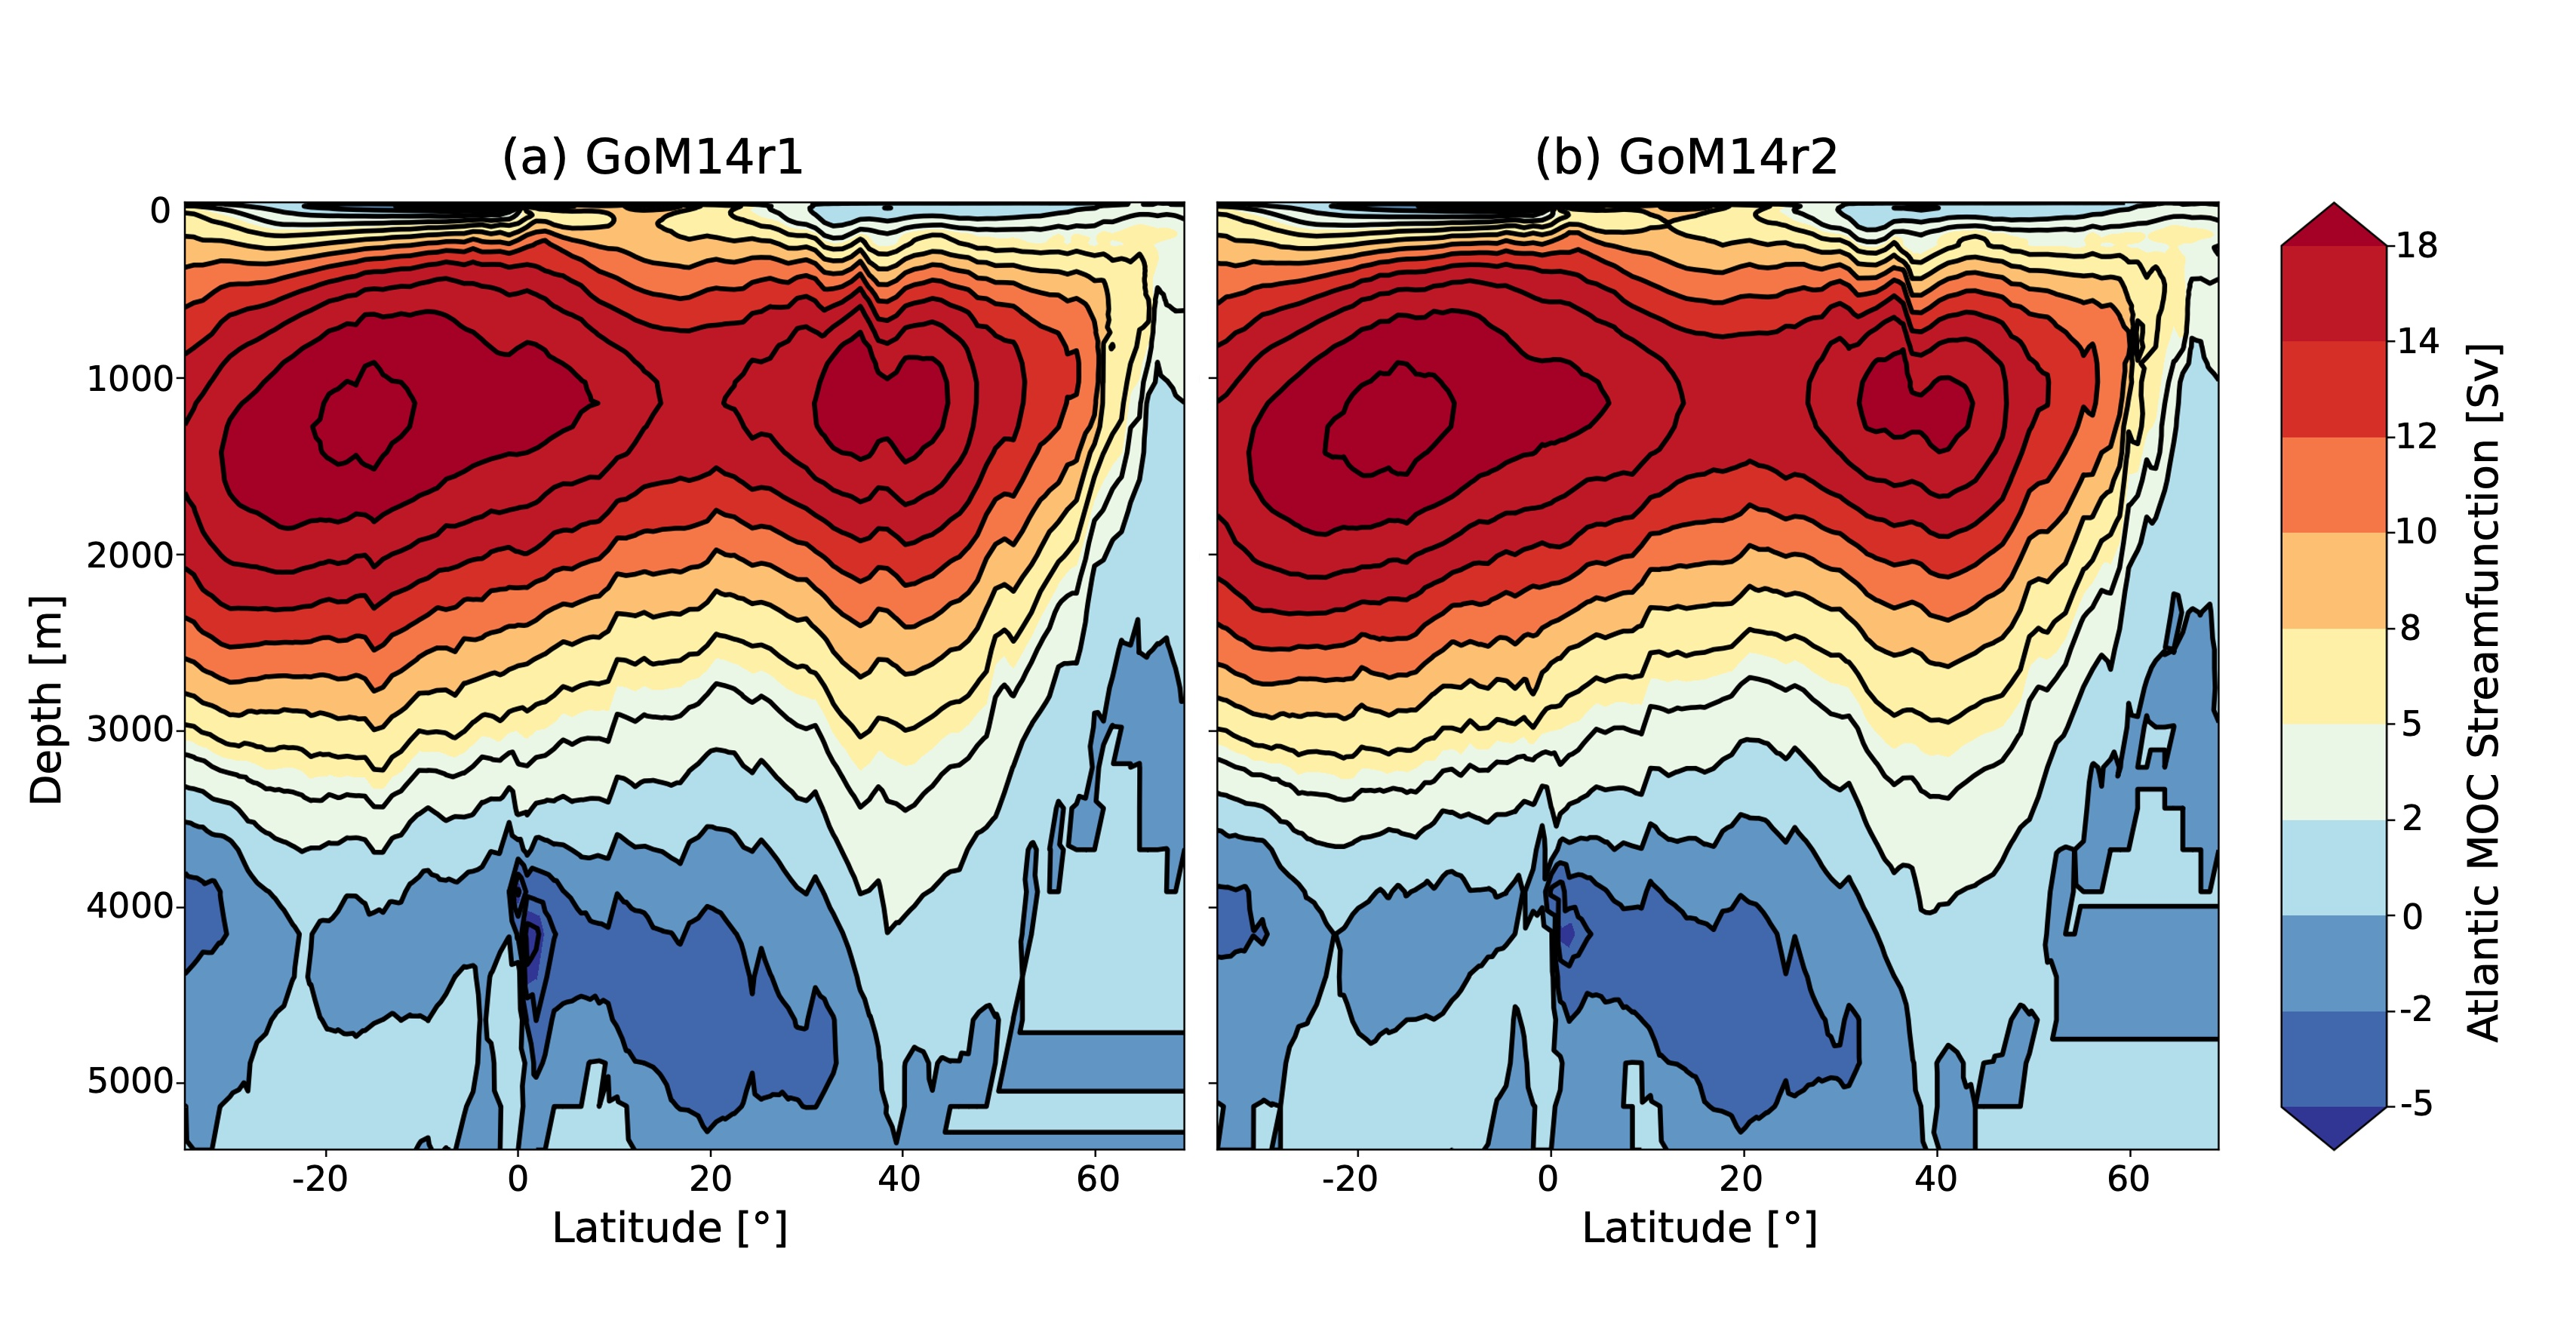
\includegraphics[width=\textwidth]{figures/scgsr/atlantic_moc.jpg}}
    \caption{Zonally-averaged barotropic streamfunction for the Atlantic meridional overturning circulation for GoM14r1 (a) and GoM14r2 (b) integrated over the two year simulation. Contours are overlaid every Sv.}
    \label{fig:moc}
\end{figure}

\begin{figure}[h]
\centerline{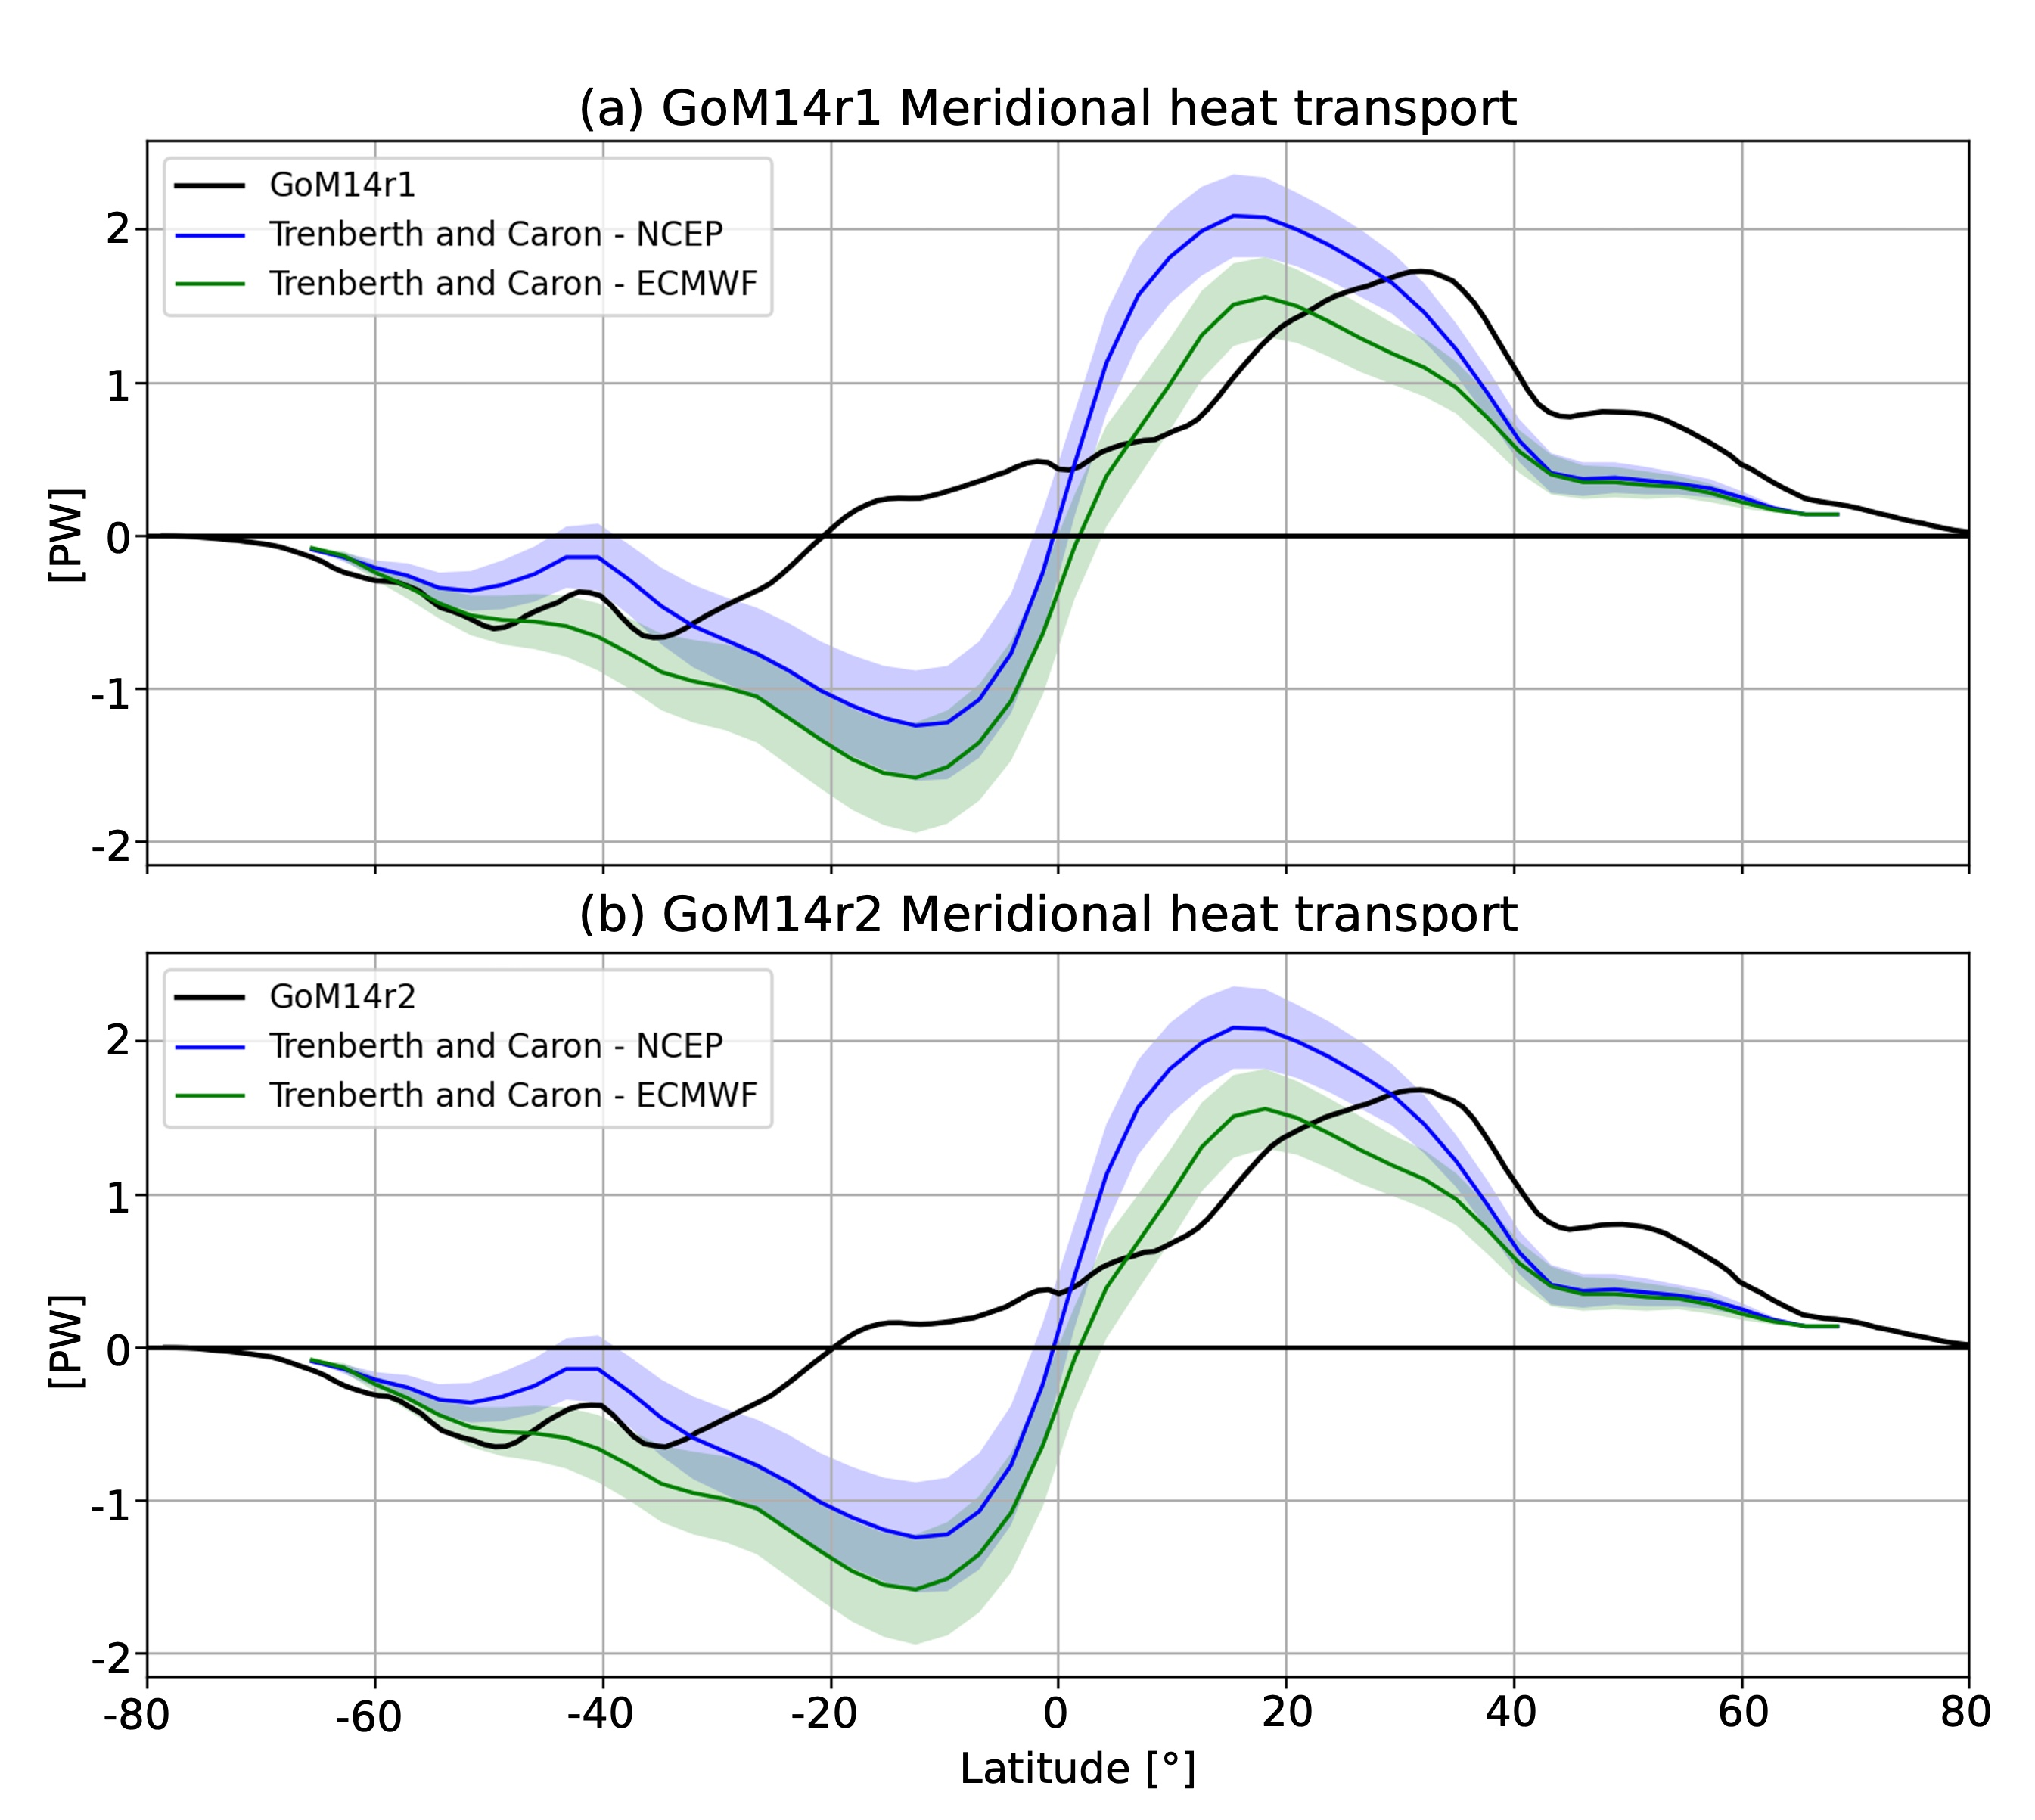
\includegraphics[width=0.9\textwidth]{figures/scgsr/mht_gom14.jpg}}
    \caption{Zonally-averaged MHT for GoM14r1 (a) and GoM14r2 (b) averaged over the two-year simulation relative to observations \citep[see][]{trenberth2001estimates}. The shaded areas represent one standard deviation about the mean of the observations.}
    \label{fig:mht}
\end{figure}

\begin{figure}[h]
\centerline{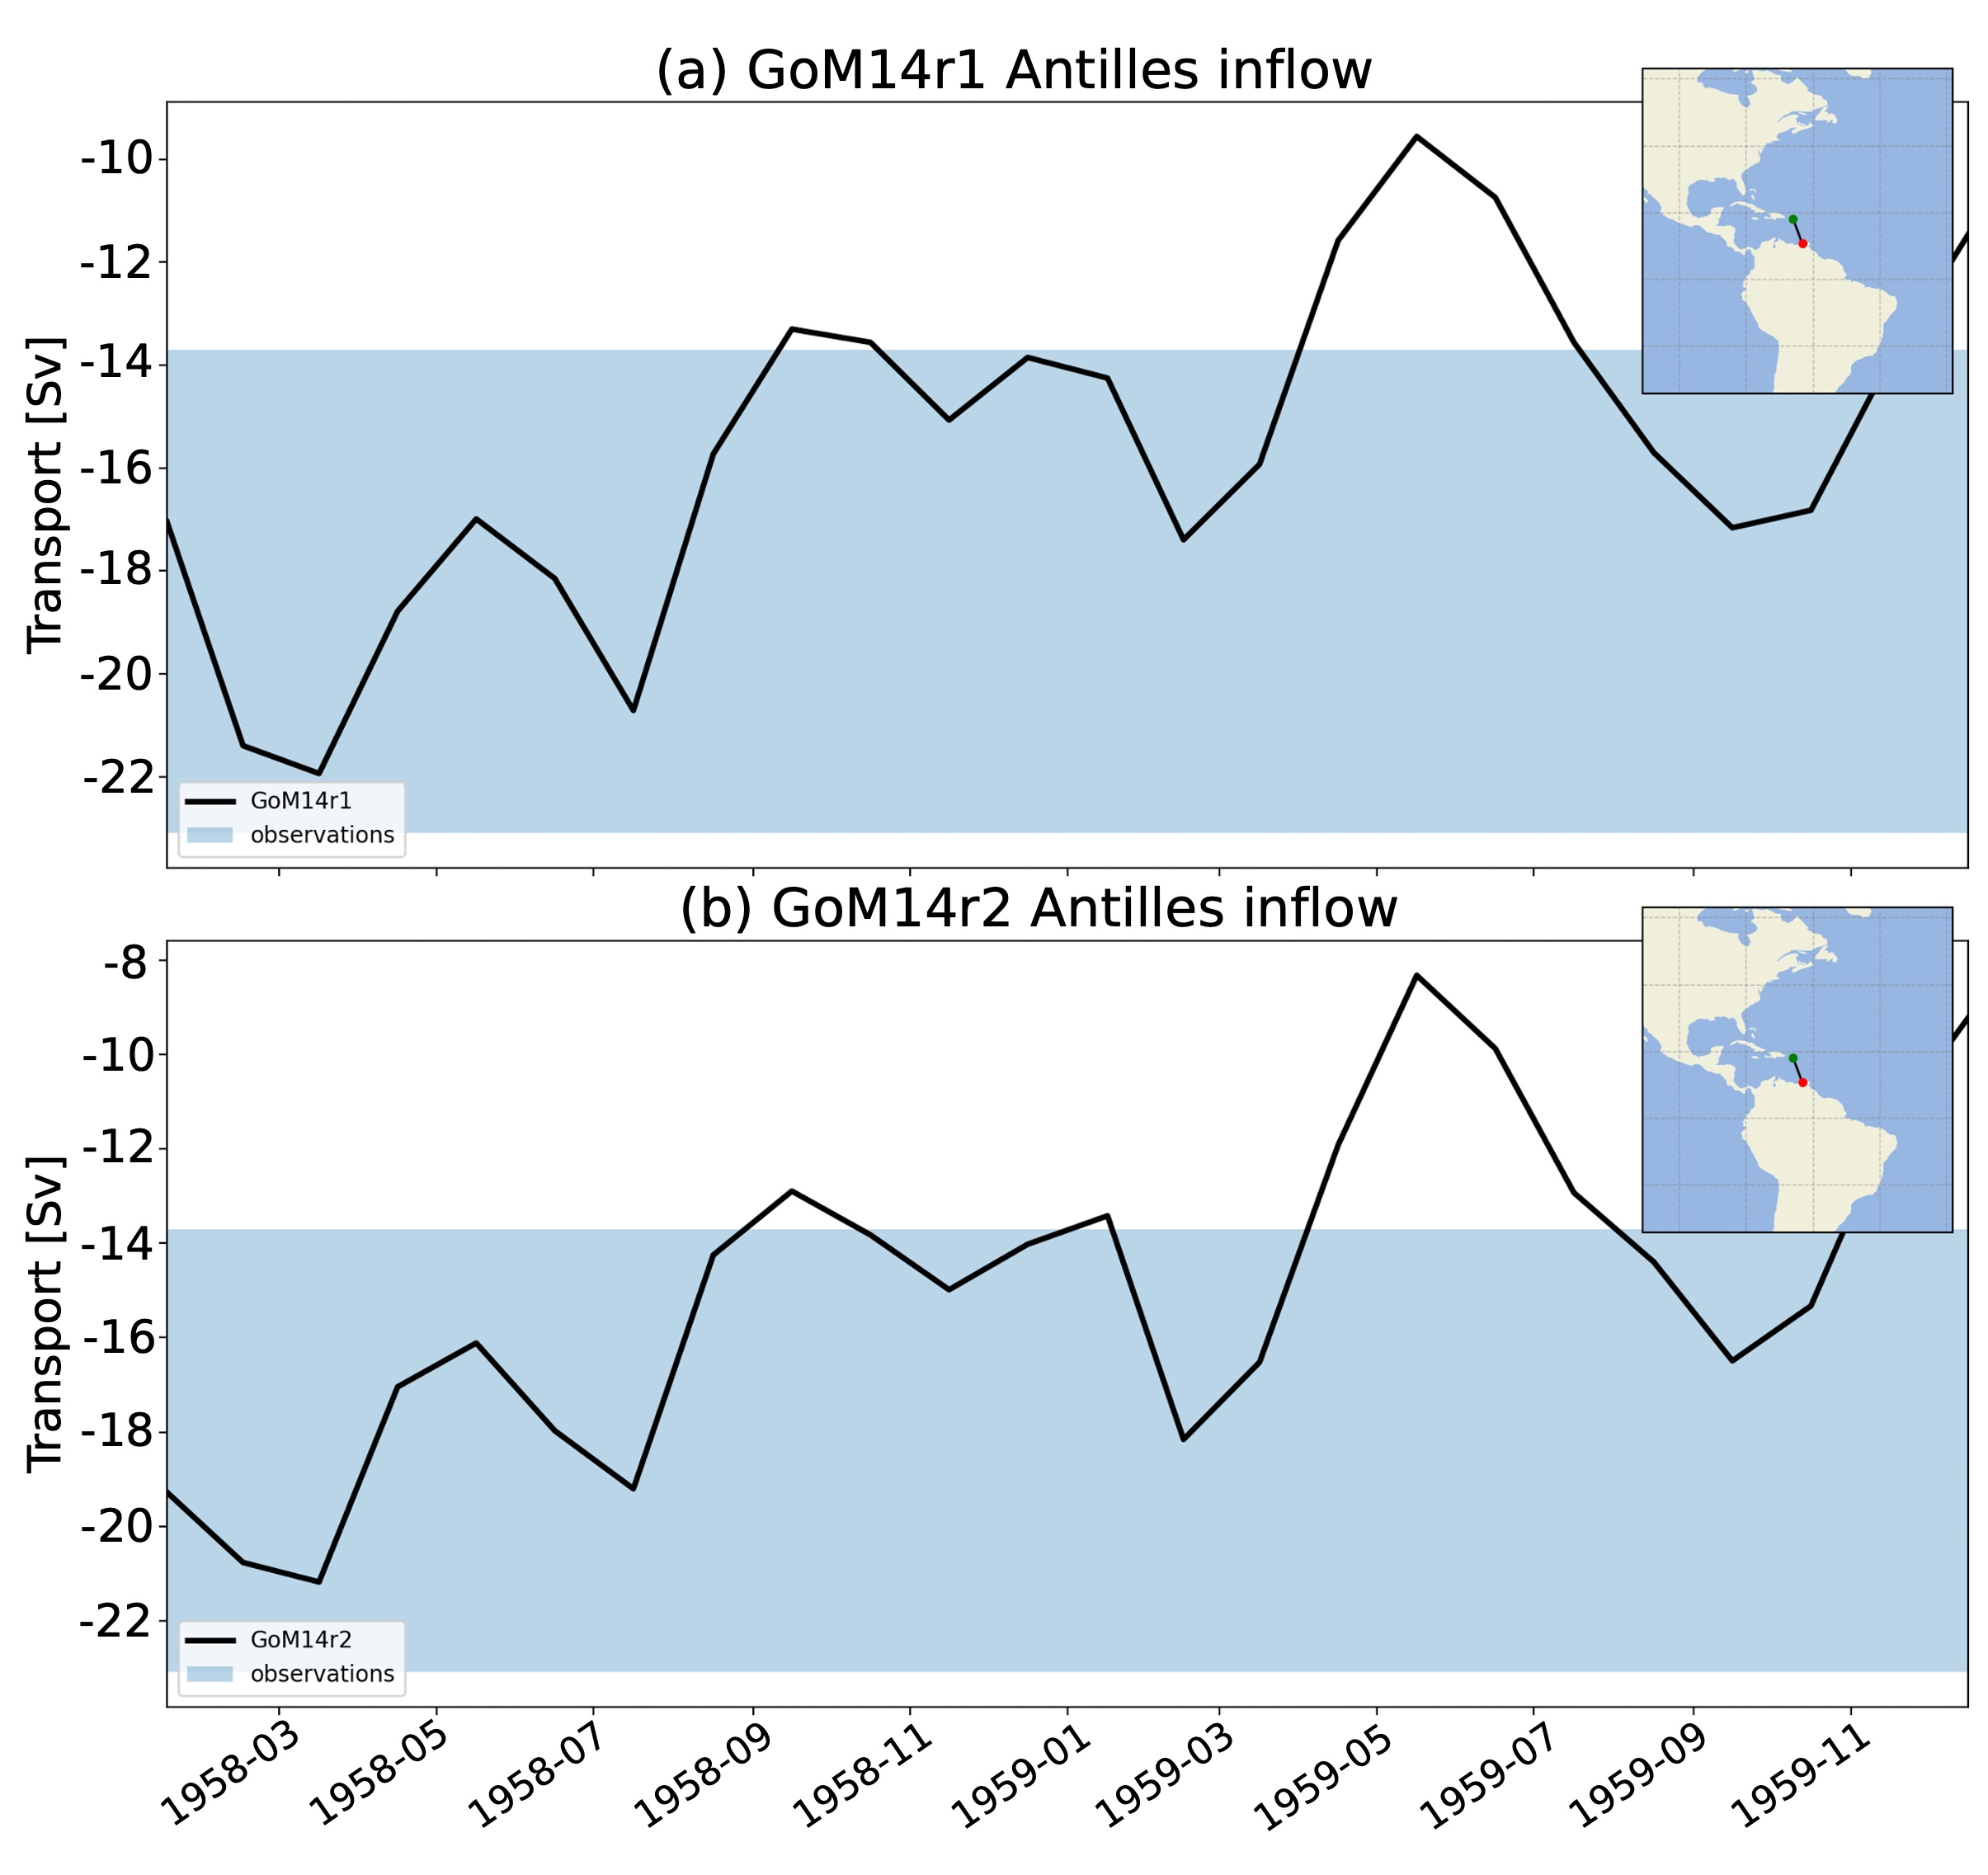
\includegraphics[width=0.8\textwidth]{figures/scgsr/antilles_inflow.jpg}}
    \caption{Time series of inflowing volume transport through the Antilles Archipelago for GoM14r1 (a) and GoM14r2 (b) relative to observations, which are shaded by one standard deviation on either side of the mean value.}
    \label{fig:antilles}
\end{figure}

The MPAS-Analysis results suggest the differences between GoM14r1- and -2 are marginal in the region of interest. The MOC streamfunctions are qualitatively similar south of 40$^\circ$N. North of 40$^\circ$N, GoM14r2 exhibits stronger southward flow ($\psi<0$) below 2000 m depth and weaker northward flow above 2000 m due to coarser resolution. The zonally-averaged MHT transport demonstrates the model biases exceeding 1 PW in the subtropics in both hemispheres and 0.5 PW at midlatitudes of the northern hemisphere. We assume these biases are caused by two factors: 1) Use of JRA-55 for atmospheric forcing instead of coupling with MPAS-Atmosphere, and 2) the 100 km resolution in the Pacific and Indian Oceans. Further investigation these biases is beyond the scope of this study, however, it suggests the GoM3 mesh is likely unsuitable for long term climate simulations. In addition, the Antilles inflow for both meshes are quantitatively similar. However, the transport may be weaker than the observations by up to 4 Sv in the second year of the simulation. This is likely due to the coarse vertical resolution, which poorly resolves much of the continental slopes and islands surrounding the Achilles Archipelago. Thus, we chose to relax the grid resolution to 60 km in the broader Atlantic and Southern Oceans when designing the GoM3 mesh. Complete output of MPAS Analysis for the GoM14 simulations can be found at \url{https://zenodo.org/records/10866134}. 

The GoM3 mesh was designed with a target resolution of 3 km. The transition from 60-30 km is the same as GoM14r2. Two additional refinements are used to achieve target resolution. A transition from 30-9 km over a width of 1800 km that is offset 1200 km from the coast, and a transition from 9- to 3 km over a width of 500 km that is offset 450 km from the coast. The number of cells is 345 thousand, with over half the cells in the region of interest. %While the transition from 60-3 km is small relative to previous meshes, we did not find this to meaningfully impact the representation of submesoscales in the GoM. 

We list several features of JIGSAW that may be useful for future coastal refined meshes. First, high resolution cells appeared off the Pacific coastline of Central America when they were not prescribed. These are present in all GoM refined meshes but were most significant in GoM3, where they caused stability issues. We culled most of these cells because we could not identify an easily actionable solution within JIGSAW, and further investigation was beyond the scope of this study (Fig. \ref{fig:mesh_overview}). Second, the target resolution in each region did not match the prescribed values set by the $tanh$ functions. For example, much of the Pacific Ocean is between 95-100 km resolution and the mean resolution within much of the GoM is 2.8 km, with several dozen cells as small as 2.47 km. Last, there are a significant number of poor quality cells where the resolution deviates significantly from either the target resolution or resolution of neighboring cells. This is most prevalent in the Pacific (Fig. \ref{fig:mesh_overview}).

\subsection{River runoff fluxes}
We modified two aspects of the river runoff fluxes for the GoM3 simulations: the lateral spreading and inflow temperature. In E3SMv2, external mapping files are used to spread river runoff. The magnitude of this spreading, which is applied in the same way for each river, was originally dictated by what is needed to provide stability for the Amazon River outflow. This resulted in all river fluxes being spread hundreds of km offshore (Fig. \ref{fig:spreading} a). Work is being done to modify this spreading such that the distance is proportional to the inflowing runoff fluxes of each river (Fig. \ref{fig:spreading} b), to be released in later versions of E3SM. In this study, we used this newer, more appropriate spreading and applied an additional modification to the M. River, to spread over as small of a region possible that stability constraints allowed. It should also be noted, that E3SM's river-to-ocean mapping algorithm (a nearest neighbor approach) currently releases the M. River out of only the Southwest Pass of Bird's foot. Modifications to split the release of the M. River outflow to its other major outlets will be a focus of future work.

\begin{figure}
\centerline{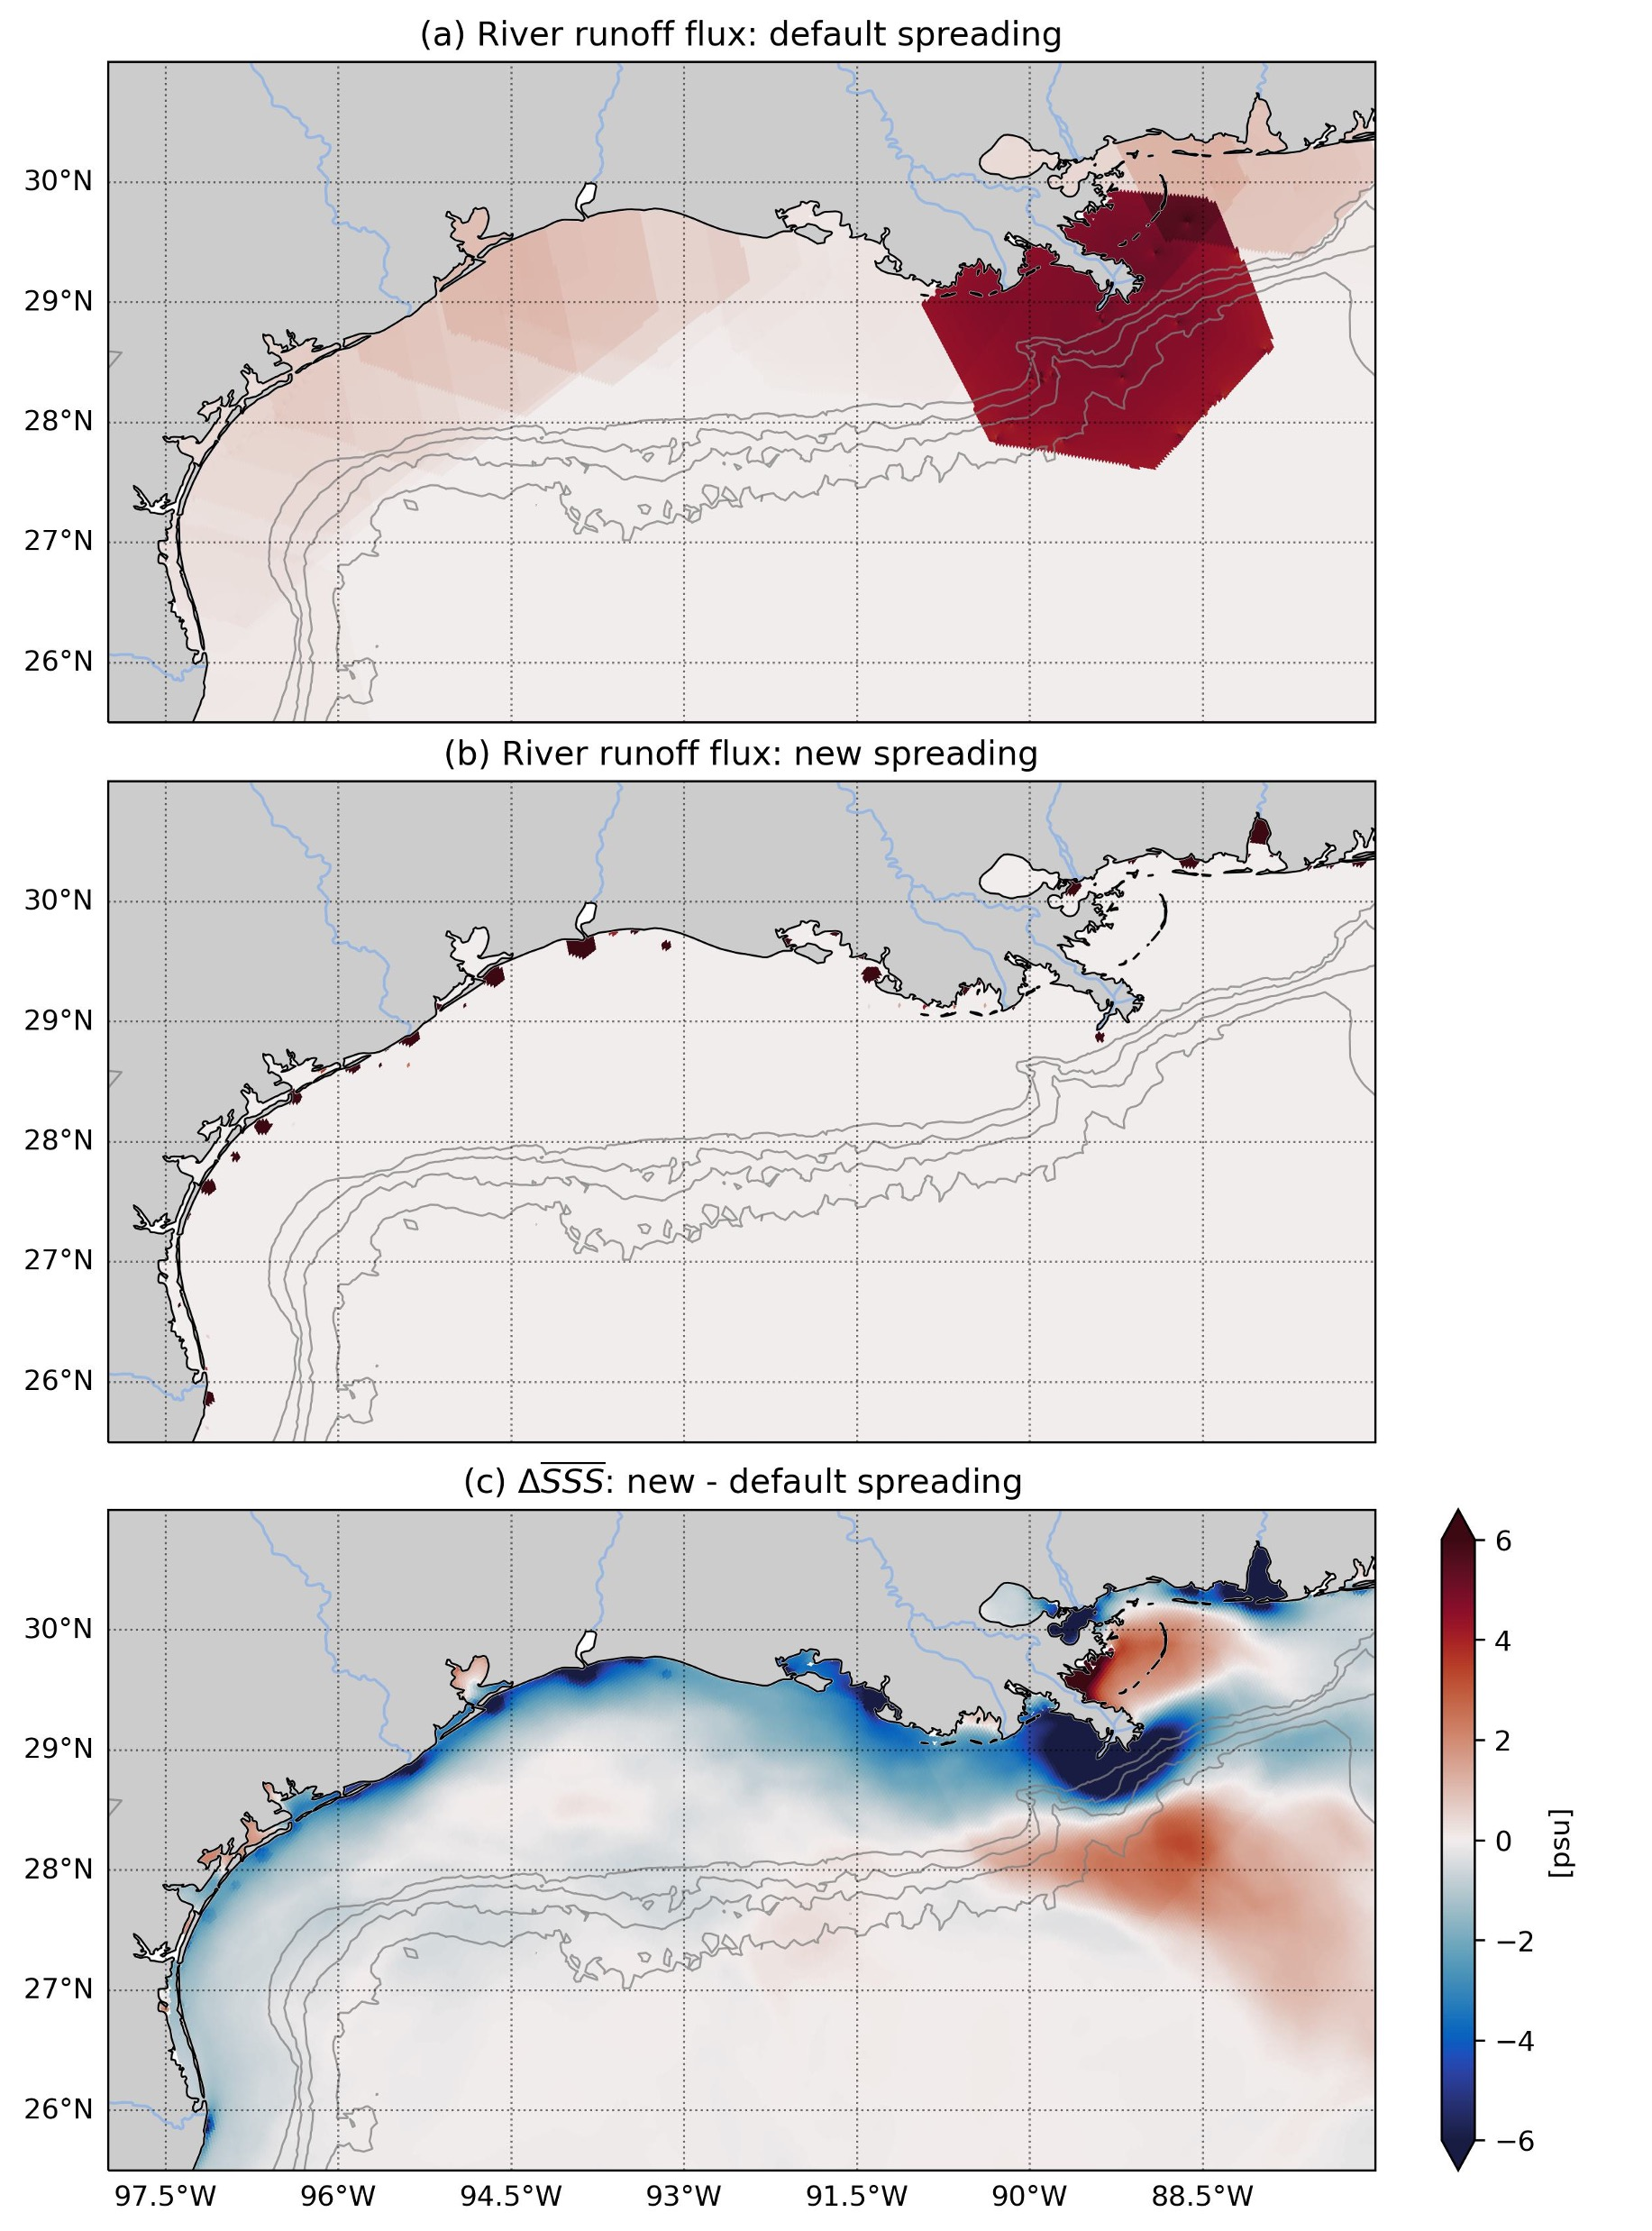
\includegraphics[width=0.95\textwidth]{figures/scgsr/spreading_comp.jpg}}
    \caption{Default river spreading implementation in E3SM v2 (a) and the new implementation developed for the GoM3 simulations (b). (c) Relative difference in the time-averaged sea surface salinity $\Delta \overline{SSS}$ between the new and default spreading for an eight month trial simulation during 1958.}
    \label{fig:spreading}
\end{figure}

The improvement of the new river spreading is shown in Fig. \ref{fig:spreading} (c) with the time-averaged change in sea surface salinity $\Delta SSS$ between the new and default spreading for an eight month trial simulation. The simulation was performed from Jan-Aug, 1958 with 128 vertical layers, 0.2 m layer thickness, and 4 m minimum water depth \footnote{This vertical mesh was later found to be unstable.}. The trial simulation results show the freshwater content over the shelf increases signficantly with the new spreading, with $\Delta \overline{SSS}$ values exceeding six psu near most of the major rivers. The default configuration spreads much of M. River water directly into deep water, which is physically unrealistic and distorted the structure of LC eddies as they are move onto the TXLA shelf (not shown). 

\begin{figure}[t]
\centerline{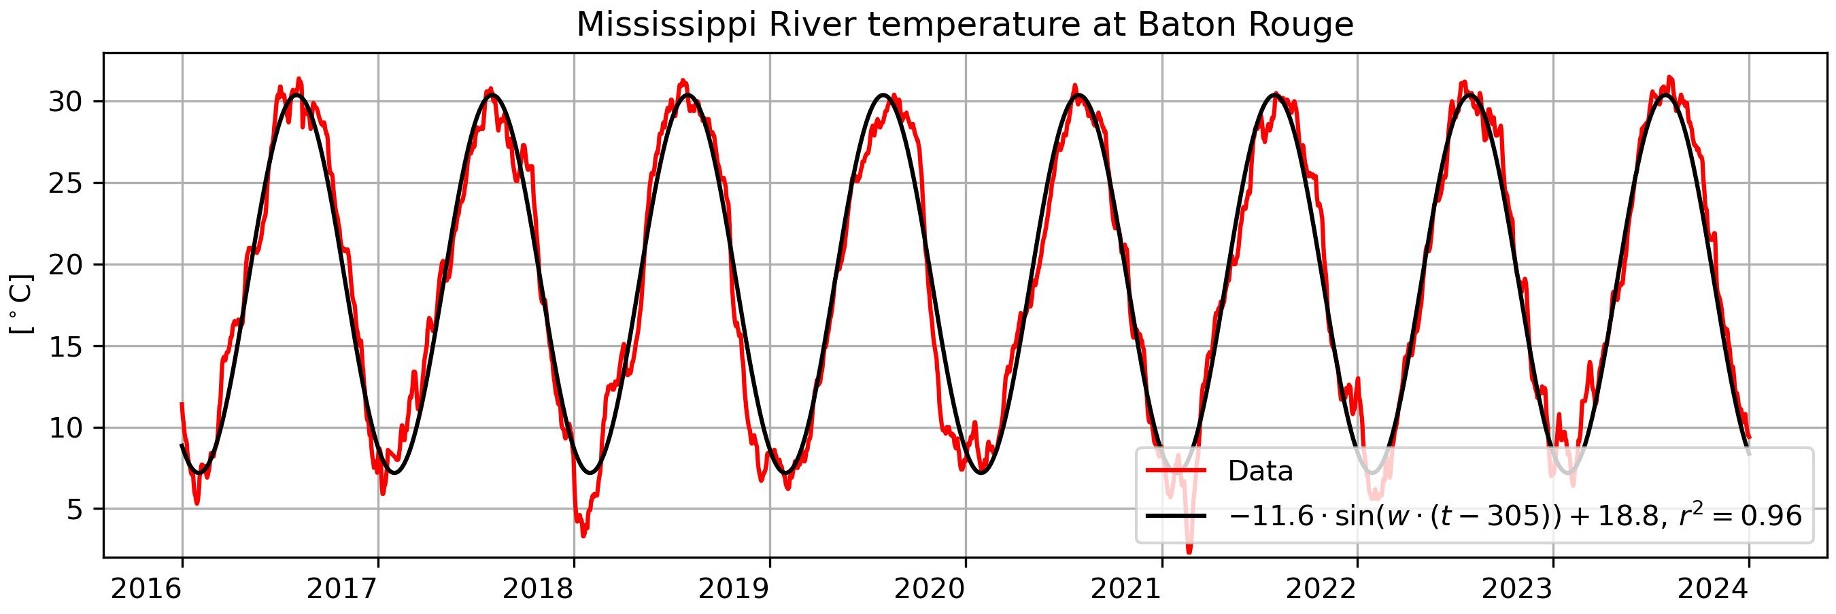
\includegraphics[width=\textwidth]{figures/scgsr/Miss_temp.jpg}}
    \caption{Time series of daily-averaged Mississippi river temperature and fitted sine wave.}
    \label{fig:miss_temp}
\end{figure}

We modified the temperature of the river runoff flux because of stability concerns that arose during vertical resolution experiments. E3SMv2 sets the river temperature equal to the ambient sea surface temperature at the river release location. Trial experiments (not shown) revealed that inflowing water at the spreading points of Southwest Pass was spuriously heated to unrealistic temperatures. To alleviate this issue, we set the inflowing runoff temperatures of all rivers in the GoM to a fitted sine function using eight years of USGS daily-averaged streamflow data at Baton Rouge (\url{https://waterdata.usgs.gov/monitoring-location/07374000}) that covers all years under JRA forcing (1958-present). While setting all inflowing river temperatures equal to the Mississippi is physically unrealistic, there is currently no simple way to apply this modification to only a subset of the rivers in E3SM, this solution guaranteed inflowing river water within the GoM was not spuriously heated, and the time scale of the effects of this solution propagating from regions of the global ocean where this is unrealistic is much longer than the simulations this study analyzes. 

The river temperature function ($\theta_{riv}$) is prescribed daily as
\begin{equation}
    \theta_{riv} = A \sin (\omega [t_{day}-t_{off}] ) + C, 
\end{equation}
where $A$ is the amplitude, $\omega$ is the angular frequency, $t_{day}$ is the model day of year, $t_{off}$ is phase offset, and $C$ is the vertical shift. Values for $A$, $\omega$, $t_{off}$, $C$, and goodness of fit ($r^2$) are shown in Fig. \ref{fig:miss_temp}. 

\subsection{GoM3 vertical meshes}
We developed 18 trial meshes and attempted to make these parameters comparable to the TXLA model. Due to stability issues, we designed a low (GoM3r1) and medium (GoM3r2) resolution vertical mesh with vertical grid parameters $h_{min} = (10,20)$ m, $z_{min} = (10,2)$ m, and $z_{lay} = (64,128)$, respectively. 

GoM3r1 was used for tuning experiments with $\nabla_0^4$ to get a sense of scale for the permitted submesocales in the outer GoM. GoM3r1 uses only three vertical layers where the bottom depth is 20 m and features roughly 10 vertical layers inshore of the 100 m depth. GoM3r2 uses 10 vertical layers at 20 m depth and roughly 50 vertical layers inshore of 100 m depth. While this resolution is insufficient to capture the upper structure of the M/A plume, the middle of the water column is better resolved than the TXLA model.

We determined the stability issues are related to model forcing because all trial meshes ran successfully in stand alone. For example, the highest resolution case used $z_{min} = 0.2$ m and $h_{min} = 1$ m and ran with no Rayleigh damping for one simulated year. Two general scenarios describe the stability issues. First, thin layers (e.g. $z_{min} = 0.2$ m) coupled with shallow bathymetry (e.g $h_{min}=3$ m) caused $z_{min}$ to become negative near the M/A rivers within the first few days of spinup. Second, thin vertical layers ($z_{min} = 0.2$) with unrealistic bathymetry ($h_{min}=10$ m) caused numerical instability at Southwest Pass to form within several months of simulated time, but $z_{min}$ remained positive. The exact cause of the stability issues is still under investigation. 

\subsection{Biharmonic horizontal mixing}
The representation of submesoscales in the GoM is sensitive to the biharmonic mixing coefficient $\nabla_0^4$ because it smooths energy at higher wavenumbers. For example, Fig. \ref{fig:del4} shows snapshots of surface normalized relative vorticity $\zeta f^{-1}$, where $\zeta = \partial_x v - \partial_y u$ and $f$ is the Coriolis parameter, for a simulation using $\nabla_0^4=2.0 \cdot 10^{11}$ [m$^4$s$^{-2}$]) and ($\nabla_0^4=3.33 \cdot 10^{11}$ [m$^4$s$^{-2}$]). The former is the target value selected from six tuning simulations (not shown), where smaller values of $\nabla_0^4$ were found to be unstable, and the latter is the default value used in lower resolution meshes. Higher $\nabla_0^4$ suppresses submesoscales within the GoM, which results in weaker surface fronts, secondary instabilities that form off the LC, and submesocale soup in the eastern GoM. 

\begin{figure} \centerline{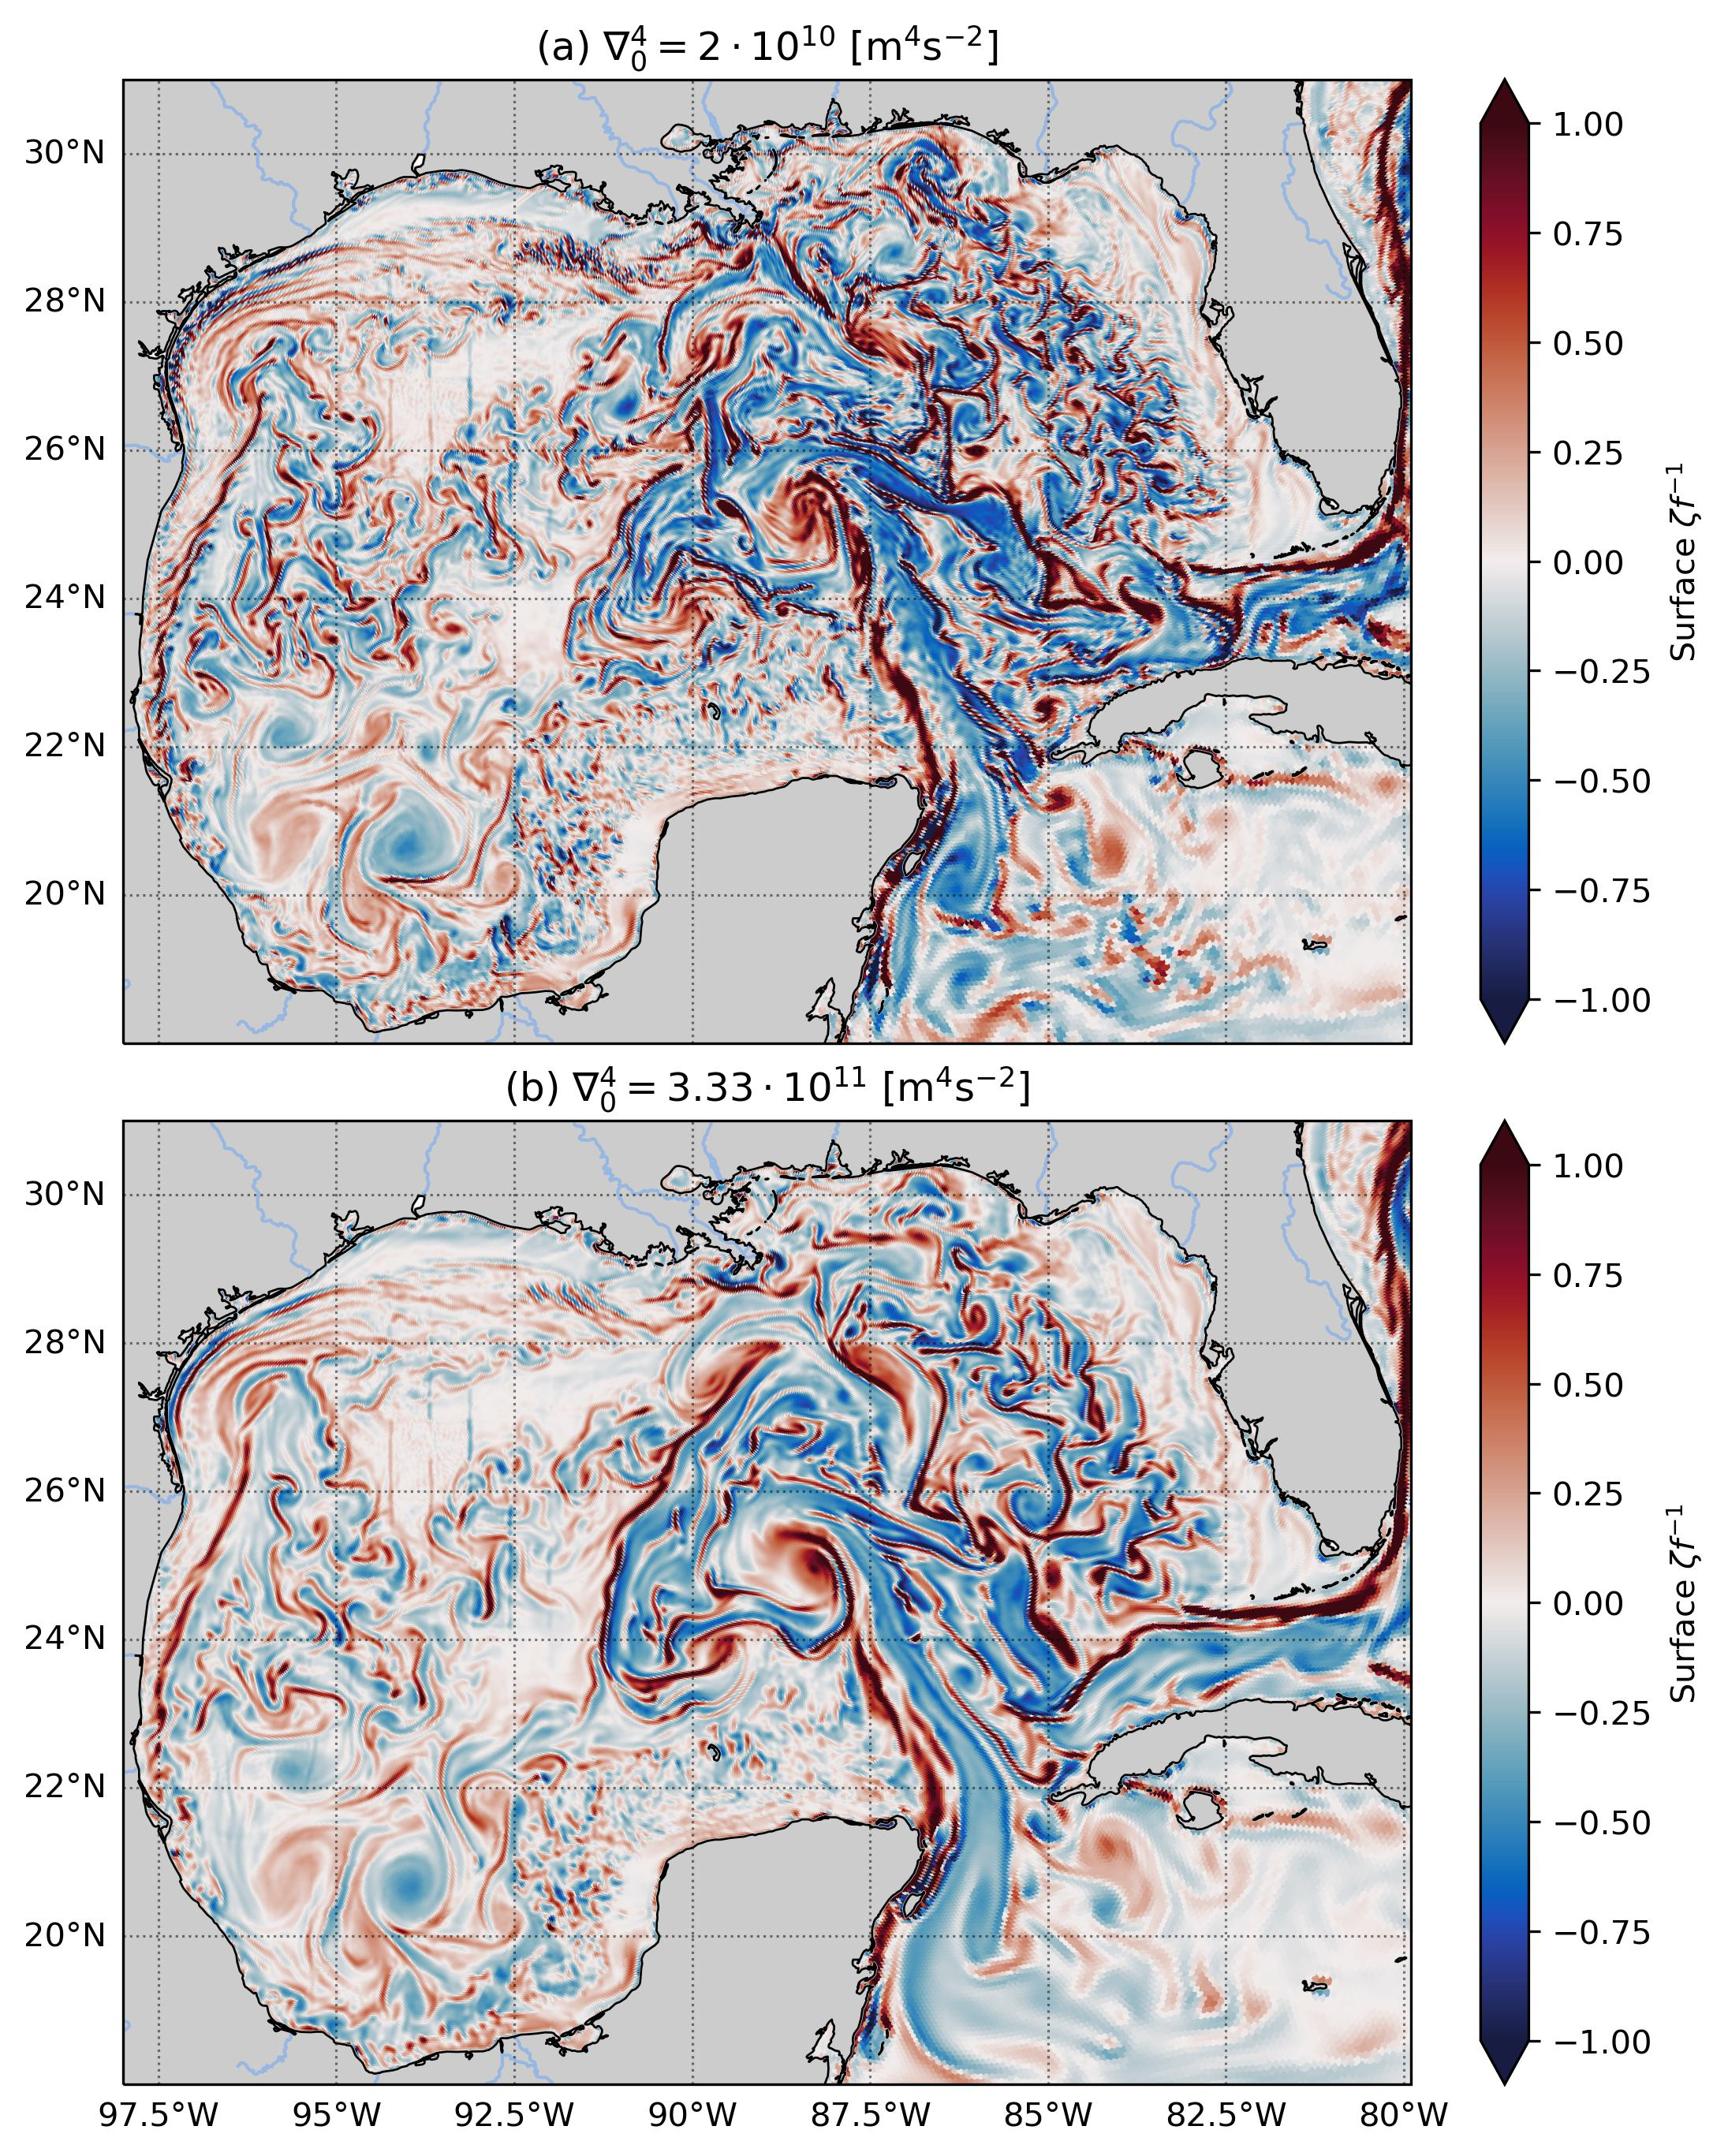
\includegraphics[width=\textwidth]{figures/scgsr/rvort_del4_comp.jpg}}
    \caption{Snapshots of GoM3r1 surface $\zeta f^{-1}$ for different $\nabla_0^4$ values on Feb 22, 1958.}
    \label{fig:del4}
\end{figure}

Periods of higher river discharge (fall and winter) required increases in $\nabla_0^4$ for both GoM3 meshes by over 50\% to maintain stability over the shelf. GoM3r2 required higher $\nabla_0^4$ values relative to GoM3r1 because sharper surface fronts are permitted at higher vertical resolution, especially within the M/A plume. We discuss the implications of this on the representation of surface fronts in the next section. 

\section{Results}
\subsection{Representation of surface vorticity}
Fig. \ref{fig:gom3_rvort_planview} shows snapshots of surface $\zeta f^{-1}$ for GoM3r1 and GoM3r2 during winter and summer. There is an abundance of submesoscale features including fronts, filaments, and eddies found in winter for both simulations. It is encouraging to see the development of secondary instabilities near LC eddies and submesoscale soup forming in the eastern GoM, consistent with previous studies \citep{Barkan_2017, bracco2019mesoscale, liu2021submesoscale}. There are less submesoscales than expected found during summer and frontal eddies seldom form inshore of 100 m depth over the TXLA shelf. Frontal eddies occasionally form over the continental slopes (Fig. \ref{fig:gom3_rvort_planview} c), however they are less organized than eddies found in the TXLA model and the vorticity is about half the magnitude \citep[compare to Fig. 2 of ][]{Schlichting23}. In addition, the submesoscales appear weaker in GoM3r2 despite the higher vertical resolution, which we suspect is due to the higher $\nabla_0^4$ required to maintain stability. 

\begin{figure}[t]
\centerline{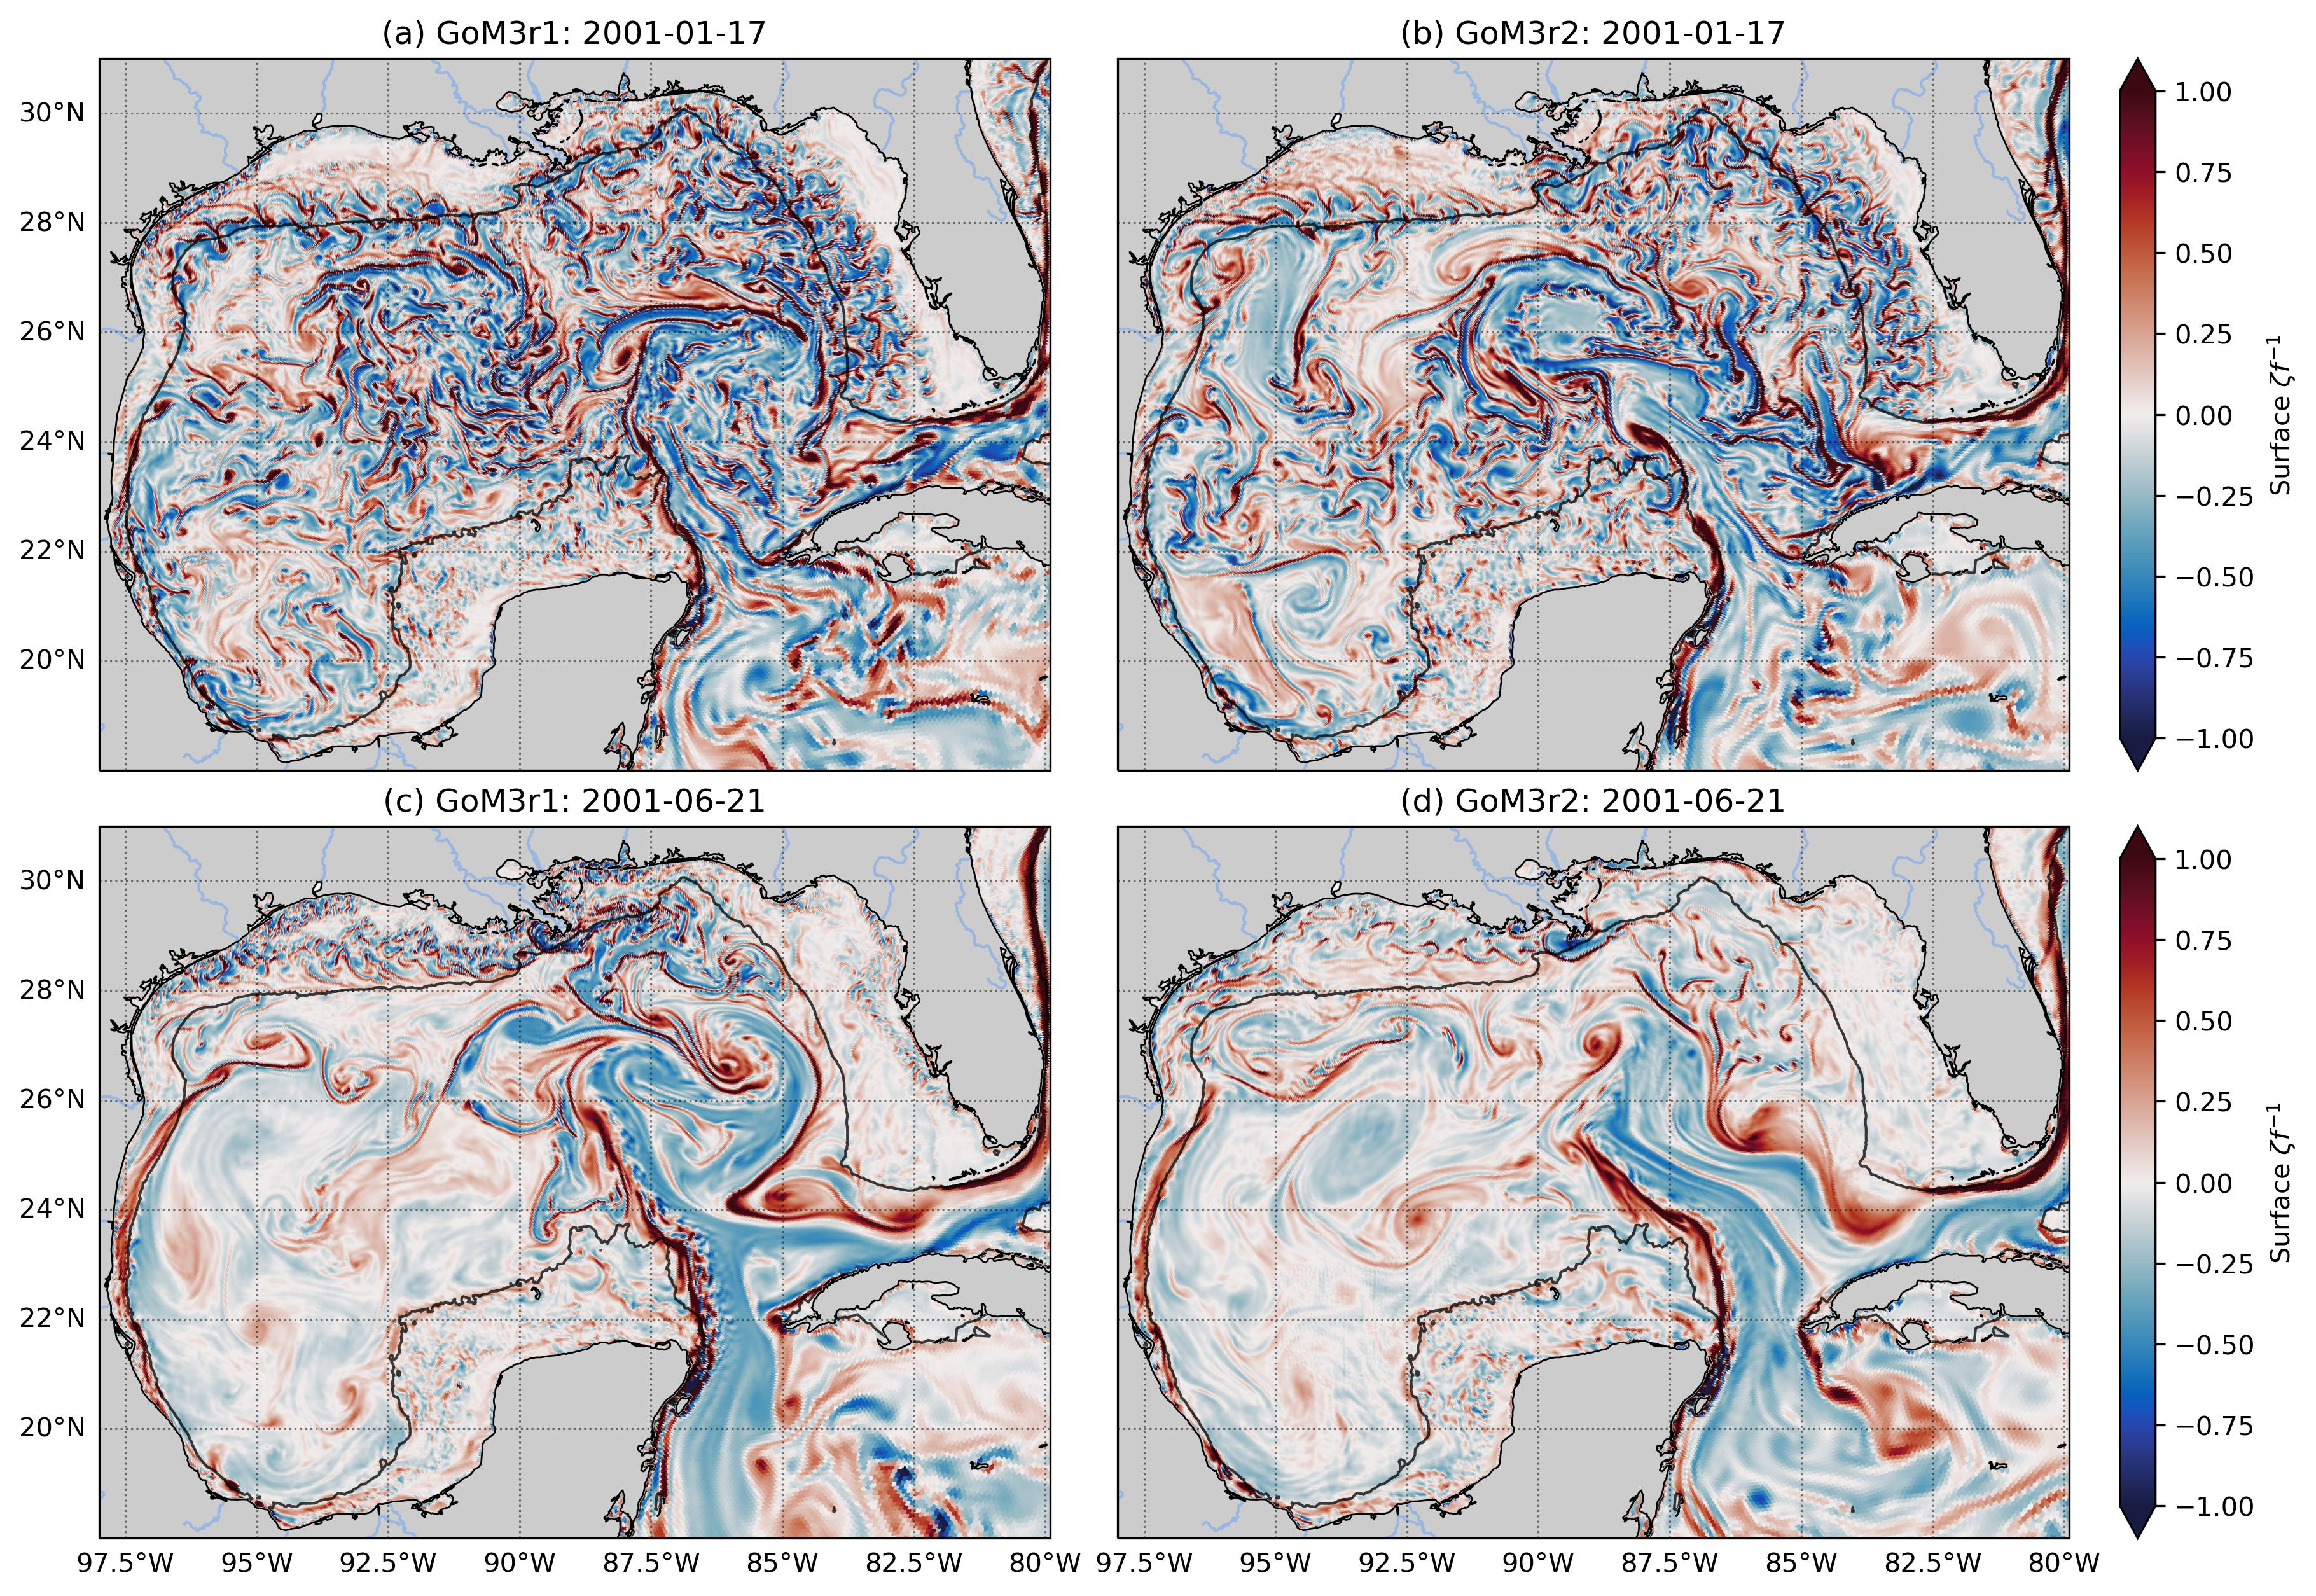
\includegraphics[width=\textwidth]{figures/scgsr/GoM3_rvort_comp2.jpg}}
    \caption{Snapshots of GoM3r1 (a) and GoM3r2 (b) surface $\zeta f^{-1}$ on Jan. 17, 2001. (c-d) same as (a-b), but on Jun. 26, 2001. The 100 m isobath is overlaid in black to show the shelf boundary.}
    \label{fig:gom3_rvort_planview}
\end{figure}

We examine the statistical representation of submesoscales in the GoM3 simulations using probability density functions (PDFs) of surface $\zeta f^{-1}$ for the entire GoM and TXLA shelf (Fig. \ref{fig:pdfs_gom}). The TXLA shelf is subsetted to the location of the child grid shown in \cite{Schlichting23} because frontal eddies are commonly found in this region. The prevalence of submesoscales are often indicated by elongated positive tails (cyclonic vorticity) in the PDF and a peak negatively offset from zero (anticyclonic vorticity) \citep{McWilliams_2016, Shcherbina_2013, taylor2023submesoscale}. Based on previous TXLA model results \citep{Schlichting23}, we anticipate a peak offset that is more pronounced over the shelf because the anticyclonic cores of frontal eddies saturate the shelf. 

\begin{figure}[t]
\centerline{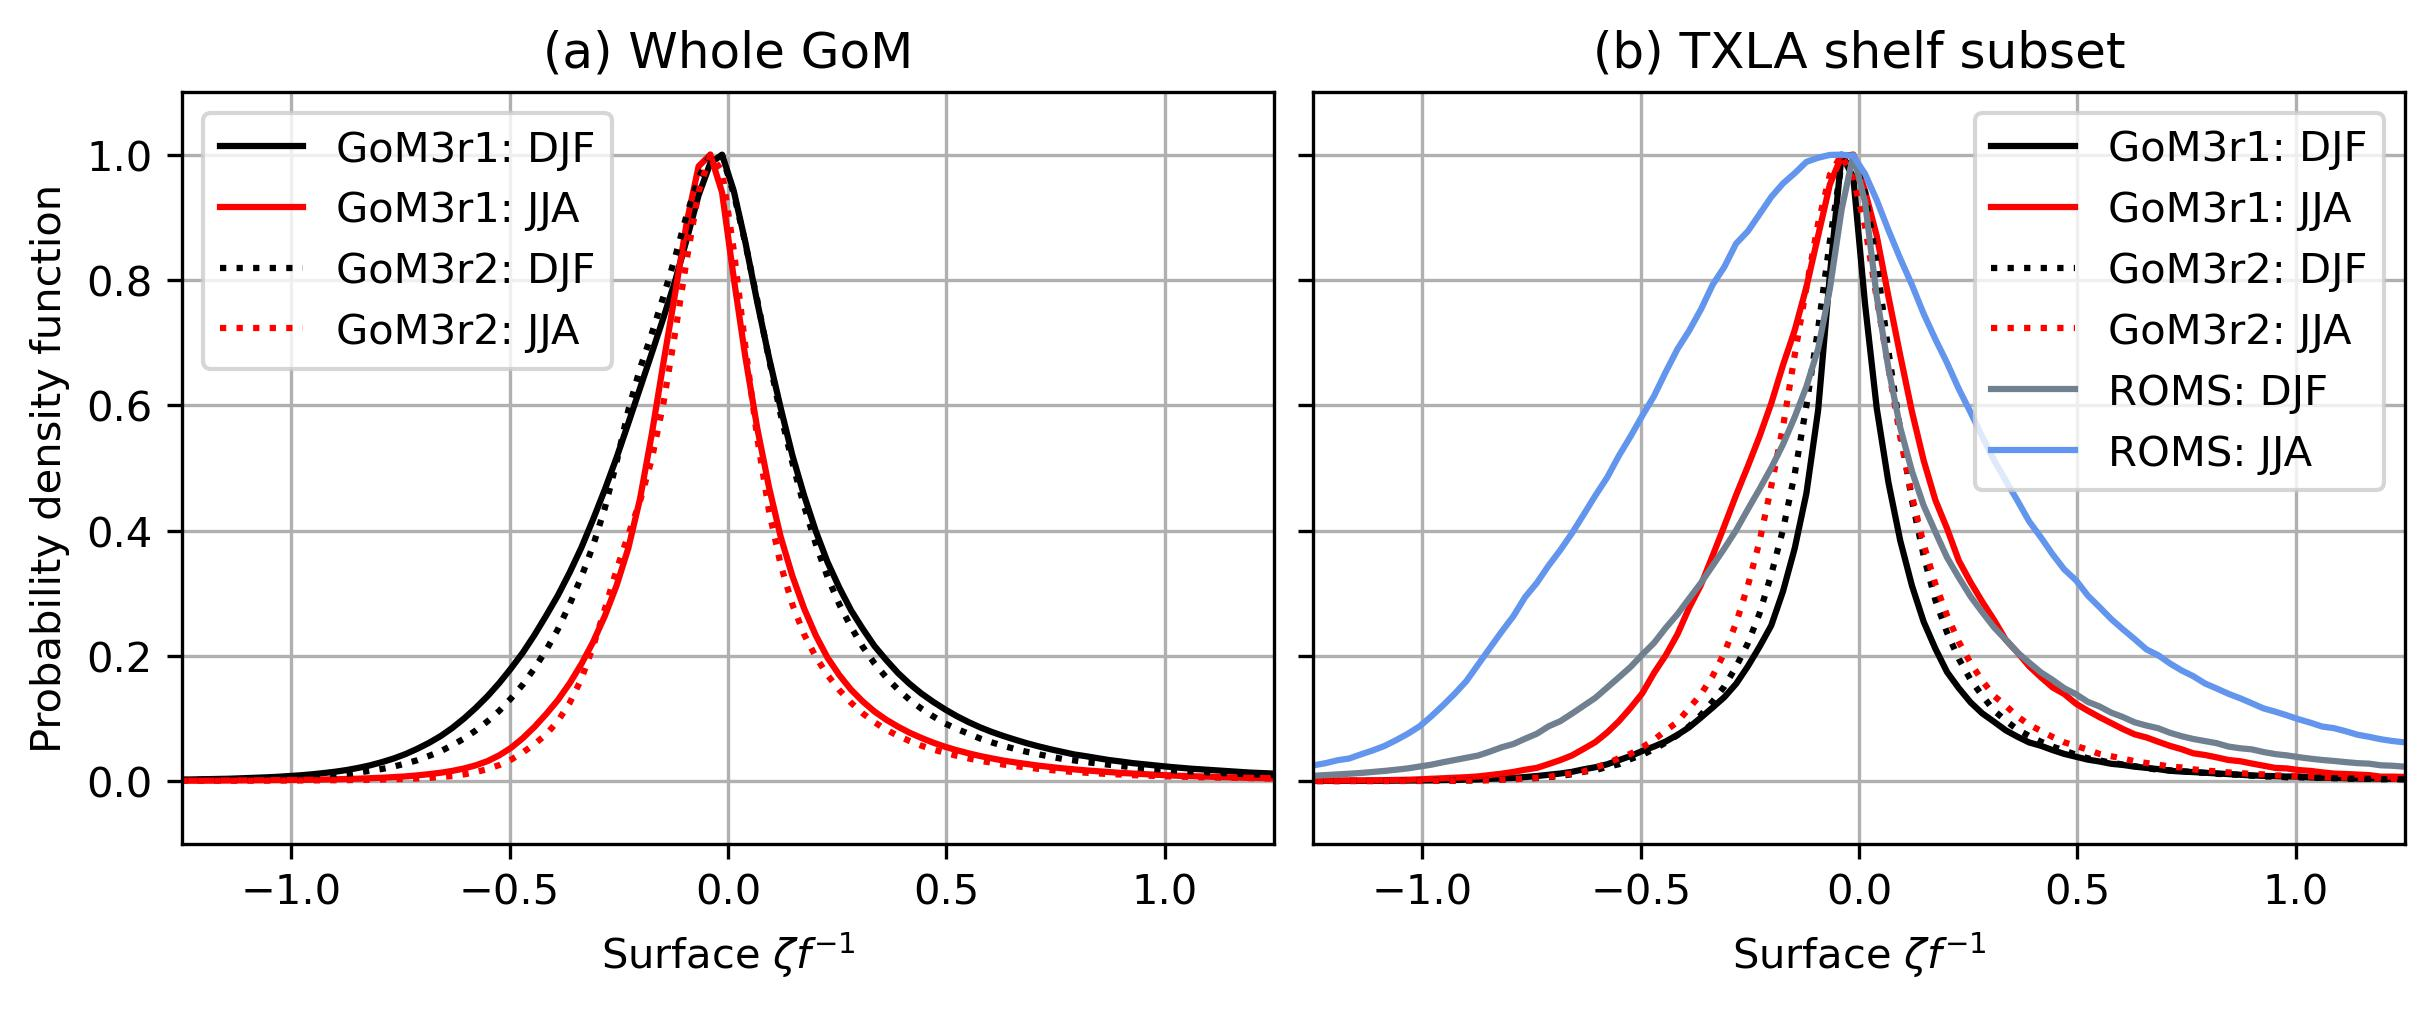
\includegraphics[width=\textwidth]{figures/scgsr/mpaso_roms_vortpdf.jpg}}
    \caption{Winter and summer probability density functions of surface $\zeta f^{-1}$ for the entire GoM (a) and TXLA inner shelf (b). The TXLA ROMS model is included in (b) for comparison.}
    \label{fig:pdfs_gom}
\end{figure}

For the whole GoM (Fig. \ref{fig:pdfs_gom} a), the GoM3 simulations feature a peak slightly offset from zero and tails that are just starting to elongate. For GoM3r1 during winter, less than one in every thousand cells (i.e. $PDF<10^{-3}$) falls within $\zeta f^{-1} = [-1.65,2.0]$. There are instances of stronger vorticity in winter than summer, indicating submesoscales are more prevalant in winter, which is consistent with Fig. \ref{fig:gom3_rvort_planview}. PDFs of GoM3r1 and GoM3r2 are very similar, with slightly stronger values found in GoM3r1.

For the TXLA shelf, the TXLA model produces a positively skewed PDF in summer with a peak further offset from zero than any GoM3 simulation due to a rich baroclinic eddy field (not shown). In winter, fewer submesoscales are found, resulting in a more symmetric PDF. However, the TXLA model during winter features stronger vorticity than both GoM3 simulations. This is due to two reasons, the mean horizontal resolution of the TXLA model is about 1.5 km in the region where the PDFs are computed, and the GoM3 simulations never develop an eddy field. Another interesting result is that GoM3r1 features stronger vorticity over the shelf relative to GoM3r2 despite the very low vertical resolution. Thus, until we solve the stability issues, it is unclear to what extent MPAS-O can represent submesoscales over the TXLA shelf. 

\subsection{Structure of the M/A river plume}
Figs. \ref{fig:mpaso_sss}-\ref{fig:ROMS_sss} display seasonally averaged sea surface salinity (SSS) for winter and summer for the GoM simulations and TXLA model, respectively. Note that we consider the TXLA model to be the reference because the salinity field has been validated twice and the errors are unbiased \citep{Kobashi_2020, Zhang_2012_numerical}. The 33 psu isohaline is indicated by the black line, which marks the edge of the M/A River plume \citep{hetland2012integrated, thyng2018seasonal}. In addition, this comparison is intended for qualitative purposes only because the TXLA model is forced with ERA interim datasets, not JRA.

\begin{figure}
\centerline{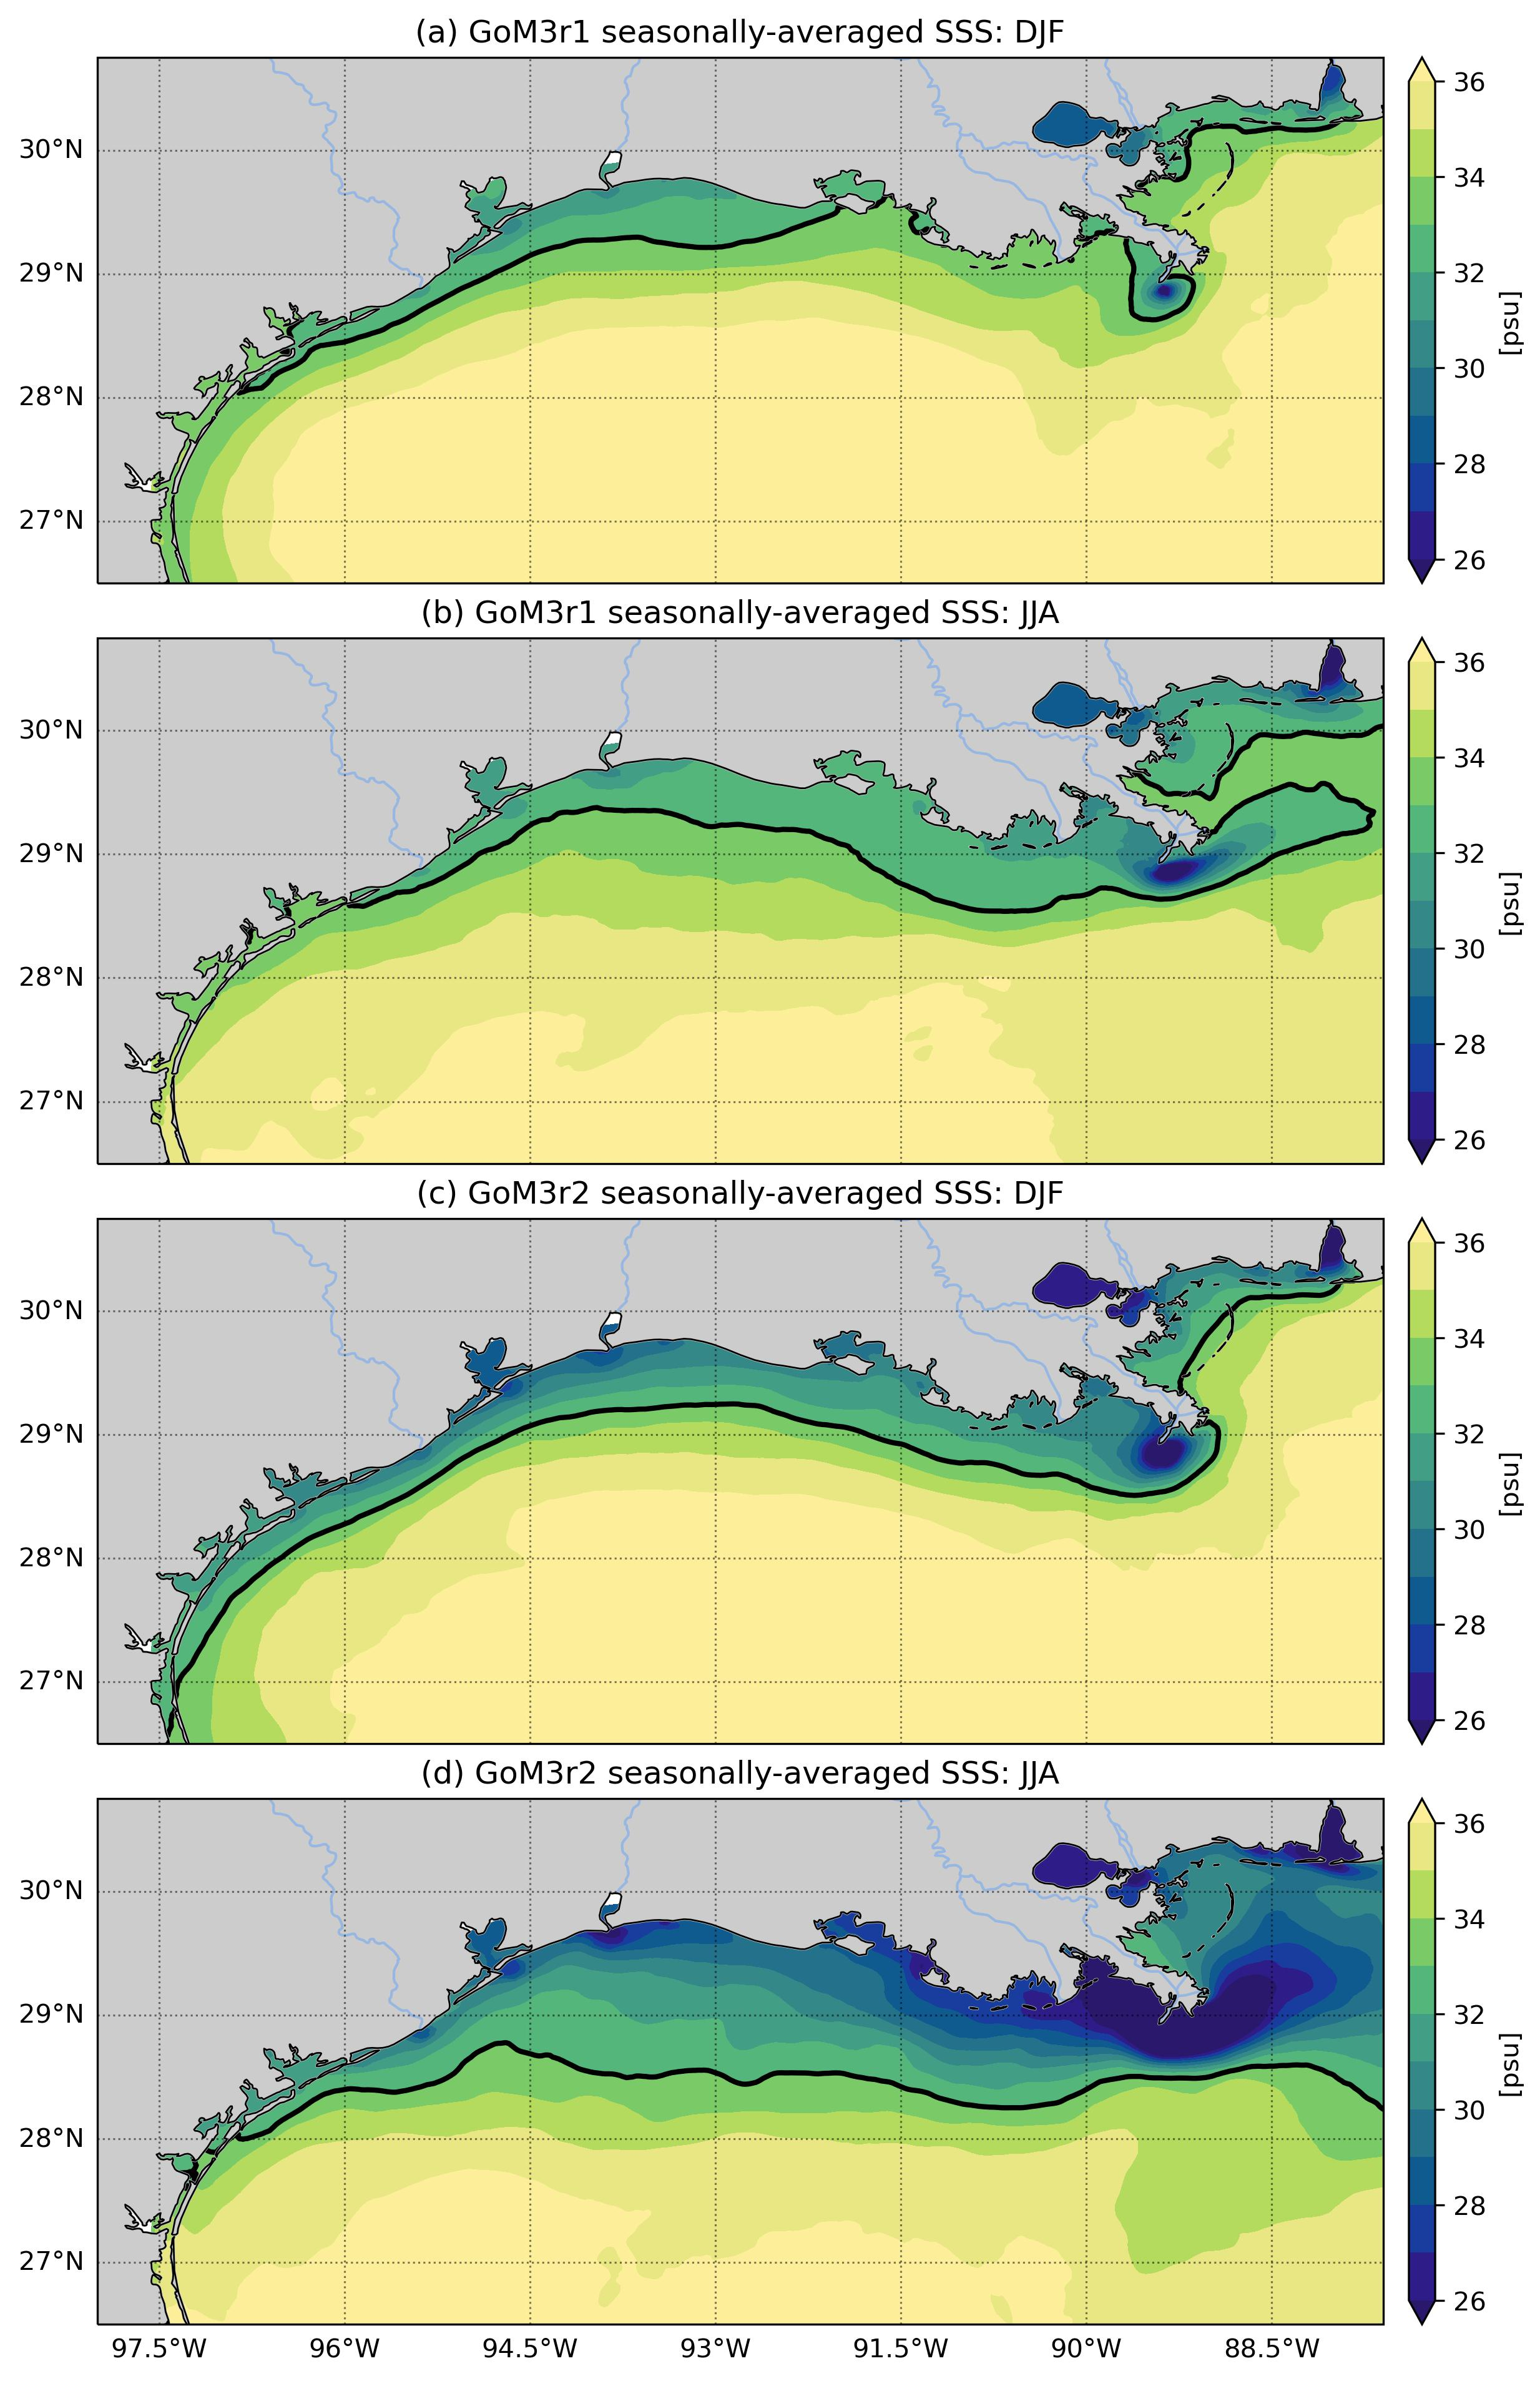
\includegraphics[width=0.82\textwidth]{figures/scgsr/mpaso_sss_mean.jpg}}
    \caption{Snapshots of the GoM3r1 seasonally averaged SSS for winter (a) and summer (b). (c-d) are the same as (a-b), but for GoM3r2. The black line marks the 33 psu isohaline.}
    \label{fig:mpaso_sss}
\end{figure}

\begin{figure}[t]
\centerline{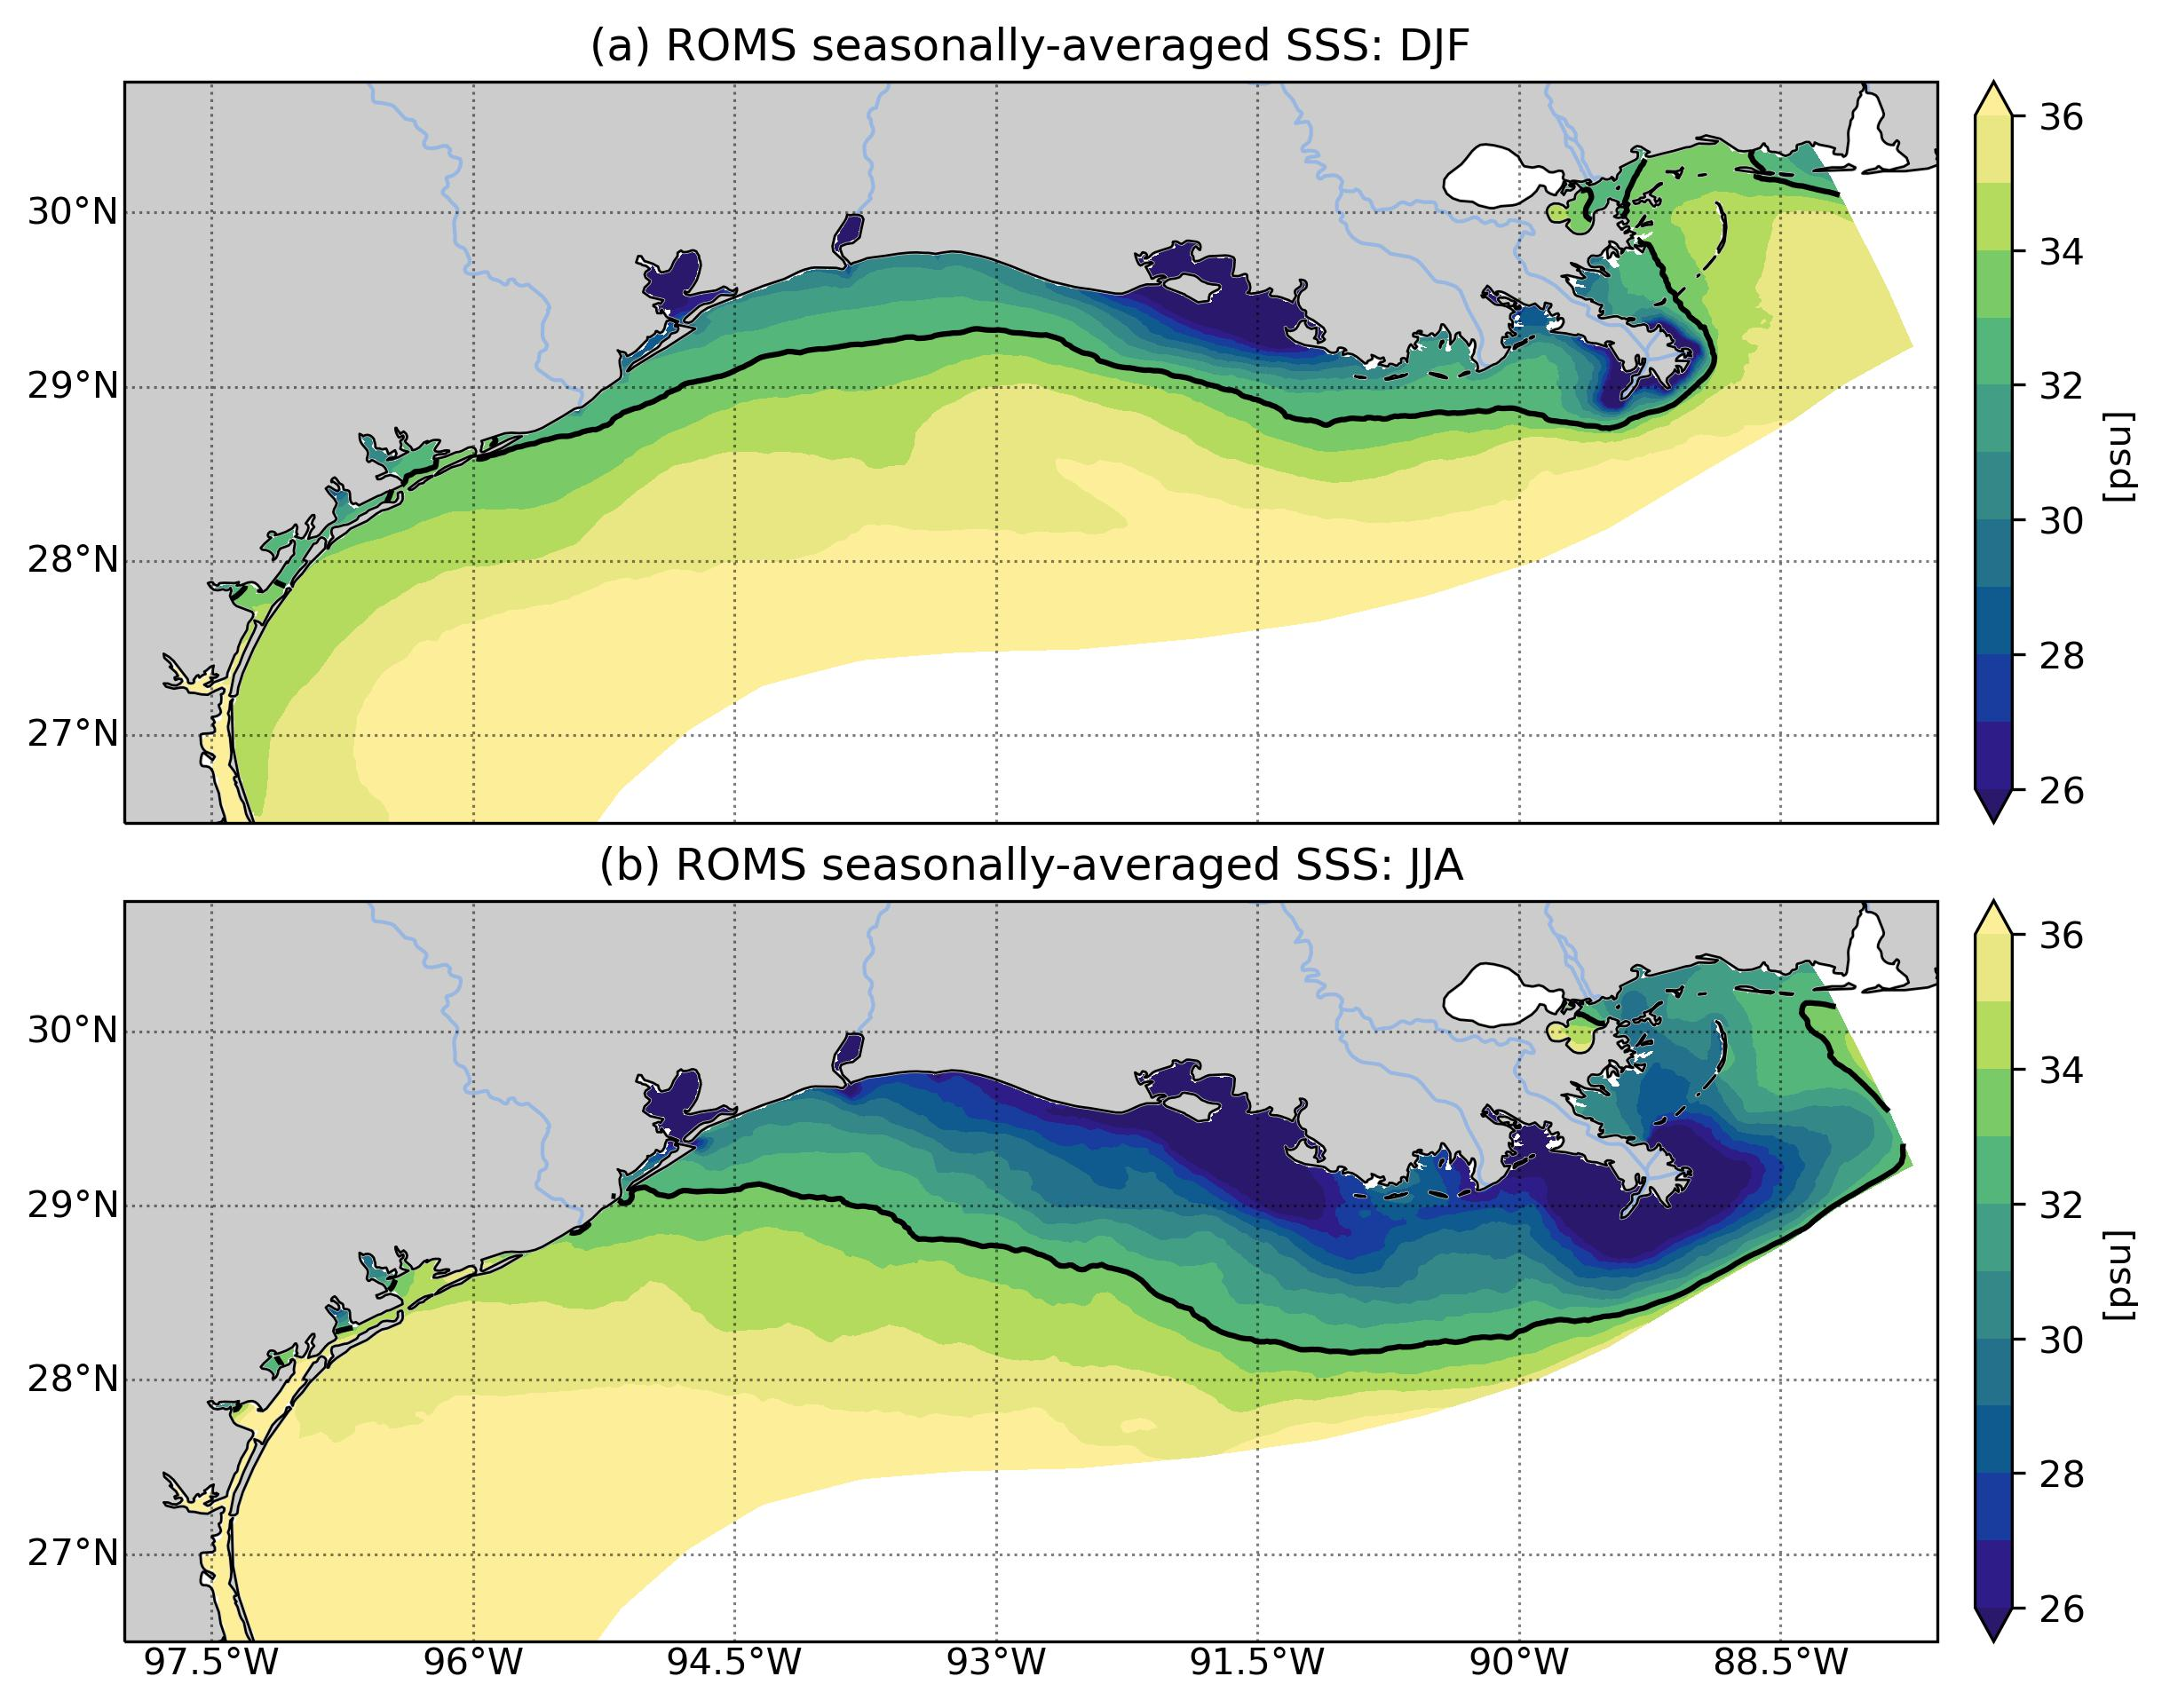
\includegraphics[width=0.82\textwidth]{figures/scgsr/txla_sss_mean.jpg}}
    \caption{Same as Fig. \ref{fig:ROMS_sss}, but for the TXLA model.}
    \label{fig:ROMS_sss}
\end{figure}

Despite the more "submesoscale" nature of GoM3r1's vorticity statistics, the river plume is poorly represented for both seasons and much of the shelf is too salty. This is an expected result given the low vertical resolution and the minimum water depth of 20 m. GoM3r2 produces a plume that is more qualitatively consistent with the TXLA model for both seasons and has a much more pronounced plume during summer relative to GoM3r1 despite not having an eddy field. However, we note that GoM3r2 is too salty in Atchafalaya Bay, along the other passes of Bird's foot, and near Port Arthur and Galveston Bay. In addition, GoM3r2 is too fresh over the western half of the TX shelf. 

We suspect the issues pertaining to Atchafalaya Bay and Bird's Foot are due to the lack of hydraulic control structure within JRA forcing and the river spreading still being too large, although this requires further investigation. That is, we suspect JRA forcing does account for United States Army Corps of Engineers modulation of Atchafalaya river fluxes. On the other hand, the TXLA model uses USGS streamflow data directly at the mouth of Atchafalaya Bay. Regarding the saltiness along the other passes of Bird's foot, this is because E3SM lacks a means to proportion the river fluxes through the other passes (as mentioned previously). Finally, we suspect the surplus of fresh water on the western TX shelf is because the river spreading is still too high, even with the newer spreading capabilities.

\section{Discussion and conclusions}
\subsection{Model strengths and limitations}
A current strength of the approach taken here is the GoM3 meshes have 345 thousand horizontal cells, which is low compared to other high resolution MPAS-O meshes \citep{caldwell2019doe, hoch2020mpas} and roughly three times as many horizontal cells as the TXLA model. This allows the quicker tuning of key subgrid scale parameterizations such as harmonic and biharmonic lateral mixing, GM, and Redi coefficients. However, this likely comes at the cost of being able to produce high-fidelity climate simulations. One solution is to regenerate the mesh and increase resolution outside the region of interest once the parameterizations have been tuned. Another strength is the representation of submesoscales within the broader GoM despite the coarse vertical resolution. The permission of seasonal variability is encouraging and we expect this to improve if higher horizontal resolution is used. 

The two biggest limitations preventing MPAS-O from being capable of producing high fidelity simulations of the TXLA shelf are vertical mesh stability issues and the river spreading. Notwithstanding stability issues, model fidelity is still constrained by river spreading. Although a river's spreading distance is set to be proportional to the inflowing flux, any spreading is physically unrealistic and will likely produce a fresh bias in most coastal regions. Even when individual river spreading is modified to be as small as stability constraints allow, it may be difficult or impossible to account for hydraulic control structures within the broader E3SM framework or when model forcing is run with reanalysis data. A potential option for future simulations is to incorporate rivers as point sources, as often done in many regional models. However, it is unclear if this could be done for stability reasons.

We note two experimental additions to the MPAS-O code that were not tested here but may be useful to future studies. One is the addition of a hybrid $\sigma-z$ vertical coordinate, which features a terrain following ($\sigma$) coordinate in the coastal ocean (the inner continental shelves/slopes) and transition to $z^*$ coordinates over the open open. The other addition is the inclusion of the Generic Length Scale (GLS) vertical mixing scheme configured as part of the General Ocean Turbulence Model \citep{burchard1999gotm, Warner_2005}, which has been shown to perform well in coastal models. 

In addition, we list several aspects of model configuration in approximate order of priority required to produce high fidelity simulations of coastal submesoscales that may be useful for future projects: 1) horizontal resolution, 2) vertical resolution, including an appropriate vertical coordinate for the region of interest, 3) realistic forcing, and 4) appropriately tuned subgrid-scale parameterizations. It should be noted that these components are inextricably linked and their order may differ depending on the project objectives. 

The horizontal resolution is the dominant factor affecting the resolved dynamics because it determines the Rossby number. High vertical resolution is necessary when the focus in on boundary- or mixed layer processes, and the vertical transport of material across- and within these layers. A heuristic argument can be made for the necessity of high quality forcing. The model will be as realistic as the forcing given to it. And finally, parameter tuning must be done on a per-mesh basis. Poorly tuned $\nabla_0^4$ can suppress submesoscales even if all other aspects of model configuration are optimized.

\subsection{Regional refinement compared to model nesting}
An alternative to the approach taken here is to one-way nest a regional model like ROMS into MPAS-O, which is currently being undertaken by the SEAHOR\c{C}E project (\url{https://github.com/seahorce-scidac}). An advantage of this approach is that ROMS is a mature regional ocean model specifically designed for simulations of estuarine and coastal flows with well understood strengths and limitations. Additionally, decades of work have gone into tuning and calibrating ROMS for the GoM region, while E3SM has historically had a more global focus to date. ROMS also features several options for tracer advection and vertical turbulence closure schemes in addition to KPP that can be experimented with to improve model performance. Particularly relevant for this work is that tracers can be treated as point sources such that anthropogenic hydraulic controls at discharge points can be easily accounted for. ROMS is also not prone to stability issues when run at high vertical resolution.

Besides creating robust code infrastructure to do the nesting, a major expected limitation of this approach is the computational cost. Model nesting has a additional computational overhead because information must be calculated at the lateral boundaries of each timestep and the inter-grid communication performance is dependent on a machine's hardware. The child grid will also require a finer timestep, which will slow computational speed. There is a similar issue in regionally refined MPAS-O meshes because the same timestep is applied to all cells. A possible remedy is to expand the local time stepping scheme \citep{lilly2023storm} to baroclinic applications. For the current MPAS-O code base, regional refinement appears to be a more practical option for open ocean regions (e.g. the Gulf stream) that are not signficantly influenced by river forcing and do not require $\mathcal{O}$(0.1 m) vertical resolution. These two approaches can be better compared when performance tests for nesting ROMS into MPAS-O are available. 

\section{Conclusions and future work}
We presented the development of an unprecedented 2.8 km resolution regionally refined mesh in the Gulf of Mexico (GoM) using the Model for Prediction Across Scales-Ocean (MPAS-O). The mesh, named GoM3, is intended to assess the representation of coastal submesoscale processes over the Texas-Louisiana (TXLA) shelf and the broader GoM. Our case study approach is motivated by the pronounced submesoscale eddy field that develops over the Mississippi and Atchafalaya (M/A) River plume over the TXLA shelf during summer and the strong seasonal variability of submesoscales within the broader GoM. The lateral density gradients of both regions are strongly modulated by regional rivers and the larger-scale mesoscale circulation, so we think this represents a challenging test to study submesoscales with regionally refined meshes. Our benchmark for comparison is a validated implementation of the Regional Ocean Modeling System (ROMS), the TXLA model, which covers the TXLA shelf and outer continental slopes. 

The horizontal mesh is gradually relaxed to 60 km in the broader Atlantic and Southern Oceans and to 100 km in the Pacific and Indian Oceans. MPAS-O is coupled with MPAS-Sea Ice to produce a realistic Atlantic Meridional Overturning Circulation such that a realistic loop current is produced. The simulations are forced with Japanese 55 year reanalysis datasets (JRA). Preliminary results suggest this configuration is not suitable for long-term climate simulations due to the low resolution regions, but further testing is required. We described improvements made to how river forcing is applied in the model, including the spreading and inflowing temperatures. We also found the representation of submesoscales to be sensitive to the amount of prescribed biharmonic lateral mixing. 

We ran two coupled numerical simulations using a low (GoM3r1) and medium (GoM3r2) vertical resolution mesh from 2000-2001 following a two year spinup. We were unable to produce a vertical mesh with comparable resolution and minimum bathymetry to the TXLA model due to stability issues. Both simulations do not produce a submesoscale eddy field over the TXLA shelf. However, they both permit submesoscales in the broader GoM and begin to produce seasonal variability found in previous studies \citep{Barkan_2017, liu2021submesoscale}. GoM3r1 produces a low quality representation of the M/A river plume due to the coarse vertical resolution, but has slightly more submesoscale features in the broader GoM than GoM3r2. This is because GoM3r2 required twice the biharmonic mixing as GoM3r1 to maintain stability. Despite the lack of submesoscale eddies, seasonal averages of sea surface salinity showed GoM3r2 produced a higher quality M/A river plume structure that starts to resemble the TXLA model. Major issues are over a salty bias near Atchafalaya Bay and a fresh bias off the southern TX coast, which we suspect is related to issues with river spreading and a lack of hydraulic control structure within JRA forcing. We plan to take several actions in future work described below to improve MPAS-O's representation of submesoscales over the TXLA shelf.

Assuming the vertical stability issues can be fixed, our next GoM3 simulation will target a 0.5 m minimum layer thickness and five m minimum water depth so it is comparable with the TXLA model. We will reduce the Atchafalaya River spreading to be similar to the Mississippi and examine where JRA forcing accounts for the hydraulic control structure over the M/A rivers. We also plan to generate a new horizontal mesh with 1.5 km resolution so it is comparable with the TXLA model in the region of interest. This will also allow us to compare model results in the broader GoM directly with previous studies that have already produced simulations at this resolution \citep{Barkan_2017, bracco2019mesoscale, liu2021submesoscale}. Ideally, we will run the TXLA model with JRA forcing so it can be compared directly with MPAS-O, which is especially important if JRA forcing lacks the hydraulic control between the M/A rivers. 

Regarding analysis, we will implement an idealized passive tracer that is intended to serve as a proxy for freshwater content over the shelf. We will compare monthly-averaged seasonal sections of the active and passive tracers between models, which can allow us to infer information abut the performance of KPP in coastal settings. We plan to add the approach by \cite{Klingbeil_2014} to quantify numerical mixing, the spurious mixing generated by the discretization of advection, to the MPAS-O code. Little work has been done in quantifying numerical mixing in MPAS-O simulations besides the approach by \cite{winters1995available}, which is restricted to reference potential energy integrated over entire control volumes.

		% Include the Section4.tex file --- Chapter 3
% !TEX root = ../TAMU_Thesis_Main.tex

%%%%%%%%%%%%%%%%%%%%%%%%%%%%%%%%%%%%%%%%%%%%%%%%%%%%%%%%%%%%%%%%%%%%%%
%%                           SECTION V
%%%%%%%%%%%%%%%%%%%%%%%%%%%%%%%%%%%%%%%%%%%%%%%%%%%%%%%%%%%%%%%%%%%%%

\chapter{SUMMARY AND CONCLUSIONS \label{cha:Summary}}
This dissertation used a case study approach to explore numerical and physical salinity mixing in realistic and idealized simulations of submesoscale baroclinic instabilities with the Regional Ocean Modeling System (ROMS). The study site was the Mississippi and Atchafalaya (M/A) River plume over the Texas Louisiana (TXLA) shelf in the northern Gulf of Mexico (nGoM). The region is a known hotspot for submesoscales during summer as frontal eddies are squeezed and stretched by lateral buoyancy forcing from regional rivers and the passage of occasional storms. Many of the research questions outlined in Section \ref{sec:diss_obj} are novel because numerical mixing has not been characterized in submesoscale eddy-resolving simulations. Our findings from two studies are summarized below, with two major conclusions drawn per study. 

First, we used a non-nested version of the realistic TXLA model to characterize whether numerical mixing can be quantified offline with the residuals of the volume-mean salinity variance ($s^{\prime^2}$) and salinity squared ($s^2$) budgets. The accuracy of offline methods were evaluated with an analogous online method. We found the accuracy of the offline methods to be strongly dependent on the model output frequency. At an output frequency of one hour, numerical mixing estimated from the $s^2$ budget is noisy and can disagree with the online method by over an order of magnitude. For the same output frequency, numerical mixing estimated from the $s^{\prime^2}$ budget overestimated the online method by 60\%. Increasing the output frequency to ten minutes did not substantially change the accuracy of numerical mixing estimated from the $s^{\prime^2}$ budget. Thus, we found that offline methods should not be used to quantify numerical mixing because they did not converge to the online method even as the output frequency is increased to ten minutes, which is impractical for long term coastal simulations. 

Second, we used a two-way nested version of the TXLA model to quantify the sensitivity of numerical and physical mixing to horizontal resolution. We found that volume-integrated numerical mixing comprised 57\% of the physical mixing in the non-nested model. Volume-integrated numerical mixing generally decreased and physical mixing increased as grid resolution increased. We increased grid resolution by a factor of five, which caused numerical mixing to decrease by 35\% and physical mixing to increase by 42\%. Numerical mixing was roughly proportional to the magnitude of horizontal salinity gradients, which were strongest at ocean fronts. The across-frontal length scales generally decreased as model resolution increases, so the integrated amount of numerical mixing decreased. However, increased resolution can resolve new processes that create new horizontal gradients, or further sharpen existing gradients via frontogenesis. Thus, increasing resolution may have diminishing returns for reducing numerical mixing once a model permits submesoscales. Increased resolution caused physical mixing to increase because newly resolved processes created new sources of salinity variance that can be mixed. New processes also increased the vertical velocity variance of the flow, which caused the salinity diffusivity calculated from the turbulence closure scheme to increase. 

Third, we used an idealized submesoscale eddy-resolving model of the TXLA shelf to show that numerical mixing can dominate physical mixing in frontal zones. We showed this by comparing volume-integrated numerical and physical mixing for several depth ranges. When integrating over the top one meter of the water column, which is where fronts are most prevalent, bulk estimates of numerical mixing were over twice as large as physical mixing. In addition, joint probability density functions of the surface normalized frontogenesis function and numerical mixing showed that numerical mixing is elevated throughout a front's life cycle. That is, numerical mixing is stronger when fronts are being sharpened by frontogenesis or destroyed by frontolysis compared to fronts that undergo neither process. 

Fourth, we varied the tracer advection scheme in an ensemble with the idealized model to investigate the impacts of numerical mixing on the larger scale ocean circulation and tracer state. A key result was that the scheme (HSIMT) with the most numerical mixing damped the release of available potential energy by partially suppressing baroclinic instabilities. The strongest evidence for this is the ensemble-averaged eddy kinetic energy in the HSIMT runs was 25\% lower than runs in the scheme (MPDATA) with less than half the numerical mixing. The suppression of instabilities caused biases in alongshore-averaged salinity sections exceeding 0.75 g kg$^{-1}$ in just 30 days. We expect tracer field biases caused by numerical mixing to be much larger in realistic simulations that run simulations for much longer. These results suggested that numerical mixing continues to affect model fidelity even at submesoscale-resolving resolution. 

After answering the research questions pertaining to numerical mixing, we used the knowledge gained from the TXLA model simulations to present preliminary developments of a submesoscale eddy-permitting regionally refined mesh in the GoM using the Model for Prediction Across Scales Ocean (MPAS-O). MPAS-O is the global ocean component of the Department of Energy's Energy Exascale Earth System Model. This study was the first to assess MPAS-O's representation of submesoscale processes. Our assessment focused on the seasonal variability  of surface submesoscales in GoM and the structure of M/A river plume. We presented simulations with low and medium vertical resolutions that were run for two years (2000-2001) and compared with the non-nested TXLA model. We were unable to produce a high vertical resolution case because the model experiences stability issues near the M/A discharge points. We plan to fix these stability issues moving forward. 

While both simulations permitted submesoscale seasonal variability in the broader GoM, they poorly represented submesoscales over the TXLA shelf and did not produce an eddy field during summer. In addition, both simulations demonstrated major differences in seasonally averaged sea surface salinity relative to the TXLA model. We anticipate improved performance with MPAS-O once the stability issues are fixed and the river forcing is further adjusted. 

The unifying theme of this dissertation is that we studied several factors that affect numerical model fidelity. As George Veronis showed back in the 1970's, just one poorly implemented or untuned subgrid-scale parameterization can cause numerical models to drift away from reality. We primarily focused on numerical mixing with the TXLA model, but also show this with several aspects of model setup and configuration during the MPAS-O study. While numerical mixing is not a parameterization, it can be argued that partially represent unresolved processes because it is controlled by truncation error. We hope that future studies may use the knowledge gained from this work to develop methods that minimize numerical mixing in primitive equation ocean models. 


       % Include the Section5.tex

%%%%%%%%%%%%%%%%%%%%%%%%%%%%%%%%%%%%%%%%%%%%%%%%%%%%
% Generate the Bibliography DO NOT TOUCH THIS!!!
\makebibliography

%%%%%%%%%%%%%%%%%%%%%%%%%%%%%%%%%%%%%%%%%%%%%%%%%%%%
% Include appendices. 
% MUST BE IN APPENDICES ENVIRONMENT!!!
\begin{appendices}
    % % !TEX root = ../TAMU_Thesis_Main.tex

% %%%%%%%%%%%%%%%%%%%%%%%%%%%%%%%%%%%%%%%%%%%%%%%%%%%%%%%%%%%%%%%%%%%%%%
% %%                           APPENDIX A 
% %%%%%%%%%%%%%%%%%%%%%%%%%%%%%%%%%%%%%%%%%%%%%%%%%%%%%%%%%%%%%%%%%%%%%

% \phantomsection
\chapter{Appendix for Quantification of physical and numerical mixing in a coastal ocean model using salinity variance budgets}%\label{appendix:01}

\section{Numerical implementation of the offline method} %\label{Appendix:offline_method}

Here, we provide details of the numerical implementation of Eq. \ref{eq:salt2_mnum} and Eq. \ref{eq:sprime2_mnum} for the case of hourly model output. We used average files to construct the volume-integrated $s^2$ and $s^{\prime^2}$ budgets, which output averages of all variables between each hour. The implementation is shown for a 3D control volume $V$ larger than one discrete water column. Spatial indices are denoted with subscripts $i,j,k$ corresponding to the $x,y,z$ directions with temporal index $n$. Calculations at the cell centers are denoted with whole indices. Calculations on the center of cell edges are denoted with half indices. 

Starting with the volume-integrated $s^2$ budget, the tendency term $\mathrm{Tend}^n$ was calculated as
\begin{equation} \label{eq:append_tend}
        \mathrm{Tend}^n = \sum_{i=1}^{I}\sum_{j=1}^{J}\sum_{k=1}^{K} \frac{\partial_t \left(\delta_{i,j,k}^n \left(s_{i,j,k}^{n} \right)^2 \right)}{\delta_{i,j,k}^n} \, dV \quad ,
\end{equation}
where $\partial_t$ denotes a centered finite difference, i.e., 
\begin{equation} \label{eq:append_finitediff}
        \partial_t \left(\delta_{i,j,k}^n \left(s_{i,j,k}^{n} \right)^2 \right) = \frac{\delta_{i,j,k}^{n+1} \left(s_{i,j,k}^{n+1} \right)^2-\delta_{i,j,k}^{n-1} \left(s_{i,j,k}^{n-1} \right)^2}{2 \Delta T} \quad ,
\end{equation}
where $\delta_{i,j,k}^n$ is the vertical layer thickness, $(s_{i,j,k}^{n})^2$ is the salt squared and $\Delta T$ is the model output frequency, not to be confused with the model timestep (e.g, Eq. \ref{Eq:mnum_online}). $\mathrm{Tend^n}$ is discretized as the volume integral of the time rate of change of the total $s^2$ content in a cell divided by the cell thickness. We computed the tendency terms in this form because the offline method consistently yielded better agreement between $\mathcal{M}_{num,s^2}$, $\mathcal{M}_{num,s^{\prime^2}}$, and $\mathcal{M}_{num,on}$. 

There are several methods to compute the advection term $\mathrm{Adv^n}$. An advantage of using average files compared to model snapshots (history files) is that they include the volume-conserving fluxes Huon and Hvom, which are the volume fluxes through the $x$ and $y$ faces calculated online that are averaged over the specified output frequency. They are defined as
\begin{equation}
        \begin{split}
        \mathrm{Huon}_{i \pm 1/2,j,k}^n & = \left(DY_{i\pm 1/2,j} \right) \left(\delta_{i\pm 1/2,j,k}^n \right) \left(u_{i\pm 1/2,j,k}^n \right) \\
        \mathrm{Hvom}_{i,j \pm 1/2,k}^n & = \left(DX_{i,j\pm 1/2}\right)\left(\delta_{i,j\pm 1/2,k}^n\right)\left(v_{i,j\pm 1/2,k}^n\right) \quad ,
        \end{split}
\end{equation}
where $DY$ is the cell width in the $y$ direction and $DX$ is the cell boundary width in the $x$ direction. As \cite{MacCready_2016} note, using Huon and Hvom helps reduce errors when quantifying advection through the lateral boundaries. The boundary fluxes may also be computed offline without the volume-conserving fluxes, however there may be decrease in accuracy. \text{Adv}$^n$ is formulated such that fluxes out of the control volume are considered positive and was calculated as 
\begin{equation} \label{eq:append_adv}
        \begin{split}
        \mathrm{Adv}^n = \sum_{j=1}^{J}\sum_{k=1}^{K}\left(\text{Huon}_{i \pm 1/2, j,k}^n \right) \left(s_{i \pm 1/2,j,k}^{n} \right)^2 \bigg|_{W}^{E}+ \\ 
        \sum_{i=1}^{I}\sum_{k=1}^{K} \left(\text{Hvom}_{i,j \pm 1/2,k}^n \right) \left(s_{i,j \pm 1/2,k}^{n} \right)^2 \bigg|_{S}^{N}
        \end{split}    
\end{equation}

where $E,W,N,S$ denote the east, west, north, and south boundaries of the control volume, respectively. The half indices in this case correspond to the centers of cell edges at the lateral boundaries. To expand the $\pm$ notation, $(s_{i-1/2,j,k}^{n})^2$ corresponds to $s^2$ at the western boundary of the control volume, $(s_{i+1/2,j,k}^{n})^2$ corresponds to the eastern boundary, $(s_{i,j-1/2,k}^{n})^2$ corresponds to southern boundary, and $(s_{i,j+1/2,k}^{n})^2$ corresponds to the northern boundary. 

The surface $s^2$ flux $\mathrm{surf}^n$ was calculated as
\begin{equation} \label{eq:append_surf}
        \mathrm{surf}^n = \sum_{i=1}^{I}\sum_{j=1}^{J}(2s_{i,j}^n)(s_{i,j}^n) \left(\frac{E_{i,j}^n-P_{i,j}^n}{\rho_w} \right) \, dA
\end{equation}

where $E_{i,j}^n$ and $P_{i,j}^n$ are the evaporation and precipitation per unit area (``Evaporation" and ``Rain" in ROMS output) computed online as part of the model forcing, and $\rho_w$ is the density of freshwater set to a constant value of 1000 kg m$^{-3}$. 

The volume-integrated horizontal diffusion $\mathrm{Hdiff}^n$ was calculated as
\begin{equation}
    \begin{split} \label{eq:append_hdiff}
            \mathrm{Hdiff}^n = \sum_{i=1}^{I}\sum_{j=1}^{J}\sum_{k=1}^{K} \partial_x \left[ \left(\kappa_{H,i \pm 1/2,j} \right) \left(\partial_x \left(s_{i,j,k}^{n} \right)^2 \right) \right] + \\ \partial_y \left[\left(\kappa_{H,i,j \pm 1/2} \right) \left(\partial_y \left(s_{i,j,k}^{n} \right)^2 \right) \right] \, dV \quad ,
    \end{split}
\end{equation}

where $\kappa_{H,i,j}$ is the horizontal turbulent diffusivity computed offline defined in Eq. \ref{eq:kappa_H}. $\kappa_{H,i,j}$ was first linearly interpolated to the centers of cell edges to align the model grid after computing horizontal derivatives $\partial_x$ and $\partial_y$ of $s^2$, which are calculated using a Jacobian to account for the change of the sea surface height with respect to time \citep{shchepetkin2005regional}. Further details of the Jacobian calculation may be found in \citet{xroms}. 

The resolved vertical mixing $(\chi_v^s)^n$ was calculated online so discretization errors do not bias comparisons with $\mathcal{M}_{num, on}$. $(\chi_v^s)^n$ was calculated as 
\begin{equation} \label{eq:append_vmix}
        (\chi_v^s)^n = \sum_{i=1}^{I}\sum_{j=1}^{J}\sum_{k=1}^{K} \mathrm{Vert. \, Mix}_{i,j,k}^n \, dV,
\end{equation}
where $\mathrm{Vert. \, Mix}_{i,j,k}^n$ is the resolved vertical mixing, denoted by ``$\mathrm{AKr}$" in ROMS syntax (not to be confused with $\mathrm{AKs}$, the resolved vertical salinity diffusion coefficient). $\mathrm{AKr}$ was linearly interpolated to the cell centers of the vertical grid prior to integration. We note that offline calculations of $(\chi_v^s)^n$, although not used in this study, tended to overestimate the online calculations.

The resolved horizontal mixing $(\chi_H^s)^n$ was computed offline because it is not currently programmed into the ROMS source code. It is also much smaller than other terms for our model, so offline discretization errors do not significantly impact $\mathcal{M}_{num, s^2}$.  $(\chi_H^s)^n$ was calculated as
\begin{equation} \label{eq:append_hmix}
        (\chi_H^s)^n = \sum_{i=1}^{I}\sum_{j=1}^{J}\sum_{k=1}^{K} 2\kappa_{H,i,j} \left[ \left(\partial_x s_{i,j,k}^n \right)^2+\left(\partial_y s_{i,j,k}^n \right)^2 \right]  \, dV.
\end{equation}

Horizontal gradients were calculated using a Jacobian but then interpolated to cell centers for both horizontal and vertical grids. Once calculated, the above terms may be substituted into Eq. \ref{eq:salt2_mnum} to obtain $\mathcal{M}_{num, s^2}$.

The process for discretizing the volume-mean salinity variance budget is similar, but requires calculation of the volume-averaged salinity $\overline{s}^n$. $\overline{s}^n$ was calculated as
\begin{equation}
        \overline{s}^n = \frac{1}{V^n} \sum_{i=1}^{I}\sum_{j=1}^{J}\sum_{k=1}^{K} s_{i,j,k}^n \, dV \quad .
\end{equation}

The volume-mean salinity variance $(s_{i,j,k}^{{\prime^2}})^n$ may be calculated as
\begin{equation}
        \left(s_{i,j,k}^{{\prime^2}} \right)^n = \left(s_{i,j,k}^n-\overline{s}^n \right)^2.
\end{equation}

The terms in Eq. \ref{eq:sprime2_mnum} may be calculated by substituting $(s_{i,j,k}^{\prime})^n$ and $(s_{i,j,k}^{\prime^2})^n$ where applicable into Eqs. \ref{eq:append_tend}-\ref{eq:append_finitediff} and Eqs. \ref{eq:append_adv}-\ref{eq:append_hdiff}. Recalculation of the physical mixing terms is not required because $\overline{s}^n$ has no spatial gradients.

\newpage
% % % \KOMAoptions{paper=portrait,pagesize}
% % % \recalctypearea
% \section{References for Appendix}
% % %%% Manually add references after each section
% \bibliographystyle{apalike}
% \begingroup
% % \renewcommand{\section}[2]{}%
% \bibliography{references}
% \endgroup

			% Include the appendix1.tex file
    % % !TEX root = ../TAMU_Thesis_Main.tex

% %%%%%%%%%%%%%%%%%%%%%%%%%%%%%%%%%%%%%%%%%%%%%%%%%%%%%%%%%%%%%%%%%%%%%%
% %%                           APPENDIX B
% %%%%%%%%%%%%%%%%%%%%%%%%%%%%%%%%%%%%%%%%%%%%%%%%%%%%%%%%%%%%%%%%%%%%%
\chapter{Appendix for Numerical mixing suppresses submesoscale baroclinic instabilities over sloping bathymetry}%\label{appendix:01}
\section{Ensemble of near-inertial wind amplitude} 

\begin{figure}[t]
    \begin{center}
    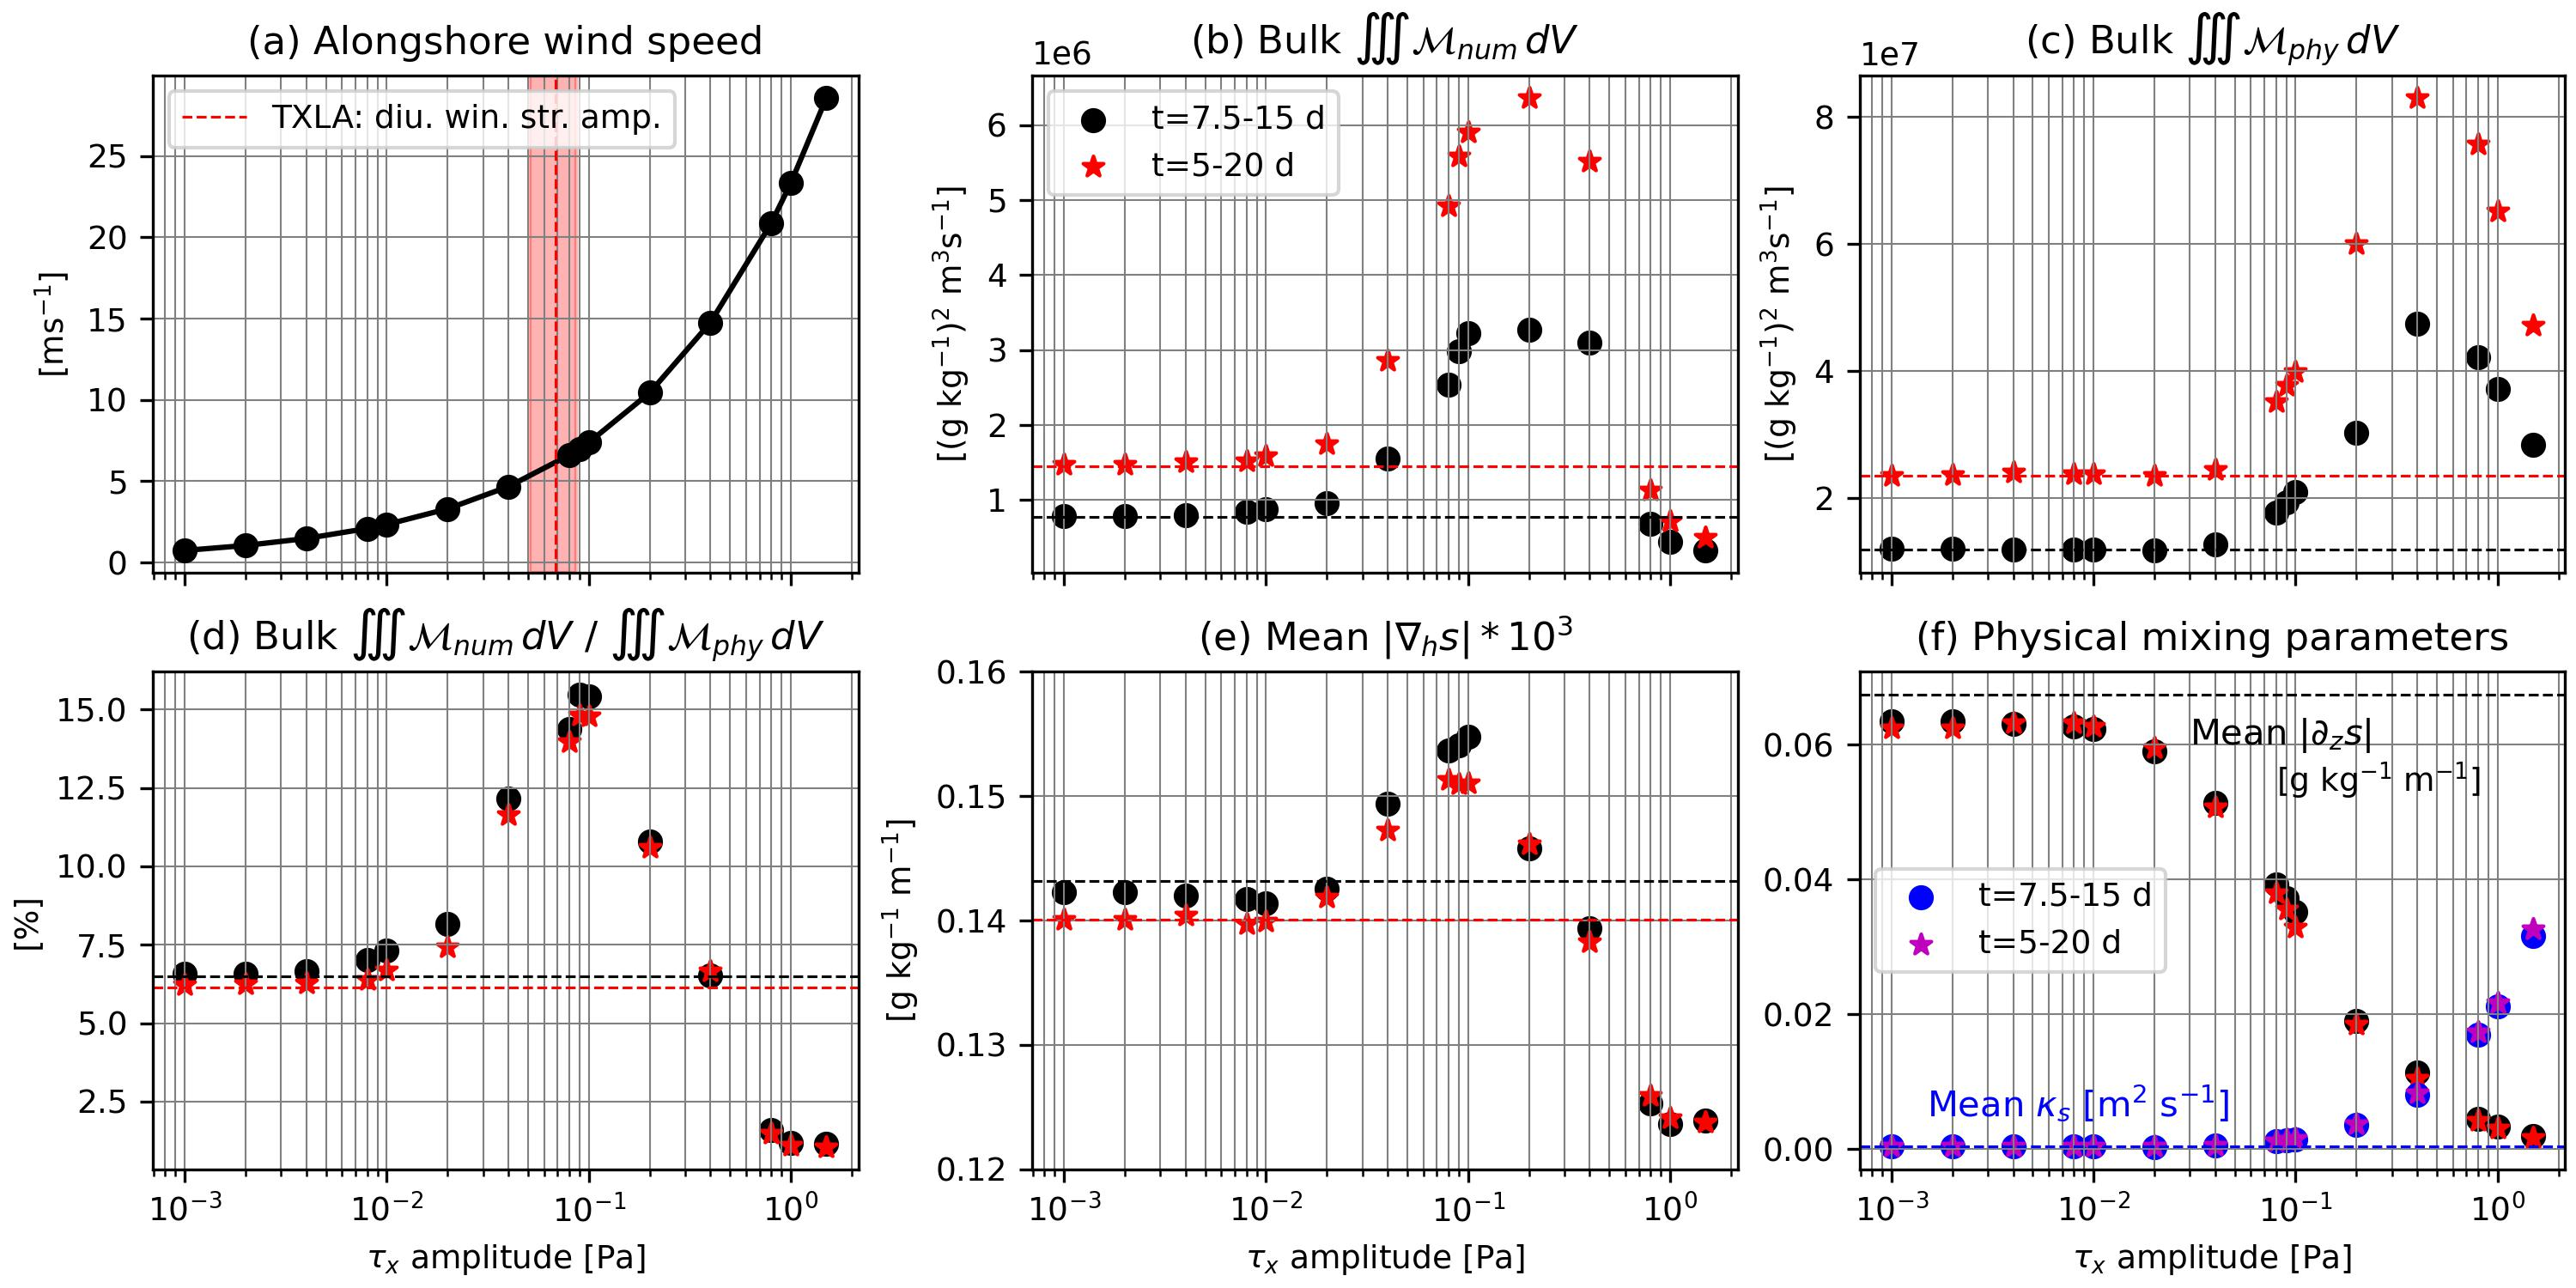
\includegraphics[width = \linewidth]{figures/shelfstrat_2024/mixing_function_taux.jpg}\\
    \caption{(a) Wind speed as a function of $\tau_0^x$ calculated using Eq. \ref{eqn:windspd}, with each dot representing a different numerical simulation. The amplitude of the diurnal wind stress magnitude spatially- and temporally averaged for the entire realistic simulation of the child domain \citep[see Fig. 7 a of] []{Schlichting23} with 95\% confidence intervals is shown with the red dashed line and shaded areas. Bulk $\mathcal{M}_{num}$ (b) and $\mathcal{M}_{phy}$ (c). (d) Ratio of bulk $\mathcal{M}_{num}$ to $\mathcal{M}_{phy}$ expressed expressed as a percent. Spatially- and temporally-averaged $|\nabla_h s|$ (e), $|\partial_z s|$ (f), and $\kappa_v$ (f). Quantities in (b)-(f) are calculated in the initially stratified region for two time periods and the horizontal dashed lines show unforced case values for their respective time periods coded by color.} \label{fig:wind_ensembles}
     \end{center}
\end{figure}

The impacts of varying the near-inertial alongshore wind stress amplitude $\tau_0^x$ on bulk mixing quantities associated with each ensemble member are shown in Fig. \ref{fig:wind_ensembles}. In addition, we show spatially- and temporally averaged parameters related to each mixing quantity to better understand how the bulk mixing quantities change in response to different $\tau_0^x$. To provide a sense of scale for $\tau_0^x$, we plot the amplitude of the wind speed $U_{wind}$ by solving the equation
\begin{equation} \label{eqn:windspd}
    \tau_0^x=\rho_a C_d U_{wind}^2 \, ,
\end{equation}
where $\rho_a$ is the density of air and $C_d$ is the drag coefficient set to a constant value of 0.0015. $U_{wind}$ of the ensemble runs span from $<1$ms$^{-1}$ to tropical storm force winds (29 ms$^{-1}$, until the model blew up). 

All bulk quantities are shown from days 5-20 and days 7.5-15 to indicate the trends are robust. The x-axes are on a log$_{10}$ scale. The time-averaged amplitude of the diurnal (inertial) wind stress magnitude from the realistic model \citep[Fig. 7 a of ][]{Schlichting23} is shown to contextualize the base case. The base case wind is slightly more energetic than the mean values observed during the realistic model simulation. The realistic surface forcing is highly variable, but spatially-averaged values rarely exceeded 10 ms$^{-1}$. 

$\tau_0^x$ values from $10^{-3}-10^{-2}$ Pa have little impact on volume-integrated $\mathcal{M}_{num}$ (Fig. \ref{fig:wind_ensembles} b) or $\mathcal{M}_{phy}$ (Fig. \ref{fig:wind_ensembles} c). As $\tau_0^x$ increases, $\mathcal{M}_{num}$ rapidly grows until plateauing from $\tau_0^x$=0.1-0.3 Pa, then rapidly decreases. In linear space, this qualitatively resembles a Chi-squared distribution with few degrees of freedom such that the peak is biased towards zero. The time- and spatially-averaged $|\nabla_h s|$ peaks at 0.1 Pa then begins to rapidly decrease (Fig. \ref{fig:wind_ensembles} e). As the wind stress amplitude approaches 1 Pa, winds suppress the instabilities, causing $\mathcal{M}_{num}$ to decrease. For example, strong winds create pulses over the ocean surface (not shown). A background $|\nabla_h s|$ is still maintained because fronts are not allowed to form and there is not explicit lateral mixing. 

Volume-integrated $\mathcal{M}_{num}$ is more sensitive to the winds relative to $\mathcal{M}_{phy}$. $\mathcal{M}_{num}$ peaks at 0.1 Pa and $\mathcal{M}_{phy}$ peaks at 0.4 Pa. As the near-inertial wind amplitude increases, the instabilities are eventually suppressed while the water column continues to be vertically mixed. The parameters governing $\mathcal{M}_{phy}$ are shown in Fig. \ref{fig:wind_ensembles} (f). The magnitude of the time-and spatially-averaged averaged vertical salinity gradient $|\partial_z s|$ exhibits an inverse sigmoid relationship with $\tau_0^x$ (exponential decay in linear space). For ensemble runs with the largest $\tau_0^x$, instabilities are entirely suppressed and wind mixing reduces $|\partial_z s|$ to nill. The mean vertical eddy diffusivity $\kappa_v$ exhibits exponential growth (linear growth in linear space). The increased growth of $\mathcal{M}_{phy}$ despite the decrease in $|\partial_z s|$ highlights the covariance between $\kappa_v$ and $|\partial_z s|$. 
% \chapter{A Second Appendix Whose Title Is Much Longer Than The First}\label{appendix:02}

% Text for the Appendix follows.

% \begin{figure}[h]
% \centering
% 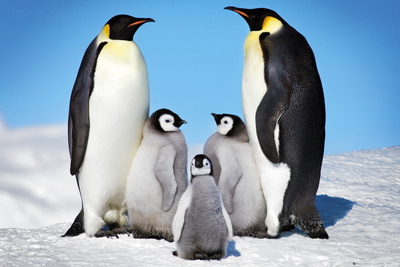
\includegraphics[scale=.50]{figures/Penguins.jpg}
% \caption{Another TAMU figure.}
% \label{fig:tamu-fig6}
% \end{figure}

% \section{Appendix Section}

% \section{Second Appendix Section}			% Include the appendix2.tex file
\end{appendices}

\end{document}
